% 16 Component Dirac Fermion Condensate Singlet Superfluid on 4+4 Deflating Spacetime
% REVTeX 4.2, Physical Review D, two-column.
%
% This file is self-contained: every definition, equation and symbol that it uses is in it, and
% the reference list is embedded at the end, so that no BibTeX run is needed.  Build (three runs
% settle all cross references), from the directory Revision_Deflation_CJT_and_Kohn-Sham_definition_C/manuscript/
% of the repository (the figures are read from ../figures/):
%
%     pdflatex "16 Component Dirac Fermion Condensate Singlet Superfluid on 4+4 Deflating Spacetime.tex"
%
% DO NOT EDIT THIS FILE BY HAND.  It is assembled by code/scripts/build_manuscripts.py from the
% source files in docs_src/manuscript/, and every computed number is inserted by that script from
% the data files in data/ (Appendix "Programs, checks and provenance" of this file says how).
\documentclass[aps,prd,twocolumn,floatfix,nofootinbib,longbibliography]{revtex4-2}

\usepackage{amsmath,amssymb,bm}
\usepackage{graphicx}
\usepackage{dcolumn}
\usepackage{array}
\usepackage{booktabs}
\usepackage{xcolor}
\usepackage[colorlinks=true,linkcolor=blue!50!black,citecolor=blue!50!black,urlcolor=blue!50!black]{hyperref}
\graphicspath{{../figures/}}
\raggedbottom
\hypersetup{pdftitle={16 Component Dirac Fermion Condensate Singlet Superfluid on 4+4 Deflating Spacetime},
  pdfauthor={Patrick Lee Nash}}
% the same source always gives the same PDF file (no time stamp, no random identifier)
\ifdefined\pdfinfoomitdate\pdfinfoomitdate=1 \pdftrailerid{}\pdfsuppressptexinfo=-1 \fi
\setcounter{topnumber}{3}
\setcounter{bottomnumber}{2}
\setcounter{totalnumber}{5}
\setcounter{dbltopnumber}{3}
\renewcommand{\topfraction}{0.9}
\renewcommand{\bottomfraction}{0.6}
\renewcommand{\textfraction}{0.08}
\renewcommand{\floatpagefraction}{0.9}
\renewcommand{\dbltopfraction}{0.9}
\renewcommand{\dblfloatpagefraction}{0.9}

% ---------------------------------------------------------------- macros
% the tag that marks every object of the spacetime of this paper
\newcommand{\tg}{1644d}
% the three rates of deflation (the names of the hypotheses: upright, never with a subscript), and their combinations
\newcommand{\gff}{\mathrm{g55}}
\newcommand{\gss}{\mathrm{g66}}
\newcommand{\gvv}{\mathrm{g77}}
\newcommand{\gsum}{\mathrm{gsum}}
\newcommand{\gsq}{\mathrm{gsq}}
\newcommand{\gprod}{\mathrm{gprod}}
\newcommand{\rt}{\mathrm{rate}_t}
\newcommand{\cff}{\mathrm{const5}}
\newcommand{\css}{\mathrm{const6}}
\newcommand{\cvv}{\mathrm{const7}}
\newcommand{\ct}{\mathrm{const}_t}
% deflating volume, clock, weighted field
\newcommand{\Vd}{V_d}
\newcommand{\td}{\tau_d}
\newcommand{\tpair}{\tau_{\mathrm{pair}}}
\newcommand{\hpsi}{\hat\psi}
\newcommand{\Eperp}{E_\perp}
\newcommand{\kd}{k_d}
\newcommand{\ud}{u_d}
\newcommand{\ncr}{n_{\mathrm{cr}}}
\newcommand{\Tdefl}{T_{\mathrm{defl}}}
\newcommand{\Swkb}{S_{\mathrm{WKB}}}
\newcommand{\Xid}{\Xi_d}
\newcommand{\Deq}{\Delta_{\mathrm{eq}}}
\newcommand{\Esh}{E_{\mathrm{sh}}}
\newcommand{\nex}{n_{\mathrm{ex}}}
\newcommand{\nEW}{n_{\mathrm{EW}}}
\newcommand{\vEW}{v_{\mathrm{EW}}}
\newcommand{\GN}{G_N}
\newcommand{\aGB}{\alpha_{\mathrm{GB}}}
\newcommand{\Lam}{\Lambda_8}
\newcommand{\cG}{\mathcal{G}}
\newcommand{\cH}{\mathcal{H}}
\newcommand{\cX}{\mathcal{X}}
% perturbations of ordinary space (Sec. XI): conformal time, conformal Hubble rate, metric functions of the synchronous
% gauge, sums over matter and radiation, gaps
\newcommand{\tcf}{\tau_{\mathrm{cf}}}
\newcommand{\Hcf}{H_{\mathrm{cf}}}
\newcommand{\He}{H_e}
\newcommand{\hsy}{h_{\mathrm{sy}}}
\newcommand{\etasy}{\eta_{\mathrm{sy}}}
\newcommand{\alsy}{\alpha_{\mathrm{sy}}}
\newcommand{\cD}{\mathcal{D}}
\newcommand{\cT}{\mathcal{T}}
\newcommand{\cP}{\mathcal{P}}
\newcommand{\cA}{\mathcal{A}}
\newcommand{\cE}{\mathcal{E}}
\newcommand{\cB}{\mathcal{B}}
\newcommand{\cZ}{\mathcal{Z}}
\newcommand{\cYM}{\mathcal{Y}_M}
\newcommand{\cYT}{\mathcal{Y}_T}
\newcommand{\cYS}{\mathcal{Y}_S}
\newcommand{\YHe}{Y_{\mathrm{He}}}
% the Vorton-Scalar and its parameters
\newcommand{\PhiVS}{\Phi_{\mathrm{VS}}}
\newcommand{\vVS}{v_{\mathrm{VS}}}
\newcommand{\gVS}{g_{\mathrm{VS}}}
\newcommand{\aVS}{\alpha_{\mathrm{VS}}}
\newcommand{\DVS}{D_{\mathrm{VS}}}
\newcommand{\lamVS}{\lambda_{\mathrm{VS}}}
\newcommand{\yVS}{y_{\mathrm{VS}}}
\newcommand{\GVS}{G_{\mathrm{VS}}}
\newcommand{\UVS}{U(1)_{\mathrm{VS}}}
% general
\newcommand{\kF}{k_F}
\newcommand{\EF}{E_F}
\newcommand{\Cm}{C^{-}}
\newcommand{\hh}{\mathsf{h}}
\newcommand{\MM}{\mathsf{M}}
\newcommand{\kmsMpc}{\mathrm{km\,s^{-1}\,Mpc^{-1}}}
% the metric of the deflating spacetime in the sign convention of the hypothesis (space-like
% components positive, time-like components negative): g^{(4+4)} or g^{(7+1)}; its inverse; the flat metric
\newcommand{\gm}{g^{(4+4)}}
\newcommand{\gmup}[1]{g_{(4+4)}^{#1}}
\newcommand{\etam}{\eta^{(4+4)}}
\newcommand{\etamup}[1]{\eta_{(4+4)}^{#1}}
% mass term and self-interaction
\newcommand{\Lself}{\mathcal{L}_{\mathrm{self}}}
\newcommand{\sgnK}{\mathrm{sgn}_K}
\newcommand{\geff}[1]{g_{#1}^{\mathrm{eff}}}
\newcommand{\sfF}{\mathsf{F}}
\newcommand{\sfn}{\mathsf{n}}
\newcommand{\Gpair}{G_{\mathrm{pair}}}
% the two halves of the 4+4 field and the two forms of its self-interaction
\newcommand{\Wg}{W_{1644}}
\newcommand{\LselfC}{\mathcal{L}_{\mathrm{self}}^{\mathrm{C}}}
\newcommand{\LselfQ}{\mathcal{L}_{\mathrm{self}}^{\mathrm{Q}}}
\newcommand{\ThQ}{\Theta_Q}
\newcommand{\sgnQ}{\mathrm{sgn}_K^{Q}}
\newcommand{\GStot}{G_S^{\mathrm{tot}}}
\newcommand{\GVtot}{G_V^{\mathrm{tot}}}
\newcommand{\GSdif}{G_S^{\mathrm{dif}}}
\newcommand{\GVdif}{G_V^{\mathrm{dif}}}
\newcommand{\GSsame}{G_S^{\mathrm{same}}}
\newcommand{\GVsame}{G_V^{\mathrm{same}}}
\newcommand{\GSopp}{G_S^{\mathrm{opp}}}
\newcommand{\GVopp}{G_V^{\mathrm{opp}}}
\newcommand{\mstpm}{m^{*}_{\pm}}
\newcommand{\sct}{s_{\mathrm{ct}}}
\newcommand{\kmax}{k_{\max}}
\newcommand{\Uuv}{U_{\mathrm{uv}}}
% Kohn-Sham and CJT calculations
\newcommand{\mst}{m^{*}}
\newcommand{\mstq}{m^{*2}}
\newcommand{\nS}{n_S}
\newcommand{\GS}{G_S}
\newcommand{\GV}{G_V}
\newcommand{\pint}{p_{\mathrm{int}}}
\newcommand{\mct}{m_{\mathrm{ct}}}
\newcommand{\mth}{m_{\vartheta}}
% gravity with two scale factors
\newcommand{\ma}{\mathsf{a}}
\newcommand{\mb}{\mathsf{b}}

\begin{document}

\title{16 Component Dirac Fermion Condensate Singlet Superfluid on 4+4 Deflating Spacetime}

\author{Patrick Lee Nash, Ph.D.}
\affiliation{Independent researcher}

\date{November 13, 2026}

\begin{abstract}
A 16-component Dirac field with a mass term and a quartic self-interaction is studied on a spacetime
with four space-like and four time-like dimensions in which three of the time-like coordinates
deflate exponentially as the ordinary time advances. The Dirac equation is solved exactly: every
admissible mode that depends on a deflating time is extinguished, and fields that do not depend on
the deflating times obey the flat equations with couplings that grow with the deflation. Of the
nine couplings of the self-interaction only four are independent. In the sector that can be
quantized the self-interaction has two forms, which differ by a sign between the two halves of the
field; the covariant form is the definition, and the other is given beside it. Matter and vacuum
are analyzed with the Kohn-Sham method and with the effective action of Cornwall, Jackiw and
Tomboulis, which agree. In the covariant form a gas polarizes and becomes self-bound matter with one
half of the field filled, a massless field acquires masses of opposite sign in the two halves, and
the self-interaction distinguishes the fermion pair along the hidden axis from the pairs along the
additional times, each at a definite moment of the deflation. With equal rates the spacetime solves
Einstein-Gauss-Bonnet gravity without matter; the solution is unstable, and matter accelerates the
deflation. Bounds on the rate from cosmology and from atomic clocks are given.
\end{abstract}

\maketitle

\section{Introduction}
\label{sec:intro}

\subsection{The question}

This paper studies a single fermion field with sixteen complex components on a spacetime of eight
dimensions. Two such spacetimes are of interest. One has four space-like and four time-like
dimensions, and is written $4{+}4$; the other has seven space-like dimensions and one time-like
dimension, and is written $7{+}1$. On both, the eight Dirac matrices can be chosen real
\cite{Nash1984,Nash1990,Nash2010}, and the field
supports a superfluid of fermion pairs of spin zero whose order parameter points along one of the
four coordinates that are not the coordinates of ordinary spacetime. This paper treats the $4{+}4$
spacetime. Spacetimes with more than one time have been studied for their own sake
\cite{Bars2001}; what a second time does to the evolution of a field is taken up in
Sec.~\ref{sec:modes}.

The eight coordinates are written $x0,x1,\dots,x7$. Throughout, $x1,x2,x3$ are the coordinates of
ordinary space and $x4$ is the ordinary time. The coordinate $x0$ is an additional space-like
coordinate, called the hidden coordinate. The remaining three, $x5,x6,x7$, are
three additional \emph{time-like} coordinates.

On a flat spacetime nothing explains why the fields of ordinary physics do not depend on $x5$, $x6$
and $x7$. On the $4{+}4$ spacetime this is more than a gap in the explanation. A field that
depends on an additional time does not evolve unitarily in the ordinary time, and on flat spacetime
one has to \emph{impose} that the fields do not depend on the additional times. The present paper examines a definite proposal for what happens to
these three coordinates, and it does so for a field with a mass and with a self-interaction.

\subsection{The hypothesis of deflation}

The hypothesis is that \emph{the coordinates $x5$, $x6$ and $x7$ deflate exponentially}: as the
ordinary time $x4$ advances, the proper extent of every interval along each of these coordinates
shrinks as an exponential of $x4$. Flat spacetime is replaced by a curved spacetime with a diagonal
metric, in which the three components of the metric along the deflating coordinates are
\begin{equation}
\begin{aligned}
\gm_{55}&=-\cff^{2}\,e^{-2\,\gff\,x4},\\
\gm_{66}&=-\css^{2}\,e^{-2\,\gss\,x4},\\
\gm_{77}&=-\cvv^{2}\,e^{-2\,\gvv\,x4}.
\end{aligned}
\label{eq:hyp}
\end{equation}
Here $\gff$, $\gss$ and $\gvv$ are three positive constants, the \emph{rates} of deflation; $\cff$,
$\css$ and $\cvv$ are three positive constants that set the scale at $x4=0$ and may differ from one
another. The names of the rates are written upright and without a subscript, to distinguish them
from the components $\gm_{55}$, $\gm_{66}$, $\gm_{77}$ of the metric, which carry subscripts and the
superscript $(4+4)$. The other five components of the metric keep their flat values,
$+1$ for $x0,\dots,x3$ and $-1$ for the time $x4$. The sign convention is that space-like components
of the metric are positive and time-like components negative: the minus signs in
Eq.~(\ref{eq:hyp}) say that $x5,x6,x7$ are time-like.

\subsection{Mass term, self-interaction, and the two methods}

The Lagrangian of the fermion field has three parts (Sec.~\ref{sec:dirac}): the kinetic term; a
\emph{mass term}, bilinear in the field; and a \emph{self-interaction}, quartic in the field. The
self-interaction is the most general one without derivatives: nine invariants, one for each number
$r=0,\dots,8$ of Dirac matrices in the bilinears from which it is built, with nine couplings $g_r$.
The field equation is a nonlinear Dirac equation. The paper answers the following questions about
it. How many of the nine couplings are independent? What do the mass term and the self-interaction
do to matter made of these fermions, on flat spacetime and while three coordinates deflate? What do
they do to the pairing of the fermions, which in this model is mediated by a second field, the
Vorton-Scalar? And what does such matter do to the spacetime itself, if it is the source of gravity?

Two methods are used throughout, and each checks the other.
\begin{itemize}
\item The \emph{Kohn-Sham method}, known from density-functional theory: the interacting fermions
are replaced by independent fermions that move in fields which are determined self-consistently by
their own densities. For uniform matter the fields are a shift of the mass and a shift of the
energy.
\item The \emph{effective potential for composite operators} of Cornwall, Jackiw and Tomboulis
(CJT): a function of the full propagator of the fermions whose stationary points are the possible
states of matter and whose value there is minus the pressure.
\end{itemize}
The two methods are equivalent at the level of approximation used here, and the paper verifies this
numerically (Sec.~\ref{sec:cjtcontact}).

The paper also examines three hypotheses about the superfluid.
\begin{itemize}
\item[H1.] The fermion field forms a superfluid state of spin 0 in which the fermions are paired by
the exchange of a new scalar boson, the \emph{Vorton-Scalar}, through a neutral current of the kind
known from the weak interaction.
\item[H2.] This superfluid state is the Higgs field.
\item[H3.] This superfluid state explains the observations of dark matter, or the Hubble tension, or
both.
\end{itemize}
The purpose is to carry out every calculation that these hypotheses call for under the hypothesis of
deflation, with the mass term and the self-interaction, and to report what follows for H1, H2 and
H3, favorable or not.

\subsection{Summary of results}

\emph{Geometry} (Sec.~\ref{sec:geometry}). The deflating spacetime is homogeneous and has 14
symmetries, or 15 or 20 if two or three of the rates are equal, instead of the 36 of flat spacetime.
It is not a solution of Einstein's equations without matter. With three equal rates it \emph{is} an
exact solution of the equations of Einstein-Gauss-Bonnet gravity without matter, for one definite
relation between the rate and the two constants of that theory.

\emph{The Dirac field} (Secs.~\ref{sec:dirac}, \ref{sec:modes}). A field that does not depend on
$x5,x6,x7$ obeys, after multiplication by the square root of the volume factor of the deflating
coordinates, exactly the flat equation with the mass unchanged and with every coupling of the
self-interaction growing as the exponential of the time. A field that does depend on the deflating
coordinates is affected directly.
The linear equation is solved exactly. Of its sixteen solutions eight grow as the exponential of an
exponential of the time and are not admissible. The other eight are standing waves, which are
extinguished as the exponential of an exponential. \emph{The deflation removes the dependence of the
field on the additional times}, and with it the sector in which the $4{+}4$ theory is not unitary.

\emph{The self-interaction} (Sec.~\ref{sec:selfint}). For anticommuting fields the nine invariants
obey five linear relations: only four couplings are independent, a scalar, a vector, an axial-vector
and a pseudoscalar one. Uniform matter feels two combinations of them, pairs of particles at rest
feel a third. On the $4{+}4$ spacetime the self-interaction has two forms in the sector that can
be quantized, which agree for particles in the same half of the field and differ in sign for
particles in different halves. The covariant form is the definition of the model in this paper;
the other is recorded beside it, and the two are discussed in Sec.~\ref{sec:formsdisc}.

\emph{Matter} (Secs.~\ref{sec:ks}, \ref{sec:cjtcontact}). The Kohn-Sham method and the CJT effective
potential give the same states. In the sector of fields
that do not depend on the deflating coordinates a scalar attraction grows with the deflation and
turns a gas into self-bound matter at a definite moment. With the filled states of negative energy
taken into account, the same growth gives a massless field a mass at a critical coupling. In
the covariant form matter polarizes: the self-bound state fills one half of the field and forms at
two to three times the strength that the alternative form needs, and the mass that a massless field
acquires has opposite signs in the two halves. A bare
mass together with the Vorton-Scalar gives the phase mode of that field a mass.

\emph{The superfluid} (Secs.~\ref{sec:clock} to \ref{sec:order}). For fields that do not depend on
the extra coordinates the pairing calculation of flat spacetime holds at each moment with the
couplings of that moment. The masses do not change. Every threshold is passed at a definite time. The
gap of the paired state grows much faster than the coupling; in the pairs along the additional
times a scalar contact attraction raises it and a vector contact repulsion lowers it, and in the
pair along the hidden axis the covariant form reverses both. The gap equation has a solution that does not depend on the
upper limit of its momentum integral only below an ultraviolet criterion. Two fermions become bound at a scattering resonance. The
paired state can follow the deflation only once its gap exceeds a few times the rate divided by the
pairing strength; before that it lags behind and breaks pairs. Matter of a given density loses its
fermion mass at a definite time. A vortex line carries four fermion zero modes.

\emph{Gravity} (Sec.~\ref{sec:gravity}). With Kohn-Sham matter as the source of the Einstein-Lovelock
equations the deflating spacetime is not stationary: the three coordinates deflate faster than
exponentially and the four flat coordinates expand. Even without matter the exactly exponential
deflation is an unstable solution of the gravity in which it is a solution.

\emph{Cosmology} (Sec.~\ref{sec:cosmo}). If gravity is the Einstein theory in eight dimensions,
Newton's constant grows at the total rate of deflation; lunar laser ranging then bounds that rate to
$3\times10^{-3}$ of the Hubble rate, and the Hubble constant inferred from the microwave background
falls. The deflation does not relieve the Hubble tension. Whatever keeps the rates constant must
carry a tension and must take part in the perturbations of ordinary space; the spectra of the
microwave background at all but the largest angular scales do not depend on how it does so, and
the growth of structure does.

\emph{The Higgs hypothesis} (Sec.~\ref{sec:higgs}). The symmetry under which the pair condensate
has the pattern of the Higgs vacuum is a hidden symmetry on the $4{+}4$ spacetime, flat or deflating. A contact self-interaction of the covariant form breaks it explicitly, down to the
rotations of the additional times. If the
condensate were the Higgs field, the electroweak scale would follow the growing coupling, and atomic
clocks would limit the rate of deflation to about $10^{-6}$ of the Hubble rate. The hypothesis H2 and
a deflation of any consequence today exclude each other.

\subsection{Method, and the limits of what is claimed}

Every statement of this paper about geometry, matrices and operators is an identity that a program
has verified in exact rational arithmetic, and that an independent program has verified again by
computer algebra or with Grassmann-valued fields. Every numerical statement is the output of a
program, with a stated accuracy, and the central ones were computed twice by independent programs.
The programs and their output are public \cite{DeflationRepo}; Appendix~\ref{app:checks} says how each
number of this paper is reproduced. The program performs 310 checks and the independent
verification 88, all of which pass. The metric of Eq.~(\ref{eq:hyp}) is a
hypothesis. The paper derives its consequences; it does not claim that the hypothesis is true.
Section~\ref{sec:status} lists what has been established and what has not.

Units are natural, $\hbar=c=k_B=1$. Symbols that carry the tag $\tg$ refer to the deflating
$4{+}4$ spacetime. A general coordinate among the three deflating ones is written $xt$ with
$t\in\{5,6,7\}$ and its rate $\rt$; a general coordinate among $x0,x1,x2,x3$ is written $xj$ with
$j\in\{0,1,2,3\}$. The letter $a$ is kept for the four extra axes, $a\in\{0,5,6,7\}$
(Sec.~\ref{sec:gap}). Every symbol is defined where it first appears, and Appendix~\ref{app:symbols}
lists all of them.

\section{The deflating spacetime}
\label{sec:geometry}

This section derives the geometry that the hypothesis implies: the curvature, the field equations
that the metric does and does not solve, its symmetries, and the motion of a classical particle.
Every formula of this section was obtained twice by exact computer algebra, by the program of this
paper and by an independent script (Appendix~\ref{app:checks}); the steps are short enough to be
repeated by hand, and the text says how.

\subsection{Metric, frame and volume}

Throughout, the metric is written in the sign convention of the hypothesis (\ref{eq:hyp}):
\emph{space-like components are positive and time-like components are negative}. The flat metric is
\begin{equation}
\etam=\mathrm{diag}(+1,+1,+1,+1,-1,-1,-1,-1),
\label{eq:etam}
\end{equation}
with the coordinates in the order $x0,\dots,x7$: four space-like coordinates $x0,\dots,x3$ and
four time-like ones, $x4,\dots,x7$. Define three \emph{scale factors}, one for each deflating coordinate,
\begin{equation}
b_t(x4)=\ct\,e^{-\rt\,x4},\qquad t=5,6,7,
\label{eq:scale}
\end{equation}
with $\mathrm{rate}_5=\gff$, $\mathrm{rate}_6=\gss$, $\mathrm{rate}_7=\gvv$. The metric of the
deflating spacetime is
\begin{equation}
\gm_{\mu\nu}=\mathrm{diag}\big(+1,+1,+1,+1,-1,\,-b_5^2,\,-b_6^2,\,-b_7^2\big),
\label{eq:metric}
\end{equation}
whose last three components are those of Eq.~(\ref{eq:hyp}). The superscript $(4+4)$
marks the metric of this spacetime in this sign convention; a component of the metric always
carries it, so that $\gm_{55}$ cannot be taken for the rate $\gff$. Greek indices label the
coordinates. A
coordinate interval $dxt$ has the proper extent $b_t\,|dxt|$, which shrinks by the factor $e$ in the
time $1/\rt$. Because $x5,x6,x7$ are time-like, what shrinks is a duration measured along an
additional time.

Capital indices $A,B$ label an orthonormal frame, eight vector fields $e_A=e_A{}^{\mu}\partial_\mu$
with $\gm_{\mu\nu}e_A{}^{\mu}e_B{}^{\nu}=\etam_{AB}$. We take the frame along the coordinates,
$e_A{}^{\mu}=\mathrm{diag}(1,1,1,1,1,b_5^{-1},b_6^{-1},b_7^{-1})$. The volume element is $\Vd\,d^8x$
with
\begin{equation}
\Vd(x4)=b_5b_6b_7\propto e^{-\gsum\,x4},\quad\gsum=\gff+\gss+\gvv .
\label{eq:Vd}
\end{equation}
$\Vd$ is the proper volume of a unit coordinate cell of the deflating coordinates, and the
\emph{total rate} $\gsum$ is the rate at which it shrinks. Most results below depend on the three
rates only through $\gsum$.

\subsection{Curvature}
\label{sec:curvature}

The only components of the metric that depend on a coordinate are the three $\gm_{tt}$, and they
depend on $x4$ alone. The Christoffel symbols
$\Gamma^{\rho}{}_{\mu\nu}=\tfrac12g^{\rho\sigma}(\partial_\mu g_{\sigma\nu}+\partial_\nu g_{\sigma\mu}-\partial_\sigma g_{\mu\nu})$
that do not vanish are therefore
\begin{equation}
\Gamma^{t}{}_{4t}=-\rt,\qquad\Gamma^{4}{}_{tt}=+\rt\,b_t^{2},
\end{equation}
without summation over $t$. The Riemann tensor has, in the orthonormal frame, the components
\begin{equation}
R^{t}{}_{4t4}=-\rt^{2},\quad R^{t}{}_{sts}=-\rt\,\mathrm{rate}_s\ \ (t\ne s),
\label{eq:riemann}
\end{equation}
and those related to them by symmetry. No component carries an index of $x0,\dots,x3$: these four
coordinates span a flat space, and the curvature lives in the four coordinates $x4,\dots,x7$. With
$\gsq=\gff^2+\gss^2+\gvv^2$ and $\gprod=\gff\gss+\gff\gvv+\gss\gvv$, the curvature scalar is the
constant $R=\gsq+\gsum^{2}$, and the Einstein tensor
$\cG^{\mu}{}_{\nu}=R^{\mu}{}_{\nu}-\tfrac12R\,\delta^{\mu}_{\nu}$ is diagonal with
\begin{equation}
\begin{aligned}
\cG^{4}{}_{4}&=-\gprod,\qquad\cG^{j}{}_{j}=-\tfrac12(\gsq+\gsum^{2}),\\
\cG^{t}{}_{t}&=\rt\,\gsum-\tfrac12(\gsq+\gsum^{2}),
\end{aligned}
\label{eq:einstein}
\end{equation}
with $j=0,1,2,3$. In the sign convention used here these mixed components are the same on the $4{+}4$
and on the $7{+}1$ spacetime. (They follow from the sectional curvatures of Appendix~\ref{app:curvature}:
$\cG^{A}{}_{A}$ is minus the sum of the sectional curvatures of the planes that do not contain the
direction $A$.)
The Einstein tensor does not vanish, and it is not a multiple of the unit matrix unless all rates
vanish. \emph{The deflating spacetime is not a solution of Einstein's equations without matter, with
or without a cosmological constant.}

\subsection{A solution of Einstein-Gauss-Bonnet gravity}
\label{sec:egb}

In more than four dimensions the general field equations of second order for the metric are those of
Lovelock \cite{Lovelock1971}. Their first term beyond Einstein's is the Lanczos tensor
$\cH^{\mu}{}_{\nu}$ of the Gauss-Bonnet term \cite{BoulwareDeser1985}, and the equations without
matter read
\begin{equation}
\cG^{\mu}{}_{\nu}+\Lam\,\delta^{\mu}_{\nu}+\aGB\,\cH^{\mu}{}_{\nu}=0,
\label{eq:egb}
\end{equation}
with a cosmological constant $\Lam$ and a coupling $\aGB$. For the metric
(\ref{eq:metric}) we find
\begin{equation}
\begin{aligned}
\cH^{j}{}_{j}&=-4\,\gff\,\gss\,\gvv\,\gsum\quad(j=0,1,2,3),\\
\cH^{4}{}_{4}&=\cH^{t}{}_{t}=0,
\end{aligned}
\label{eq:lanczos}
\end{equation}
and the Lovelock tensor of the third order, the last that can differ from zero in eight dimensions,
vanishes identically. The components of Eq.~(\ref{eq:egb}) along $x4,\dots,x7$ therefore contain no
Gauss-Bonnet term and require the four corresponding components of the Einstein tensor to be equal,
which holds if and only if the three rates are equal. The components along $x0,\dots,x3$ then fix the
coupling. The result:
\begin{equation}
\gff=\gss=\gvv:\qquad\Lam=3\,\gff^{2},\qquad\aGB=-\frac{1}{4\,\gff^{2}} .
\label{eq:egbsol}
\end{equation}
\emph{With three equal rates the deflating spacetime is an exact solution of Einstein-Gauss-Bonnet
gravity without matter}, in a theory whose two constants satisfy $4\aGB\Lam=-3$; the rate is then
$\gff=\sqrt{\Lam/3}$. With unequal rates it is not a solution for any $\Lam$ and $\aGB$. Solutions of
this theory in which every scale factor is an exponential of the time have been classified in five
and six dimensions \cite{ChirkovPavluchenkoToporensky2014}; the present one, with four static and
three contracting directions in eight dimensions, is of that kind. In the notation of the
Einstein-Lovelock equations of Sec.~\ref{sec:gravity}, Eq.~(\ref{eq:egbsol}) reads
$\bar\Lambda=3\,\gff^{2}$, $\alpha_2=1/(4\,\gff^{2})$. Section~\ref{sec:gravity} examines the
stability of this solution, with and without matter: it is unstable.

\subsection{Symmetries}

A Killing vector is a vector field along which the metric does not change. Flat spacetime in eight
dimensions has 36. The deflating spacetime has, for any rates, 14: the seven translations along all
coordinates but $x4$; the six rotations of $x0,x1,x2,x3$; and the scaling
\begin{equation}
\cX_{\mathrm{scale}}=\partial_4+\gff\,x5\,\partial_5+\gss\,x6\,\partial_6+\gvv\,x7\,\partial_7,
\label{eq:scaling}
\end{equation}
which shifts the time and stretches the deflating coordinates so as to undo the shrinking. Two equal
rates add the rotation of the two coordinates concerned. Three equal rates add the three rotations of
$x5,x6,x7$ and three further vectors, 20 in all; the four coordinates $x4,\dots,x7$ then form a space
of constant curvature of radius $1/\gff$:
minus a four-dimensional hyperbolic space. These lists are complete. (A Killing vector that vanishes at a point is a
Lorentz transformation of the tangent space that leaves the Riemann tensor (\ref{eq:riemann})
unchanged; the dimension of the space of such transformations is 6, 7 or 12, which bounds the number
of Killing vectors by 14, 15 or 20.)

Three consequences are used below. The spacetime is homogeneous: no place and no moment is
distinguished. The constants $\ct$ are not observable by themselves, since a rescaling of $xt$
changes them; the deflation is observable only through an object that fixes a coordinate scale along
$xt$, such as a wave of given coordinate wavelength. And there is no conserved energy, because a
translation in time alone is not a symmetry.

Of the 28 rotations and boosts of flat spacetime, only the six rotations of $x0,\dots,x3$ survive for
general rates (Fig.~\ref{fig:isometries}, Table~\ref{tab:xisometries}). Nothing that involves the time survives, in particular
not the boosts of ordinary special relativity: the deflation defines a preferred state of rest, as
the expansion of the universe does.

\begin{figure*}
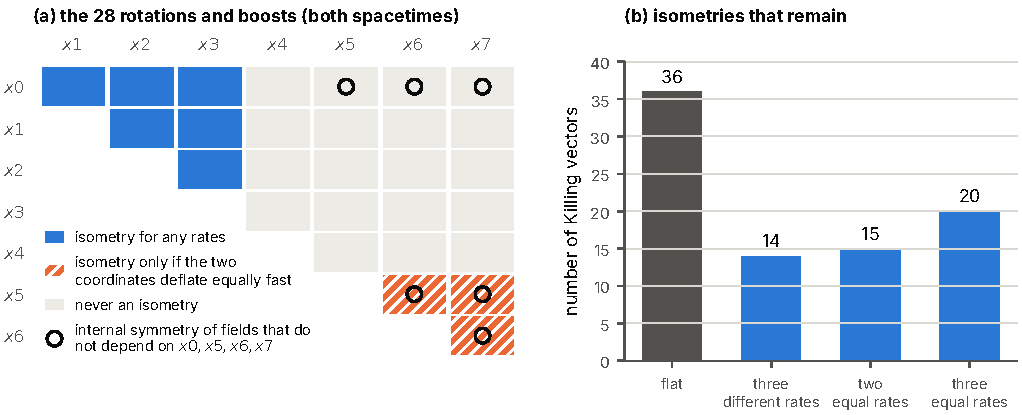
\includegraphics[width=0.86\textwidth]{fig_isometries}
\caption{\label{fig:isometries}Symmetries of the deflating spacetime. (a) The 28 rotations and boosts
of flat spacetime, one square for each pair of coordinates: those that remain symmetries for any
rates, those that remain symmetries only if the two coordinates deflate equally fast, and those that
are never symmetries. Circles mark the six pairs whose rotations act as internal symmetries on fields
that do not depend on $x0,x5,x6,x7$ (Sec.~\ref{sec:higgs}). (b) The number of Killing vectors.}
\end{figure*}

\subsection{Geodesics}
\label{sec:geodesics}

The translations give seven conserved momenta $P_\mu$ ($\mu\ne4$) of a classical particle. Let
$\Eperp=(m^{2}+\sum_jP_j^{2})^{1/2}$, with the sum over $j=0,1,2,3$, be the energy that a particle of
mass $m$ would have without momentum along the deflating coordinates. The conservation of the norm of the momentum gives the
velocity along the time, with an affine parameter $\varsigma$ along the path:
\begin{equation}
\Big(\frac{dx4}{d\varsigma}\Big)^{2}=\Eperp^{2}-\sum_{t}\frac{P_t^{2}}{b_t(x4)^{2}} .
\label{eq:geodesic}
\end{equation}
The last term grows as $e^{2\,\rt\,x4}$: the momentum $P_t$ belongs to a fixed coordinate wavelength,
and the proper wavelength shrinks.
With the minus sign the right-hand side vanishes at a \emph{turning value} of the time; for momentum
along $x5$ alone,
\begin{equation}
x4_{\mathrm{turn}}=\frac{1}{\gff}\ln\frac{\Eperp\,\cff}{|P_5|} .
\label{eq:turn}
\end{equation}
The path reaches this value and returns to smaller $x4$ [Fig.~\ref{fig:geodesics}(b)]. A classical
particle with momentum along a deflating time cannot pass the turning value of the ordinary time. Section~\ref{sec:modes} shows the
quantum form of this result. (On the $7{+}1$ spacetime the sign in Eq.~(\ref{eq:geodesic}) is the
opposite, and the energy of such a particle grows without bound.)

\begin{figure*}
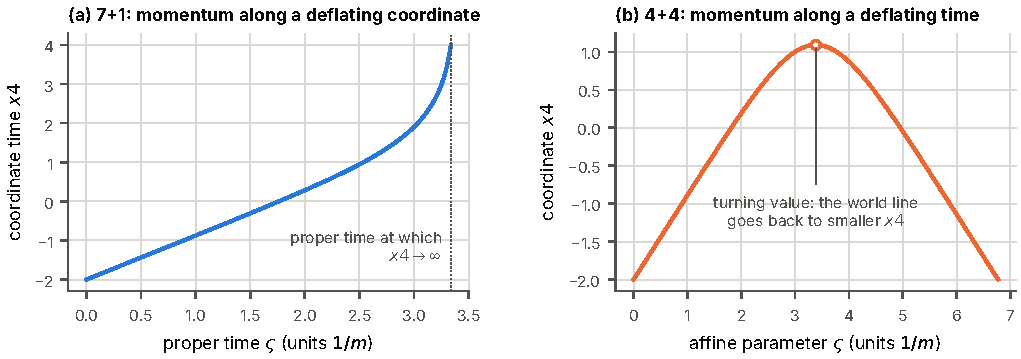
\includegraphics[width=0.8\textwidth]{fig_geodesics}
\caption{\label{fig:geodesics}A classical particle of the mass $m=1$ with the momenta $P_1=0.5$ along
$x1$ and $P_5=0.3$ along the deflating coordinate $x5$, for $\gff=1$ and $\cff=0.8$, started at
$x4=-2$. (a) On the $7{+}1$ spacetime the time $x4$ grows without bound within the finite proper time
3.386. (b) On the $4{+}4$ spacetime the path reaches the turning value $x4=1.0924$ and returns to
smaller $x4$.}
\end{figure*}

\section{The Dirac field with mass term and self-interaction}
\label{sec:dirac}

\subsection{Matrices and spin connection}

At each point of a curved spacetime the tangent space is flat. The Dirac matrices of the orthonormal
frame are therefore eight constant matrices $\gamma^{A}$, $A=0,\dots,7$. They are real $16\times16$
matrices with entries $0$ and $\pm1$, printed in full in Appendix~\ref{app:matrices}.
The four matrices of the space-like coordinates are symmetric and square to $+1$, the four matrices
of the time-like coordinates are antisymmetric and square to $-1$, and different matrices
anticommute:
\begin{equation}
\gamma^{A}\gamma^{B}+\gamma^{B}\gamma^{A}=2\,\etamup{AB} .
\label{eq:clifford}
\end{equation}
All of these properties were verified by exact integer arithmetic for this work. The matrices with a
coordinate index are $\gamma^{\mu}=e_A{}^{\mu}\gamma^{A}$: five of them are the constant matrices,
and the three along the deflating coordinates are the constant matrices divided by the scale
factors, $\gamma^{A=t}/b_t$. They satisfy
$\gamma^{\mu}\gamma^{\nu}+\gamma^{\nu}\gamma^{\mu}=2\,\gmup{\mu\nu}$ with the inverse
metric $\gmup{\mu\nu}$.

A spinor is defined relative to a frame, and its derivative must account for the turning of the frame
from point to point \cite{BrillWheeler1957}. The covariant derivative of a spinor is
$\nabla_\mu\psi=(\partial_\mu+\Omega_\mu)\psi$ with the spin connection
\begin{equation}
\begin{aligned}
\Omega_\mu&=\tfrac14\,\omega_{\mu AB}\,\gamma^{A}\gamma^{B},\\
\omega_{\mu AB}&=\etam_{AC}\,e^{C}{}_{\nu}\big(\partial_\mu e_B{}^{\nu}+\Gamma^{\nu}{}_{\mu\lambda}e_B{}^{\lambda}\big),
\end{aligned}
\label{eq:spindef}
\end{equation}
whose coefficients $\omega_{\mu AB}=-\omega_{\mu BA}$ follow from the metric ($e^{C}{}_{\nu}$ is
the inverse of the frame). For the
metric (\ref{eq:metric}) the only coefficients that do not vanish are
$\omega_{t\,t4}=-\omega_{t\,4t}=\rt\,b_t$, so that
\begin{equation}
\begin{aligned}
\Omega_t&=\tfrac12\,\rt\,b_t\,\gamma^{t}\gamma^{4}\quad(t=5,6,7),\\
\Omega_0&=\dots=\Omega_4=0,
\end{aligned}
\label{eq:spinconn}
\end{equation}
with the constant matrices of the frame on the right. Each $\Omega_t$ generates the Lorentz
transformation in the plane of $xt$ and $x4$. The spin connection is correct if and only if the
Dirac matrices are covariantly constant,
$\partial_\mu\gamma^{\nu}+\Gamma^{\nu}{}_{\mu\lambda}\gamma^{\lambda}+[\Omega_\mu,\gamma^{\nu}]=0$,
which holds for all 64 pairs of indices. Its curvature is the Riemann tensor,
$[\nabla_\mu,\nabla_\nu]\psi=\tfrac14R_{AB\mu\nu}\gamma^{A}\gamma^{B}\psi$, a third route to
Eq.~(\ref{eq:riemann}). One combination enters the Dirac equation:
\begin{equation}
\gamma^{\mu}\Omega_\mu=-\tfrac12\,\gsum\,\gamma^{4} .
\label{eq:gammaomega}
\end{equation}
The scale factors cancel, and only the total rate remains.

\subsection{The Lagrangian: kinetic term, mass term, self-interaction}
\label{sec:lagrangian}

The field of this paper, $\psi_{\tg}(x)$, is a column of sixteen complex-valued Grassmann operators.
Its Lagrangian has three parts,
\begin{equation}
\mathcal L_{\tg}=\Vd\,\big[\mathcal L_{\mathrm{kin}}+\mathcal L_{\mathrm{mass}}+\Lself\big],
\label{eq:Ltot}
\end{equation}
where $\Vd=\sqrt{|\det g|}$ is the factor that makes $\mathcal L_{\tg}\,d^{8}x$ invariant. A
bosonic field theory would call the second part the ``mass times $\phi^{2}$'' term and the third the
``$\phi^{4}$'' term; for a fermion field they are bilinear and quartic in $\psi$.

\emph{Kinetic and mass terms.} With the adjoint $\tilde\psi=\psi^\dagger\Cm$, where
$\Cm=\gamma^{0}\gamma^{1}\gamma^{2}\gamma^{3}$ (a real symmetric matrix that turns each Dirac matrix
into minus its transpose),
\begin{equation}
\mathcal L_{\mathrm{kin}}+\mathcal L_{\mathrm{mass}}=\tilde\psi\,\big(\gamma^{\mu}\nabla_\mu-m\big)\,\psi .
\label{eq:Lfree}
\end{equation}
It contains no factor $i$: with the real matrices of $4{+}4$ the operator $\gamma^{\mu}\nabla_\mu-m$
gives the mass shell of a particle of mass $m$. The mass term $-m\,\tilde\psi\psi$ is real because
$\Cm$ is symmetric, and it is invariant under the transformations of $SO(4,4)$ of the frame.

\emph{Self-interaction.} The most general interaction without derivatives that is quartic in the
field and invariant under the transformations of the frame is built from the products of the Dirac
matrices. Let $K=(A_1<A_2<\dots<A_r)$ be a strictly increasing list of $r$ indices out of
$0,\dots,7$; $r=|K|$ is its \emph{rank}, and there are $2^{8}=256$ lists, with
$1,8,28,56,70,56,28,8,1$ of the ranks $0,\dots,8$. Define
\begin{equation}
\Theta^{K}=\zeta_r\,\gamma^{A_1}\gamma^{A_2}\cdots\gamma^{A_r},\qquad
\zeta_r=\begin{cases}i,&r=1,2,5,6,\\1,&\text{otherwise},\end{cases}
\label{eq:Theta}
\end{equation}
($\Theta^{()}=1$ for the empty list) and $\Theta_K=(\Theta^{K})^{-1}=\sgnK\,\Theta^{K}$, where the
sign $\sgnK=\pm1$ is $(-1)^{r}$ times the product of the squares of the matrices in $K$. The phase
$\zeta_r$ makes $\Cm\Theta^{K}$ Hermitian, so that every bilinear $\tilde\psi\Theta^{K}\psi$ is real.
The \emph{invariant of rank $r$} and the self-interaction are
\begin{equation}
I_r=\sum_{|K|=r}(\tilde\psi\Theta_K\psi)(\tilde\psi\Theta^{K}\psi),\qquad
\Lself=-\frac12\sum_{r=0}^{8}g_r\,I_r .
\label{eq:Lself}
\end{equation}
The nine real constants $g_r$ are the couplings: $g_0$ multiplies the square of the scalar
$\tilde\psi\psi$, $g_1$ the square of the current $\tilde\psi\gamma^{A}\psi$, $g_7$ and $g_8$ the
squares of the axial current and of the pseudoscalar; in the traditional names $g_S=g_0$, $g_V=g_1$,
$g_A=-g_7$, $g_P=-g_8$. A coupling $g_r$ carries one digit as its subscript; it must not be confused
with a rate ($\gff$) or with a component of the metric ($\gm_{55}$). In a gravitational field each
$I_r$ is written with the frame matrices exactly as in flat spacetime, because it is invariant under
the transformations of the frame. Equation~(\ref{eq:Lself}) is the \emph{covariant form} of the
self-interaction, called \emph{form C} below; it is the definition of the self-interaction of the
$4{+}4$ model in this paper. Section~\ref{sec:selfint} shows that for anticommuting fields only four of
the nine invariants are independent. Section~\ref{sec:forms} shows that the kinetic term
(\ref{eq:Lfree}) is indefinite in the sector of the theory that can be quantized, defines the model
that is quantized (the positive kinetic term with the self-interaction of form C), and records a
second form of the self-interaction, \emph{form Q}, as the alternative.

\subsection{The field equation}

The variation of the action with respect to $\tilde\psi$ gives
\begin{equation}
\big(\gamma^{\mu}\nabla_\mu-m\big)\psi_{\tg}=\sum_{r=0}^{8}g_r\sum_{|K|=r}\big(\tilde\psi\Theta_K\psi\big)\,\Theta^{K}\psi .
\label{eq:dirac}
\end{equation}
(The bilinears are even elements of the Grassmann algebra, so that the derivative with respect to
$\tilde\psi$ acts on $\Lself$ as on a product of ordinary numbers.) The left-hand side is the Dirac
operator with the mass term; the right-hand side is the self-interaction, cubic in the field.
Without it the equation is linear. With Eq.~(\ref{eq:gammaomega}),
\begin{equation}
\begin{aligned}
&\gamma^{4}\Big(\partial_4-\frac{\gsum}{2}\Big)\psi+\sum_{j=0}^{3}\gamma^{j}\partial_j\psi
+\sum_{t=5}^{7}\frac{\gamma^{t}}{b_t}\,\partial_t\psi-m\,\psi\\
&\qquad=\sum_{r=0}^{8}g_r\sum_{|K|=r}\big(\tilde\psi\Theta_K\psi\big)\,\Theta^{K}\psi,
\end{aligned}
\label{eq:diracexp}
\end{equation}
with the constant matrices. Three things distinguish the left-hand side and the interaction from
their forms on flat spacetime: the derivative along the time is shifted by $\gsum/2$, each
derivative along a deflating coordinate is divided by its scale factor, and, as the next subsection
shows, the self-interaction is strengthened by the shrinking of the volume.

\subsection{The weighted field}

The shift is removed by a change of normalization. Define the \emph{weighted field}
\begin{equation}
\hpsi=\sqrt{\Vd}\,\psi .
\label{eq:weighted}
\end{equation}
Because $\partial_4\sqrt{\Vd}=-\tfrac12\gsum\sqrt{\Vd}$, the left-hand side of
Eq.~(\ref{eq:diracexp}) applied to $\psi$ equals $\Vd^{-1/2}$ times the same expression without the
term $\gsum/2$ applied to $\hpsi$. The right-hand side is cubic in the field and therefore equals
$\Vd^{-3/2}$ times the same expression in $\hpsi$. The weighted field thus obeys
Eq.~(\ref{eq:diracexp}) \emph{without the term $\gsum/2$ and with every coupling $g_r$ replaced by}
\begin{equation}
\frac{g_r}{\Vd(x4)}\ \propto\ g_r\,e^{\gsum\,x4} .
\label{eq:grun}
\end{equation}
The quantity $\psi^\dagger\psi$ is a density per unit of proper volume and grows as the deflating
coordinates shrink; $\hpsi^\dagger\hpsi$ is the density per unit of coordinate volume, from which
this trivial growth is removed.

The central observation of this paper follows at once. \emph{For a field that does not depend on
$x5$, $x6$, $x7$, the equation of the weighted field is exactly the flat equation with a
self-interaction whose couplings grow as $e^{\gsum\,x4}$.} Every result that holds on flat
spacetime for such fields, in particular everything about the pairing of the fermions, holds for
the weighted field at each moment with the couplings of that moment. The deflation enters those
results in one way only, through the dependence of the couplings on $\Vd$ (Sec.~\ref{sec:clock}):
the mass term is not changed, and every quartic coupling grows at the same rate.

A field that does depend on a deflating coordinate feels the deflation directly. The rest of this
section and Sec.~\ref{sec:modes} treat the equation without the self-interaction, which is linear
and can be solved exactly; it describes a field so dilute that the cubic term is negligible, and
the single-particle states from which the many-body treatment of
Secs.~\ref{sec:selfint}--\ref{sec:ks} starts. Because the
coefficients depend on $x4$ only, a solution of the linear equation can be taken proportional to
$\exp(i\sum_jk_j\,xj+i\sum_tk_t\,xt)$ with seven constant wavenumbers, four along the flat
coordinates $xj$, $j=0,1,2,3$, and three along the deflating ones; such a solution is a \emph{mode}. Multiplying the equation of the weighted field by $\gamma^{4}$ gives an ordinary
differential equation in the time:
\begin{equation}
\partial_4\hpsi=K(x4)\,\hpsi,\qquad K=K_\perp+i\,\kd(x4)\,\gamma^{4}\gamma^{d},
\label{eq:K}
\end{equation}
where $K_\perp=-m\gamma^{4}+i\sum_jk_j\gamma^{4}\gamma^{j}$ is the operator of the modes that do not
depend on the deflating times,
\begin{equation}
\kd(x4)=\Big(\sum_t\frac{k_t^{2}}{b_t(x4)^{2}}\Big)^{1/2}
\label{eq:kd}
\end{equation}
is the \emph{physical} wavenumber along the deflating coordinates, and
$\gamma^{d}=\kd^{-1}\sum_t(k_t/b_t)\gamma^{t}$ is the frame matrix along its direction. With
$\Eperp=(m^{2}+\sum_jk_j^{2})^{1/2}$,
\begin{equation}
K^{2}=\big(\kd^{2}-\Eperp^{2}\big)\,1 .
\label{eq:K2}
\end{equation}
$K_\perp$ is anti-Hermitian and $i\gamma^{4}\gamma^{d}$ is Hermitian. The evolution in the time is
unitary, and $\hpsi^\dagger\hpsi$ is conserved, if and only if $k_5=k_6=k_7=0$. For the other modes
the square of $K$ is negative while $\kd<\Eperp$ and positive afterwards: the mode oscillates until
its physical wavenumber, which grows as $e^{\rt\,x4}$, has reached $\Eperp$, and its solutions grow
or decay exponentially thereafter. A conserved charge exists, $\hpsi^\dagger W_{1644}\hpsi$ with the
Hermitian matrix $W_{1644}=i\Cm\gamma^{4}$ ($W_{1644}^{2}=1$), but it is not positive.

\section{The self-interaction: nine channels, four couplings}
\label{sec:selfint}

This section analyzes the quartic term $\Lself$ of Eq.~(\ref{eq:Lself}) by exact algebra. Its results
are used in every later section: the number of independent couplings, the couplings that act in
uniform matter, the couplings that act between two particles, and the symmetries that the
self-interaction keeps or breaks. On the $4{+}4$ spacetime the quartic term can be completed in two
ways once the theory is quantized. Section~\ref{sec:forms} defines them: \emph{form C}, the covariant
form, which is the definition of the model in this paper, and \emph{form Q}, the quantized-sector
form, which is the alternative and is recorded beside it. The later subsections give the algebra for
both forms, and Sec.~\ref{sec:formsdisc} discusses the two.

\subsection{The quantized sector and the two forms of the self-interaction}
\label{sec:forms}

On the $4{+}4$ spacetime only fields that do not depend on the three additional times $x5,x6,x7$ have a
unitary evolution (Sec.~\ref{sec:dirac}); they form the \emph{quantized sector}. For such fields the
kinetic and mass terms (\ref{eq:Lfree}) become, with $\beta=-i\gamma^{4}$,
$\alpha^{j}=-\gamma^{4}\gamma^{j}$ ($j=0,1,2,3$), the Hamiltonian matrix
$\hh=\sum_j\alpha^{j}(-i\partial_j)+\beta m$, the matrix $\Wg=i\,\Cm\gamma^{4}$ and the identity
$\Cm=-\Wg\beta$,
\begin{equation}
\tilde\psi\big(\gamma^{A}\partial_A-m\big)\psi=-\psi^\dagger\,\Wg\,\big(i\partial_4-\hh\big)\psi .
\label{eq:indef}
\end{equation}
The matrix $\Wg$ is Hermitian with $\Wg^{2}=1$; it has the eigenvalues $+1$ and $-1$, eight times
each, and it commutes with $\hh$. The field therefore consists of two \emph{halves},
\begin{equation}
\psi=\psi_++\psi_-,\qquad\Wg\,\psi_\pm=\pm\,\psi_\pm ,
\label{eq:halves}
\end{equation}
and $\hh$ acts inside each half: of the eight states of positive energy of a given momentum, four lie
in each half. By Eq.~(\ref{eq:indef}) the covariant Lagrangian is the ordinary Lagrangian
$\psi^\dagger(i\partial_4-\hh)\psi$ of a Dirac field on the half $\Wg=-1$, and \emph{minus} that
Lagrangian on the half $\Wg=+1$. For a free field the sign does not change the equation of motion, and
the quantum theory is defined by the positive Lagrangian
\begin{equation}
\begin{aligned}
\mathcal L_{\mathrm{kin}}+\mathcal L_{\mathrm{mass}}&=\psi^\dagger\big(i\partial_4-\hh\big)\psi\\
&=\bar\psi\,(i\beta\partial_4-\beta\hh)\,\psi,\qquad\bar\psi=\psi^\dagger\beta,
\end{aligned}
\label{eq:Lpos}
\end{equation}
for all sixteen components, which gives a particle eight internal states of positive norm. Its mass
term is $-m\,\bar\psi\psi$, the same mass for both halves. The mass term of the covariant Lagrangian
is different:
\begin{equation}
-m\,\tilde\psi\psi=m\,\big(\psi_+^\dagger\beta\,\psi_+-\psi_-^\dagger\beta\,\psi_-\big),
\label{eq:covmass}
\end{equation}
a mass term of opposite sign in the two halves. For a free field this difference is invisible,
because the spectrum of $\hh$ does not depend on the sign of $m$. With a self-interaction the two
halves are no longer equivalent, and the quantized theory can be completed in two ways. Both keep
the positive Lagrangian (\ref{eq:Lpos}); they differ in the adjoint with which the nine invariants
are built.

\emph{Form C, the covariant form: the definition.} The quartic term is that of the covariant
Lagrangian, Eq.~(\ref{eq:Lself}), with the adjoint $\tilde\psi=\psi^\dagger\Cm$ and the matrices
(\ref{eq:Theta}):
\begin{equation}
\begin{aligned}
\mathcal L_{\mathrm{kin}}+\mathcal L_{\mathrm{mass}}+\LselfC&=\psi^\dagger\big(i\partial_4-\hh\big)\psi-\frac12\sum_{r=0}^{8}g_r\,I_r^{\mathrm C},\\
I_r^{\mathrm C}&=\sum_{|K|=r}\sgnK\,\big(\tilde\psi\,\Theta^{K}\psi\big)^{2} .
\end{aligned}
\label{eq:LselfC}
\end{equation}
($I_r^{\mathrm C}$ is the invariant $I_r$ of Eq.~(\ref{eq:Lself}); the superscript distinguishes it
from the invariant of the second form.) \emph{This is the definition of the $4{+}4$ model in this
paper.} Its quartic term is invariant under all 28 rotations and boosts of the frame, as the
hypothesis requires of the invariants of the spacetime. Its kinetic and mass terms are invariant
under the 13 of them that commute with $\Wg$: the ten rotations and boosts of $x0,\dots,x4$ and the
three rotations of $x5,x6,x7$. The other fifteen mix one of $x0,\dots,x4$ with an additional time
and do not preserve the quantized sector. The field equation is
\begin{equation}
i\partial_4\psi=\hh\,\psi+\sum_rg_r\sum_{|K|=r}\big(\tilde\psi\Theta_K\psi\big)\,\Cm\Theta^{K}\psi ;
\label{eq:fieldC}
\end{equation}
it conserves $\int\psi^\dagger\psi$, the number of particles of both halves together.

\emph{Form Q, the quantized-sector form: the alternative.} The bilinears are formed with the adjoint
$\bar\psi=\psi^\dagger\beta$ of Eq.~(\ref{eq:Lpos}) and with the matrices
\begin{equation}
\gamma_{44q}^{A}=-i\gamma^{A}\ (A=0,\dots,4),\qquad\gamma_{44q}^{A}=\gamma^{A}\ (A=5,6,7),
\label{eq:gq}
\end{equation}
which satisfy $\gamma_{44q}^{4}=\beta$ and in terms of which the positive Lagrangian reads
$\bar\psi(i\gamma_{44q}^{A}\partial_A-m)\psi$ for fields of the quantized sector. They have the
squares of the Dirac matrices of a spacetime with one time: $+1$ for $A=4$ and $-1$ otherwise. With
\begin{equation}
\begin{aligned}
\ThQ^{K}&=\zeta_r^{Q}\,\gamma_{44q}^{A_1}\cdots\gamma_{44q}^{A_r},\\
\zeta_r^{Q}&=\begin{cases}i,&r=2,3,6,7,\\1,&\text{otherwise},\end{cases}
\end{aligned}
\label{eq:ThetaQ}
\end{equation}
and with the sign $\sgnQ=\pm1$, the product of the squares of the matrices $\gamma_{44q}^{A}$ in $K$,
so that $(\ThQ^{K})^{2}=\sgnQ$, the invariants and the self-interaction of this form are
\begin{equation}
I_r^{\mathrm Q}=\sum_{|K|=r}\sgnQ\,\big(\bar\psi\,\ThQ^{K}\psi\big)^{2},\qquad\LselfQ=-\frac12\sum_rg_r\,I_r^{\mathrm Q} .
\label{eq:LselfQ}
\end{equation}
The field equation,
\begin{equation}
i\partial_4\psi=\hh\,\psi+\sum_rg_r\sum_{|K|=r}\sgnQ\,\big(\bar\psi\,\ThQ^{K}\psi\big)\,\beta\,\ThQ^{K}\psi ,
\label{eq:fieldQ}
\end{equation}
is term by term that of the $7{+}1$ spacetime for fields that do not depend on $x5,x6,x7$, because the
algebra of the matrices (\ref{eq:gq}) is that of the $7{+}1$ Dirac matrices: every result for such
fields on $7{+}1$ holds for form Q without change. Its invariants are invariant under the group that
the 28 products $\tfrac12\gamma_{44q}^{A}\gamma_{44q}^{B}$ generate. Thirteen of these are the
transformations of the coordinates named above; the other fifteen mix the two halves of the field
and are not transformations of the coordinates of the $4{+}4$ spacetime.

\emph{The exact relation between the two forms.} For every one of the 256 lists $K$,
$\Cm\Theta^{K}=z_K\,\Wg\,\beta\,\ThQ^{K}$ with a phase $z_K=\pm1$ if $K$ contains an even number of the
indices 5, 6, 7 and $z_K=\pm i$ if it contains an odd number. Consequently
\begin{equation}
I_r^{\mathrm C}=\sum_{|K|=r}\sgnQ\,\big(\psi^\dagger\,\Wg\,\beta\,\ThQ^{K}\psi\big)^{2},
\label{eq:forms}
\end{equation}
to be compared with $I_r^{\mathrm Q}=\sum_{|K|=r}\sgnQ\,(\psi^\dagger\beta\,\ThQ^{K}\psi)^{2}$:
\emph{form C is form Q with the matrix $\Wg$ inserted in every bilinear, and nothing else.} What the
insertion does is seen with the bilinears of the halves (\ref{eq:halves}),
$\mathcal J_K^{++}=\psi_+^\dagger\beta\,\ThQ^{K}\psi_+$,
$\mathcal J_K^{--}=\psi_-^\dagger\beta\,\ThQ^{K}\psi_-$,
$\mathcal J_K^{+-}=\psi_+^\dagger\beta\,\ThQ^{K}\psi_-$ and
$\mathcal J_K^{-+}=(\mathcal J_K^{+-})^\dagger$. If $K$ contains an even number of the indices 5, 6, 7,
the Hermitian matrix $\beta\,\ThQ^{K}$ commutes with $\Wg$ and acts inside each half: form Q contains
$(\mathcal J_K^{++}+\mathcal J_K^{--})^{2}$ and form C contains
$(\mathcal J_K^{++}-\mathcal J_K^{--})^{2}$. The squares, which act between two particles of the same
half, are equal; the product $2\,\mathcal J_K^{++}\mathcal J_K^{--}$, which acts between a particle
of one half and a particle of the other, has opposite signs. If $K$ contains an odd number,
$\beta\,\ThQ^{K}$ anticommutes with $\Wg$ and connects the halves: form Q contains
$(\mathcal J_K^{+-}+\mathcal J_K^{-+})^{2}$ and form C contains
$(\mathcal J_K^{+-}-\mathcal J_K^{-+})^{2}$. The squares $(\mathcal J_K^{+-})^{2}$ and
$(\mathcal J_K^{-+})^{2}$, which move two particles from one half to the other, are equal; the
products of $\mathcal J_K^{+-}$ and $\mathcal J_K^{-+}$, which exchange a particle of one half with a
particle of the other, have opposite signs. \emph{Two particles of the same half interact
identically in the two forms; a particle of the half $\Wg=+1$ and a particle of the half $\Wg=-1$
interact with opposite signs.} Two further consequences are used below. In both forms the
interaction can move two particles together from one half to the other, so that only the total
number of particles is conserved, and the difference of the numbers of the two halves modulo 2. And
both forms are symmetric under the exchange of the two halves, which for fields in ordinary space is
the transformation $\psi\to\gamma^{0}\gamma^{5}\psi$ (a Hermitian matrix with the square 1 that
commutes with $\alpha^{1},\alpha^{2},\alpha^{3}$ and $\beta$ and anticommutes with $\Wg$).

\emph{What the covariant field equation itself says.} If the quartic term of form C is combined with
the covariant kinetic and mass terms (\ref{eq:Lfree}) in place of the positive ones, the field
equation is Eq.~(\ref{eq:dirac}). Restricted to the quantized sector it reads
\begin{equation}
i\partial_4\psi=\hh\,\psi+\Wg\,\frac{\partial\LselfC}{\partial\psi^\dagger},
\label{eq:fieldcov}
\end{equation}
whereas Eq.~(\ref{eq:fieldC}) has $-\partial\LselfC/\partial\psi^\dagger$ in place of
$+\Wg\,\partial\LselfC/\partial\psi^\dagger$. On the half $\Wg=-1$ the two agree. On the half
$\Wg=+1$ the covariant equation has the opposite sign of the whole interaction, the same change of
sign as in Eq.~(\ref{eq:indef}); it conserves $\psi^\dagger\Wg\psi$ rather than $\psi^\dagger\psi$ and
is not the equation of a Hamiltonian with states of positive norm when both halves are occupied. It
is a consistent classical field equation; no quantum theory of particles is built on it here.

Table~\ref{tab:forms} places the three options side by side. The hypotheses fix the nine invariants
as the invariants of the spacetime. On the $7{+}1$ spacetime this determines the model. On the $4{+}4$
spacetime it does not, because the adjoint that makes the invariants covariant, $\Cm$, is not the
adjoint that makes the energy positive, $\beta$: the two differ by the matrix $\Wg$. This paper
takes form C as the definition, by the decision of the author of the hypotheses, and reports every
result of form Q beside it.

\begin{table}
\caption{\label{tab:forms}The three ways to complete the self-interaction on the $4{+}4$ spacetime
in the quantized sector.}
\begin{ruledtabular}
\begin{tabular}{>{\raggedright\arraybackslash}p{0.17\columnwidth}>{\raggedright\arraybackslash}p{0.19\columnwidth}>{\raggedright\arraybackslash}p{0.2\columnwidth}>{\raggedright\arraybackslash}p{0.3\columnwidth}}
option & kinetic and mass term & bilinears of the quartic term & status \\
\hline
form C & positive, Eq.~(\ref{eq:Lpos}) & $\tilde\psi\,\Theta^{K}\psi$, Eq.~(\ref{eq:LselfC}) & the definition \\
form Q & positive, Eq.~(\ref{eq:Lpos}) & $\bar\psi\,\ThQ^{K}\psi$, Eq.~(\ref{eq:LselfQ}) & the alternative, reported beside the definition \\
covariant classical equation & indefinite, Eq.~(\ref{eq:indef}) & as in form C & Eq.~(\ref{eq:fieldcov}); not quantized \\
\end{tabular}
\end{ruledtabular}
\end{table}

\subsection{The Fierz matrix}

The 256 matrices $\Theta^{K}$ are a basis of all $16\times16$ matrices,
$\mathrm{Tr}(\Theta_K\Theta^{J})=16\,\delta_{KJ}$ for two lists $K$ and $J$, so that
$\sum_K(\Theta_K)_{cd}(\Theta^{K})_{ab}=16\,\delta_{ad}\delta_{bc}$, where the indices
$a,b,c,d=1,\dots,16$ number the components. This completeness relation rearranges a product of two
matrices of the basis, as in the rearrangement of Fierz for four Dirac matrices \cite{Fierz1937}:
\begin{equation}
\sum_{|K|=r}(\Theta_K)_{ab}\,(\Theta^{K})_{cd}=\sum_{r'=0}^{8}\sfF_{rr'}\sum_{|J|=r'}(\Theta_J)_{ad}\,(\Theta^{J})_{cb},
\label{eq:fierz}
\end{equation}
with the \emph{Fierz matrix}
\begin{equation}
\sfF_{rr'}=\frac1{16}\sum_{l}(-1)^{rr'-l}\binom{r'}{l}\binom{8-r'}{r-l} ,
\label{eq:fierzF}
\end{equation}
in which $r$ and $r'$ are ranks and $l$ is a summation index. The derivation takes three lines.
Expanding the left-hand side of Eq.~(\ref{eq:fierz}) in the basis gives the coefficient
$\tfrac1{256}\sum_{|K|=r}\mathrm{Tr}(\Theta_K\Theta_J\Theta^{K}\Theta^{J})$ for each list $J$ of rank
$r'$. Two products of Dirac matrices either commute or anticommute:
$\Theta_K\Theta_J\Theta^{K}=(-1)^{rr'-l}\Theta_J$ if the lists $K$ and $J$ have $l$ indices in common.
And $\binom{r'}{l}\binom{8-r'}{r-l}$ lists $K$ of rank $r$ share exactly $l$ indices with a given $J$
of rank $r'$. Table~\ref{tab:fierz} prints the matrix. It satisfies $\sfF^{2}=1$; its eigenvalues are
$+1$ (five times) and $-1$ (four times). It is the same matrix for both forms (with
$\ThQ^{K}$ for $\Theta^{K}$ in form Q).

\begin{table}
\caption{\label{tab:fierz}The Fierz matrix: the integers $16\,\sfF_{rr'}$ of Eq.~(\ref{eq:fierzF}),
rows $r=0,\dots,8$, columns $r'=0,\dots,8$.}
\begin{ruledtabular}
\begin{tabular}{c|rrrrrrrrr}
$r\backslash r'$ & 0 & 1 & 2 & 3 & 4 & 5 & 6 & 7 & 8 \\
\hline
0 & 1 & 1 & 1 & 1 & 1 & 1 & 1 & 1 & 1 \\
1 & 8 & $-6$ & 4 & $-2$ & 0 & 2 & $-4$ & 6 & $-8$ \\
2 & 28 & 14 & 4 & $-2$ & $-4$ & $-2$ & 4 & 14 & 28 \\
3 & 56 & $-14$ & $-4$ & 6 & 0 & $-6$ & 4 & 14 & $-56$ \\
4 & 70 & 0 & $-10$ & 0 & 6 & 0 & $-10$ & 0 & 70 \\
5 & 56 & 14 & $-4$ & $-6$ & 0 & 6 & 4 & $-14$ & $-56$ \\
6 & 28 & $-14$ & 4 & 2 & $-4$ & 2 & 4 & $-14$ & 28 \\
7 & 8 & 6 & 4 & 2 & 0 & $-2$ & $-4$ & $-6$ & $-8$ \\
8 & 1 & $-1$ & 1 & $-1$ & 1 & $-1$ & 1 & $-1$ & 1 \\
\end{tabular}
\end{ruledtabular}
\end{table}

\subsection{Anticommuting fields: only four invariants are independent}
\label{sec:four}

Contract Eq.~(\ref{eq:fierz}) with two adjoint fields (indices $a$ and $c$) and two fields (indices
$b$ and $d$). The left-hand side is the invariant $I_r$. The right-hand side contains the two fields
$\psi$ in the opposite order, and the components of $\psi$ anticommute, which costs a sign. The nine
invariants therefore obey
\begin{equation}
I_r=-\sum_{r'}\sfF_{rr'}\,I_{r'},\qquad\text{that is}\qquad(1+\sfF)\,I=0 .
\label{eq:theorem}
\end{equation}
Because $\sfF$ has the eigenvalue $+1$ five times, these are five independent linear relations:
\emph{of the nine invariants only four are independent.} Solved for the tensor invariants,
\begin{equation}
\begin{aligned}
I_2&=-3I_0-I_1-I_7-I_8, & I_3&=-4I_0-I_7+4I_8,\\
I_4&=-5I_0-5I_8, & I_5&=-4I_0-I_1+4I_8,\\
I_6&=-I_0+I_1+I_7-3I_8 .
\end{aligned}
\label{eq:reduction}
\end{equation}
Inserted into Eq.~(\ref{eq:Lself}),
\begin{equation}
\Lself=-\tfrac12\big(\geff0\,I_0+\geff1\,I_1+\geff7\,I_7+\geff8\,I_8\big)
\label{eq:Lself4}
\end{equation}
with the four \emph{effective couplings}
\begin{equation}
\begin{aligned}
\geff0&=g_0-3g_2-4g_3-5g_4-4g_5-g_6,\\
\geff1&=g_1-g_2-g_5+g_6,\\
\geff7&=g_7-g_2-g_3+g_6,\\
\geff8&=g_8-g_2+4g_3-5g_4+4g_5-3g_6 .
\end{aligned}
\label{eq:geff}
\end{equation}
A tensor coupling $g_2,\dots,g_6$ is not a new parameter of the theory: it shifts the scalar,
vector, axial-vector and pseudoscalar couplings. Every physical quantity computed below depends on
the nine $g_r$ only through the four combinations (\ref{eq:geff}), and this is verified in each case.
The relations (\ref{eq:reduction}) and the combinations (\ref{eq:geff}) are the same in both
forms, with $I_r^{\mathrm C}$ or $I_r^{\mathrm Q}$ for $I_r$: a model is specified, in either form, by
the four numbers $\geff0,\geff1,\geff7,\geff8$, and the choice of the form decides what these four
numbers mean. The theorem (\ref{eq:theorem}) was verified in two independent ways: by exact integer
arithmetic on the $16^{4}$ coefficients of the quartic form, antisymmetrized as anticommuting fields
require, and by evaluating the nine invariants on Grassmann-valued fields with an implementation of
the Grassmann algebra; in both, the rank of the nine invariants is exactly four.

\subsection{Uniform matter: the mean-field couplings}
\label{sec:hf}

In uniform matter at rest the expectation value of a product of two fields is the density matrix
$\sfn_{ab}=\langle\psi_b^\dagger\psi_a\rangle$. When the two halves (\ref{eq:halves}) of the field are
filled with particles up to the Fermi momenta $k_{F+}$ and $k_{F-}$, and no coherence between the
halves is present, it has four terms,
\begin{equation}
\sfn=\tfrac1{16}\big(n+\nS\,\beta+n_W\,\Wg+n_{SW}\,\Wg\beta\big),
\label{eq:nhalves}
\end{equation}
with $n=n_++n_-$, $n_W=n_+-n_-$, $\nS=n_{S+}+n_{S-}$ and $n_{SW}=n_{S+}-n_{S-}$, where
$n_\pm=\langle\psi_\pm^\dagger\psi_\pm\rangle$ are the number densities of the two halves and
$n_{S\pm}=\langle\psi_\pm^\dagger\beta\,\psi_\pm\rangle$ their scalar densities. By Wick's theorem
the expectation value of a normal-ordered product of two bilinears is a direct (Hartree) term minus
an exchange (Fock) term. With it the energy density of the self-interaction is, in both forms, a sum
of four squares,
\begin{equation}
\varepsilon_{\mathrm{int}}=\tfrac12\big(\GVtot\,n^{2}+\GStot\,\nS^{2}+\GVdif\,n_W^{2}+\GSdif\,n_{SW}^{2}\big).
\label{eq:EHF}
\end{equation}
$\GVtot,\GStot$ are the couplings of the squares of the \emph{total} densities, $\GVdif,\GSdif$
those of the squares of the \emph{differences} between the halves. They are four combinations of the
effective couplings,
\begin{equation}
\begin{aligned}
\GS^{\mathrm{HF}}&=\tfrac1{16}\big(15\,\geff0-8\,\geff1-8\,\geff7-\geff8\big),\\
\GV^{\mathrm{HF}}&=\tfrac1{16}\big(-\geff0+22\,\geff1-6\,\geff7+\geff8\big),\\
\GS^{\mathrm c}&=\tfrac1{16}\big(-\geff0-2\,\geff1+2\,\geff7+\geff8\big),\\
\GV^{\mathrm c}&=-\tfrac1{16}\big(\geff0+\geff8\big),
\end{aligned}
\label{eq:GHF}
\end{equation}
\emph{the same four in both forms, with the roles of the totals and of the differences exchanged}:
\begin{equation}
\begin{aligned}
\text{form C:}\quad&\GStot=\GS^{\mathrm c},\quad\GVtot=\GV^{\mathrm c},\\
&\GSdif=\GS^{\mathrm{HF}},\quad\GVdif=\GV^{\mathrm{HF}};\\
\text{form Q:}\quad&\GStot=\GS^{\mathrm{HF}},\quad\GVtot=\GV^{\mathrm{HF}},\\
&\GSdif=\GS^{\mathrm c},\quad\GVdif=\GV^{\mathrm c}.
\end{aligned}
\label{eq:roles}
\end{equation}
In terms of the nine couplings, $G_S^{\mathrm{HF}}=\tfrac1{16}(15g_0-8g_1-28g_2-56g_3-70g_4-56g_5-28g_6-8g_7-g_8)$, $G_V^{\mathrm{HF}}=\tfrac1{16}(-g_0+22g_1-14g_2+14g_3-14g_5+14g_6-6g_7+g_8)$,
$G_S^{\mathrm{c}}=\tfrac1{16}(-g_0-2g_1+2g_2+6g_3+10g_5-2g_6+2g_7+g_8)$ and $G_V^{\mathrm{c}}=\tfrac1{16}(-g_0+4g_2+10g_4+4g_6-g_8)$. $\GS^{\mathrm{HF}}$ and $\GV^{\mathrm{HF}}$ are the
Hartree-Fock couplings of the $7{+}1$ model: the direct terms alone would give $g_0$ and $g_1$, and
the exchange terms reduce the scalar coupling by one sixteenth and add to the vector coupling. An
equivalent way to write Eq.~(\ref{eq:EHF}) shows what happens between particles:
\begin{equation}
\begin{aligned}
\varepsilon_{\mathrm{int}}={}&\tfrac12\,\GVsame\,(n_+^{2}+n_-^{2})+\tfrac12\,\GSsame\,(n_{S+}^{2}+n_{S-}^{2})\\
&+\GVopp\,n_+n_-+\GSopp\,n_{S+}n_{S-},
\end{aligned}
\label{eq:Esame}
\end{equation}
with $G^{\mathrm{same}}=G^{\mathrm{tot}}+G^{\mathrm{dif}}$ and
$G^{\mathrm{opp}}=G^{\mathrm{tot}}-G^{\mathrm{dif}}$ for the scalar and for the vector couplings alike:
\begin{equation}
\begin{aligned}
\GSsame&=\tfrac18\big(7\,\geff0-5\,\geff1-3\,\geff7\big),\\
\GVsame&=\tfrac18\big(-\geff0+11\,\geff1-3\,\geff7\big),\\
\GSopp&=\pm\tfrac18\big(8\,\geff0-3\,\geff1-5\,\geff7-\geff8\big),\\
\GVopp&=\pm\tfrac18\big(11\,\geff1-3\,\geff7+\geff8\big),
\end{aligned}
\label{eq:Gsame}
\end{equation}
with the upper sign in form Q and the lower sign in form C. $\GSsame,\GVsame$ are the couplings
between two particles of the same half; they are the same in both forms. $\GSopp,\GVopp$ are the
couplings between a particle of one half and a particle of the other; they have opposite signs in
the two forms. This is the statement of Sec.~\ref{sec:forms} for the mean field.

For an attractive scalar coupling alone ($g_0<0$) the consequence is this. In form Q the attraction
stands in $\GStot=\tfrac{15}{16}g_0$: it lowers the energy of any scalar density, as on $7{+}1$. In form
C it stands in $\GSdif=\tfrac{15}{16}g_0$: it lowers the energy only if the scalar densities of the two
halves differ, and the total scalar density is weakly repelled ($\GStot=-\tfrac1{16}g_0>0$). Between
two particles of the same half the coupling attracts in both forms ($\GSsame=\tfrac78g_0$); between
particles of opposite halves it attracts in form Q ($\GSopp=g_0$) and repels in form C
($\GSopp=-g_0$). Matter in which only one half is filled is matter of one kind of particle with four
internal states and the couplings $\GSsame$, $\GVsame$; matter of form Q with equal halves is matter
of one kind with eight internal states and the couplings $\GS^{\mathrm{HF}}$, $\GV^{\mathrm{HF}}$.
Section~\ref{sec:ks} sets out the method for one kind of particle with a scalar coupling $\GS$ and a
vector coupling $\GV$, and then treats the two halves together.

\subsection{Two particles: the pair couplings}
\label{sec:pairs}

Two particles at rest can be in $8\cdot7/2=28$ antisymmetric states, since a particle at rest has
eight internal states (the eigenvalue $+1$ of $\beta$). The self-interaction acts on a pair state
$\Phi$, an antisymmetric $16\times16$ matrix, as
$\Phi\mapsto\sum_rg_r\sum_{|K|=r}\sgnK\,(\Cm\Theta^{K})\,\Phi\,(\Cm\Theta^{K})^{T}$ in form C
(in form Q with $\beta\,\ThQ^{K}$ and $\sgnQ$),
projected on the states of positive energy. Its eigenvalue is the \emph{pair coupling} $\Gpair$,
the interaction energy of the pair times the volume; a negative value means attraction. Diagonalizing
this map (exactly in the program, numerically in the independent verification) gives, in form Q
and on the $7{+}1$ spacetime, two values:
\begin{equation}
\Gpair=\begin{cases}\geff0+\geff1+5\,\geff7&\text{for 7 pairs,}\\ \geff0+\geff1-3\,\geff7&\text{for 21 pairs.}\end{cases}
\label{eq:Gpair}
\end{equation}
The seven pairs are those created by the vector pair operators $\psi^{T}\Cm\gamma^{A}\psi$ along
the seven axes other than the time ($A\neq4$); among them is the pair along the hidden axis $x0$,
the pair of the superfluid of this paper. In form Q a scalar attraction ($\geff0<0$) binds all 28 pairs equally; a vector repulsion
($\geff1>0$) opposes all of them equally; the axial coupling distinguishes the seven from the
twenty-one; and the pseudoscalar coupling does not act between particles at rest.

In form C the result is different. The state that a vector pair operator creates has a definite
behavior under $\Wg$: $\Wg\,\Phi\,\Wg^{T}=-\Phi$ for the pairs along $x0,x1,x2,x3$ and
$\Wg\,\Phi\,\Wg^{T}=+\Phi$ for the pairs along $x5,x6,x7$. \emph{A pair along one of the four
space-like axes consists of one particle of each half; a pair along one of the three additional
time-like axes consists of two particles of the same half.} By Sec.~\ref{sec:forms} the two forms
agree on the pairs of two particles of the same half and have opposite signs on the pairs of one
particle of each half (Table~\ref{tab:pairsrest}). In form C the seven vector pairs split into the
four pairs along the space-like axes, with $\Gpair=-(\geff0+\geff1+5\,\geff7)$, and the three pairs
along the additional axes, with $\Gpair=+(\geff0+\geff1+5\,\geff7)$: \emph{a scalar coupling that
attracts in form Q, and on $7{+}1$, repels in the hidden-axis pair of form C.}

\begin{table}
\caption{\label{tab:pairsrest}The pair couplings of the 28 antisymmetric states of two particles at
rest on the $4{+}4$ spacetime, in the two forms of the self-interaction (exact).}
\begin{ruledtabular}
\begin{tabular}{crll}
form & pairs & the two particles are in & $\Gpair$ \\
\hline
C & 4 & different halves & $-g_0^{\mathrm{eff}}-g_1^{\mathrm{eff}}-5\,g_7^{\mathrm{eff}}$ \\
C & 12 & different halves & $-g_0^{\mathrm{eff}}-g_1^{\mathrm{eff}}+3\,g_7^{\mathrm{eff}}$ \\
C & 9 & same half & $g_0^{\mathrm{eff}}+g_1^{\mathrm{eff}}-3\,g_7^{\mathrm{eff}}$ \\
C & 3 & same half & $g_0^{\mathrm{eff}}+g_1^{\mathrm{eff}}+5\,g_7^{\mathrm{eff}}$ \\
Q & 12 & different halves & $g_0^{\mathrm{eff}}+g_1^{\mathrm{eff}}-3\,g_7^{\mathrm{eff}}$ \\
Q & 4 & different halves & $g_0^{\mathrm{eff}}+g_1^{\mathrm{eff}}+5\,g_7^{\mathrm{eff}}$ \\
Q & 9 & same half & $g_0^{\mathrm{eff}}+g_1^{\mathrm{eff}}-3\,g_7^{\mathrm{eff}}$ \\
Q & 3 & same half & $g_0^{\mathrm{eff}}+g_1^{\mathrm{eff}}+5\,g_7^{\mathrm{eff}}$ \\
\end{tabular}
\end{ruledtabular}
\end{table}

\subsection{Symmetries}
\label{sec:selfsym}

\emph{Chiral symmetry.} The transformation $\psi\to e^{i\epsilon\chi}\psi$ with the chirality matrix
$\chi$ (Hermitian, $\chi^{2}=1$, anticommuting with every $\gamma^{A}$) leaves the self-interaction
invariant if and only if
\begin{equation}
\geff1-\geff7=0\ \text{(form C)},\qquad\geff0+\geff8=0\ \text{(form Q)}.
\label{eq:chiralcond}
\end{equation}
In form Q, as on the $7{+}1$ spacetime, the transformation leaves $I_1$ and $I_7$ unchanged and
rotates $I_0$ and $I_8$ into each other. In form C the roles of the even and of the odd ranks are
exchanged, because the bilinears of the two forms differ by the matrix $\Wg$, which anticommutes with
$\chi$: a scalar coupling alone is chirally invariant in form C and not in form Q, and a vector
coupling alone is chirally invariant in form Q and not in form C. The
mass term breaks this symmetry in any case; it is the symmetry $\UVS$ of the model with the
Vorton-Scalar (Sec.~\ref{sec:clock}), in which the mass arises from the vacuum value of a scalar
field that transforms as well.

\emph{The internal symmetry of fields in ordinary space.} A field that does not depend on the four
extra coordinates $x0,x5,x6,x7$ has an internal symmetry $[SU(2)\times SU(2)]\times U(1)_E$ in
addition to the phase symmetry $U(1)_F$ of the fermion number (Sec.~\ref{sec:higgs}): six generators
proportional to $\gamma^{a}\gamma^{b}$ ($a<b$ out of $0,5,6,7$), which generate the rotations $SO(4)$
of the four extra axes, and a generator $P$ proportional to $\gamma^{0}\gamma^{5}\gamma^{6}\gamma^{7}$.
The three rotations of $x5,x6,x7$ among themselves commute with $\Wg$; the three generators
$\gamma^{0}\gamma^{t}$ ($t=5,6,7$) and $P$ anticommute with $\Wg$ and connect the two halves.
Table~\ref{tab:intsym} gives the couplings for which the self-interaction is invariant under the
unitary transformations that each generator generates. \emph{In form C every self-interaction that
does not vanish breaks the three transformations that mix the hidden axis with $x5,x6,x7$, and
breaks $U(1)_E$}: the internal symmetry is reduced from $SO(4)\times U(1)_F\times U(1)_E$ to
$SO(3)_T\times U(1)_F$, the rotations of the three additional times among themselves and the fermion
number. In form Q, as on $7{+}1$, the self-interaction keeps the six rotations and the phase for all
couplings and keeps $U(1)_E$ only if $\geff1=\geff7=0$. The reason for the difference is this. In the
frame group of the $4{+}4$ spacetime $\gamma^{0}\gamma^{t}$ generates a boost, which mixes a space-like
with a time-like coordinate and is not a unitary transformation of the field. The unitary
transformation generated by the same matrix is a different transformation: it is a symmetry of the
kinetic term of fields in ordinary space by accident, and it is not an element of the frame group.
The quartic term of form C is invariant under the boost and has no reason to be invariant under the
unitary transformation. In form Q the same matrices generate rotations, as on the $7{+}1$ spacetime,
where all four extra axes are space-like.

\begin{table*}
\caption{\label{tab:intsym}The couplings for which the self-interaction is invariant under the
internal symmetry of fields in ordinary space, on the $7{+}1$ spacetime and in the two forms of the
$4{+}4$ spacetime (exact).}
\begin{ruledtabular}
\begin{tabular}{lcccc}
generators & number & $7{+}1$ & $4{+}4$, form Q & $4{+}4$, form C \\
\hline
phase of the field (fermion number) & 1 & all couplings & all couplings & all couplings \\
rotations of $x5,x6,x7$ among themselves & 3 & all couplings & all couplings & all couplings \\
rotations that mix $x0$ with $x5$, $x6$ or $x7$ & 3 & all couplings & all couplings & no coupling ($g_0^{\mathrm{eff}}=g_1^{\mathrm{eff}}=g_7^{\mathrm{eff}}=g_8^{\mathrm{eff}}=0$) \\
$P$, the generator of $U(1)_E$ & 1 & $g_1^{\mathrm{eff}}=g_7^{\mathrm{eff}}=0$ & $g_1^{\mathrm{eff}}=g_7^{\mathrm{eff}}=0$ & no coupling ($g_0^{\mathrm{eff}}=g_1^{\mathrm{eff}}=g_7^{\mathrm{eff}}=g_8^{\mathrm{eff}}=0$) \\
\end{tabular}
\end{ruledtabular}
\end{table*}

\section{Modes that depend on the deflating coordinates}
\label{sec:modes}

\subsection{Three kinds of modes}

Modes fall into three kinds. A mode that does not depend on the deflating coordinates,
$k_5=k_6=k_7=0$, obeys the flat equation; its solutions are the plane waves of flat spacetime, with
the energies $\pm\Eperp$, eight of each sign. A mode with some $k_t\ne0$ behaves in the same way as
long as its physical wavenumber is negligible, $\kd\ll\Eperp$. But $\kd$ grows without bound, and
every such mode sooner or later reaches $\kd\gg\Eperp$. The moment at which $\kd=\Eperp$ is its
\emph{crossing}. It is the turning value (\ref{eq:turn}) of the classical particle, with the
wavenumbers in place of the momenta. The crossing is where the deflation acts on the field, and
this section solves the equation of the weighted field across it.

The solution is exact when \emph{one rate governs}: when only one of the $k_t$ differs from zero, or
when the three rates are equal. In both cases the matrix $\gamma^{d}$ does not
depend on the time, and $\kd$ is proportional to $e^{\rt\,x4}$ with the rate that governs. The natural
variable is then the physical wavenumber in units of the rate,
\begin{equation}
\ud=\frac{\kd(x4)}{\rt},\qquad\frac{d}{dx4}=\rt\,\ud\,\frac{d}{d\ud}.
\label{eq:ud}
\end{equation}
The crossing is at $\ud=\Eperp/\rt$, and this ratio of the energy to the rate is the one parameter
on which the results depend.

\subsection{The exact solution}

In $K=K_\perp+i\,\kd\,\gamma^{4}\gamma^{d}$ the first matrix is anti-Hermitian with
$K_\perp^{2}=-\Eperp^{2}$, the matrix $i\gamma^{4}\gamma^{d}$ is Hermitian with the square one, and
the two anticommute. Let $w$ be one of the eight eigenvectors of $K_\perp$ with the eigenvalue
$+i\Eperp$; then $i\gamma^{4}\gamma^{d}w$ is an eigenvector with the eigenvalue $-i\Eperp$ and is
orthogonal to $w$. The equation is solved by the modified Bessel functions that decay at large
argument, of the orders $\tfrac12\mp i\Eperp/\rt$. Such a function is written here with its order
as a subscript and with its argument; the letter $K$ without subscript and argument is the matrix of
Eq.~(\ref{eq:K}). With the recurrence relations of these functions one verifies by substitution that
\begin{equation}
\begin{aligned}
\hpsi=\sqrt{\ud}\,\Big[&K_{\frac12-i\Eperp/\rt}(\ud)\,w\\
&-K_{\frac12+i\Eperp/\rt}(\ud)\,i\gamma^{4}\gamma^{d}w\Big]
\end{aligned}
\label{eq:exact}
\end{equation}
solves Eq.~(\ref{eq:K}) for each of the eight $w$; the relative residual, computed with the Bessel
functions of an arbitrary-precision library, is $2\times10^{-15}$. The other eight solutions are built in
the same way from the modified Bessel functions that \emph{grow} as $e^{+\ud}$.

\subsection{Standing waves, and their extinction}

Since $\ud$ itself grows exponentially with the time, a solution of the second kind grows as the
exponential of an exponential. Such a solution is not admissible; it is the counterpart of the
growing exponential under a potential barrier. Admissible are the eight solutions
(\ref{eq:exact}), which stay bounded. Their properties are exact.

\emph{Magnitude.} Because $w$ and $i\gamma^{4}\gamma^{d}w$ are orthogonal, and because the two
functions in Eq.~(\ref{eq:exact}) are complex conjugates of each other,
\begin{equation}
|\hpsi|^{2}=2\,\ud\,\big|K_{\frac12+i\Eperp/\rt}(\ud)\big|^{2}\,|w|^{2}.
\label{eq:magnitude}
\end{equation}

\emph{Early times}, $\ud\to0$: $|\hpsi|^{2}\to\pi\,|w|^{2}/\cosh(\pi\Eperp/\rt)$, a constant. The
solution is then a combination of $e^{+i\Eperp x4}\,w$ and $e^{-i\Eperp x4}\,i\gamma^{4}\gamma^{d}w$
with coefficients of \emph{equal} magnitude: the two signs of the frequency enter with equal weight.
A bounded solution is a \emph{standing wave} in the ordinary time, not a traveling wave. Its
conserved charge $\hpsi^\dagger W_{1644}\hpsi$ vanishes.

\emph{Late times}, $\ud\to\infty$: $|\hpsi|^{2}\to\pi\,|w|^{2}e^{-2\ud}$. The mode dies out as the
exponential of an exponential of the time.

\begin{figure*}
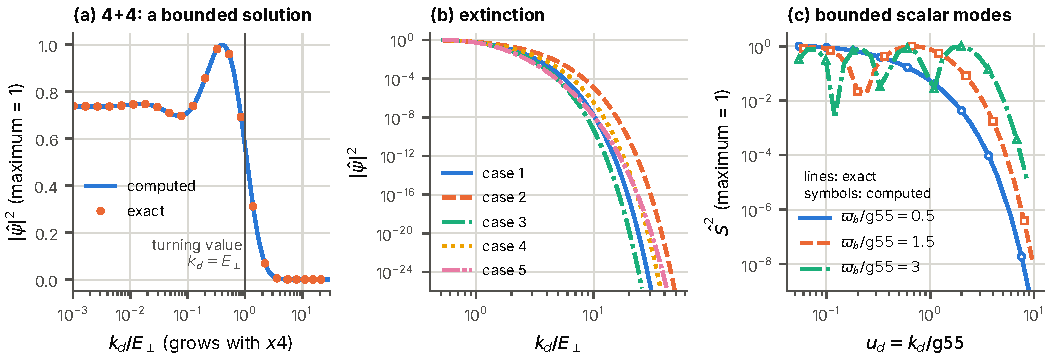
\includegraphics[width=\textwidth]{fig_extinction}
\caption{\label{fig:extinction}Extinction on the deflating $4{+}4$ spacetime. (a) A bounded solution:
$|\hpsi|^{2}$ against the physical wavenumber $\kd/\Eperp$, which grows with the time; computed
(line) and the exact form (\ref{eq:magnitude}) (symbols). It is constant long before the crossing at
$\kd=\Eperp$ and falls after it. (b) Five cases, with one, two or three wavenumbers $k_t$ different
from zero and with equal and unequal rates, on a logarithmic scale. (c) The bounded modes of the
Vorton-Scalar on the same spacetime (Sec.~\ref{sec:scalarmodes}), which are extinguished in the same
way; lines: exact, symbols: computed.}
\end{figure*}

\emph{The law of the extinction.} In the semiclassical (WKB) approximation the bounded solution
falls beyond the turning value, at which $\kd=\Eperp$, as $e^{-\Swkb}$ with
\begin{align}
\Swkb&=\int_{x4_{\mathrm{turn}}}^{x4}\sqrt{\kd^{2}-\Eperp^{2}}\;dx4'\nonumber\\
&=\frac{1}{\rt}\Big[\sqrt{\kd^{2}-\Eperp^{2}}-\Eperp\arccos\frac{\Eperp}{\kd}\Big],
\label{eq:Swkb}
\end{align}
which approaches $(\kd-\tfrac{\pi}{2}\Eperp)/\rt$ for $\kd\gg\Eperp$. The exact solution fixes the
constant that the approximation leaves open:
\begin{equation}
\begin{aligned}
\ln\frac{|\hpsi|_{\mathrm{early}}}{|\hpsi|_{\mathrm{late}}}-\Swkb\ \longrightarrow\ {}&\tfrac12\ln2\\
&-\tfrac12\ln\big(1+e^{-2\pi\Eperp/\rt}\big).
\end{aligned}
\label{eq:constant}
\end{equation}

The numerical solution of Eq.~(\ref{eq:K}) for all sixteen components confirms these statements
(Fig.~\ref{fig:extinction}). Beyond the turning value exactly eight of the sixteen solutions stay
bounded; followed backwards to early times they contain parts of positive and of negative frequency
of equal weight, to $2\times10^{-14}$. Where one rate governs, the computed magnitude equals
Eq.~(\ref{eq:magnitude}) over the range $0.02<\ud<12$ to a relative deviation of
$3.6\times10^{-12}$, and Eq.~(\ref{eq:constant}) holds to $3.6\times10^{-4}$ at $\Swkb=30$. With
three unequal rates no exact solution is known; the bounded solutions fall as $e^{-\Swkb}$ times a
factor that depends on the internal state, with a spread of 0.40 in its logarithm at $\Swkb=30$.

\subsection{What the result means}

On the flat $4{+}4$ spacetime a field that depends on the additional times evolves non-unitarily in
the ordinary time. This is the principal difficulty of four time-like dimensions
\cite{Tegmark1997,CraigWeinstein2009}; on flat spacetime it can only be met by imposing that the
fields do not depend on those times. On the deflating $4{+}4$ spacetime every admissible mode
that depends on a deflating time is a standing wave that is extinguished after its crossing, with an
exponent $\Swkb$ that grows as $e^{\rt\,x4}$. What remains at late times is the sector of fields
that do not depend on $x5,x6,x7$, and in that sector the evolution is unitary and
$\hpsi^\dagger\hpsi$ is conserved. \emph{The deflation of the three additional times removes,
dynamically, the sector that causes the difficulty.} The classical counterpart is the turning value
of Sec.~\ref{sec:geodesics}.

The limits of this conclusion must be stated with equal clarity. The eight growing solutions are
discarded because they are unbounded. That is a condition of admissibility, imposed as in the theory
of a potential barrier; it is not derived from a principle. The theory still has no positive
conserved charge for modes that depend on the deflating times, and a consistent quantization exists,
as before, only for the sector that does not depend on them. What has been shown is that the
admissible modes outside that sector die out, not that the difficulty of four time-like dimensions
has been solved.

\subsection{The numerical method}

The equations of this section are linear, with coefficients that grow exponentially, and an
integrator with a fixed step fails on them. The program uses a commutator-free Magnus method of the
fourth order: over each step the solution is advanced by the product of two matrix exponentials of
linear combinations of the coefficient matrix at two Gauss points. Because the square of
$K$ is a multiple of the unit matrix at any one time, each exponential is evaluated in
closed form. The length of a step is chosen so that
neither the phase accumulated in it nor the relative change of the coefficients exceeds a fixed
bound. An independent program,
which uses an explicit Runge-Kutta method of the eighth order and the Bessel functions of another
library, confirms Eq.~(\ref{eq:exact}) and, to the accuracy of the semiclassical form at the
exponent that it reaches, Eq.~(\ref{eq:constant}) (Appendix~\ref{app:checks}).

\section{The Vorton-Scalar and the deflation clock}
\label{sec:clock}

\subsection{The model}

The model contains, besides the fermion field, a complex scalar field, the \emph{Vorton-Scalar}
$\PhiVS$, whose vacuum value gives the fermions a mass and whose exchange binds two fermions into a
pair. This subsection states the complete model on the deflating spacetime: the fermion field with a
mass term and with the self-interaction of Sec.~\ref{sec:dirac}, and the Vorton-Scalar. The
Vorton-Scalar brings three real, positive constants: its self-coupling $\lamVS$, the constant
$\vVS$ that fixes the magnitude $\vVS/\sqrt2$ at which the potential of the scalar is lowest, and
its Yukawa coupling $\yVS$ to the fermions. The fermion field brings the mass $m_D$ of its
Lagrangian, called the \emph{bare Dirac mass} from here on, and the couplings $g_r$ of its
self-interaction. The chirality matrix is denoted by $\chi$, with
$\chi=\gamma^{0}\gamma^{1}\cdots\gamma^{7}$, which is real on the $4{+}4$ spacetime,
and the chiral projectors are $P^{L,R}=\tfrac12(1\mp\chi)$.

On a curved spacetime a Lagrangian is multiplied by the volume factor $\Vd$, derivatives of spinors
become covariant derivatives, and the flat metric is replaced by the curved one.
On the $4{+}4$ spacetime the Yukawa coupling can be written only in the sector of fields that do not
depend on the additional times, the quantized sector of Sec.~\ref{sec:forms}, because only there
does the adjoint $\bar\psi=\psi^\dagger\beta$ exist with which the chiral projectors combine into
a real, invariant term; the model is defined there. (The covariant adjoint cannot serve in the Yukawa
coupling: $\Cm$ commutes with $\chi$, so that $\tilde\psi\psi$ and $\tilde\psi\chi\psi$ are each
invariant under the chiral transformation and do not rotate into each other, whereas a complex
scalar field whose phase is the Goldstone mode of that transformation must couple to two bilinears
that do, $\bar\psi\psi$ and $\bar\psi\,i\chi\,\psi$. The Yukawa coupling is therefore written with
$\bar\psi$ whatever the form of the self-interaction, and an expectation value of the scalar shifts
the masses of both halves of the field by the same amount.) On the deflating spacetime Sec.~\ref{sec:modes}
gives that sector a dynamical reason. In it the model is
\begin{align}
\mathcal L_{\tg}^{\mathrm{VS}}={}&\hpsi^\dagger\big(i\partial_4+i\sum_{j=0}^{3}\alpha^{j}\partial_j-\beta\,m_D\big)\hpsi+\Vd\,\Lself\nonumber\\
&+\Vd\,\Big[|\partial_4\PhiVS|^{2}-\sum_{j=0}^{3}|\partial_j\PhiVS|^{2}\Big]\nonumber\\
&-\Vd\,\lamVS\Big(|\PhiVS|^{2}-\frac{\vVS^{2}}{2}\Big)^{2}\nonumber\\
&-\Vd\,\yVS\,\bar\psi\big(\PhiVS\,P^{R}+\PhiVS^{*}\,P^{L}\big)\psi ,
\label{eq:LVS}
\end{align}
with the Hermitian matrices $\beta=-i\gamma^{4}$ and $\alpha^{j}=-\gamma^{4}\gamma^{j}$,
$\bar\psi=\psi^\dagger\beta$, and the self-interaction $\Lself=\LselfC$ of form C,
Eq.~(\ref{eq:LselfC}), the definition (with $\LselfQ$ of Eq.~(\ref{eq:LselfQ}) in its place the model
is that of the alternative form Q). The first line is the positive Lagrangian (\ref{eq:Lpos}) for the weighted field
$\hpsi=\sqrt{\Vd}\,\psi$, with the bare Dirac mass, and the self-interaction; without the
self-interaction its equation of motion is the covariant Dirac equation (\ref{eq:dirac}) in this
sector. The other terms carry the volume factor.
The Lagrangian is invariant under the phase transformation $\psi\to e^{i\epsilon}\psi$ of the
fermion number, $U(1)_F$, whatever its constants are. Without the bare Dirac mass, and with a
self-interaction that satisfies the condition (\ref{eq:chiralcond}), it is also invariant under the
chiral transformation $\UVS$: $\psi\to e^{i\epsilon\chi}\psi$ with
$\PhiVS\to e^{-2i\epsilon}\PhiVS$. These statements hold on the deflating spacetime as on flat
spacetime, because the transformations do not involve the coordinates. \emph{The case $m_D=0$,
$g_r=0$ is the model in which the whole mass of the fermions comes from the Vorton-Scalar and the
whole interaction from its exchange;} Secs.~\ref{sec:gap} to \ref{sec:order} treat it first, and
Secs.~\ref{sec:ks}, \ref{sec:gapcontact} and \ref{sec:cjtcontact} then add the bare mass and the
self-interaction and say what each changes.

A constant field $\PhiVS=\vVS/\sqrt2$ with $\psi=0$ solves the field equations on the deflating
spacetime, because a constant has no derivatives: the vacuum value is the same at all times. It
breaks $\UVS$. Around it the Vorton-Scalar has two modes: the \emph{radial mode}, a real field of the
mass $m_s$, and the \emph{phase mode}, a real massless field, the Goldstone boson of the broken
symmetry (massless if $\UVS$ is exact; Sec.~\ref{sec:cjtcontact} computes the mass that a bare Dirac
mass gives it). The fermions acquire the mass $m=m_D+m_Y$, of which $m_Y=\yVS\vVS/\sqrt2$ comes from
the Vorton-Scalar. Both modes couple to the fermions with the same strength
$\gVS$, the radial mode to the scalar density $\bar\psi\psi$ and the phase mode to the pseudoscalar
density $\bar\psi\,i\chi\,\psi$:
\begin{equation}
\begin{aligned}
m_Y&=\frac{\yVS\,\vVS}{\sqrt2},&\qquad m_s&=\sqrt{2\lamVS}\,\vVS,\\
\gVS&=\frac{m_Y}{\vVS},&\qquad\aVS&=\frac{\gVS^{2}}{4\pi}.
\end{aligned}
\label{eq:masses}
\end{equation}

\subsection{Fields that do not depend on the extra coordinates}

Consider fields that do not depend on the four extra coordinates
$x0,x5,x6,x7$, and introduce the weighted fields
\begin{equation}
\hpsi=\sqrt{\Vd}\,\psi,\qquad\hat\Phi_{\mathrm{VS}}=\sqrt{\Vd}\,\PhiVS .
\end{equation}
Each term of Eq.~(\ref{eq:LVS}) is rewritten in turn. The kinetic term and the mass term of the
fermions are the flat ones for $\hpsi$ (Sec.~\ref{sec:dirac}). The self-interaction contains four
fermion fields and therefore the factor $\Vd\cdot\Vd^{-2}$, as in Eq.~(\ref{eq:grun}). The Yukawa
term contains one scalar and two fermion fields
and therefore the factor $\Vd\cdot\Vd^{-3/2}$. The potential becomes
$(\lamVS/\Vd)\,(|\hat\Phi_{\mathrm{VS}}|^{2}-\Vd\vVS^{2}/2)^{2}$. In the kinetic term of the scalar the
derivative along the time acts on the weight as well,
$\sqrt{\Vd}\,\partial_4\PhiVS=\partial_4\hat\Phi_{\mathrm{VS}}+\tfrac12\gsum\,\hat\Phi_{\mathrm{VS}}$,
which gives a term $\tfrac14\gsum^{2}|\hat\Phi_{\mathrm{VS}}|^{2}$ and a total derivative. The result
is the flat Lagrangian for the weighted fields, with four replacements and one additional term:
\begin{equation}
\begin{aligned}
&\yVS\to\frac{\yVS}{\sqrt{\Vd(x4)}},\qquad\lamVS\to\frac{\lamVS}{\Vd(x4)},\qquad g_r\to\frac{g_r}{\Vd(x4)},\\
&\vVS\to\vVS\sqrt{\Vd(x4)},\qquad\text{and }+\frac{\gsum^{2}}{4}\,|\hat\Phi_{\mathrm{VS}}|^{2}.
\end{aligned}
\label{eq:couplings}
\end{equation}
The bare Dirac mass $m_D$ is not replaced. With a constant volume of the extra coordinates the same
replacements define the couplings of a four-dimensional description on flat spacetime. Here that
volume is the coordinate volume of a cell times $\Vd(x4)$, and it shrinks. The additional term lowers the square of
the mass of each mode of the scalar by $\gsum^{2}/4$ in the equation of the weighted field;
Section~\ref{sec:scalarmodes} shows what it does. From here on the couplings $\yVS$, $\lamVS$,
$\vVS$, $\gVS$, $\aVS$ and $g_r$ are those of the four-dimensional description at the time
considered.

\subsection{The deflation clock}

Define the \emph{deflation clock}
\begin{equation}
\td=\gsum\,(x4-x4_{\mathrm{ref}}),
\label{eq:clock}
\end{equation}
the number of e-foldings by which the volume $\Vd$ has shrunk since a reference time
$x4_{\mathrm{ref}}$, which is chosen in each application. By Eq.~(\ref{eq:couplings}) every quantity
of the four-dimensional description is proportional to $e^{n\td}$ with a definite exponent $n$
(Table~\ref{tab:exponents}). Three observations organize what follows.

\begin{table*}
\caption{\label{tab:exponents}How the quantities of the four-dimensional description follow the
deflation clock: each is proportional to $e^{n\td}$. The last two rows hold under additional
assumptions, which Secs.~\ref{sec:cosmo} and \ref{sec:higgs} state and examine.}
\begin{ruledtabular}
\begin{tabular}{p{0.37\textwidth}p{0.47\textwidth}c}
quantity & meaning & exponent $n$ \\
\hline
$V_d$ & $b_5b_6b_7$: the factor $\sqrt{\lvert\det g\rvert}$ of the measure & $-1$ \\
$y_{\mathrm{VS}}$ of the four-dimensional description & Yukawa coupling of the weighted fields & $\tfrac12$ \\
$\lambda_{\mathrm{VS}}$ of the four-dimensional description & quartic coupling of the weighted Vorton-Scalar & $1$ \\
$v_{\mathrm{VS}}$ of the four-dimensional description & vacuum value of the weighted Vorton-Scalar & $-\tfrac12$ \\
$m_D$ & bare Dirac mass (the mass term of the Lagrangian of the fermion field) & $0$ \\
$m_Y$ & part of the fermion mass that the Vorton-Scalar gives, $y_{\mathrm{VS}}v_{\mathrm{VS}}/\sqrt2$; the mass in vacuum is $m=m_D+m_Y$ & $0$ \\
$m_s$ & mass of the radial mode $\sqrt{2\lambda_{\mathrm{VS}}}\,v_{\mathrm{VS}}$ & $0$ \\
$g_r$ of the four-dimensional description & each of the nine couplings of the self-interaction of the weighted field, and with them the mean-field couplings $G_S$, $G_V$ & $1$ \\
$g_{\mathrm{VS}}$ & coupling of both modes of the Vorton-Scalar to the fermions, $m_Y/v_{\mathrm{VS}}$ & $\tfrac12$ \\
$\alpha_{\mathrm{VS}}$ & $g_{\mathrm{VS}}^2/4\pi$ & $1$ \\
$G_{\mathrm{VS}}$ & constant of the Fermi type of the neutral-current interaction, $1/(\sqrt2\,v_{\mathrm{VS}}^2)$ & $1$ \\
$D_{\mathrm{VS}}$ & $\alpha_{\mathrm{VS}}\,m/m_s$: decides whether two fermions bind & $1$ \\
$C$ & $g_{\mathrm{VS}}^2m^2/m_s^2$: decides the state of matter & $1$ \\
$m_\vartheta$ & mass of the phase mode of the Vorton-Scalar when $m_D\neq0$, $m_\vartheta^2v_{\mathrm{VS}}^2=\lvert\langle\bar\psi\psi\rangle_{\mathrm{vac}}\rvert\,m_Dm_Y/m$ & $\tfrac12$ \\
vortex energy per length & proportional to $v_{\mathrm{VS}}^2$ (four-dimensional) & $-1$ \\
$G_{\mathrm{Fermi}}$ (Fermi constant of the weak interaction) if the vacuum value of the Vorton-Scalar sets the electroweak scale (assumption HV) & $1/(\sqrt2\,v_{\mathrm{VS}}^2)$, four-dimensional vacuum value & $1$ \\
$G_N$ (Newton's constant) if gravity is eight-dimensional (A2) & $G_8$ divided by the volume of $x5,x6,x7$ & $1$ \\
\end{tabular}
\end{ruledtabular}
\end{table*}

\emph{The masses do not change.} The bare Dirac mass is not affected at all, and the part $m_Y$ of
the fermion mass and the mass $m_s$ of the radial mode contain the couplings in combinations from
which the volume cancels. So do the Fermi momentum and the Fermi
energy of matter with a given number of particles per unit of ordinary volume.

\emph{The couplings grow.} The coupling $\gVS=m_Y/\vVS$ grows as $e^{\td/2}$, because the
four-dimensional vacuum value falls. The strength of the attraction, $\aVS$, grows as $e^{\td}$: it
doubles every time the volume of the deflating coordinates halves. Every coupling $g_r$ of the
self-interaction, and with them the couplings $\GS$, $\GV$ of Sec.~\ref{sec:ks}, grows as $e^{\td}$
as well: \emph{the contact interaction and the exchange of the Vorton-Scalar keep their ratio.}

\emph{The two numbers that decide the state of matter grow at the same rate.} These are
\begin{equation}
\DVS=\aVS\,\frac{m}{m_s},\qquad C=\frac{\gVS^{2}m^{2}}{m_s^{2}} .
\label{eq:DC}
\end{equation}
The first decides whether two fermions form a bound pair (Sec.~\ref{sec:pair}), the second whether
matter keeps its fermion mass (Sec.~\ref{sec:cjt}). Their ratio $C/\DVS=4\pi\,m/m_s$ is fixed.

On flat spacetime the model is specified by the masses and the couplings. On a deflating spacetime
it is specified by the masses and the values of the couplings \emph{at one time}; the deflation then
carries it through all larger couplings. The constants of the flat theory become functions of the
time, and its thresholds are passed one after another (Fig.~\ref{fig:clock}).

\begin{figure*}
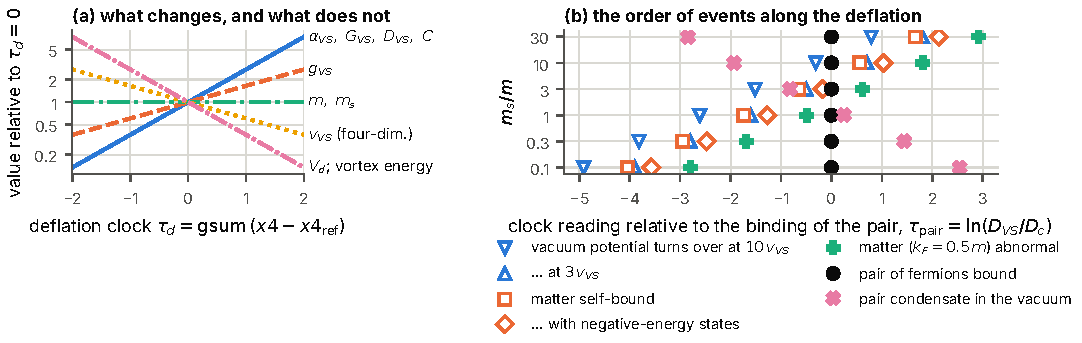
\includegraphics[width=0.9\textwidth]{fig_clock}
\caption{\label{fig:clock}The deflation clock. (a) How the quantities of the four-dimensional
description change with the clock $\td$ (logarithmic scale; values relative to $\td=0$). (b) The
order of events along the deflation for six ratios $m_s/m$: the clock reading of each event relative
to the moment at which two fermions form a bound pair (Table~\ref{tab:events}).}
\end{figure*}

\subsection{Modes of the Vorton-Scalar}
\label{sec:scalarmodes}

Let $\varphi_{\mathrm{bos}}$ stand for the radial mode or the phase mode, with the mass
$m_{\mathrm{bos}}=m_s$ or $m_{\mathrm{bos}}=0$. To first order in the field, a mode with a wavenumber
of the magnitude $k$ along the flat coordinates and the wavenumbers $k_t$ along the deflating ones
obeys
\begin{equation}
\begin{aligned}
&\frac{1}{\Vd}\,\partial_4\big(\Vd\,\partial_4\varphi_{\mathrm{bos}}\big)\\
&\quad+\Big(k^{2}-\sum_t\frac{k_t^{2}}{b_t^{2}}+m_{\mathrm{bos}}^{2}\Big)\varphi_{\mathrm{bos}}=0 .
\end{aligned}
\label{eq:scalar}
\end{equation}
The wavenumbers along the deflating coordinates, which are time-like, enter with the sign
opposite to that of $k^{2}$, as for the fermions.

\emph{Modes that do not depend on the deflating coordinates.} With $k_t=0$ the equation has constant
coefficients, and its solutions are the exponentials
\begin{equation}
\varphi_{\mathrm{bos}}\propto\exp\Big\{\Big[\frac{\gsum}{2}\pm\sqrt{\frac{\gsum^{2}}{4}-k^{2}-m_{\mathrm{bos}}^{2}}\,\Big]x4\Big\}.
\label{eq:exponents}
\end{equation}
If $k^{2}+m_{\mathrm{bos}}^{2}>\gsum^{2}/4$, the mode oscillates with the frequency
$\varpi_b=(k^{2}+m_{\mathrm{bos}}^{2}-\gsum^{2}/4)^{1/2}$, and its amplitude grows as
$e^{\gsum\,x4/2}$. The growth is that of the weight alone: the weighted field has a constant
amplitude, and the number of quanta in a cell of fixed coordinates is conserved while the cell
shrinks. Otherwise the mode does not oscillate. For the radial mode this never happens if
$m_s>\gsum/2$, which holds by many orders of magnitude for any rate that observation allows
(Sec.~\ref{sec:cosmo}). For the phase mode it happens at wavelengths longer than $4\pi/\gsum$. At
$k=0$ the two exponents of the phase mode are $0$ and $\gsum$: a constant phase, which costs nothing,
and a phase that advances at a rate proportional to $1/\Vd$, which is the conservation of the charge
of $\UVS$ in a shrinking volume. Neither is an instability of the vacuum. Figure~\ref{fig:scalar}
shows the exponents.

\begin{figure*}
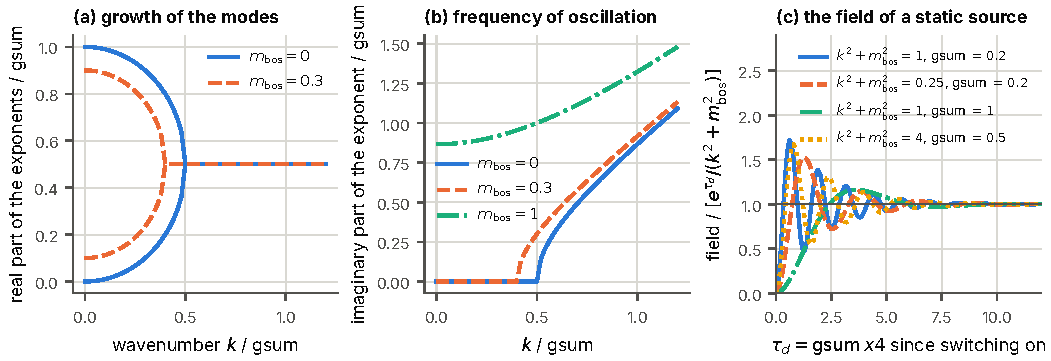
\includegraphics[width=\textwidth]{fig_scalar}
\caption{\label{fig:scalar}Modes of the Vorton-Scalar that do not depend on the deflating
coordinates. (a) Real parts of the two exponents of Eq.~(\ref{eq:exponents}) against the wavenumber,
for the phase mode and for a radial mode, in units of $\gsum$. (b) Their imaginary part, the
frequency of oscillation. (c) The field that a static source builds up from zero, divided by the form
$e^{\td}/(k^{2}+m_{\mathrm{bos}}^{2})$ that leads to Eq.~(\ref{eq:yukawa}).}
\end{figure*}

\emph{The potential between two fermions.} Two fermions at rest attract each other by exchanging the
radial mode. The density of a fixed number of fermions grows as $1/\Vd$, so that the radial mode
obeys Eq.~(\ref{eq:scalar}) with a source proportional to $e^{\gsum\,x4}$. The solution that follows
the source is $e^{\gsum\,x4}/(k^{2}+m_{\mathrm{bos}}^{2})$ times the source, as substitution shows:
the terms $\gsum^{2}-\gsum\cdot\gsum$ cancel, and the denominator contains the \emph{unshifted} mass.
The potential between two fermions at rest is therefore, at every moment, a Yukawa potential,
\begin{equation}
V_s(r)=-\aVS(x4)\,\frac{e^{-m_sr}}{r},
\label{eq:yukawa}
\end{equation}
with the range $1/m_s$ unchanged and the strength of the moment. The numerical solution from rest
approaches this form with a transient that decays as $e^{-\td/2}$ [Fig.~\ref{fig:scalar}(c)]; after
$\td=20$ the relative difference is below $4\times10^{-5}$ in the four cases computed.

\emph{Modes that depend on a deflating coordinate.} For $k_t\ne0$ the weighted field obeys
$\partial_4^{2}\hat\varphi_{\mathrm{bos}}+(\varpi_b^{2}-\kd^{2})\,\hat\varphi_{\mathrm{bos}}=0$
with the physical wavenumber $\kd$ of Eq.~(\ref{eq:kd}), and the scalar behaves as the fermion field
does.
Beyond the turning value, at which $\kd=\varpi_b$, one solution decays and one grows. The bounded
solution is the modified Bessel function of the imaginary order $i\varpi_b/\rt$ that decays at large
argument. At early times it is a standing wave; at late times it falls as $e^{-\ud}$
(Fig.~\ref{fig:extinction}). The scalar field, like the fermion field, loses its dependence on the
deflating times.

\section{Matter: the Kohn-Sham analysis}
\label{sec:ks}

This section determines the states of uniform matter made of the fermions of the model when the
self-interaction acts between them. The Vorton-Scalar is set aside here ($\yVS=0$, so that the mass
$m$ of the fermions in vacuum is the bare Dirac mass); Sec.~\ref{sec:cjtcontact} restores it.

\subsection{The method}
\label{sec:ksmethod}

In the method of Kohn and Sham \cite{KohnSham1965} a system of interacting fermions is replaced by
independent fermions that move in fields which their own densities determine. The energy is written
as a function of the densities; the fields are its derivatives; and the densities are computed from
the occupied states in those fields, until both agree. The method is set out here for matter of
one kind of particle, whose densities are two numbers: the number density $n=\langle\psi^\dagger\psi\rangle$
and the scalar density $\nS=\langle\bar\psi\psi\rangle$. (Section~\ref{sec:ksreduced} treats the
two halves of the field together.) The interaction energy is
$\tfrac12\GV n^{2}+\tfrac12\GS\nS^{2}$ with a scalar coupling $\GS$ and a vector coupling $\GV$, and
each particle obeys the Dirac equation with the Hamiltonian matrix
\begin{equation}
\begin{aligned}
\hh_{\mathrm{KS}}&=\sum_j\alpha^{j}k_j+\beta\,\mst+V_0,\\
\mst&=m+\GS\,\nS,\qquad V_0=\GV\,n .
\end{aligned}
\label{eq:hKS}
\end{equation}
The scalar field changes the mass of the particles in matter from $m$ to $\mst$; the vector field
shifts all energies by $V_0$. A negative $\GS$ is an attraction (it lowers the mass and the energy)
and a positive $\GV$ a repulsion; this is the structure of the mean-field theory of dense matter
with a scalar and a vector field \cite{Walecka1974}. With the couplings of Eq.~(\ref{eq:GHF}) the exchange terms are
contained exactly, because for a contact interaction they are a function of the same two densities.

A particle of the momentum $\vec k$ has the energy $E^{*}(k)+V_0$ with
$E^{*}(k)=(k^{2}+\mstq)^{1/2}$. The occupied states are those with $|\vec k|<\kF$, $\nu$ for each
momentum ($\nu=8$ if all eight internal states of a particle are filled, $\nu=4$ if the particles of
one half of the field are present alone), and averages over them are written
$\langle f\rangle=\nu\int d^{D}k\,f/(2\pi)^{D}$, where $D$ is the number of space dimensions in which
the particles have momentum. Then
\begin{equation}
n=\langle1\rangle=\frac{\nu\,V_D\,\kF^{D}}{(2\pi)^{D}},\qquad\nS=\Big\langle\frac{\mst}{E^{*}}\Big\rangle,
\label{eq:densities}
\end{equation}
with the volume $V_D=\pi^{D/2}/\Gamma_{\mathrm E}(D/2+1)$ of the unit ball ($\Gamma_{\mathrm E}$ is
Euler's gamma function). The second of Eqs.~(\ref{eq:hKS}) with the second of
Eqs.~(\ref{eq:densities}) is the \emph{gap equation} for $\mst$. The energy density is
\begin{equation}
\varepsilon=\langle E^{*}\rangle+\tfrac12\GV\,n^{2}-\frac{(\mst-m)^{2}}{2\GS},
\label{eq:epsKS}
\end{equation}
which is the kinetic and mass energy of the particles plus the interaction energy [the first term
counts the mass as $\mst$ instead of $m$, which the last term corrects]; it is stationary with
respect to $\mst$ exactly when the gap equation holds. The pressure along the coordinate $xj$ is
\begin{equation}
p_j=\Big\langle\frac{k_j^{2}}{E^{*}}\Big\rangle+\pint,\qquad\pint=\tfrac12\GV\,n^{2}+\frac{(\mst-m)^{2}}{2\GS}.
\label{eq:pKS}
\end{equation}
The first term is the momentum that the particles carry across a surface; the \emph{interaction
pressure} $\pint$ is the same in all directions. \emph{Along a coordinate on which the fields do not
depend the particles have no momentum, and the pressure is $\pint$ alone}; this remark is used for
the deflating coordinates below. The chemical potential is $\mu=E^{*}(\kF)+V_0$, and for an
isotropic state $p=\mu n-\varepsilon$. Matter is \emph{self-bound} if its energy per particle,
$\varepsilon/n$, is below the mass $m$ at some density; the density at which $\varepsilon/n$ is
smallest is the \emph{saturation} density, where the pressure vanishes and
$\mu=\varepsilon/n$ \cite{HugenholtzVanHove1958}.

Two limitations are stated here once. The filled states of negative energy are not counted (the
\emph{no-sea approximation}); Sec.~\ref{sec:cjtcontact} counts them. And the state is the one of
lowest energy among the solutions of the gap equation: without the filled negative-energy states the
energy as a function of an unrestricted trial mass has no lowest value, because a large negative
trial mass places particles in states of negative rest energy.


\subsection{Fields that do not depend on the deflating coordinates}
\label{sec:ksreduced}

On the $4{+}4$ spacetime matter exists only in the quantized sector: a mode that depends on a
deflating time is extinguished (Sec.~\ref{sec:modes}). The particles then have momentum along
$x0,\dots,x3$, so that $D=4$, or, if the fields do not depend on the hidden coordinate $x0$ either,
along ordinary space, $D=3$. By Eq.~(\ref{eq:couplings}) the equations of flat spacetime hold for the
weighted field at each moment with the couplings of that moment: every coupling $g_r$, and with it
every mean-field coupling of Sec.~\ref{sec:hf}, grows as $e^{\td}$, while the mass $m$ and the
density of particles per unit of the volume of $x0,\dots,x3$ do not change. The ratios of the
couplings are fixed. The deflation therefore carries the matter through a one-parameter sequence of
interactions of growing strength.

\emph{The equations of two halves.} The field has two halves (Sec.~\ref{sec:forms}), and the
interaction energy (\ref{eq:EHF}) depends on the densities of both. The particles of the half
$\Wg=\pm1$ have the mass $\mstpm$ and the energy shift $V_{0\pm}$,
\begin{equation}
\begin{aligned}
\mstpm&=m+\GStot\,\nS\pm\GSdif\,n_{SW},\\
V_{0\pm}&=\GVtot\,n\pm\GVdif\,n_W ,
\end{aligned}
\label{eq:hKShalves}
\end{equation}
and fill the states up to the Fermi momenta $k_{F\pm}$, four for each momentum. With
$E^{*}_\pm(k)=(k^{2}+m_\pm^{*2})^{1/2}$,
\begin{equation}
\begin{aligned}
n_\pm&=4\!\int_{|\vec k|<k_{F\pm}}\!\frac{d^{D}k}{(2\pi)^{D}},\\
n_{S\pm}&=4\!\int_{|\vec k|<k_{F\pm}}\!\frac{d^{D}k}{(2\pi)^{D}}\,\frac{\mstpm}{E^{*}_\pm},
\end{aligned}
\label{eq:denshalves}
\end{equation}
\begin{equation}
\begin{aligned}
\varepsilon={}&\sum_\pm4\!\int_{|\vec k|<k_{F\pm}}\!\frac{d^{D}k}{(2\pi)^{D}}\,E^{*}_\pm
+\tfrac12\big(\GVtot\,n^{2}+\GVdif\,n_W^{2}\big)\\
&-\tfrac12\big(\GStot\,\nS^{2}+\GSdif\,n_{SW}^{2}\big),
\end{aligned}
\label{eq:epshalves}
\end{equation}
and the pressure along $x0,\dots,x3$ is the sum of the kinetic terms of Eq.~(\ref{eq:pKS}) for the two
halves and of the interaction pressure
$\pint=\tfrac12(\GVtot n^{2}+\GVdif n_W^{2})+\tfrac12(\GStot\nS^{2}+\GSdif n_{SW}^{2})$, which is the
whole pressure along the deflating coordinates. The first of Eqs.~(\ref{eq:hKShalves}) with the second
of Eqs.~(\ref{eq:denshalves}) are two coupled gap equations for $m^{*}_+$ and $m^{*}_-$. If one half is
empty, or if both halves are equally filled, these equations are those of Sec.~\ref{sec:ksmethod} for
one kind of particle: with $\nu=4$ and the couplings $\GSsame$, $\GVsame$ for one filled half, and
with $\nu=8$ and the couplings $\GStot$, $\GVtot$ for equal halves. Because the interaction can move
two particles from one half to the other (Sec.~\ref{sec:forms}), the numbers of the two halves are not
fixed separately: at a given total density $n$ the state is the one of lowest energy with respect to
the \emph{polarization}
\begin{equation}
\mathrm{pol}_W=\frac{n_+-n_-}{n},
\label{eq:pol}
\end{equation}
between 0 (equal halves) and 1 (one half filled; the sign is free by the symmetry between the
halves). Among the solutions of the gap equations those with non-negative masses are taken, which
continue the dilute gas. Such a solution is a regular function of the density and of the couplings
while the eigenvalues of the matrix $\mathsf R_{\mathrm{gap}}$ of the derivatives of the right-hand
sides of the two gap equations with respect to the two masses stay below 1; they are
$2\,\GStot\,\partial n_{S+}/\partial m^{*}_+$ and $2\,\GSdif\,\partial n_{S+}/\partial m^{*}_+$ for equal
halves, and $\GSsame\,\partial n_{S+}/\partial m^{*}_+$ and 0 for one filled half.

The numbers below are given for two sets of couplings of the Lagrangian, each with one strength
$g>0$ that grows as $e^{\td}$: \emph{set A}, a scalar attraction alone, $g_0=-g$; and \emph{set B},
$g_0=-g$ with a vector repulsion one tenth as large, $g_1=+0.1\,g$; all other couplings zero. For
these Table~\ref{tab:kscoup} gives the mean-field couplings of Eqs.~(\ref{eq:EHF}) and
(\ref{eq:Esame}).

\begin{table*}
\caption{\label{tab:kscoup}The mean-field couplings of the two halves of the field for the sets A
and B of couplings of the Lagrangian, in the two forms, in units of the strength $g$ (exact).}
\begin{ruledtabular}
\begin{tabular}{cccccccccc}
set & form & $\GVtot$ & $\GStot$ & $\GVdif$ & $\GSdif$ & $\GVsame$ & $\GSsame$ & $\GVopp$ & $\GSopp$ \\
\hline
A & C & $\tfrac{1}{16}$ & $\tfrac{1}{16}$ & $\tfrac{1}{16}$ & $-\tfrac{15}{16}$ & $\tfrac{1}{8}$ & $-\tfrac{7}{8}$ & 0 & $1$ \\
A & Q & $\tfrac{1}{16}$ & $-\tfrac{15}{16}$ & $\tfrac{1}{16}$ & $\tfrac{1}{16}$ & $\tfrac{1}{8}$ & $-\tfrac{7}{8}$ & 0 & $-1$ \\
B & C & $\tfrac{1}{16}$ & $\tfrac{1}{20}$ & $\tfrac{1}{5}$ & $-\tfrac{79}{80}$ & $\tfrac{21}{80}$ & $-\tfrac{15}{16}$ & $-\tfrac{11}{80}$ & $\tfrac{83}{80}$ \\
B & Q & $\tfrac{1}{5}$ & $-\tfrac{79}{80}$ & $\tfrac{1}{16}$ & $\tfrac{1}{20}$ & $\tfrac{21}{80}$ & $-\tfrac{15}{16}$ & $\tfrac{11}{80}$ & $-\tfrac{83}{80}$ \\
\end{tabular}
\end{ruledtabular}
\end{table*}

\emph{Form C polarizes matter; form Q does not.} Table~\ref{tab:kspol} and Fig.~\ref{fig:kspol} give
the energy per particle as a function of the polarization, for the same couplings of the Lagrangian
in the two forms. In form C the energy falls with the polarization, in form Q it rises. Over
48 cases (two dimensions, two sets, three strengths, four densities) the state of
lowest energy is polarized in 48 cases in form C and in 0 cases
in form Q. The reason is Eq.~(\ref{eq:Esame}): in form C a particle is attracted by the particles of
its own half ($\GSsame<0$) and repelled by those of the other half ($\GSopp>0$), so that the
particles gather in one half and break the symmetry between the halves spontaneously; in form Q a
particle is attracted by both. (Of the 3936 states examined,
108 states of form Q with unequal halves do not exist as solutions with
non-negative masses, at three and six times the threshold and high density; the states with equal
halves and with one filled half exist in all cases, and in form C every state exists.)

\begin{table*}
\caption{\label{tab:kspol}Energy per particle minus $m$ of matter of the total density of the Fermi
momentum $k_{F,\mathrm{tot}}=0.6\,m$ (the Fermi momentum that the density would have with equal halves),
at three polarizations, in the two forms of the $4{+}4$ model (units $m$). Strength: in units of the
strength at which form Q first binds matter.}
\begin{ruledtabular}
\begin{tabular}{ccccccccc}
$D$ & set & strength & C, $\mathrm{pol}_W=0$ & C, $0.5$ & C, $1$ & Q, $\mathrm{pol}_W=0$ & Q, $0.5$ & Q, $1$ \\
\hline
4 & A & 1.5 & $+0.1358$ & $+0.1155$ & $+0.0598$ & $-0.0159$ & $+0.0016$ & $+0.0598$ \\
4 & A & 3 & $+0.1588$ & $+0.1121$ & $-0.0099$ & $-0.1137$ & $-0.0897$ & $-0.0099$ \\
4 & B & 1.5 & $+0.1436$ & $+0.1187$ & $+0.0543$ & $-0.0343$ & $-0.0138$ & $+0.0543$ \\
4 & B & 3 & $+0.1745$ & $+0.1239$ & $+0.0179$ & $-0.1044$ & $-0.0764$ & $+0.0179$ \\
3 & A & 1.5 & $+0.1264$ & $+0.1074$ & $+0.0553$ & $-0.0380$ & $-0.0158$ & $+0.0553$ \\
3 & A & 3 & $+0.1511$ & $+0.1039$ & $-0.0167$ & $-0.1430$ & $-0.1132$ & $-0.0167$ \\
3 & B & 1.5 & $+0.1301$ & $+0.1107$ & $+0.0612$ & $-0.0406$ & $-0.0164$ & $+0.0612$ \\
3 & B & 3 & $+0.1583$ & $+0.1140$ & $+0.0197$ & $-0.1188$ & $-0.0864$ & $+0.0197$ \\
\end{tabular}
\end{ruledtabular}
\end{table*}

\begin{figure*}
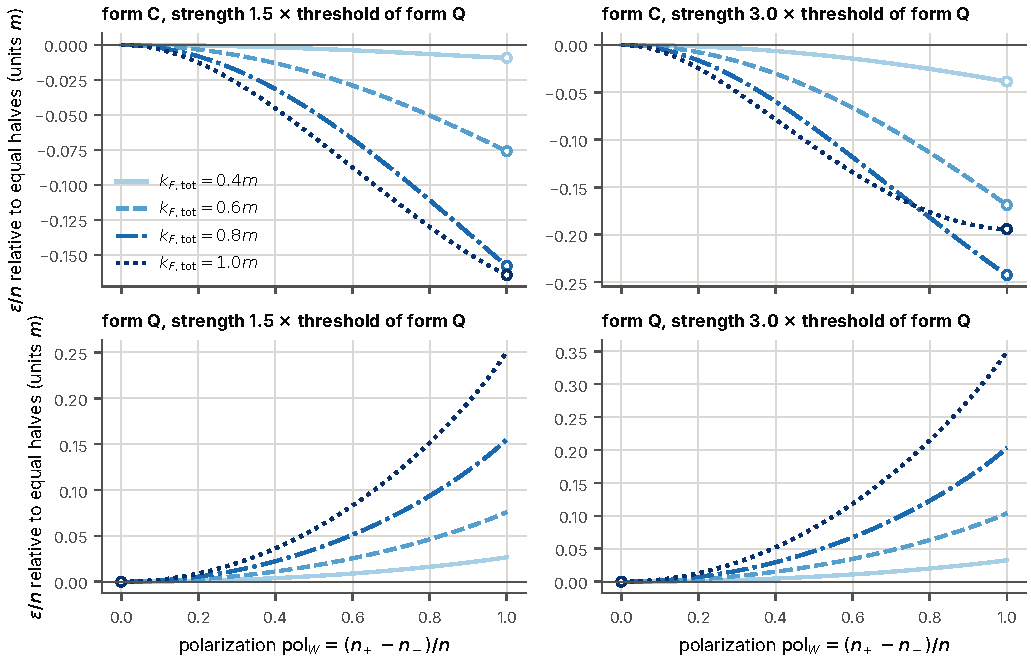
\includegraphics[width=0.86\textwidth]{fig_forms_polarization}
\caption{\label{fig:kspol}Energy per particle of matter of a given total density against the
polarization of the two halves of the field, relative to its value for equal halves ($D=4$, set A).
Upper row: form C; lower row: form Q; left: 1.5 times, right: 3 times the strength at which form Q
first binds matter. The four curves are four total densities; the circle marks the lowest point of
each curve.}
\end{figure*}

\emph{A gas becomes self-bound matter at a definite moment}: when the strength reaches the threshold
of Table~\ref{tab:ksthr}. In form C the bound state has one half filled, in form Q equal halves, in
all eight cases; each threshold agrees with that of matter of one kind (four states with
$\GSsame,\GVsame$, or eight states with $\GStot,\GVtot$) computed by the routines of
Sec.~\ref{sec:ksmethod}, to $5.7\times10^{-14}$. Matter of form C needs
2.74 times (set A) and 2.74 times (set B) the strength of
form Q in $D=4$, and 2.51 and 2.52 times in $D=3$: on the
clock it binds later by $\Delta\td=1.01$ and $1.01$ ($D=4$),
$0.92$ and $0.92$ ($D=3$). Two things make the difference.
Only four of the eight internal states take part. And the attraction inside one half,
$\GSsame=\tfrac78g_0$ for set A, is weaker than the attraction $\GStot=\tfrac{15}{16}g_0$ that matter
of form Q with equal halves feels.

\begin{table*}
\caption{\label{tab:ksthr}The smallest strength $g$ of the couplings of the Lagrangian at which
uniform matter is self-bound, in the two forms of the $4{+}4$ model (units $m=1$), with the state just
above the threshold: its kind, the Fermi momentum $k_{F,\mathrm{tot}}$ that its density would have with
equal halves, and the masses of the particles of the two halves (for an empty half the mass that a
particle of that half would have). Last column: the largest cutoff for which the vacuum is stable at
that strength (Sec.~\ref{sec:sea}).}
\begin{ruledtabular}
\begin{tabular}{ccccccccc}
$D$ & set & form & $g\,m^{D-1}$ & state & $k_{F,\mathrm{tot}}/m$ & $m^{*}_+/m$ & $m^{*}_-/m$ & $\Lambda_{\max}/m$ \\
\hline
4 & A & C & 224.7386 & one half & 0.6140 & 0.5239 & 1.5441 & 0.520 \\
4 & A & Q & 82.1116 & equal halves & 0.8054 & 0.4946 & 0.4946 & 0.727 \\
4 & B & C & 332.2917 & one half & 0.5211 & 0.5625 & 1.4842 & 0.449 \\
4 & B & Q & 121.0858 & equal halves & 0.6792 & 0.5424 & 0.5424 & 0.628 \\
3 & A & C & 24.5717 & one half & 0.5374 & 0.6454 & 1.4053 & 0.463 \\
3 & A & Q & 9.8090 & equal halves & 0.7356 & 0.6276 & 0.6276 & 0.733 \\
3 & B & C & 31.1674 & one half & 0.4635 & 0.6712 & 1.3638 & 0.400 \\
3 & B & Q & 12.3819 & equal halves & 0.6351 & 0.6575 & 0.6575 & 0.635 \\
\end{tabular}
\end{ruledtabular}
\end{table*}

Figure~\ref{fig:ksbind} and Table~\ref{tab:kssat} follow the saturated matter from the moment of
binding on. Its energy per particle falls monotonically and the mass of its particles falls; the
kind of the state does not change (one half filled in form C, equal halves in form Q) at any of the
101 clock readings examined up to five units of the clock after the threshold. Counted from its own
threshold, matter of form C is somewhat less strongly bound than matter of form Q at the same clock
reading. Along the table the largest eigenvalue of $\mathsf R_{\mathrm{gap}}$ is
0.881. Later the saturated state of form Q reaches the eigenvalue 1, at which its
two masses can separate ($D=4$, set A: $\tau_d=6.416$; $D=4$, set B: not before $\tau_d=9$; $D=3$, set A: $\tau_d=5.296$; $D=3$, set B: $\tau_d=7.323$); that of form C does not.

\begin{table*}
\caption{\label{tab:kssat}Self-bound matter in the two forms along the deflation clock, counted for
each case from its own binding threshold: energy per particle of the saturated state minus $m$ at
four clock readings, and the mass of the particles of the filled half or halves and the Fermi
momentum $k_{F,\mathrm{tot}}$ at the clock readings 1 and 3 (units $m$).}
\begin{ruledtabular}
\begin{tabular}{ccccccccccc}
$D$ & set & form & $\td=1$ & $2$ & $3$ & $4$ & $m^{*}$ at 1 & $m^{*}$ at 3 & $k_{F,\mathrm{tot}}$ at 1 & $k_{F,\mathrm{tot}}$ at 3 \\
\hline
4 & A & C & $-0.1092$ & $-0.2079$ & $-0.2913$ & $-0.3597$ & 0.351 & 0.183 & 0.538 & 0.361 \\
4 & A & Q & $-0.1284$ & $-0.2449$ & $-0.3438$ & $-0.4254$ & 0.319 & 0.156 & 0.713 & 0.486 \\
4 & B & C & $-0.0829$ & $-0.1577$ & $-0.2209$ & $-0.2727$ & 0.392 & 0.215 & 0.452 & 0.301 \\
4 & B & Q & $-0.0968$ & $-0.1842$ & $-0.2580$ & $-0.3185$ & 0.371 & 0.199 & 0.592 & 0.395 \\
3 & A & C & $-0.1226$ & $-0.2400$ & $-0.3365$ & $-0.4116$ & 0.373 & 0.157 & 0.502 & 0.308 \\
3 & A & Q & $-0.1424$ & $-0.2801$ & $-0.3945$ & $-0.4844$ & 0.347 & 0.137 & 0.699 & 0.442 \\
3 & B & C & $-0.0940$ & $-0.1835$ & $-0.2567$ & $-0.3133$ & 0.407 & 0.183 & 0.426 & 0.256 \\
3 & B & Q & $-0.1093$ & $-0.2136$ & $-0.2990$ & $-0.3652$ & 0.389 & 0.170 & 0.588 & 0.357 \\
\end{tabular}
\end{ruledtabular}
\end{table*}

\begin{figure*}
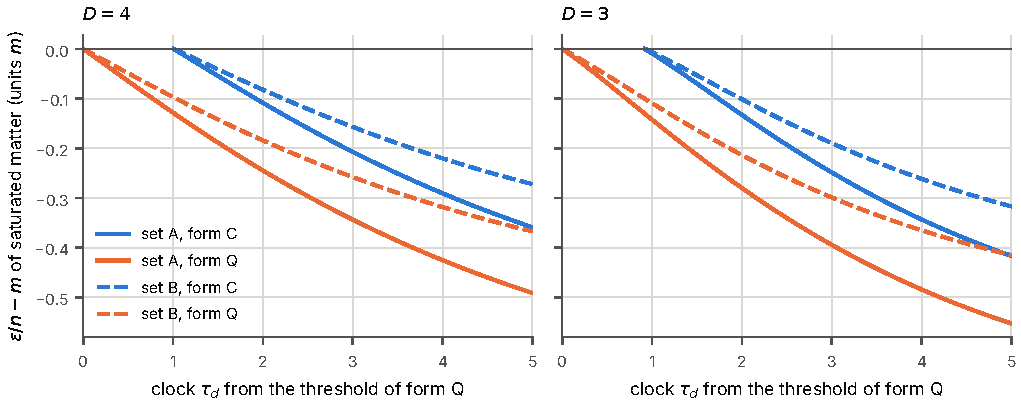
\includegraphics[width=0.86\textwidth]{fig_forms_saturation}
\caption{\label{fig:ksbind}Energy per particle minus the mass of self-bound matter along the deflation
clock, for the same couplings of the Lagrangian in both forms. The clock is counted here from the
moment at which form Q first binds matter of the same set, so that the curves of form C begin later,
where form C first binds. Solid lines: set A; dashed lines: set B; blue: form C (one half filled);
orange: form Q (equal halves). Left: $D=4$; right: $D=3$.}
\end{figure*}

Matter of a \emph{fixed} density is carried through the same sequence (Fig.~\ref{fig:ksgas},
Table~\ref{tab:ksgas}). In form C the two halves become unequal at a definite clock reading before
the binding threshold, and one half is empty at most 0.35 units of the clock later:
the gas polarizes. Its pressure along the flat coordinates becomes negative after the polarization,
or, in 3 of the 8 cases (the higher density), not at all, because the
repulsion $\GVsame$ between the particles of the filled half grows with the couplings while the
attraction saturates as the mass falls. In form Q the halves stay equal and the pressure becomes
negative in all cases: a uniform gas is then unstable against breaking up into drops of saturated
matter. Along the deflating coordinates the pressure is the interaction pressure $\pint$ alone, which
is negative as long as the scalar attraction dominates: \emph{the matter pulls on the deflating
coordinates.} Section~\ref{sec:gravity} uses this.

\begin{table}
\caption{\label{tab:ksgas}A gas of fixed total density in the two forms: the clock readings, counted
from the binding threshold of each case, at which the two halves become unequal, at which one half
is empty, and at which the pressure along the flat coordinates becomes negative. A dash: the event
does not happen for $-3\le\td\le5$.}
\begin{ruledtabular}
\begin{tabular}{ccccccc}
$D$ & set & form & $k_{F,\mathrm{tot}}/m$ & unequal & one half & $p<0$ \\
\hline
4 & A & C & 0.3 & $-0.53$ & $-0.17$ & $+0.31$ \\
4 & A & C & 0.6 & $-1.77$ & $-1.43$ & $-0.43$ \\
4 & A & Q & 0.3 & --- & --- & $+0.78$ \\
4 & A & Q & 0.6 & --- & --- & $-0.36$ \\
4 & B & C & 0.3 & $-0.82$ & $-0.47$ & $+0.06$ \\
4 & B & C & 0.6 & $-1.98$ & $-1.62$ & --- \\
4 & B & Q & 0.3 & --- & --- & $+0.51$ \\
4 & B & Q & 0.6 & --- & --- & $-0.49$ \\
3 & A & C & 0.3 & $-0.93$ & $-0.72$ & $-0.03$ \\
3 & A & C & 0.6 & $-1.48$ & $-1.27$ & --- \\
3 & A & Q & 0.3 & --- & --- & $+0.21$ \\
3 & A & Q & 0.6 & --- & --- & $-0.21$ \\
3 & B & C & 0.3 & $-1.02$ & $-0.88$ & $-0.12$ \\
3 & B & C & 0.6 & $-1.52$ & $-1.32$ & --- \\
3 & B & Q & 0.3 & --- & --- & $+0.10$ \\
3 & B & Q & 0.6 & --- & --- & $-0.14$ \\
\end{tabular}
\end{ruledtabular}
\end{table}

\begin{figure*}
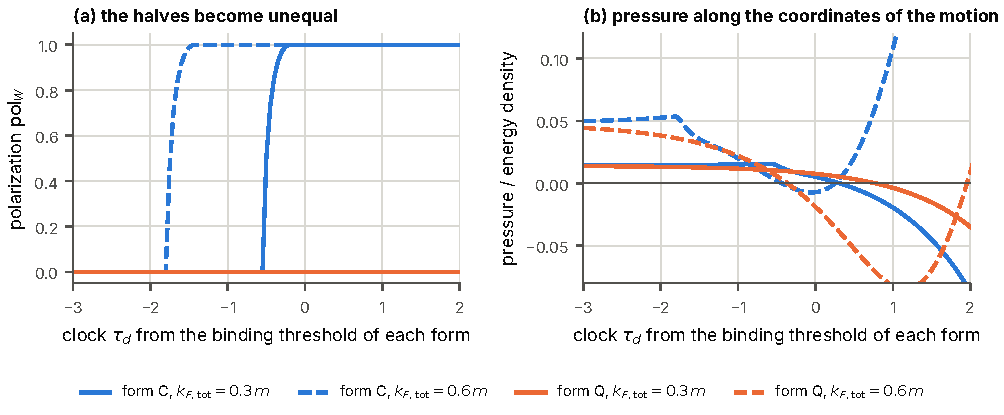
\includegraphics[width=0.86\textwidth]{fig_forms_gas}
\caption{\label{fig:ksgas}Matter of a fixed total density while the couplings grow ($D=4$, set A; the
clock of each form is counted from its own binding threshold). (a) The polarization: in form C the
two halves become unequal at a definite clock reading and one half empties soon after; in form Q
they stay equal. (b) The pressure along the coordinates of the motion, divided by the energy
density. Solid lines: $k_{F,\mathrm{tot}}=0.3\,m$; dashed lines: $0.6\,m$.}
\end{figure*}

\subsection{Form Q for other ratios of the couplings}
\label{sec:ksformq}

Matter of form Q with equal halves is matter of one kind of particle with eight internal states,
whose two couplings are the Hartree-Fock couplings, $\GS=\GS^{\mathrm{HF}}$ and
$\GV=\GV^{\mathrm{HF}}$; it is also the matter of the $7{+}1$ spacetime whose fields do not depend on
the deflating coordinates. For it the equations of Sec.~\ref{sec:ksmethod} hold with
$\GS(x4)=\GS^{\mathrm{ref}}e^{\td}$ and $\GV(x4)=\GV^{\mathrm{ref}}e^{\td}$, and
Table~\ref{tab:ksthrq} gives the smallest scalar attraction that binds it for three ratios of the two
couplings (the ratio 0.2025 is that of set B). The thresholds were computed twice, by the program
and by the independent script, and agree to $10^{-9}$.

\begin{table}
\caption{\label{tab:ksthrq}Form Q with equal halves (matter of one kind with eight internal states):
the smallest scalar attraction at which uniform matter is self-bound, for $D=4$ and $D=3$ and three
ratios of the vector repulsion to the scalar attraction, with the Fermi momentum of the bound state
at the threshold (units $m=1$). Last column: the critical coupling of the vacuum for a cutoff equal
to $m$ (Sec.~\ref{sec:sea}).}
\begin{ruledtabular}
\begin{tabular}{ccccc}
$D$ & $\GV/|\GS|$ & $|\GS|\,m^{D-1}$ & $\kF/m$ & $|G_c|\,m^{D-1}$ \\
\hline
4 & 0 & 62.0767 & 0.8879 & 29.6088 \\
4 & 0.1000 & 85.6504 & 0.7707 & 29.6088 \\
4 & 0.2025 & 119.5723 & 0.6792 & 29.6088 \\
3 & 0 & 8.0671 & 0.7932 & 4.9348 \\
3 & 0.1000 & 9.8364 & 0.7092 & 4.9348 \\
3 & 0.2025 & 12.2272 & 0.6351 & 4.9348 \\
\end{tabular}
\end{ruledtabular}
\end{table}

\section{Pairing and the gap along the clock}
\label{sec:gap}

\subsection{The pair channels}

A pair of fermions is created by an operator $\psi^{T}X\psi$ with a $16\times16$ matrix $X$; the
choice of $X$ is the \emph{channel} of the pair. For each channel one computes the \emph{exchange amplitudes} $F_S$ and $F_P$ of the radial mode and of the
phase mode: the matrix elements of the exchange of one boson between two fermions of opposite
momenta in the internal state of the channel. The radial mode attracts in every
channel, and the phase mode attracts in the four \emph{vector pairs along the extra axes},
\begin{equation}
\psi^{T}\Cm\gamma^{a}\psi,\qquad a\in\{0,5,6,7\},
\label{eq:pairs}
\end{equation}
and repels in their partners that are built with two Dirac matrices. Here
$\Cm=\gamma^{0}\gamma^{1}\gamma^{2}\gamma^{3}$
is the matrix that turns each Dirac matrix into minus its transpose (Sec.~\ref{sec:dirac}), and the index $a$ labels the
four extra axes. The pair along the hidden axis, $a=0$, has spin 0 in ordinary spacetime; it is the
\emph{hidden-axis singlet} of hypothesis H1.

The amplitudes are computed from the Dirac matrices of the frame, which the deflation does not
change, and each is proportional to the square of the coupling. For fields that do not depend on
$x5,x6,x7$ the amplitude of a channel at the time $x4$ is therefore
\begin{equation}
\begin{aligned}
F_{S,P}(x4)={}&\gVS(x4)^{2}\\
&\times\big(F_{S,P}\text{ of the flat spacetime at }\gVS=1\big).
\end{aligned}
\label{eq:amplitudes}
\end{equation}
The antisymmetric matrices $X$ fall into classes under the symmetries of the theory, with 15
representative channels. The program computes the amplitudes of these 15 channels from the
matrices of the deflating spacetime, at three momenta and 13 scattering angles; the numbers agree
with those computed with the matrices of flat spacetime to every digit,
and the amplitudes of the hidden-axis channel reproduce the closed forms of Eq.~(\ref{eq:Fclosed}) to $1.1\times10^{-15}$. The
conclusion about the channels therefore holds at every moment
(Fig.~\ref{fig:kernels}): the most attractive channel is the vector pair along an extra axis.

\begin{figure*}
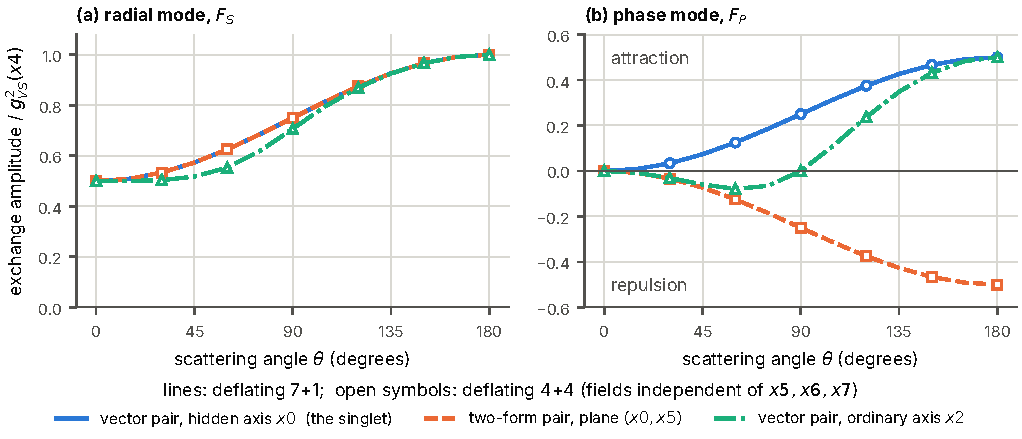
\includegraphics[width=0.84\textwidth]{fig_kernels}
\caption{\label{fig:kernels}Exchange amplitudes in three pair channels, divided by the square of the
coupling of the moment, against the scattering angle, for momenta of the magnitude $m$ in the plane
of $x1$ and $x2$. Lines: deflating $7{+}1$ spacetime; open symbols: deflating $4{+}4$ spacetime. (a) The
radial mode attracts in all three channels. (b) The phase mode attracts in the vector pair along the
hidden axis and repels in its partner built with two Dirac matrices. The amplitudes are those of flat
spacetime: the deflation changes their overall strength and nothing else.}
\end{figure*}

\subsection{The gap grows much faster than the coupling}

In matter of a given density the attraction opens a gap $\Delta_F$ at the Fermi momentum $\kF$: the
energy that it costs to break a pair. The gap equation [Eq.~(\ref{eq:gapeq}) below, where it is
written out with all its terms], which generalizes that
of Bardeen, Cooper and Schrieffer \cite{BCS1957}, holds at each moment with the couplings of that
moment. Its solution as a function of the clock is the \emph{adiabatic history} of the paired state:
the state that matter would have if it were always in equilibrium. (Section~\ref{sec:quench}
examines when it can be.) The strength of the pairing is measured by the dimensionless number
$\lambda=N(0)\,W(\kF,\kF)$, the density of states at the Fermi surface times the kernel of the gap
equation there; in the vector channel it is the sum $\lambda_S+\lambda_P$ of the contributions of the
two modes. Since the kernel is proportional to $\gVS^{2}$,
\begin{equation}
\lambda\ \propto\ e^{\td}.
\end{equation}

The program solves the gap equation at 34 moments for each of four sets of the mass $m_s$ and the
Fermi momentum (Table~\ref{tab:gap}, Fig.~\ref{fig:gap}). There are three results.

\begin{table*}
\caption{\label{tab:gap}The gap along the deflation clock for two of the four sets computed. $\gVS$
and $\lambda$: coupling and pairing strength of the moment. $\EF$: Fermi kinetic energy. $T_c$:
critical temperature. Rate of growth: $d\ln\Delta_F/d\td$; the last column, its product with
$\lambda$, is given where the gap is between $10^{-6}$ and $0.02$ of $\EF$.}
\begin{ruledtabular}
\begin{tabular}{cccccccc}
$m_s/m$, $\kF/m$ & $\td$ & $\gVS$ & $\lambda$ & $\Delta_F/\EF$ & $T_c/\Delta_F$ & rate of growth & $\lambda\,\times$ rate \\
\hline
0.10, 0.50 & $-0.63$ & 0.730 & 0.062 & $1.17\times10^{-7}$ & 0.567 & --- & --- \\
0.10, 0.50 & $-0.13$ & 0.939 & 0.102 & $7.40\times10^{-5}$ & 0.567 & 9.88 & 1.01 \\
0.10, 0.50 & 0.38 & 1.208 & 0.169 & $3.70\times10^{-3}$ & 0.567 & 6.01 & 1.01 \\
0.10, 0.50 & 0.88 & 1.554 & 0.279 & 0.0407 & 0.565 & 3.74 & --- \\
0.10, 0.50 & 1.39 & 2.000 & 0.463 & 0.189 & 0.555 & 2.50 & --- \\
0.10, 0.50 & 1.89 & 2.573 & 0.766 & 0.563 & 0.528 & 1.96 & --- \\
0.10, 0.50 & 2.39 & 3.311 & 1.268 & 1.49 & 0.480 & 1.96 & --- \\
1.0, 0.50 & 0.88 & 1.554 & 0.056 & $1.02\times10^{-7}$ & 0.567 & --- & --- \\
1.0, 0.50 & 1.13 & 1.763 & 0.072 & $5.62\times10^{-6}$ & 0.567 & 14.02 & 1.01 \\
1.0, 0.50 & 1.39 & 2.000 & 0.092 & $1.27\times10^{-4}$ & 0.567 & 10.93 & 1.01 \\
1.0, 0.50 & 1.64 & 2.269 & 0.119 & $1.45\times10^{-3}$ & 0.567 & 8.54 & 1.02 \\
1.0, 0.50 & 1.89 & 2.573 & 0.153 & $9.77\times10^{-3}$ & 0.567 & 6.71 & 1.03 \\
1.0, 0.50 & 2.14 & 2.919 & 0.197 & 0.0440 & 0.566 & 5.33 & --- \\
1.0, 0.50 & 2.39 & 3.311 & 0.253 & 0.148 & 0.563 & 4.38 & --- \\
\end{tabular}
\end{ruledtabular}
\end{table*}

\emph{The order of the channels does not change.} At every moment the gap of the vector channel is
at least as large as the gap that the radial mode alone would give, and that at least as large as
the gap of the channel in which the phase mode repels. The gap never decreases.

\emph{The critical temperature follows the gap.} Wherever the gap is below 5 per cent of the Fermi
kinetic energy $\EF$, the critical temperature is $T_c=0.567\,\Delta_F$, the ratio of weak coupling,
to within 0.002.

\emph{The law of growth.} In weak coupling the gap is proportional to $e^{-1/\lambda}$. With
$\lambda\propto e^{\td}$,
\begin{equation}
\frac{d\ln\Delta_F}{d\td}=\frac{1}{\lambda}.
\label{eq:growth}
\end{equation}
In the computed histories the product $\lambda\,d\ln\Delta_F/d\td$ lies between 1.00 and 1.03
wherever the gap is between $10^{-6}$ and $0.02$ of $\EF$.

Equation (\ref{eq:growth}) is the central quantitative statement about the superfluid on a deflating
spacetime. While the coupling grows by one e-folding, the gap of a weakly paired state with
$\lambda=0.1$ grows by ten e-foldings, a factor of twenty thousand. A paired state that is
unobservably weak at one time is strong a few e-foldings of the volume later.

\begin{figure*}
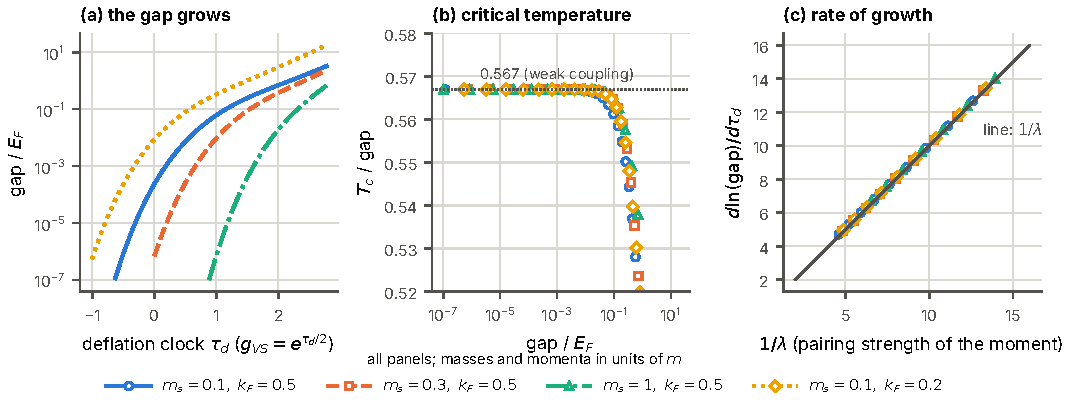
\includegraphics[width=\textwidth]{fig_gap_history}
\caption{\label{fig:gap}The gap along the deflation clock, for four sets of the mass of the radial
mode and of the Fermi momentum (in units of $m$). (a) The gap of the vector channel in units of the
Fermi kinetic energy. (b) The ratio of the critical temperature to the gap. (c) The rate of growth of
the gap against $1/\lambda$; the line is Eq.~(\ref{eq:growth}).}
\end{figure*}

\section{Pairing with the self-interaction}
\label{sec:gapcontact}

Section~\ref{sec:gap} treated the pairing by the exchange of the Vorton-Scalar alone. This section
adds the self-interaction of the fermion field. It writes out the amplitudes and the gap equation in
full, shows that the exchange of the Vorton-Scalar is itself a self-interaction of finite range,
gives the condition under which the gap equation has a solution that does not depend on the upper
limit of its momentum integral, and gives the gap along the deflation clock when both interactions
act. On the $4{+}4$ spacetime the contact couplings of form C enter the pair along the hidden axis
with the sign opposite to that of form Q, and the two forms select different pairs.

\subsection{Amplitudes of the four contact channels}

Two particles of the mass $\mst$ with the momenta $\vec p$ and $-\vec p$ in ordinary space scatter
into $\vec p'$ and $-\vec p'$. Let $E=(\mstq+p^{2})^{1/2}$ and $E'$ likewise, and let
$\hh(\vec p)=\sum_j\alpha^{j}p_j+\beta\,\mst$ be the Hamiltonian matrix of one particle, so that
$\tfrac12(1+\hh/E)$ projects on its states of positive energy. The pair along the hidden axis has
the wave function
\begin{equation}
\Phi(\vec p)=\tfrac12\Big(1+\frac{\hh(\vec p)}{E}\Big)\,X^{*}\,\tfrac12\Big(1+\frac{\hh(-\vec p)}{E}\Big)^{T},\qquad X=\Cm\gamma^{0},
\end{equation}
a $16\times16$ matrix. A vertex $\psi^\dagger\,\mathrm{Adj}\,\Theta^{K}\psi$ acting on both particles,
with the adjoint matrix $\mathrm{Adj}$ of the model, gives the amplitude
$\mathrm{Tr}[\Phi(\vec p')^\dagger\,\mathrm{Adj}\,\Theta^{K}\,\Phi(\vec p)\,(\mathrm{Adj}\,\Theta^{K})^{T}]$
divided by the norms of the two wave functions. Summed over the lists $K$ of one rank with the signs
$\sgnK$, this defines the amplitude of the rank $r$. In form Q ($\mathrm{Adj}=\beta$, matrices
$\ThQ^{K}$, signs $\sgnQ$), as on the $7{+}1$ spacetime, the result for the four independent channels of
Sec.~\ref{sec:four} is
\begin{equation}
\begin{aligned}
F_0&=\frac{EE'+\mstq-\vec p\cdot\vec p'}{2EE'},\\
F_1&=\frac{3EE'-2\mstq-\vec p\cdot\vec p'}{EE'},\\
F_7&=\frac{3EE'+2\mstq-\vec p\cdot\vec p'}{EE'},\\
F_8&=-\frac{EE'-\mstq-\vec p\cdot\vec p'}{2EE'} .
\end{aligned}
\label{eq:Fclosed}
\end{equation}
$F_0$ is the amplitude $F_S$ of the exchange of the radial mode of the Vorton-Scalar, which couples
to the scalar density, and $F_8=-F_P$ is minus the amplitude of the exchange of its phase mode,
which couples to the pseudoscalar density. At rest $(F_0,F_1,F_7,F_8)=(1,1,5,0)$, the pair coupling
(\ref{eq:Gpair}). The closed forms were verified against the direct evaluation with the 256 matrices
at random momenta, by the program to $1.8\times10^{-15}$ and by the independent script with
projectors built from numerical eigenvectors; the $7{+}1$ spacetime gives the same four
functions. They
hold for momenta in ordinary space; a momentum along the hidden axis itself changes them, because
the pair operator points along that axis.

\emph{The sign of the contact couplings in the two forms.} The same evaluation for the pairs along
$x5,x6,x7$, $\psi^{T}\Cm\gamma^{t}\psi$, and for both forms gives one rule. In form Q the amplitudes of
all four vector pairs along the extra axes are the functions (\ref{eq:Fclosed}). In form C
($\mathrm{Adj}=\Cm$) the amplitudes of the pairs along $x5,x6,x7$ are the same functions, and those of
the pair along the hidden axis are \emph{minus} these functions, at all momenta (direct evaluation
at random momenta, to $2.2\times10^{-15}$). This is Sec.~\ref{sec:pairs} at general momenta: the pair
along the hidden axis consists of one particle of each half of the field, the pairs along $x5,x6,x7$
of two particles of the same half. The contact amplitudes therefore enter the pairing potential with
a sign
\begin{equation}
\sct=\begin{cases}-1&\text{form C, pair along the hidden axis},\\+1&\text{form C, pairs along }x5,x6,x7,\\+1&\text{form Q, all four pairs}.\end{cases}
\label{eq:sct}
\end{equation}

The relations (\ref{eq:reduction}) between the nine invariants hold for the amplitudes at rest, and at
general momenta for the part of each amplitude that is even under $\vec p'\to-\vec p'$, which is the
sum of the direct and of the exchange scattering of two identical particles; they do not hold for
the odd part, which does not contribute to a contact interaction in a pair state without orbital
angular momentum. For a strictly local interaction the four couplings (\ref{eq:geff}) therefore
suffice. When the interaction is given a range, as below, the model is \emph{defined} by giving that
range to the four channels.

\subsection{The pairing potential and the gap equation}

The pairing potential of the contact interaction in each of these four pair channels is
\begin{equation}
V_{\mathrm{ct}}(\vec p',\vec p)=\sct\,\big(\geff0F_0+\geff1F_1+\geff7F_7+\geff8F_8\big)\,\frac{\mct^{2}}{q^{2}+\mct^{2}},
\label{eq:Vct}
\end{equation}
attractive where it is negative, with $q=|\vec p'-\vec p|$ and the sign (\ref{eq:sct}). A contact interaction in a gap equation
needs a regularization at large momentum transfer. The last factor gives each coupling the range
$1/\mct$ of an exchanged particle of the mass $\mct$, the \emph{range parameter}; it is the form that
the exchange of the Vorton-Scalar itself has:
\begin{equation}
V_{\mathrm{VS}}(\vec p',\vec p)=-\gVS^{2}\Big[\frac{F_S}{q^{2}+m_s^{2}}+\frac{F_P}{q^{2}+\mth^{2}}\Big],
\label{eq:VVS}
\end{equation}
with the mass $m_s$ of the radial mode and the mass $\mth$ of the phase mode, which vanishes when the
chiral symmetry is exact; it is the same in all four pair channels and in both forms, because the
Yukawa coupling contains the adjoint $\bar\psi$, in which the two halves of the field enter alike.
Comparing Eqs.~(\ref{eq:Vct}) and (\ref{eq:VVS}): \emph{the exchange of the
Vorton-Scalar is a self-interaction of finite range} of form Q, with the momentum-dependent couplings
\begin{equation}
\geff0(q)=-\frac{\gVS^{2}}{q^{2}+m_s^{2}},\qquad\geff8(q)=+\frac{\gVS^{2}}{q^{2}+\mth^{2}} .
\label{eq:gq_exchange}
\end{equation}
At momenta far below $m_s$ the radial mode acts as the scalar contact coupling
$g_0=-\gVS^{2}/m_s^{2}$ of form Q. In the phase with unbroken symmetry the two masses are equal and
$\geff0(q)+\geff8(q)=0$, the condition (\ref{eq:chiralcond}) of chiral invariance in form Q.
In the $4{+}4$ model of this paper the contact terms are of form C and the exchange is not: in the
pair along the hidden axis the two enter with opposite relative sign, and in the pairs along
$x5,x6,x7$ with the same. The program confirms
that the scalar contact coupling $-\gVS^{2}/m_s^{2}$ with $\mct=m_s$ reproduces the kernel of the
exchange of the radial mode to $3\times10^{-16}$.

The gap function $\Delta(k)$ of the paired state obeys, at the temperature $T$,
\begin{equation}
\begin{aligned}
\Delta(k)&=\frac{1}{4\pi^{2}}\int_0^{\kmax}dk'\,k'^{2}\,W(k,k')\,\frac{\Delta(k')}{E_{k'}}\tanh\frac{E_{k'}}{2T},\\
W(k,k')&=\frac12\int_{-1}^{1}d\cos\theta\,\big[-V_{\mathrm{VS}}-V_{\mathrm{ct}}\big],
\end{aligned}
\label{eq:gapeq}
\end{equation}
with $\xi_k=(k^{2}+m^{2})^{1/2}-\mu$, the quasi-particle energy $E_k=(\xi_k^{2}+\Delta(k)^{2})^{1/2}$,
the chemical potential $\mu=(\kF^{2}+m^{2})^{1/2}$, and the angle $\theta$ between $\vec p$ and
$\vec p'$ ($k=|\vec p|$, $k'=|\vec p'|$); $\Delta_F=\Delta(\kF)$; $\kmax$ is the upper limit of the
momentum integral, which the next subsection examines. It is the condition that the CJT
effective action be stationary with respect to the pair part of the propagator, in the truncation
of Sec.~\ref{sec:cjt}, and equally the form that the Kohn-Sham equations take with a pairing field.
The angular integral is elementary, because each amplitude is linear in $\cos\theta$.

\subsection{The upper limit of the momentum integral: an ultraviolet criterion}
\label{sec:uv}

At momenta far above all masses every term of the pairing potential has the form of a coupling
times a function of $\cos\theta$ divided by $q^{2}$, with $F_0,F_S,F_P\to\tfrac12(1-\cos\theta)$,
$F_8\to-\tfrac12(1-\cos\theta)$ and $F_1,F_7\to3-\cos\theta$. The kernel is then homogeneous,
$W(k,k')\to w_\infty(k'/k)/k^{2}$ with a function $w_\infty$ of the ratio of the two momenta, and
above the gap Eq.~(\ref{eq:gapeq}) at zero temperature reads
$\Delta(k)=\tfrac1{4\pi^{2}}\int_0^\infty dt\,t\,w_\infty(t)\,\Delta(tk)$. A power
$\Delta(k)\propto k^{-s_\Delta}$ solves it if the exponent $s_\Delta$ obeys
\begin{equation}
\int_0^\infty dt\;t^{1-s_\Delta}\,w_\infty(t)=4\pi^{2} .
\label{eq:uvroot}
\end{equation}
Because $W(k,k')$ is symmetric in its arguments, $w_\infty(1/t)=t^{2}\,w_\infty(t)$; the left-hand
side of Eq.~(\ref{eq:uvroot}) is therefore unchanged when $s_\Delta$ is replaced by $2-s_\Delta$, and
it is smallest at $s_\Delta=1$. Its value there is the \emph{ultraviolet strength} of the kernel,
\begin{equation}
\Uuv=\int_0^\infty dt\;w_\infty(t).
\label{eq:Uuvdef}
\end{equation}
If $\Uuv<4\pi^{2}$, Eq.~(\ref{eq:uvroot}) has two real roots, $s_\Delta>1$ and $2-s_\Delta<1$; the gap
function falls as $k^{-s_\Delta}$ with the larger root, and the gap equation has a solution that
does not depend on $\kmax$, which is approached as $\kmax^{-2(s_\Delta-1)}$, slowly when $\Uuv$ is
close to $4\pi^{2}$. If $\Uuv>4\pi^{2}$ the roots are complex, no such solution exists, and with an
upper limit the gap grows in proportion to $\kmax$: the pair collapses to short distances. This is
the fall to the center of relativistic particles in an attractive Coulomb potential whose strength
exceeds a critical value; the exchange of a boson of the mass $m_s$ gives a Yukawa potential, which
is a Coulomb potential at distances below $1/m_s$.

The integrals over $t$ and over the angle are elementary. With
$\int_0^\infty dt/(1+t^{2}-2t\cos\theta)=(\pi-\theta)/\sin\theta$ the two functions of the angle
give
\begin{equation}
\begin{aligned}
u_S&\equiv\int_0^\infty\!dt\,\frac12\int_{-1}^{1}\!d\cos\theta\,\frac{\tfrac12(1-\cos\theta)}{1+t^{2}-2t\cos\theta}=\frac{\pi^{2}}{8}-\frac12,\\
u_V&\equiv\int_0^\infty\!dt\,\frac12\int_{-1}^{1}\!d\cos\theta\,\frac{3-\cos\theta}{1+t^{2}-2t\cos\theta}=\frac{3\pi^{2}}{4}-1,
\end{aligned}
\label{eq:uSuV}
\end{equation}
that is $u_S=0.7337$ and $u_V=6.4022$, and therefore
\begin{equation}
\begin{aligned}
\Uuv={}&2\,u_S\,\gVS^{2}-\sct\,\mct^{2}\Big[\big(\geff0-\geff8\big)\,u_S\\
&+\big(\geff1+\geff7\big)\,u_V\Big]
\end{aligned}
\label{eq:Uuv}
\end{equation}
when both modes of the Vorton-Scalar are exchanged (half the first term for the radial mode alone).
The formula was verified against the numerical integral of the kernel by the program and by the
independent script. \emph{The exchange of the two modes alone reaches $\Uuv=4\pi^{2}$ at
$\gVS^{2}=4\pi^{2}/(2u_S)=26.90$}, the clock reading
$\td=3.29$ of the histories of Sec.~\ref{sec:gap}, beyond their last reading
2.77. A scalar contact attraction with $\sct=+1$ brings the criterion nearer, a
vector repulsion moves it away (Table~\ref{tab:uv}); with $\sct=-1$ it is the other way round, and
the vector contact coupling $+0.3\,\gVS^{2}/m^{2}$ in the hidden-axis pair of form C reaches the
criterion at $\gVS^{2}=11.65$, the clock reading $2.46$, from which
on no gap is given.

\begin{table*}
\caption{\label{tab:uv}The ultraviolet strength $\Uuv$ of the pairing kernel per unit $\gVS^{2}$, the
value of $\gVS^{2}$ at which it reaches $4\pi^{2}$, and the clock reading of that moment
($\gVS=e^{\td/2}$), for the exchange of the two modes of the Vorton-Scalar alone and with contact
couplings ($\mct=m$), for the two signs (\ref{eq:sct}). A dash: the criterion is never reached.}
\begin{ruledtabular}
\begin{tabular}{>{\raggedright\arraybackslash}p{0.3\textwidth}cccccc}
interaction & $\sct=+1$: $\Uuv/\gVS^{2}$ & critical $\gVS^{2}$ & $\td$ & $\sct=-1$: $\Uuv/\gVS^{2}$ & critical $\gVS^{2}$ & $\td$ \\
\hline
exchange of the Vorton-Scalar alone & 1.467 & 26.90 & 3.29 & 1.467 & 26.90 & 3.29 \\
with $g_0^{\mathrm{eff}}=-g_{\mathrm{VS}}^2/m^2$ & 2.201 & 17.94 & 2.89 & 0.734 & 53.81 & 3.99 \\
with $g_0^{\mathrm{eff}}=-g_{\mathrm{VS}}^2/m^2$, $g_1^{\mathrm{eff}}=+0.1\,g_{\mathrm{VS}}^2/m^2$ & 1.561 & 25.29 & 3.23 & 1.374 & 28.73 & 3.36 \\
with $g_1^{\mathrm{eff}}=+0.3\,g_{\mathrm{VS}}^2/m^2$ & $-0.453$ & --- & --- & 3.388 & 11.65 & 2.46 \\
with $g_7^{\mathrm{eff}}=-0.1\,g_{\mathrm{VS}}^2/m^2$ & 2.108 & 18.73 & 2.93 & 0.827 & 47.73 & 3.87 \\
contact couplings alone ($g_0^{\mathrm{eff}}=-g_{\mathrm{VS}}^2/m^2$, $g_1^{\mathrm{eff}}=+0.1\,g_{\mathrm{VS}}^2/m^2$) & 0.093 & 422.32 & 6.05 & $-0.093$ & --- & --- \\
\end{tabular}
\end{ruledtabular}
\end{table*}

The criterion was tested numerically: the gap was computed with the upper limits $\kmax=60$,
$2\times10^{3}$, $2\times10^{4}$ and $2\times10^{5}$, in units of the larger of $m$ and $\kF$, for
192 kernels (four sets of $m_s$ and $\kF$, four clock readings, seven combinations of
couplings, and both signs of the contact part). Below the criterion the gap converges
(Table~\ref{tab:uvclasses}); above it (8 kernels)
it grows by a factor between 11.49 and 14.56 from $\kmax=2\times10^{4}$
to $2\times10^{5}$, so that its value is not a property of the model. \emph{All gaps of this paper are
computed with $\kmax=2\times10^{4}$, and none is given above the criterion.} A limit of 60, with
which gaps of this model were computed before, gives gaps of the exchange alone that are too small
by up to 1.08 per cent at the strongest coupling of the histories, and gaps with
contact couplings that are too small by up to the percentages of the last column of the table.

\begin{table}
\caption{\label{tab:uvclasses}Convergence of the gap with the upper limit $\kmax$ of the momentum
integral, by classes of the ultraviolet strength (the kernels of both signs of the contact part that
lie below the criterion and have a gap above $10^{-4}$ of the Fermi kinetic energy): the largest
relative change of the gap from
$\kmax=2\times10^{4}$ to $2\times10^{5}$, and the largest error of the limit $\kmax=60$.}
\begin{ruledtabular}
\begin{tabular}{lccc}
$\Uuv/4\pi^{2}$ & kernels & change & error of 60 (per cent) \\
\hline
$U_{\mathrm{uv}}/4\pi^2<0.5$ & 118 & $2.5\times10^{-6}$ & 0.75 \\
$0.5$ to $0.7$ & 28 & $6.4\times10^{-5}$ & 2.37 \\
$0.7$ to $0.9$ & 8 & $3.3\times10^{-3}$ & 12.59 \\
\end{tabular}
\end{ruledtabular}
\end{table}

\subsection{The gap along the clock with contact couplings}

All couplings of the four-dimensional description grow as $e^{\td}$ (Sec.~\ref{sec:clock}), so that
the ratio of a contact coupling to $\gVS^{2}$ is fixed. Table~\ref{tab:gapcontact} and
Fig.~\ref{fig:paircontact} give the gap, for the sign $\sct=+1$, for seven choices: the exchange alone; the exchange with a
scalar contact attraction $\geff0=-\gVS^{2}/m^{2}$; with a scalar attraction and a vector repulsion
one tenth as large, $\geff1=+0.1\,\gVS^{2}/m^{2}$; with a vector repulsion alone,
$\geff1=+0.3\,\gVS^{2}/m^{2}$; with an axial coupling $\geff7=-0.1\,\gVS^{2}/m^{2}$; the contact
couplings without the Vorton-Scalar; and the exchange alone with a phase mode of the mass
$\mth=0.3\,m$. The range parameter is $\mct=m$.

\begin{table*}
\caption{\label{tab:gapcontact}The gap at the Fermi surface in units of the Fermi kinetic energy,
with contact couplings that enter with the sign $\sct=+1$ (form Q, all four vector pairs along the
extra axes; form C, the pairs along $x5,x6,x7$), at the clock reading 2.04
[$\gVS=2.771$], for the Fermi
momentum $\kF=0.5\,m$ and three masses of the radial mode. Contact couplings in units of
$\gVS^{2}/m^{2}$; $\mct=m$.}
\begin{ruledtabular}
\begin{tabular}{lccc}
interaction & $m_s=0.1\,m$ & $m_s=0.3\,m$ & $m_s=m$ \\
\hline
exchange of the Vorton-Scalar alone & 0.7504 & 0.4118 & 0.0247 \\
with a scalar contact attraction, $g_0^{\mathrm{eff}}=-1$ & 1.2895 & 0.9035 & 0.2975 \\
with $g_0^{\mathrm{eff}}=-1$ and $g_1^{\mathrm{eff}}=+0.1$ & 1.1105 & 0.7407 & 0.1963 \\
with a vector contact repulsion, $g_1^{\mathrm{eff}}=+0.3$ & 0.5438 & 0.2370 & 0.0006 \\
with an axial-vector contact coupling, $g_7^{\mathrm{eff}}=-0.1$ & 1.0114 & 0.6459 & 0.1290 \\
contact couplings alone, $g_0^{\mathrm{eff}}=-1$, $g_1^{\mathrm{eff}}=+0.1$ & 0.0006 & 0.0006 & 0.0006 \\
exchange alone, phase mode of the mass $0.3\,m$ & 0.7341 & 0.3967 & 0.0197 \\
\end{tabular}
\end{ruledtabular}
\end{table*}

\begin{figure*}
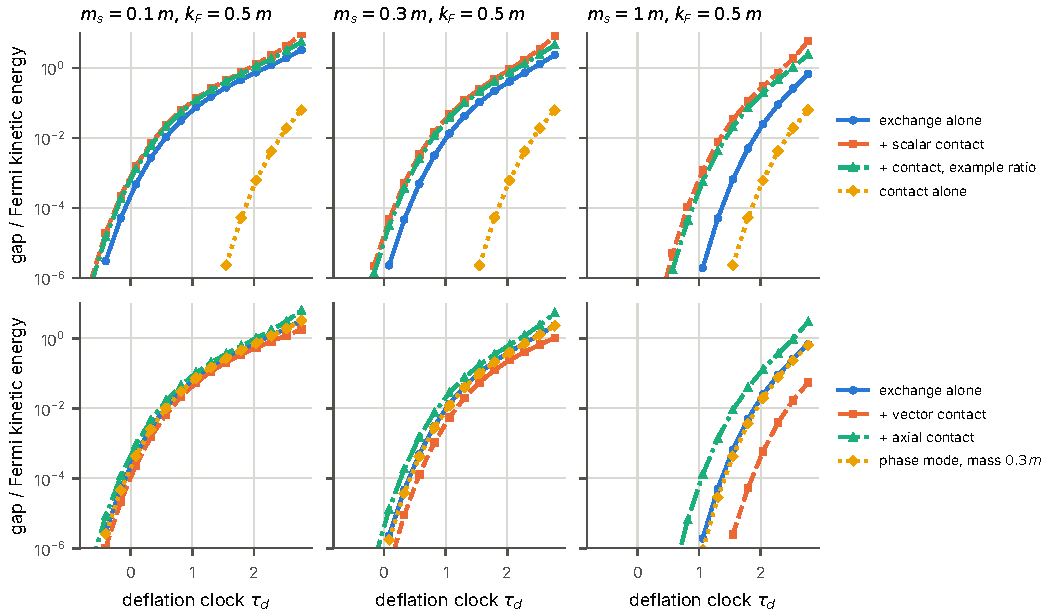
\includegraphics[width=\textwidth]{fig_pair_contact}
\caption{\label{fig:paircontact}The gap with contact couplings that enter with the sign $\sct=+1$
(form Q; form C in the pairs along $x5,x6,x7$) along the deflation clock, for the Fermi momentum $0.5\,m$ and three masses $m_s$ of the radial mode of the
Vorton-Scalar. Upper row: the exchange of the Vorton-Scalar alone; with a scalar contact attraction;
with a scalar attraction and a vector repulsion one tenth as large; the contact couplings alone.
Lower row: the exchange alone; with a vector contact repulsion; with an axial contact coupling; with
a phase mode of the mass $0.3\,m$. Couplings and range parameter as in
Table~\ref{tab:gapcontact}.}
\end{figure*}

Three statements summarize the result for $\sct=+1$; each was verified at every clock reading at
which the gap exceeds $10^{-6}$ of the Fermi kinetic energy.

\emph{A scalar contact attraction raises the gap}, strongly so where the exchange alone is weak: for
$m_s=m$ at the clock reading of Table~\ref{tab:gapcontact} by the factor 12.1.

\emph{A vector contact repulsion lowers it.} A vector coupling of three tenths of $\gVS^{2}/m^{2}$
removes most of the gap of a weakly paired state (Table~\ref{tab:gapcontact}, $m_s=m$) and reduces
the gap of a strongly paired one.

\emph{A mass of the phase mode lowers it}, because it weakens the attraction of that mode at small
momentum transfer.

Without contact couplings the program reproduces the gaps of Sec.~\ref{sec:gap} to $7\times10^{-16}$.
For small gaps the critical temperature remains $0.567$ times the gap. An independent solution of
Eq.~(\ref{eq:gapeq}) on another grid of momenta, by plain iteration, gives the gaps of
Table~\ref{tab:gapcontact} for the first three rows to $8.2\times10^{-7}$ (relative). The law of growth
(\ref{eq:growth}) holds with contact couplings as it does without, because every part of the kernel
grows as $e^{\td}$.

\subsection{The pair along the hidden axis in form C}
\label{sec:gapformc}

In the definition of the model, form C, the contact couplings enter the pair along the hidden axis
with $\sct=-1$. Table~\ref{tab:gapsign} and Fig.~\ref{fig:gapsign} compare the two signs for the same
couplings. With $\sct=-1$ the couplings act in the opposite way: \emph{a scalar contact attraction
lowers the gap} (for $m_s=m$ it removes it at the clock reading of the table), an axial coupling
$\geff7<0$ lowers it, and \emph{a vector contact repulsion raises it}; the contact couplings of the
signs of set B alone give no gap in this pair at any clock reading. The gap with $\sct=-1$ and the
vector coupling agrees with an independent solution of the gap equation to $7.8\times10^{-5}$.

\begin{table*}
\caption{\label{tab:gapsign}The gap at the Fermi surface in units of the Fermi kinetic energy at the
clock reading 2.04, for $\kF=0.5\,m$ and two masses of the radial mode, for the two
signs with which the contact couplings enter the pairing potential: $\sct=+1$ (form Q; form C in the
pairs along $x5,x6,x7$) and $\sct=-1$ (form C in the pair along the hidden axis). Last two columns:
the ultraviolet strength of the kernel for $m_s=m$. Contact couplings in units of $\gVS^{2}/m^{2}$;
$\mct=m$.}
\begin{ruledtabular}
\begin{tabular}{>{\raggedright\arraybackslash}p{0.3\textwidth}cccccc}
interaction & $m_s=0.3\,m$, $\sct=+1$ & $-1$ & $m_s=m$, $\sct=+1$ & $-1$ & $\Uuv/4\pi^{2}$, $\sct=+1$ & $-1$ \\
\hline
exchange of the Vorton-Scalar alone & 0.4118 & 0.4118 & 0.0247 & 0.0247 & 0.285 & 0.285 \\
with $g_0^{\mathrm{eff}}=-g_{\mathrm{VS}}^2/m^2$ & 0.9035 & 0.1481 & 0.2975 & 0.0000 & 0.428 & 0.143 \\
with $g_0^{\mathrm{eff}}=-g_{\mathrm{VS}}^2/m^2$, $g_1^{\mathrm{eff}}=+0.1\,g_{\mathrm{VS}}^2/m^2$ & 0.7407 & 0.1875 & 0.1963 & 0.0000 & 0.304 & 0.267 \\
with $g_1^{\mathrm{eff}}=+0.3\,g_{\mathrm{VS}}^2/m^2$ & 0.2370 & 0.8481 & 0.0006 & 0.2285 & $-0.088$ & 0.659 \\
with $g_7^{\mathrm{eff}}=-0.1\,g_{\mathrm{VS}}^2/m^2$ & 0.6459 & 0.2509 & 0.1290 & 0.0007 & 0.410 & 0.161 \\
contact couplings alone ($g_0^{\mathrm{eff}}=-g_{\mathrm{VS}}^2/m^2$, $g_1^{\mathrm{eff}}=+0.1\,g_{\mathrm{VS}}^2/m^2$) & 0.0006 & 0.0000 & 0.0006 & 0.0000 & 0.018 & $-0.018$ \\
\end{tabular}
\end{ruledtabular}
\end{table*}

\begin{figure*}
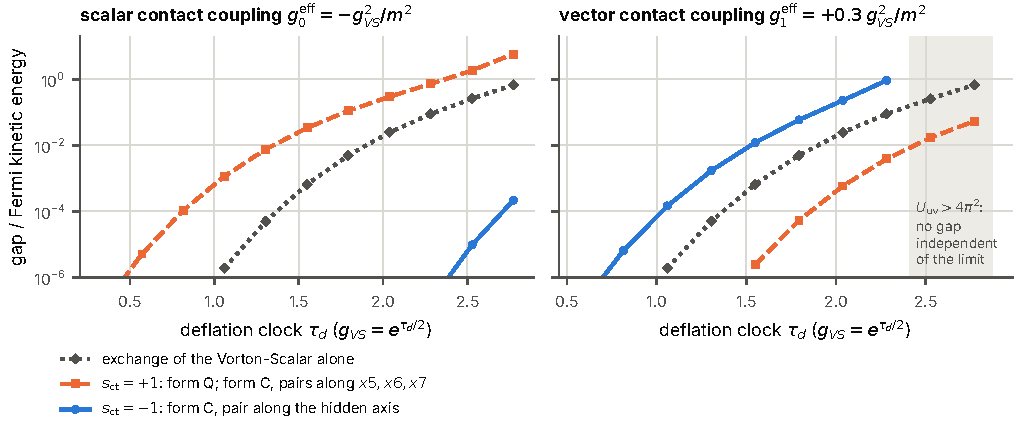
\includegraphics[width=0.86\textwidth]{fig_forms_gap}
\caption{\label{fig:gapsign}The gap at the Fermi surface, in units of the Fermi kinetic energy, along
the deflation clock, for $m_s=m$ and $\kF=0.5\,m$. Left: with the scalar contact coupling
$\geff0=-\gVS^{2}/m^{2}$; right: with the vector contact coupling $\geff1=+0.3\,\gVS^{2}/m^{2}$. Dotted
line: the exchange of the Vorton-Scalar alone. Dashed line (squares): the contact coupling with the
sign $\sct=+1$ (form Q; form C in the pairs along $x5,x6,x7$). Solid line (circles): with the sign
$\sct=-1$ (form C in the pair along the hidden axis). In the shaded band the kernel with $\sct=-1$
exceeds the ultraviolet criterion of Sec.~\ref{sec:uv}, and no gap is given.}
\end{figure*}

\emph{In form C the self-interaction removes the degeneracy of the pair along the hidden axis with
the pairs along $x5,x6,x7$, and so selects the direction of the order parameter}
(Table~\ref{tab:gapwins}). With an attractive scalar coupling the pairs along the additional
time-like axes have the larger gap, not the pair along the hidden axis; with a repulsive vector
coupling alone the pair along the hidden axis has the larger gap. In form Q, as on the $7{+}1$
spacetime, the four pairs have the same gap, and the direction is free (Sec.~\ref{sec:order}).

\begin{table}
\caption{\label{tab:gapwins}Form C: the number of clock readings, among those at which both gaps are
defined, at which the pairs along $x5,x6,x7$ ($\sct=+1$) or the pair along the hidden axis
($\sct=-1$) have the larger gap (four sets of $m_s$ and $\kF$).}
\begin{ruledtabular}
\begin{tabular}{p{0.52\columnwidth}cc}
interaction & $x5,x6,x7$ & hidden axis \\
\hline
with $g_0^{\mathrm{eff}}=-g_{\mathrm{VS}}^2/m^2$ & 53 & 0 \\
with $g_0^{\mathrm{eff}}=-g_{\mathrm{VS}}^2/m^2$, $g_1^{\mathrm{eff}}=+0.1\,g_{\mathrm{VS}}^2/m^2$ & 53 & 0 \\
with $g_1^{\mathrm{eff}}=+0.3\,g_{\mathrm{VS}}^2/m^2$ & 0 & 43 \\
with $g_7^{\mathrm{eff}}=-0.1\,g_{\mathrm{VS}}^2/m^2$ & 51 & 0 \\
\end{tabular}
\end{ruledtabular}
\end{table}

\section{The bound pair and the order of events}
\label{sec:pair}

\subsection{The moment of binding}

Two fermions in the Yukawa potential (\ref{eq:yukawa}) form a bound state if and only if the number
$\DVS$ of Eq.~(\ref{eq:DC}) exceeds a critical value, $D_c=1.67981$. On a deflating spacetime
$\DVS\propto e^{\td}$, so that the pair becomes bound at a definite time. Measure the clock from that
moment:
\begin{equation}
\tpair=\ln\frac{\DVS}{D_c}=\gsum\,\big(x4-x4_{\mathrm{binding}}\big).
\label{eq:tpair}
\end{equation}
Table~\ref{tab:dimer} and Fig.~\ref{fig:binding} show the scattering length $a_{\mathrm{sc}}$ of two
fermions and the binding energy $E_b$ of the pair as the clock passes the binding. The linearized
gap equation in vacuum, whose kernel is relativistic, gives nearly the same critical value: 1.7347,
1.6902 and 1.6810 for $m_s/m=0.3$, $0.1$ and $0.03$ (Table~\ref{tab:xthreshold}).

\begin{table}
\caption{\label{tab:dimer}Two fermions as the clock passes the moment of binding: the scattering
length in units of $1/m_s$, the number of bound states, and the binding energy in units of
$m_s^{2}/m$.}
\begin{ruledtabular}
\begin{tabular}{ccccc}
$\tpair$ & $\DVS$ & $a_{\mathrm{sc}}\,m_s$ & bound states & $E_b\,m/m_s^{2}$ \\
\hline
$-0.105$ & 1.5118 & $-12.50$ & 0 & 0 \\
$-0.095$ & 1.5279 & $-13.93$ & 0 & 0 \\
$-0.010$ & 1.6630 & $-134.0$ & 0 & 0 \\
0.010 & 1.6966 & 135.9 & 1 & $5.50\times10^{-5}$ \\
0.486 & 2.7314 & 2.698 & 1 & 0.232 \\
0.994 & 4.5409 & $-0.1288$ & 1 & 1.82 \\
\end{tabular}
\end{ruledtabular}
\end{table}

\emph{The scattering length.} Just before the binding the scattering length is large and negative,
just after it large and positive: $-134.0/m_s$ at $0.99\,D_c$ and $+135.9/m_s$ at $1.01\,D_c$. At the
moment of binding it is infinite: the two fermions are at a scattering resonance. \emph{Every pair
of fermions of the model passes through this resonance once, at the same time.}
Section~\ref{sec:cosmo} examines what that means if the fermions are the dark matter.

\emph{The binding energy.} Just after the binding the binding energy starts quadratically,
\begin{equation}
E_b\ \propto\ \big(e^{\tpair}-1\big)^{2}\,\frac{m_s^{2}}{m},
\label{eq:Eb}
\end{equation}
with the fitted exponent 2.01 between 2 and 8 per cent above $D_c$. Because $E_b$ vanishes at the
threshold, the time $1/E_b$ that the pair needs to adjust is infinite there. However slow the
deflation is, the pair cannot follow it adiabatically at first.

\emph{The same threshold from the gap equation.} In vacuum the linearized gap equation is the
equation of a bound state of two fermions, with a relativistic kernel. It reaches the eigenvalue 1 at
$\DVS=1.7347$, $1.6902$ and $1.6810$ for $m_s/m=0.3$, $0.1$ and $0.03$, approaching the value
$D_c$ of the Schr\"odinger equation as the radial mode becomes light and the binding
non-relativistic.

\begin{figure*}
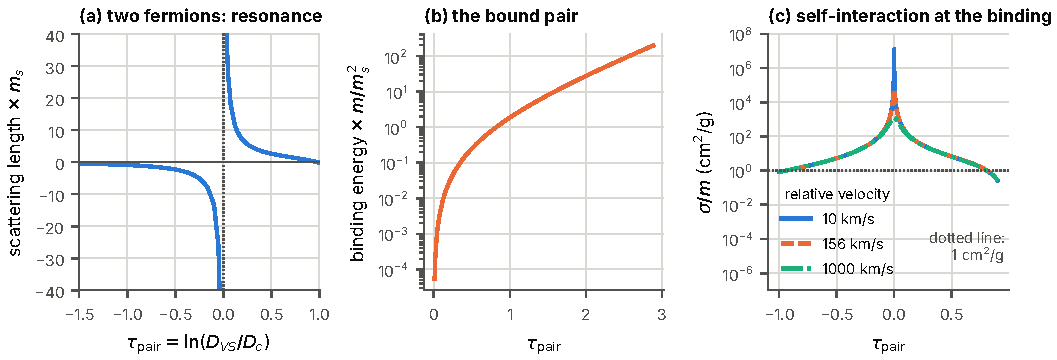
\includegraphics[width=\textwidth]{fig_binding}
\caption{\label{fig:binding}The bound pair along the clock. (a) Scattering length of two fermions in
units of $1/m_s$ against $\tpair$: the resonance at the moment of binding. (b) Binding energy of the
pair. (c) Cross-section per mass of two fermions at three relative velocities while the clock passes
the binding, for the example particle of Sec.~\ref{sec:dm}.}
\end{figure*}

\subsection{The order of events}

The other thresholds of the model are thresholds in the number $C$ of Eq.~(\ref{eq:DC}),
which grows at the same rate as $\DVS$. Because $C/\DVS=4\pi m/m_s$ is fixed, the order in which the
events happen depends on the ratio $m_s/m$ alone. Table~\ref{tab:events} gives the clock reading
$\tpair$ of each event; a negative number means that the event precedes the binding of the pair. The
events other than the binding are derived in Sec.~\ref{sec:cjt}.

\begin{table*}
\caption{\label{tab:events}The order of events along the deflation: the clock reading $\tpair$ of
each event, relative to the moment at which two fermions form a bound pair, for six ratios of the
mass $m_s$ of the radial mode to the fermion mass $m$.}
\begin{ruledtabular}
\begin{tabular}{p{0.42\textwidth}lcccccc}
event & threshold & $0.1$ & $0.3$ & $1$ & $3$ & $10$ & $30$ \\
\hline
the one-loop potential of the Vorton-Scalar falls below its vacuum value at the field $10\,v_{\mathrm{VS}}$ & $C=1.5477$ & $-4.92$ & $-3.82$ & $-2.61$ & $-1.51$ & $-0.31$ & 0.79 \\
matter is self-bound (Fermi sea only) & $C=3.7011$ & $-4.04$ & $-2.94$ & $-1.74$ & $-0.64$ & 0.56 & 1.66 \\
the one-loop potential falls below its vacuum value at the field $3\,v_{\mathrm{VS}}$ & $C=4.2694$ & $-3.90$ & $-2.80$ & $-1.60$ & $-0.50$ & 0.70 & 1.80 \\
matter is self-bound (with the negative-energy states) & $C=5.9218$ & $-3.57$ & $-2.48$ & $-1.27$ & $-0.17$ & 1.03 & 2.13 \\
matter of Fermi momentum $0.5\,m$ becomes abnormal (massless fermions) & $C=12.9713$ & $-2.79$ & $-1.69$ & $-0.49$ & 0.61 & 1.82 & 2.91 \\
\textbf{two fermions form a bound pair} & $D_{\mathrm{VS}}=1.6798$ & 0.00 & 0.00 & 0.00 & 0.00 & 0.00 & 0.00 \\
pair condensate in the vacuum (ladder equation, cutoff $100\,m$) & $\alpha_{\mathrm{VS}}=2.13$ to $2.93$ & 2.54 & 1.44 & 0.25 & $-0.82$ & $-1.93$ & $-2.84$ \\
\end{tabular}
\end{ruledtabular}
\end{table*}

For a \emph{light radial mode}, $m_s/m\le3$ in the table, the pair becomes bound only \emph{after}
the one-loop potential of the Vorton-Scalar has fallen below its vacuum value at a field of three
times the vacuum value: the deflation endangers the vacuum of the model before it binds the pair. The
condition for the opposite order is $4\pi D_c\,m/m_s<4.27$, that is, $m_s/m>4.9$. For a \emph{heavy
radial mode}, $m_s/m=10$ or $30$, the pair becomes bound first, and matter becomes self-bound and
loses its fermion mass later. Nothing in the model decides between the two orders; the table states
what follows from each.

\section{Can the paired state follow the deflation?}
\label{sec:quench}

\subsection{The question, and the parameter that decides it}

Section~\ref{sec:gap} gave the gap that the paired state would have in equilibrium at each moment.
But a state can change at most at the rate of its own energy scale, which for a paired state is the
gap. By Eq.~(\ref{eq:growth}) the equilibrium gap, written $\Deq$ in this section, changes at the
rate $\gsum/\lambda$. The paired state can follow only if that rate is small compared with the gap
itself:
\begin{equation}
\Xid=\frac{\gsum}{\lambda\,\Deq}\ \ll\ 1 .
\label{eq:Xi}
\end{equation}
Early in the deflation the gap is exponentially small, and the condition fails however small the
rate is. A system that is carried through a change faster than it can respond falls out of
equilibrium, as in the formation of defects at a phase transition \cite{Kibble1976,Zurek1985}. The
question is what the paired state does then, and when it catches up.

\subsection{The model}

The question is answered with the standard reduced model of a superfluid, whose dynamics without
collisions is known in detail \cite{BarankovLevitovSpivak2004}. Pairs of states of opposite momenta,
with the single-particle energy $\xi_k$ measured from the Fermi energy, fill a shell
$-\Esh<\xi_k<\Esh$ with a constant density of states, and all attract one another with the
dimensionless strength $\lambda$. In the mean-field approximation each pair of states is described by
its pair correlation $\kappa$, a complex number, and its occupation $n_k$; the order parameter is
$\Delta=\lambda\int\kappa\,d\xi_k$. The equations of motion are
\begin{align}
\frac{d\kappa}{dx4}&=-i\,\big[2\,\xi_k\,\kappa-\Delta\,(1-2n_k)\big],\nonumber\\
\frac{dn_k}{dx4}&=2\,\mathrm{Im}\big(\Delta^{*}\kappa\big).
\label{eq:bloch}
\end{align}
They conserve $|2\kappa|^{2}+(1-2n_k)^{2}=1$ for every pair of states. In equilibrium
$\kappa=\Delta/2E_k$ and $n_k=\tfrac12(1-\xi_k/E_k)$ with the quasi-particle energy
$E_k=(\xi_k^{2}+\Delta^{2})^{1/2}$, and the gap equation gives
\begin{equation}
\Deq(\lambda)=\frac{\Esh}{\sinh(1/\lambda)}\ \approx\ 2\,\Esh\,e^{-1/\lambda}\quad(\lambda\ll1).
\end{equation}
The model keeps what matters for the question, a gap that depends exponentially on a coupling that
grows exponentially, and omits the dependence of the gap on the momentum; $\Esh$ stands for the
range of energies over which the attraction acts. The program starts the model in equilibrium at
$\lambda=0.15$, lets the coupling grow as $\lambda=0.15\,e^{\td}$ up to $\lambda=0.5$, and integrates
Eqs.~(\ref{eq:bloch}) for 2000 energies. Doubling the number of energies and halving the step
changes no digit of the results quoted. Besides $|\Delta|$ the program records the density $\nex$ of
\emph{broken pairs}: the number of pairs of states, per unit of $\Esh$ times the density of states,
that are not in the ground state that belongs to the order parameter of the moment. In equilibrium
it is zero.

\subsection{Results}

\begin{table*}
\caption{\label{tab:quench}The paired state while the pairing strength grows from 0.15 to 0.5, for
seven rates of deflation: the parameter $\Xid$ at the start; the smallest ratio of the order
parameter to the equilibrium gap of the moment; the clock reading at which the order parameter has
returned to within 10 per cent of the equilibrium gap, and $\Xid$ at that moment; the ratio at the
end; and the density of broken pairs at the end.}
\begin{ruledtabular}
\begin{tabular}{ccccccc}
$\gsum/\Esh$ & $\Xid$ at the start & smallest $|\Delta|/\Deq$ & $\td$ of the catch-up & $\Xid$ there & final $|\Delta|/\Deq$ & $\nex$ at the end \\
\hline
$1\times10^{-4}$ & 0.262 & 0.958 & 0.020 & 0.23 & 1.0000 & $6.0\times10^{-6}$ \\
$3\times10^{-4}$ & 0.786 & 0.890 & 0.069 & 0.47 & 0.9998 & $5.1\times10^{-5}$ \\
$1\times10^{-3}$ & 2.62 & 0.737 & 0.234 & 0.52 & 0.9980 & $4.4\times10^{-4}$ \\
$3\times10^{-3}$ & 7.86 & 0.539 & 0.454 & 0.44 & 0.9886 & $2.4\times10^{-3}$ \\
0.01 & 26.2 & 0.328 & 0.780 & 0.32 & 0.9347 & 0.012 \\
0.03 & 78.6 & 0.189 & 1.172 & 0.24 & 0.8076 & 0.041 \\
0.1 & 262 & 0.098 & --- & --- & 0.1189 & 0.022 \\
\end{tabular}
\end{ruledtabular}
\end{table*}

Table~\ref{tab:quench} and Fig.~\ref{fig:quench} show three results.

\emph{The faster the deflation, the further the order parameter falls behind.} For a rate of
$10^{-4}\,\Esh$ the order parameter drops to 0.958 of the equilibrium gap of the moment before it
recovers; for $10^{-1}\,\Esh$ it drops to 0.098.

\emph{The state catches up when $\Xid$ has fallen to a value between 0.23 and 0.52.} In six of the
seven runs the order parameter returns to within 10 per cent of the equilibrium gap at such a value.
In the fastest run it has not caught up when the coupling reaches 0.5. This confirms the estimate
(\ref{eq:Xi}) and fixes the number that ``small'' means.

\emph{The lag leaves broken pairs behind.} Their density at the end grows with the rate, from
$6.0\times10^{-6}$ to $4.1\times10^{-2}$ in the six slower runs. They are excitations of the
superfluid that the deflation itself has made; in a system without dissipation they remain.

Because $\Deq$ grows as $e^{-1/\lambda}$ while $\lambda$ grows only as $e^{\td}$, the parameter
$\Xid$ falls steeply with time. For any rate there is a moment at which $\Xid$ passes through the
window of the second result. Before it the paired state is out of equilibrium, with an order
parameter below the equilibrium value; after it the adiabatic history of Sec.~\ref{sec:gap}
applies. The slower the deflation, the earlier that moment and the smaller the gap at which it
happens: it is the moment at which the equilibrium gap has grown to between two and four times
$\gsum/\lambda$.

\begin{figure*}
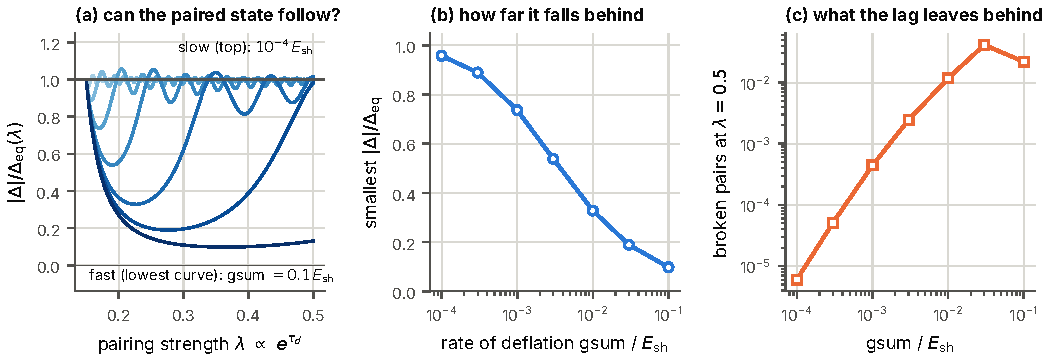
\includegraphics[width=\textwidth]{fig_quench}
\caption{\label{fig:quench}The paired state while the coupling grows. (a) The order parameter
divided by the equilibrium gap of the moment, against the pairing strength, for seven rates of
deflation. (b) The smallest value of that ratio against the rate. (c) The density of broken pairs at
the end of the run against the rate.}
\end{figure*}

\section{The effective action along the clock}
\label{sec:cjt}

\subsection{The method, and why it carries over}

The results on the paired state, on matter, on temperature and on the
vacuum follow from the effective action for composite operators of Cornwall, Jackiw and Tomboulis (CJT)
\cite{CJT1974}: a functional of the expectation value $\phi$ of the Vorton-Scalar and of the full
propagators, whose two-particle-irreducible part is truncated at two loops. Its stationarity
conditions are the equation for the fermion mass in matter and the gap equation. On the deflating
spacetime, and for fields that do not depend on the extra coordinates, nothing in this construction
changes, for two reasons established above. The weighted fermion field obeys the flat equations, so
that its propagator is the flat one. And the interaction between the fermions is, at each moment,
the exchange of the two modes of the scalar with the coupling of that moment and with the unshifted
range (Sec.~\ref{sec:scalarmodes}).

The one new term, the shift $-\gsum^{2}/4$ of the squares of the boson masses in
Eq.~(\ref{eq:couplings}), is smaller than every other scale of the calculation by the square of the
ratio of the rate of deflation to a particle mass. For the largest rate that observation allows
(Sec.~\ref{sec:cosmo}) and a mass of 1~keV that ratio is below $10^{-36}$. The term is neglected in
this section; this is the only approximation made here beyond the truncation itself. The test
of the truncation on a solvable model in zero dimensions, which does not involve the spacetime, was
executed again: the two-loop truncation has a solution for every coupling from 0.01 to 30 and stays
within 10.7 per cent of the exact propagator.

Every result of this section is a statement about a \emph{sequence of equilibrium states}. Whether a
system can follow the sequence was examined, for the paired state, in Sec.~\ref{sec:quench}.

\subsection{The paired state}

The CJT potential $V[\Delta]$ of the paired state is the effective action per unit volume, measured
from the unpaired state, as a functional of the gap function $\Delta(k)$. The program evaluates it at
13 moments, for two choices of the mass $m_s$ at the Fermi momentum $\kF=0.5\,m$, in the vector
channel (Table~\ref{tab:cjt}, Fig.~\ref{fig:cjt}).

\begin{table*}
\caption{\label{tab:cjt}The paired state along the clock from the CJT potential, for $\kF=0.5\,m$.
$\lambda$: pairing strength. $V$: the potential at the solution, the condensation energy. Ratio: $V$
divided by its weak-coupling value $-\nu N(0)\Delta_F^{2}/4$, with $\nu=8$ internal states and the
density of states $N(0)$. Curvature: the smallest eigenvalue of the matrix of second derivatives of
the potential. Size: the coherence length of the pair in units of $1/\kF$.}
\begin{ruledtabular}
\begin{tabular}{cccccccccc}
$m_s/m$, $\kF/m$ & $\td$ & $\gVS$ & $\lambda$ & $\Delta_F/m$ & $V/m^{4}$ & ratio & curvature & $T_c/\Delta_F$ & size $\times\kF$ \\
\hline
0.30, 0.50 & 0.00 & 1.80 & 0.216 & $2.81\times10^{-3}$ & $-4.46\times10^{-7}$ & 1.000 & 0.21 & 0.567 & 25.4 \\
0.30, 0.50 & 0.21 & 2.00 & 0.266 & $6.89\times10^{-3}$ & $-2.68\times10^{-6}$ & 0.998 & 0.26 & 0.566 & 10.3 \\
0.30, 0.50 & 0.40 & 2.20 & 0.322 & 0.0135 & $-1.03\times10^{-5}$ & 0.992 & 0.30 & 0.564 & 5.3 \\
0.30, 0.50 & 0.58 & 2.40 & 0.383 & 0.0230 & $-2.93\times10^{-5}$ & 0.981 & 0.34 & 0.559 & 3.1 \\
0.30, 0.50 & 0.74 & 2.60 & 0.450 & 0.0354 & $-6.82\times10^{-5}$ & 0.961 & 0.37 & 0.552 & 2.0 \\
0.30, 0.50 & 0.88 & 2.80 & 0.522 & 0.0511 & $-1.38\times10^{-4}$ & 0.932 & 0.38 & 0.542 & 1.4 \\
0.30, 0.50 & 1.02 & 3.00 & 0.599 & 0.0707 & $-2.53\times10^{-4}$ & 0.895 & 0.38 & 0.530 & 1.0 \\
1.0, 0.50 & 0.00 & 2.40 & 0.133 & $4.25\times10^{-4}$ & $-1.02\times10^{-8}$ & 1.000 & 0.13 & 0.567 & 167.5 \\
1.0, 0.50 & 0.16 & 2.60 & 0.156 & $1.32\times10^{-3}$ & $-9.90\times10^{-8}$ & 1.000 & 0.15 & 0.567 & 53.8 \\
1.0, 0.50 & 0.31 & 2.80 & 0.181 & $3.28\times10^{-3}$ & $-6.09\times10^{-7}$ & 0.999 & 0.17 & 0.567 & 21.7 \\
1.0, 0.50 & 0.45 & 3.00 & 0.208 & $6.90\times10^{-3}$ & $-2.69\times10^{-6}$ & 0.998 & 0.19 & 0.566 & 10.3 \\
1.0, 0.50 & 0.58 & 3.20 & 0.237 & 0.0128 & $-9.29\times10^{-6}$ & 0.994 & 0.21 & 0.564 & 5.5 \\
1.0, 0.50 & 0.70 & 3.40 & 0.267 & 0.0219 & $-2.67\times10^{-5}$ & 0.987 & 0.23 & 0.561 & 3.3 \\
\end{tabular}
\end{ruledtabular}
\end{table*}

\emph{The solution of the gap equation is a minimum at every moment.} Newton's method applied to the
potential converges to the gap function that the iteration of the gap equation finds, to
$7.7\times10^{-12}$, and the smallest eigenvalue of the second variation is positive throughout. The
temperature at which the second variation at $\Delta=0$ loses its positivity equals the temperature
at which the linearized gap equation has the eigenvalue 1, to $2.6\times10^{-12}$: two routes to the
critical temperature agree.

\emph{The condensation energy deepens.} It is within 15 per cent of the weak-coupling value wherever
the gap is below $0.1\,\EF$, and in weak coupling its logarithmic slope along the clock is twice that
of the gap, by Eq.~(\ref{eq:growth}):
\begin{equation}
\frac{d\ln|V|}{d\td}=\frac{2}{\lambda}.
\end{equation}

\emph{The pairs shrink.} The coherence length of the first set falls from 25 to 1.0 in units of
$1/\kF$. At its last five moments the gap exceeds $0.1\,\EF$, and at the last the pair is as small
as the distance between the particles. \emph{The deflation carries the paired state from overlapping
pairs toward bound pairs.} On flat spacetime this crossover \cite{NozieresSchmittRink1985,Leggett1975}
is reached by choosing a larger coupling; here it is reached by waiting.

\emph{The universal ratios hold while the coupling is weak.} While the critical temperature rises by
a factor of sixteen, from $6.3\times10^{-3}$ to $0.10$ of the Fermi energy, the ratio of the gap at
zero temperature to the critical temperature stays within 0.019 of the weak-coupling value 1.7639,
and the relative jump of the heat capacity at $T_c$ within 0.048 of 1.4261. The coefficients of the
Ginzburg-Landau energy agree with their weak-coupling formulas to 1.2 per cent while $T_c$ is below
$0.05\,\EF$ and differ by up to 9.8 per cent at $T_c=0.10\,\EF$. The coherence length of the
Ginzburg-Landau energy, $0.1333\,v_F/T_c$ in weak coupling with the Fermi velocity $v_F$, shrinks
from 80 to 5.1 in units of $1/m$: the cores of the vortices of the superfluid shrink as the
deflation proceeds. Tables~\ref{tab:xthermo} and \ref{tab:xgl} of Appendix~\ref{app:tables} give
the numbers at the three moments computed.

\begin{figure*}
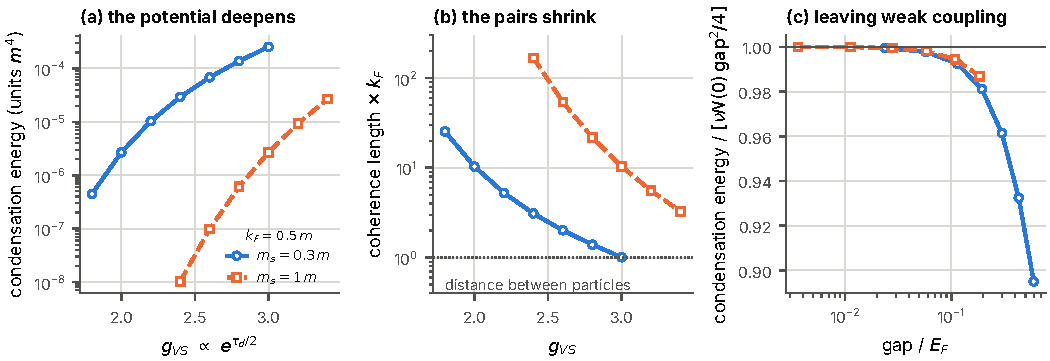
\includegraphics[width=\textwidth]{fig_cjt_history}
\caption{\label{fig:cjt}The paired state along the clock, from the CJT potential, for the two sets of
Table~\ref{tab:cjt}. (a) The condensation energy against the coupling of the moment. (b) The
coherence length of the pair in units of $1/\kF$. (c) The condensation energy divided by its
weak-coupling value, against the gap in units of the Fermi kinetic energy: the departure from weak
coupling.}
\end{figure*}

\subsection{Matter}

\emph{Matter of fixed density loses its fermion mass.} In matter the expectation value of the
Vorton-Scalar is reduced by the scalar density of the fermions, and with it the fermion mass in the
matter, $m^{*}$. The reduction depends on the density and on the
single number $C$, and above a critical value of $C$ the mass vanishes: the matter is then in
the \emph{abnormal} state of Lee and Wick \cite{LeeWick1974}, a gas of massless fermions in a region
without expectation value of the scalar. On the deflating spacetime $C\propto e^{\td}$ grows at
fixed density. The critical values are $C=151.892$, $12.971$, $2.556$ and $0.617$ for the Fermi
momenta $\kF=0.2$, $0.5$, $1$ and $2$ in units of $m$; they exceed the estimate
$\pi^{2}m^{2}/4\kF^{2}$, which holds for dense matter, by the factors 2.46, 1.31, 1.04 and 1.00. \emph{Every
piece of matter becomes abnormal at a definite moment, the denser the earlier.}

\emph{Self-bound matter.} Matter is self-bound, that is, its energy per particle at some density
lies below the mass of a free fermion, if $C>3\pi^{2}/8=3.7011$ without the filled negative-energy
states and if $C>3\pi^{2}/5=5.9218$ with them. Once the threshold is passed, the lowest energy per
particle falls monotonically along the clock (Table~\ref{tab:saturation}), from $-0.0192\,m$ at
$C=4$ to $-0.405\,m$ at $C=29.6$. At every one of these moments the matter of lowest energy is in the
abnormal state. The exchange energies of the two modes, which the mean field omits, are 0.44 and
0.51 per cent of the mean-field energy at the first moment and 0.90 and 1.22 per cent at the last
(for $m_s/m=0.3$):
the mean field remains a good approximation along the whole history. A gas of the fermions that is
dilute and unbound at early times thus has, at late times, a state of lower energy: drops of dense
abnormal matter, bound by up to 40 per cent of the rest mass at the last moment of the table.
Whether and how fast a gas reaches that state is a question of kinetics that is not answered here.

\begin{table}
\caption{\label{tab:saturation}Self-bound matter along the clock, in the mean-field approximation
without the negative-energy states, for $C=4\,e^{\td}$: the lowest energy per particle minus the
fermion mass, and the Fermi momentum at which it is reached.}
\begin{ruledtabular}
\begin{tabular}{cccc}
$\td$ & $C$ & $(E/N-m)/m$ & $\kF/m$ \\
\hline
0.00 & 4.00 & $-0.0192$ & 0.981 \\
0.25 & 5.14 & $-0.0787$ & 0.921 \\
0.50 & 6.59 & $-0.1345$ & 0.866 \\
0.75 & 8.47 & $-0.1869$ & 0.813 \\
1.00 & 10.87 & $-0.2362$ & 0.764 \\
1.25 & 13.96 & $-0.2825$ & 0.718 \\
1.50 & 17.93 & $-0.3259$ & 0.674 \\
1.75 & 23.02 & $-0.3668$ & 0.633 \\
2.00 & 29.56 & $-0.4051$ & 0.595 \\
\end{tabular}
\end{ruledtabular}
\end{table}

\subsection{Temperature}

At high temperature the expectation value of the Vorton-Scalar vanishes and the fermions are
massless. The temperature $T_{1/2}$ at which the expectation value has fallen to one half is of the
order of the four-dimensional vacuum value $\vVS=m/\gVS$, which falls as $e^{-\td/2}$ while the
masses stay fixed. In units of the constant fermion mass, $T_{1/2}$ falls monotonically as the
coupling grows, for each of the three ratios $m_s/m=0.3$, $1$ and $3$ examined; for $m_s/m=1$, from
$2.33\,m$ at $\gVS=0.3$ to $0.37\,m$ at $\gVS=4$ [Fig.~\ref{fig:matter}(d)]. \emph{Matter of a fixed
temperature melts at a definite moment of the deflation.} For $m_s/m=0.3$ no melting temperature
can be given from $C=32$ on: there the one-loop potential of the vacuum turns over so close to the
vacuum value that the Hartree potential ceases to exist before the expectation value has fallen, and
the program marks these moments as not defined (Table~\ref{tab:xthermal}).

\subsection{The vacuum}

The one-loop potential of the Vorton-Scalar in vacuum contains the negative contribution of the
fermion loop \cite{ColemanWeinberg1973}, which grows with the fourth power of the field and
eventually wins: beyond some field the potential lies below its value in the vacuum. The larger $C$,
the smaller that field: 24.7 times the vacuum value at $C=1$, and 1.77 times at $C=10$
[Fig.~\ref{fig:matter}(c), Table~\ref{tab:xvacuum}]. As the deflation proceeds, the barrier between the vacuum of the model
and the region where the one-loop potential is unbounded below moves in toward the vacuum.

The one-loop potential is not reliable at fields far from the vacuum value, and a potential that
falls at large field signals that the effective theory needs completion there, not that the vacuum
decays. What the result establishes is a trend: every statement of the model that rests on the
vacuum of the Vorton-Scalar becomes less secure with time. The order of this event relative to the
binding of the pair was given in Sec.~\ref{sec:pair}.

\emph{A pair condensate in the vacuum.} The ladder equation with a
momentum cutoff shows that the pair can condense without a medium only if $\aVS$ exceeds a critical value
$\alpha_c$ of order one \cite{Miransky1985}; with the cutoff $100\,m$ the critical values lie between
2.13 and 2.93 for the six mass ratios of Table~\ref{tab:events}. On the deflating spacetime $\aVS$
reaches such a value at a definite moment. But at that moment the coupling is strong, the exchange
of one boson is no longer a controlled approximation, and the vacuum of the model is no longer
protected. A pair condensate in the vacuum is not reached by the deflation within the range of
validity of the model.

\begin{figure*}
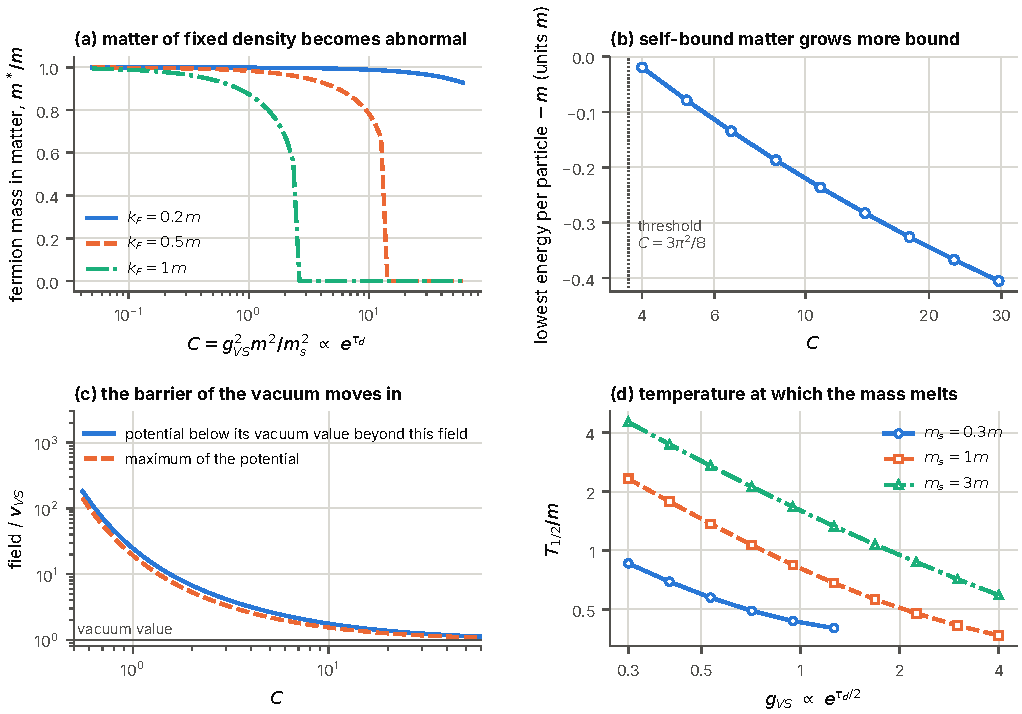
\includegraphics[width=0.92\textwidth]{fig_matter_history}
\caption{\label{fig:matter}Matter, vacuum and temperature along the clock. (a) The fermion mass in
matter of three fixed densities against $C\propto e^{\td}$: it drops to zero at the critical value.
(b) The lowest energy per particle of self-bound matter, minus $m$. (c) The field at which the
one-loop potential of the vacuum has its maximum, and the field beyond which it lies below the vacuum
value, in units of the vacuum value. (d) The temperature at which the fermions have lost half of
their mass, against the coupling, for three ratios $m_s/m$.}
\end{figure*}

\section{The effective potential with the self-interaction}
\label{sec:cjtcontact}

Section~\ref{sec:cjt} applied the effective action of Cornwall, Jackiw and Tomboulis to the model
in which the Vorton-Scalar alone provides mass and interaction. This section applies the same
method to the self-interaction of the fermion field: first without the Vorton-Scalar, where it must
reproduce the Kohn-Sham results of Sec.~\ref{sec:ks} and goes beyond them by counting the filled
states of negative energy; then with the bare Dirac mass, the self-interaction and the Vorton-Scalar
together.

\subsection{The effective potential of uniform matter}

The CJT effective action is a functional of the full propagator $S$ of the fermions,
\begin{equation}
\Gamma[S]=-i\,\mathrm{Tr}\ln S^{-1}-i\,\mathrm{Tr}\big(S_0^{-1}S-1\big)+\Gamma_2[S],
\label{eq:GammaCJT}
\end{equation}
where $S_0$ is the propagator of free particles of the mass $m$ and $\Gamma_2$ is the sum of the
vacuum diagrams that cannot be cut in two by cutting two lines, drawn with the full propagator. For
the contact interaction $\Lself$ the lowest order of $\Gamma_2$ consists of two diagrams, each with
two loops that meet at one vertex: the direct (Hartree) and the exchange (Fock) diagram. At this
order the stationarity condition $\delta\Gamma/\delta S=0$ says that the self-energy
$S_0^{-1}-S^{-1}$ does not depend on the momentum. For uniform matter at rest it is a combination of
the unit matrix and of $\beta$ (Sec.~\ref{sec:hf}): the full propagator is that of free particles of
a mass $\mst$ whose energies are shifted by a constant $V_0$. The effective action per unit volume
and time then becomes an ordinary function of the two numbers $\mst$ and $V_0$, the \emph{effective
potential}. At zero temperature and at the chemical potential $\mu$,
\begin{align}
\Omega_{\mathrm{CJT}}&(\mst,V_0;\mu)=-\frac{(\mst-m)^{2}}{2\,\GS}-\frac{V_0^{2}}{2\,\GV}\nonumber\\
&-\nu\!\int\!\frac{d^{D}k}{(2\pi)^{D}}\,\big(\mu-V_0-E^{*}\big)\,\theta\big(\mu-V_0-E^{*}\big),
\label{eq:OmegaCJT}
\end{align}
with $E^{*}=(k^{2}+\mstq)^{1/2}$, the step function $\theta$, and the scalar and vector coupling
$\GS$, $\GV$ of matter of one kind of particle with $\nu$ internal states (Sec.~\ref{sec:ksmethod}). The integral is the grand potential of free particles of the mass $\mst$ at
the chemical potential $\mu-V_0$; the two other terms remove the interaction energy that the
integral counts twice. The two stationarity conditions are
\begin{equation}
\begin{aligned}
\frac{\partial\Omega_{\mathrm{CJT}}}{\partial V_0}&=0:\quad V_0=\GV\,n,\\
\frac{\partial\Omega_{\mathrm{CJT}}}{\partial\mst}&=0:\quad\mst=m+\GS\,\nS ,
\end{aligned}
\label{eq:CJTstat}
\end{equation}
the two equations (\ref{eq:hKS}) of the Kohn-Sham method. At the stationary point
$-\Omega_{\mathrm{CJT}}$ is the pressure and $\Omega_{\mathrm{CJT}}+\mu\,n$ the energy density.
\emph{The Kohn-Sham method and the CJT effective potential at this order are two formulations of the
same approximation}: the first works at a fixed density and solves the gap equation, the second
works at a fixed chemical potential and searches the stationary point of a function.

The program evaluates the two with separate code (Gauss-Legendre integrals and a root search in the
one, Simpson integrals and a minimization in the other) for 30 states in $D=7$,
$4$ and $3$ dimensions (Table~\ref{tab:cjtks}). Mass, density, energy density and pressure agree to
$1.6\times10^{-12}$ (sum of the four relative deviations); the independent script repeats the
comparison with its own integrals and finds the same.

\begin{table}
\caption{\label{tab:cjtks}The Kohn-Sham method (KS) and the CJT effective potential compared, without
the filled states of negative energy (units $m=1$): the mass of the particles in matter by both
methods, and $-\Omega_{\mathrm{CJT}}$ at its stationary point divided by the Kohn-Sham pressure $p$,
for ten of the 30 states computed (the data files hold eleven digits).}
\begin{ruledtabular}
\begin{tabular}{ccccccc}
$D$ & $\GS$ & $\GV$ & $\kF$ & $\mst$ (KS) & $\mst$ (CJT) & $-\Omega_{\mathrm{CJT}}/p$ \\
\hline
7 & $-100000$ & $10000$ & 0.9 & 0.143888 & 0.143888 & 1.00000000 \\
7 & $-100000$ & $10000$ & 1.4 & 0.011510 & 0.011510 & 1.00000000 \\
7 & $-98750$ & $20000$ & 0.9 & 0.145495 & 0.145495 & 1.00000000 \\
7 & $-98750$ & $20000$ & 1.4 & 0.011654 & 0.011654 & 1.00000000 \\
4 & $-256.9512$ & $25.6951$ & 0.9 & 0.140053 & 0.140053 & 1.00000000 \\
4 & $-256.9512$ & $25.6951$ & 1.4 & 0.040348 & 0.040348 & 1.00000000 \\
3 & $-29.5093$ & $2.9509$ & 0.9 & 0.182319 & 0.182319 & 1.00000000 \\
3 & $-29.5093$ & $2.9509$ & 1.4 & 0.079333 & 0.079333 & 1.00000000 \\
3 & $-4$ & $0$ & 0.9 & 0.394848 & 0.394848 & 1.00000000 \\
3 & $-4$ & $0$ & 1.4 & 0.240321 & 0.240321 & 1.00000000 \\
\end{tabular}
\end{ruledtabular}
\end{table}

The effective potential says more than the gap equation in one respect. At a given chemical
potential the stationary point with the lowest $\Omega_{\mathrm{CJT}}$, that is, with the highest
pressure, is the state of equilibrium (the vector field $V_0$ is taken at its stationary value, a
maximum; the minimum is over $\mst$). Of the 23 states of the comparison with a
positive pressure, 20 are that minimum. In the others a denser state has the higher
pressure at the same chemical potential: the Kohn-Sham state of that density is metastable, a dilute
gas that can lower its energy by condensing into saturated matter.

\emph{The two halves of the field.} For the matter of Sec.~\ref{sec:ksreduced}, whose two halves have
different masses and energy shifts, the effective potential is a function of four numbers,
\begin{equation}
\begin{aligned}
\Omega_{\mathrm{CJT}}={}&\sum_\pm\Omega_{\mathrm{half}}\big(\mstpm,\mu-V_{0\pm}\big)\\
&-\frac{\big[\tfrac12(m^{*}_++m^{*}_-)-m\big]^{2}}{2\,\GStot}-\frac{\big[\tfrac12(m^{*}_+-m^{*}_-)\big]^{2}}{2\,\GSdif}\\
&-\frac{\big[\tfrac12(V_{0+}+V_{0-})\big]^{2}}{2\,\GVtot}-\frac{\big[\tfrac12(V_{0+}-V_{0-})\big]^{2}}{2\,\GVdif},
\end{aligned}
\label{eq:OmegaHalves}
\end{equation}
where $\Omega_{\mathrm{half}}(\mst,\mu)=-4\int d^{D}k\,(\mu-E^{*})\,\theta(\mu-E^{*})/(2\pi)^{D}$ is the
grand potential of free particles of one half, with four internal states. Its four stationarity
conditions are the equations (\ref{eq:hKShalves}) with the densities (\ref{eq:denshalves}). For
80 states of both forms (40 with equal halves,
17 with unequal halves, 23 with one half filled) the
stationary point, found by Newton's method from displaced start values, agrees with the Kohn-Sham
state in both masses, density, energy density and pressure to $4.9\times10^{-11}$: the two methods
are equivalent in both forms.

\subsection{The filled states of negative energy}
\label{sec:sea}

The Kohn-Sham calculation counts the particles of matter only. The term
$-i\,\mathrm{Tr}\ln S^{-1}$ of Eq.~(\ref{eq:GammaCJT}) also contains the filled states of negative
energy of the vacuum, whose energy depends on the mass of the particles. Because the contact
interaction is an effective interaction, their momenta are counted up to a cutoff $\Lambda$:
\begin{equation}
\begin{aligned}
\Omega_{\mathrm{CJT}}\to{}&\Omega_{\mathrm{CJT}}-\nu\!\int_{|\vec k|<\Lambda}\!\frac{d^{D}k}{(2\pi)^{D}}\\
&\times\Big[\sqrt{k^{2}+\mstq}-\sqrt{k^{2}+m^{2}}\Big].
\end{aligned}
\label{eq:sea}
\end{equation}
The filled states contribute the scalar density
$-\nu\int_{|\vec k|<\Lambda}d^{D}k\,(\mst/E^{*})/(2\pi)^{D}$ to the gap equation. The mass parameter
of the Lagrangian is then no longer the mass of a particle in vacuum and is called the \emph{bare
mass} $m_{\mathrm{bare}}$; the mass in vacuum, $m_{\mathrm{vac}}$, is the solution of
\begin{equation}
\begin{aligned}
m_{\mathrm{vac}}&=m_{\mathrm{bare}}+\GS\,\langle\bar\psi\psi\rangle_{\mathrm{vac}},\\
\langle\bar\psi\psi\rangle_{\mathrm{vac}}&=-\nu\!\int_{|\vec k|<\Lambda}\!\frac{d^{D}k}{(2\pi)^{D}}\,\frac{m_{\mathrm{vac}}}{\sqrt{k^{2}+m_{\mathrm{vac}}^{2}}} .
\end{aligned}
\label{eq:mvac}
\end{equation}
The scalar density of the vacuum is negative, so that an attraction ($\GS<0$) \emph{raises} the mass
above the bare mass.

\emph{A critical coupling.} For $m_{\mathrm{bare}}=0$ Eq.~(\ref{eq:mvac}) always has the solution
$m_{\mathrm{vac}}=0$. A second solution, of lower energy, exists if the attraction exceeds a
critical value, $\GS<G_c$. Expanding the integral for small $m_{\mathrm{vac}}$, with the area
$A_D=D\,V_D$ of the unit sphere,
\begin{equation}
\begin{aligned}
G_c&=-\frac{(2\pi)^{D}\,(D-1)}{\nu\,A_D\,\Lambda^{D-1}},\\
G_c\,\Lambda^{D-1}&=-90\pi^{4},\ -3\pi^{2},\ -\frac{\pi^{2}}{2}\quad\text{for }D=7,\ 4,\ 3 .
\end{aligned}
\label{eq:Gc}
\end{equation}
\emph{A field without a mass term acquires a mass by its own self-interaction when the scalar
attraction exceeds $G_c$.} This is the mechanism of Nambu and Jona-Lasinio \cite{NJL1961};
the minimization of the effective potential gives no mass two per cent below $G_c$ and a mass two
per cent above it in all three cases.

\emph{On the deflating spacetime the critical coupling is crossed at a definite moment.} In the
sector of fields that do not depend on $x5,x6,x7$ the coupling grows as $e^{\td}$ while the cutoff,
a momentum along the flat coordinates, does not change. A field that is massless at early times
therefore acquires a mass at the clock reading $\td=\ln[G_c/\GS(x4_{\mathrm{ref}})]$, and from then
on the mass grows [Fig.~\ref{fig:cjtsea}(a), Table~\ref{tab:cjtvac}]. With a small bare mass the
transition is smooth. The mass reaches the cutoff about half a unit of the clock after the critical
coupling is crossed; beyond that point the effective theory says nothing. (Table~\ref{tab:cjtvac}
and Fig.~\ref{fig:cjtsea} are for one kind of particle with eight internal states, that is, for form Q
of the $4{+}4$ model and for the $7{+}1$ model; the two halves of the field in form C follow below.)

\begin{table}
\caption{\label{tab:cjtvac}The mass of the fermions in vacuum, $m_{\mathrm{vac}}/\Lambda$, with the
filled states of negative energy, along the deflation clock counted from the moment at which
$\GS=G_c$, for a field without bare mass and for the bare mass $0.05\,\Lambda$.}
\begin{ruledtabular}
\begin{tabular}{cccccc}
$D$ & $m_{\mathrm{bare}}/\Lambda$ & $\td=-1$ & $\td=0$ & $\td=0.24$ & $\td=0.48$ \\
\hline
7 & 0 & 0 & 0 & 0.658 & 1.074 \\
7 & 0.05 & 0.079 & 0.436 & 0.774 & 1.154 \\
4 & 0 & 0 & 0 & 0.544 & 0.913 \\
4 & 0.05 & 0.079 & 0.383 & 0.664 & 0.995 \\
3 & 0 & 0 & 0 & 0.447 & 0.780 \\
3 & 0.05 & 0.078 & 0.335 & 0.573 & 0.866 \\
\end{tabular}
\end{ruledtabular}
\end{table}

\begin{figure*}
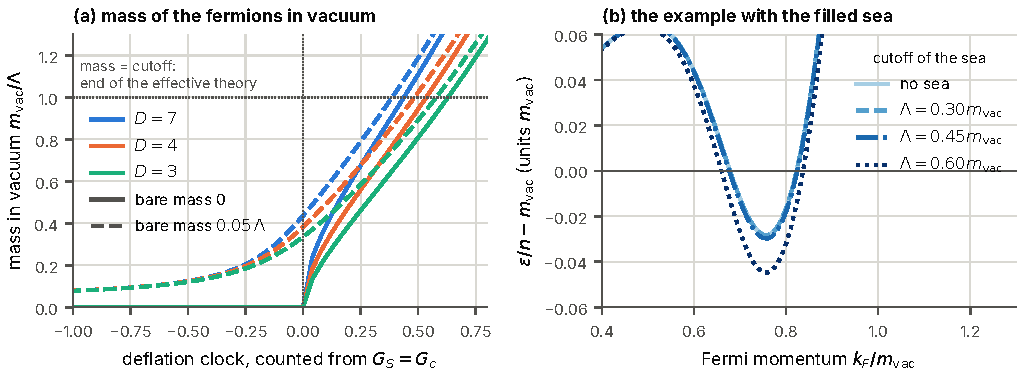
\includegraphics[width=0.86\textwidth]{fig_cjt_sea}
\caption{\label{fig:cjtsea}The filled states of negative energy. (a) The mass of the fermions in
vacuum, in units of the cutoff, along the deflation clock counted from the moment at which the
scalar attraction equals the critical coupling, for $D=7$, $4$ and $3$ dimensions, without bare mass
and with the bare mass $0.05\,\Lambda$. (b) Energy per particle of matter relative to the vacuum, for
an example on the $7{+}1$ spacetime ($D=7$,
$\GS=-10^{5}$, $\GV=+10^{4}$ in units of the mass in vacuum) without the filled states and with them
for three cutoffs; the bare mass is chosen so that the mass in vacuum is the same.}
\end{figure*}

\emph{The vacuum of the two halves.} For the two halves of the field the gap equations of the
vacuum are
\begin{equation}
\begin{aligned}
\tfrac12(m^{*}_++m^{*}_-)-m_{\mathrm{bare}}&=\GStot\,\big(n_{S+}^{\mathrm{vac}}+n_{S-}^{\mathrm{vac}}\big),\\
\tfrac12(m^{*}_+-m^{*}_-)&=\GSdif\,\big(n_{S+}^{\mathrm{vac}}-n_{S-}^{\mathrm{vac}}\big),\\
n_{S\pm}^{\mathrm{vac}}&=-4\!\int_{|\vec k|<\Lambda}\!\frac{d^{D}k}{(2\pi)^{D}}\,\frac{\mstpm}{E^{*}_\pm},
\end{aligned}
\label{eq:vachalves}
\end{equation}
with the scalar densities $n_{S\pm}^{\mathrm{vac}}$ of the filled states of the two halves; where they
have several solutions, the vacuum is the one of lowest energy density
\begin{equation}
\begin{aligned}
\Omega_{\mathrm{vac}}={}&-4\sum_\pm\!\int_{|\vec k|<\Lambda}\!\frac{d^{D}k}{(2\pi)^{D}}\Big[E^{*}_\pm-\sqrt{k^{2}+m_{\mathrm{bare}}^{2}}\Big]\\
&-\frac{\big[\tfrac12(m^{*}_++m^{*}_-)-m_{\mathrm{bare}}\big]^{2}}{2\,\GStot}-\frac{\big[\tfrac12(m^{*}_+-m^{*}_-)\big]^{2}}{2\,\GSdif} .
\end{aligned}
\end{equation}
For the sets A and B the more attractive of the two scalar couplings is $\GS^{\mathrm{HF}}$ in both
forms ($\GStot$ in form Q, $\GSdif$ in form C), so that the critical strength
$g_{\mathrm{crit}}=G_c\,g/\GS^{\mathrm{HF}}$ of a field without mass term is the same for both
(Table~\ref{tab:vachalves}). Above it, \emph{in form Q the two halves acquire the same mass, a mass
term proportional to $\bar\psi\psi$, the mass term of the positive Lagrangian; in form C they acquire
masses of opposite sign, by Eq.~(\ref{eq:covmass}) a mass term proportional to $\tilde\psi\psi$, the
mass term of the covariant Lagrangian.} Each form generates dynamically the mass term that belongs
to its own adjoint; the magnitude of the mass is the same. With a bare mass, whose term is
$-m_{\mathrm{bare}}\bar\psi\psi$ in both forms, the two forms differ in kind
(Table~\ref{tab:vachalvesclock}, Fig.~\ref{fig:vachalves}). In form Q the bare mass and the dynamical
mass have the same structure, and the mass grows smoothly through the critical strength. In form C
the two masses are equal and slightly smaller than the bare mass up to a definite strength, because
$\GStot>0$ repels the total scalar density, and there they separate: a sharp transition at which the
symmetry between the halves is broken spontaneously. With the bare mass $0.05\,\Lambda$ it lies at
$D=4$, set A: $\tau_d=0.009$; $D=4$, set B: $\tau_d=0.009$; $D=3$, set A: $\tau_d=0.019$; $D=3$, set B: $\tau_d=0.020$, counted from the critical strength of the massless field, and agrees with
the linear criterion $1+2\,\GSdif\cdot4\int_{|\vec k|<\Lambda}d^{D}k\,(k^{2}/E^{*3})/(2\pi)^{D}=0$ at
the common mass to $2.1\times10^{-10}$.

\begin{table}
\caption{\label{tab:vachalves}The vacuum of a field without mass term in the two forms, with the
filled states of negative energy (units of the cutoff): the critical strength of the sets A and B
[for the critical coupling $G_c$ of Eq.~(\ref{eq:Gc}) with $\nu=8$], and the masses
$(m^{*}_+,m^{*}_-)$ of the two halves at a strength 2 per cent above it (the representative with
$m^{*}_+>0$ of the degenerate solutions).}
\begin{ruledtabular}
\begin{tabular}{ccccc}
$D$ & set & $g_{\mathrm{crit}}\Lambda^{D-1}$ & form Q & form C \\
\hline
4 & A & 31.5827 & $(0.1243,\ 0.1243)$ & $(0.1243,\ -0.1243)$ \\
4 & B & 29.9836 & $(0.1243,\ 0.1243)$ & $(0.1243,\ -0.1243)$ \\
3 & A & 5.2638 & $(0.0860,\ 0.0860)$ & $(0.0860,\ -0.0860)$ \\
3 & B & 4.9973 & $(0.0860,\ 0.0860)$ & $(0.0860,\ -0.0860)$ \\
\end{tabular}
\end{ruledtabular}
\end{table}

\begin{table*}
\caption{\label{tab:vachalvesclock}The masses of the two halves in vacuum, in units of the cutoff,
along the deflation clock counted from the critical strength of the massless field (set A), without
bare mass and with the bare mass $0.05\,\Lambda$. A single number: both halves have this mass; a
pair: the two masses, the larger first (which half has which is free by the symmetry between the
halves).}
\begin{ruledtabular}
\begin{tabular}{ccccccc}
$D$ & $m_{\mathrm{bare}}/\Lambda$ & form & $\td=-0.5$ & $0.1$ & $0.5$ & $1$ \\
\hline
4 & 0 & Q & $0$ & $0.311$ & $0.944$ & $1.871$ \\
4 & 0 & C & $0$ & $(0.311,\ -0.311)$ & $(0.944,\ -0.944)$ & $(1.871,\ -1.871)$ \\
4 & 0.05 & Q & $0.123$ & $0.492$ & $1.025$ & $1.930$ \\
4 & 0.05 & C & $0.048$ & $(0.350,\ -0.255)$ & $(0.992,\ -0.894)$ & $(1.920,\ -1.821)$ \\
3 & 0 & Q & $0$ & $0.241$ & $0.809$ & $1.643$ \\
3 & 0 & C & $0$ & $(0.241,\ -0.241)$ & $(0.809,\ -0.809)$ & $(1.643,\ -1.643)$ \\
3 & 0.05 & Q & $0.121$ & $0.426$ & $0.892$ & $1.703$ \\
3 & 0.05 & C & $0.048$ & $(0.278,\ -0.183)$ & $(0.855,\ -0.758)$ & $(1.692,\ -1.593)$ \\
\end{tabular}
\end{ruledtabular}
\end{table*}

\begin{figure*}
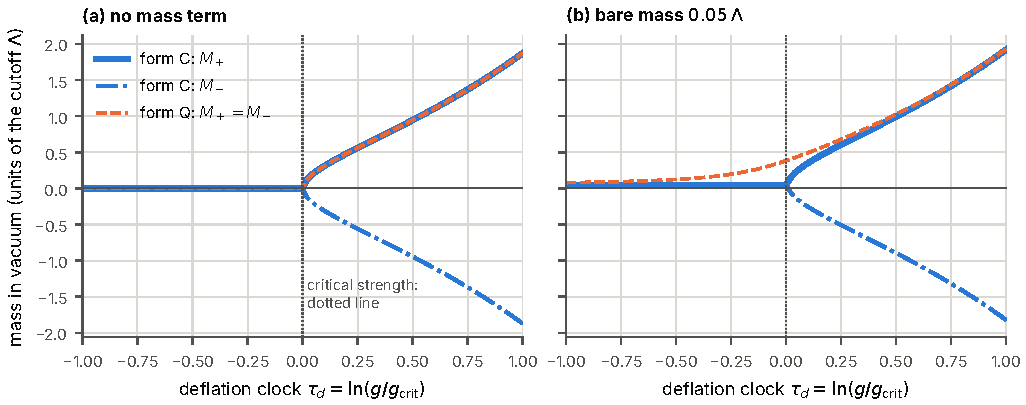
\includegraphics[width=0.86\textwidth]{fig_forms_vacuum}
\caption{\label{fig:vachalves}The masses of the particles of the two halves in vacuum with the filled
states of negative energy, along the clock counted from the critical strength of a massless field
(dotted line; $D=4$, set A; units of the cutoff). (a) A field without mass term: above the critical
strength form Q gives both halves the same mass, form C gives them masses of opposite sign. (b) With
the bare mass $0.05\,\Lambda$: form Q passes smoothly through the critical strength; in form C the
two masses are equal up to a sharp transition and separate there.}
\end{figure*}

\emph{The thresholds of Sec.~\ref{sec:ks} and the vacuum.} The calculation of Sec.~\ref{sec:ks}
without the filled states is consistent only while the vacuum is stable, that is, while the most
attractive scalar coupling is weaker than $G_c$ for the cutoff of the model. The last column of
Table~\ref{tab:ksthr} gives the largest cutoff for which this holds at the binding threshold. It is
below the mass in all eight cases, and smaller in form C than in form Q, because form C needs
stronger couplings to bind matter: \emph{in both forms, and more so in form C, self-bound matter by
contact couplings alone presupposes a cutoff below the mass of the particles.} How the filled states
change a saturation point when they are included was computed for an example of one kind of
particle on the $7{+}1$ spacetime ($D=7$), with the bare mass adjusted so that the mass in vacuum
stays the same: the saturation point moves little while the cutoff stays below about half the mass
in vacuum, and the binding grows for larger cutoffs [Fig.~\ref{fig:cjtsea}(b)]. The results of
Sec.~\ref{sec:ks} are therefore those of an effective theory with a low cutoff.

\subsection{Bare mass, self-interaction and Vorton-Scalar together}
\label{sec:unified}

Now let all terms of the model (\ref{eq:LVS}) act together, for fields in ordinary space ($D=3$) and
without the filled states. Let $\phi$ be the expectation value of the Vorton-Scalar,
$\langle\PhiVS\rangle=\phi/\sqrt2$, and $x=\phi/\vVS$. The mass of a fermion in a region with the
expectation value $\phi$ is $m_D+m_Y\,x$; let $f_D=m_D/m$ be the fraction of the mass in vacuum that
is a bare Dirac mass. In units $m=1$ the energy density of matter of the Fermi momentum $\kF$ is the
stationary value of
\begin{equation}
\begin{aligned}
\varepsilon={}&\frac{(1-f_D)^{2}\,(x^{2}-1)^{2}}{8\,C}+\langle E^{*}\rangle+\tfrac12\GV\,n^{2}\\
&-\frac{\big[\mst-f_D-(1-f_D)\,x\big]^{2}}{2\,\GS}
\end{aligned}
\label{eq:unified}
\end{equation}
with respect to $x$ and $\mst$: the first term is the potential of the scalar, with the number $C$
of Eq.~(\ref{eq:DC}); the others are Eq.~(\ref{eq:epsKS}) with the mass $f_D+(1-f_D)x$ in place of
$m$. Equation~(\ref{eq:unified}) is written for one kind of particle; for the two halves of the
field the last three terms are replaced by the energy density (\ref{eq:epshalves}) with
$f_D+(1-f_D)x$ in place of $m$, because the Yukawa coupling shifts the masses of both halves alike
(Sec.~\ref{sec:clock}). For $f_D=0$ and $\GS=\GV=0$ this is the functional of Sec.~\ref{sec:cjt}, and the program
reproduces its masses and energies to $2.1\times10^{-8}$ and its binding threshold
$C=3\pi^{2}/8$.

\emph{At low density the Vorton-Scalar acts as a scalar contact coupling.} Expanding
Eq.~(\ref{eq:unified}) for small densities gives $\mst=m+(\GS-C/m^{2})\,\nS$: the exchange of the
radial mode adds $-\gVS^{2}/m_s^{2}$ to the scalar coupling, whatever fraction of the mass is a bare
mass (verified for five sets of parameters to $1.8\times10^{-4}$ at Fermi momenta up to a
twentieth of $m$). The scalar
channel of the self-interaction and the exchange of the radial mode are the same interaction at
momenta far below $m_s$; they differ at higher densities, where the scalar field itself changes. For
the two halves this means that the Vorton-Scalar adds $-C/m^{2}$ to the coupling $\GStot$ of the
total scalar density, in both forms.

\emph{The moment at which matter becomes self-bound.} All couplings grow as $e^{\td}$, so that their
ratios are fixed and the deflation carries matter through a sequence of states with growing $C$.
Table~\ref{tab:unified} gives the smallest $C$ at which matter is self-bound in the two forms, for
contact couplings $g_0<0$ and $g_1>0$ of the Lagrangian proportional to $C$, and the shift of that
moment relative to the model with the Vorton-Scalar alone. \emph{A bare Dirac mass makes matter bind
earlier}, by 0.39 units of the clock if a quarter of the mass is a bare mass and by
0.58 if half of it is: the matter no longer has to pay for the destruction of the
whole expectation value of the scalar. In all 18 cases of the table the bound state at
the threshold has equal halves, in both forms: the attraction that binds it is that of the scalar
field, which acts on both halves alike, and contact couplings of these strengths are too weak to
polarize it. The threshold is that of matter of one kind with the couplings $\GStot$, $\GVtot$ of the
form, confirmed with the functional of two halves minimized over the density, the field and the
polarization. The forms differ because the couplings of the total densities differ
(Table~\ref{tab:kscoup}). In form Q the scalar contact coupling adds its attraction
$\GS^{\mathrm{HF}}$ to that of the scalar field, and a vector coupling adds the repulsion
$\GV^{\mathrm{HF}}$ [Fig.~\ref{fig:unified}(a,b), drawn against the mean-field couplings of matter of
one kind]. In form C the couplings of the total densities are $\GS^{\mathrm c}$ and
$\GV^{\mathrm c}$, both small, so that the contact couplings change the threshold less; which form
binds earlier depends on the case. Without bare mass the bound state of form C at the threshold
consists of massless particles ($x=0$), whose scalar densities vanish, and the threshold does not
depend on the vector coupling of the table.

\begin{table*}
\caption{\label{tab:unified}Bare Dirac mass, contact couplings and Vorton-Scalar together in the two
forms ($D=3$, without the filled states): the smallest $C$ at which uniform matter is self-bound,
in parentheses the shift of the moment of binding along the deflation clock relative to the first
row (negative: earlier), and the value $x$ of the scalar field in the bound state just above the
threshold.}
\begin{ruledtabular}
\begin{tabular}{ccccccc}
$f_D$ & $-g_0/C$ & $g_1/C$ & form C: $C$ ($\Delta\td$) & $x$ & form Q: $C$ ($\Delta\td$) & $x$ \\
\hline
0 & 0 & 0 & 3.7011 ($0$) & 0.000 & 3.7011 ($0$) & 0.000 \\
0 & 1 & 0 & 3.9399 ($+0.063$) & 0.000 & 3.7156 ($+0.004$) & 0.614 \\
0 & 1 & 0.1 & 3.9399 ($+0.063$) & 0.000 & 4.1527 ($+0.115$) & 0.652 \\
0.25 & 0 & 0 & 2.5112 ($-0.388$) & 0.000 & 2.5112 ($-0.388$) & 0.000 \\
0.25 & 1 & 0 & 2.6336 ($-0.340$) & 0.000 & 2.4758 ($-0.402$) & 0.000 \\
0.25 & 1 & 0.1 & 2.6307 ($-0.341$) & 0.000 & 2.6992 ($-0.316$) & 0.000 \\
0.5 & 0 & 0 & 2.0643 ($-0.584$) & 0.000 & 2.0643 ($-0.584$) & 0.000 \\
0.5 & 1 & 0 & 2.1617 ($-0.538$) & 0.000 & 1.8252 ($-0.707$) & 0.000 \\
0.5 & 1 & 0.1 & 2.1559 ($-0.540$) & 0.000 & 1.9335 ($-0.649$) & 0.000 \\
\end{tabular}
\end{ruledtabular}
\end{table*}

\begin{figure*}
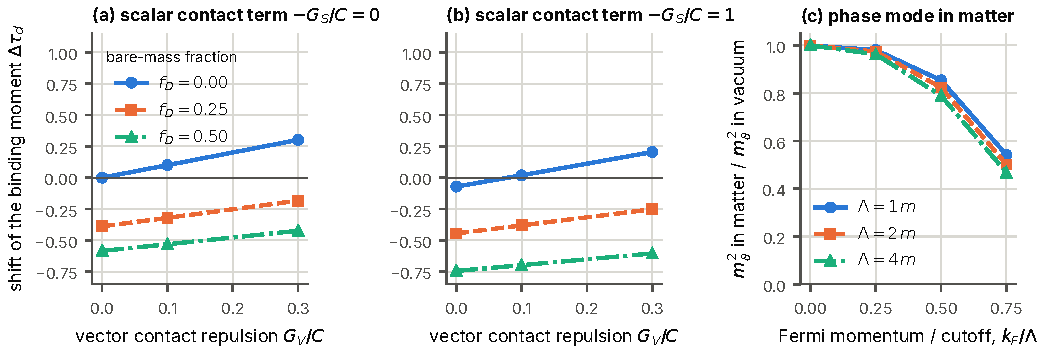
\includegraphics[width=\textwidth]{fig_unified}
\caption{\label{fig:unified}Bare Dirac mass, contact couplings and Vorton-Scalar together. (a), (b)
The shift of the moment at which matter becomes self-bound, in units of the deflation clock, against
the vector contact coupling, for three fractions $f_D$ of bare mass, without and with a scalar
contact coupling. (c) The square of the mass of the phase mode in matter divided by its value in
vacuum, against the Fermi momentum in units of the cutoff.}
\end{figure*}

\subsection{The mass of the phase mode}
\label{sec:phasemass}

A bare Dirac mass breaks the chiral symmetry $\UVS$ explicitly, and the phase mode of the
Vorton-Scalar is then no longer massless. Write $\PhiVS=(\vVS/\sqrt2)\,e^{i\vartheta_{\mathrm{VS}}}$
with a constant phase $\vartheta_{\mathrm{VS}}$. The mass term of the fermions becomes
$m_D+m_Y\,e^{i\vartheta_{\mathrm{VS}}\chi}$, the mass of a particle
\begin{equation}
m(\vartheta_{\mathrm{VS}})=\sqrt{m_D^{2}+m_Y^{2}+2\,m_Dm_Y\cos\vartheta_{\mathrm{VS}}},
\end{equation}
largest at $\vartheta_{\mathrm{VS}}=0$. The energy of the filled states of negative energy is lowest
where the mass is largest, so that the vacuum selects $\vartheta_{\mathrm{VS}}=0$, and the second
derivative of the energy density with respect to the phase is $\mth^{2}\vVS^{2}$. With
$dm/d\vartheta_{\mathrm{VS}}=0$ and $d^{2}m/d\vartheta_{\mathrm{VS}}^{2}=-m_Dm_Y/m$ at
$\vartheta_{\mathrm{VS}}=0$, and with the derivative of the energy density with respect to the mass,
which is the scalar density,
\begin{equation}
\mth^{2}\,\vVS^{2}=\Big(\big|\langle\bar\psi\psi\rangle_{\mathrm{vac}}\big|-\nS\Big)\,\frac{m_D\,m_Y}{m} .
\label{eq:mtheta}
\end{equation}
In vacuum ($\nS=0$) this is the relation of Gell-Mann, Oakes and Renner \cite{GellMannOakesRenner1968}
for the model at hand: the square of the mass of the phase mode is proportional to the bare mass and
to the scalar density of the vacuum. In ordinary space
$|\langle\bar\psi\psi\rangle_{\mathrm{vac}}|=(\nu m/4\pi^{2})\,[\Lambda\sqrt{\Lambda^{2}+m^{2}}-m^{2}\,\mathrm{arsinh}(\Lambda/m)]$;
the program confirms Eq.~(\ref{eq:mtheta}) against the numerical second derivative of the energy in
24 cases to $3.2\times10^{-7}$ of the value in vacuum. Three consequences follow.

\emph{The phase mode becomes heavier along the clock.} In the couplings of the model,
$\mth^{2}=C\,m_s^{2}\,f_D\,(|\langle\bar\psi\psi\rangle_{\mathrm{vac}}|-\nS)/[(1-f_D)\,m^{3}]$, which
grows as $e^{\td}$: $\mth\propto e^{\td/2}$, while all other masses stay fixed. Its value depends on
the cutoff through the scalar density of the vacuum (Table~\ref{tab:phasemode}).

\emph{In matter the phase mode is lighter.} The matter subtracts its scalar density:
$\mth^{2}(\kF)/\mth^{2}(0)=1-\nS/|\langle\bar\psi\psi\rangle_{\mathrm{vac}}|$
[Table~\ref{tab:phasemode}, Fig.~\ref{fig:unified}(c)].

\emph{A massive phase mode binds pairs less.} The exchange of the phase mode contributes to the
pairing potential (\ref{eq:VVS}) with the range $1/\mth$; a mass of three tenths of the fermion
mass reduces the gap of the example of Table~\ref{tab:gapcontact} ($m_s=m$) from
0.0247 to 0.0197 of the Fermi kinetic energy.

\begin{table}
\caption{\label{tab:phasemode}The phase mode of the Vorton-Scalar when a tenth of the fermion mass
is a bare Dirac mass ($f_D=0.1$; $D=3$; units $m=1$): scalar density of the vacuum, square of the
mass of the phase mode in vacuum in units of $C\,m_s^{2}$, and its reduction in matter of the Fermi
momenta $\Lambda/4$, $\Lambda/2$ and $3\Lambda/4$.}
\begin{ruledtabular}
\begin{tabular}{cccccc}
$\Lambda$ & $|\langle\bar\psi\psi\rangle_{\mathrm{vac}}|$ & $\mth^{2}/(C\,m_s^{2})$ & $\kF=\Lambda/4$ & $\Lambda/2$ & $3\Lambda/4$ \\
\hline
1 & 0.1080 & 0.0120 & 0.981 & 0.854 & 0.541 \\
2 & 0.6137 & 0.0682 & 0.974 & 0.824 & 0.502 \\
4 & 2.9176 & 0.3242 & 0.963 & 0.790 & 0.467 \\
\end{tabular}
\end{ruledtabular}
\end{table}

\section{Order parameter, hidden symmetry and vortices}
\label{sec:order}

\subsection{Frame components and coordinate components}

The order parameter of the superfluid is the expectation value $\Delta^{a}$ of the vector pair
operator (\ref{eq:pairs}) along the extra axis $a\in\{0,5,6,7\}$: four complex numbers. On the
deflating spacetime the index $a$ is a \emph{frame} index: $\Delta^{a}$ is the component along the
unit vector $e_a$. The coordinate components along the deflating coordinates are
$\Delta_t=b_t(x4)\,\Delta^{t}$, and they shrink with the scale factors when the frame components are
constant. All statements below are about frame components.

The energy of the paired state depends on the order parameter through the $8\times8$ gap matrix
$\MM$ on the internal states of a pair. The identity
\begin{equation}
\tfrac18\,\mathrm{Tr}\big[(\MM\MM^\dagger)^{2}\big]
=2\Big(\sum_a|\Delta^{a}|^{2}\Big)^{2}-\Big|\sum_{a,b}\eta_{ab}\,\Delta^{a}\Delta^{b}\Big|^{2},
\label{eq:quartic}
\end{equation}
holds on the deflating spacetime with the frame metric $\eta_{ab}$ of the four axes, to
$2\times10^{-14}$. In coordinate components the same expression contains the metric $g_{tt}$ of the
moment.

\subsection{The ground state: no direction is preferred}

\begin{table}
\caption{\label{tab:states}The potential $V$ of the paired state for six states of the order
parameter, in units of $N(0)\Delta_F^{2}$, where $\Delta_F$ is the gap of a unitary state. Each
state is taken at the magnitude of the order parameter at which its potential is stationary.
$d_-^{2}$ and $d_+^{2}$: the squares of the two fourfold gaps of the state, in units of
$\Delta_F^{2}$. Flat and positive: the numbers of eigenvalues of the matrix of second derivatives of
the potential that vanish and that are positive.}
\begin{ruledtabular}
\begin{tabular}{p{0.37\columnwidth}ccccc}
state & $d_-^{2}$ & $d_+^{2}$ & $V$ & flat & positive \\
\hline
pair along the frame axis of $x0$ (hidden-axis singlet) & 1.000 & 1.000 & $-2.0000$ & 4 & 4 \\
pair along the frame axis of $x5$ & 1.000 & 1.000 & $-2.0000$ & 4 & 4 \\
pair along the frame axis of $x7$ & 1.000 & 1.000 & $-2.0000$ & 4 & 4 \\
unitary, rotated between $x0$ and $x5$ & 1.000 & 1.000 & $-2.0000$ & 4 & 4 \\
unitary, general direction and phase & 1.000 & 1.000 & $-2.0000$ & 4 & 4 \\
half-paired: $\eta_{ab}\Delta^a\Delta^b=0$ & 0.000 & 1.000 & $-1.0000$ & --- & --- \\
\end{tabular}
\end{ruledtabular}
\end{table}

Table~\ref{tab:states} gives the potential of the paired state for six states of the order
parameter. Every \emph{unitary} state, in which $\Delta^{a}$ is a real unit vector times a phase, has
all eight gaps equal and the lowest potential, whichever direction the vector has. It has four flat
directions, the Goldstone modes (one phase and three rotations of the direction), and four
directions of positive curvature. The \emph{half-paired} states, in which four of the eight gaps
vanish, have half the condensation energy.

One might have expected the deflation to select the direction of the order parameter: the hidden
axis $x0$, which does not deflate, against the three axes that do. \emph{In the sector of fields
that do not depend on the extra coordinates it does not.} The reason is the central observation of
Sec.~\ref{sec:dirac}: in this sector the weighted field obeys the flat equations, and their internal
symmetry rotates the four frame axes into one another. The symmetry of the manifold of ground states
is larger than the symmetry of the spacetime.

This holds for the model without contact self-interaction, for which Table~\ref{tab:states} is
computed, and for a self-interaction of form Q. \emph{A self-interaction of form C, the definition
of the model, does select a direction.} It breaks the three generators that rotate the hidden axis
into $x5,x6,x7$ (Sec.~\ref{sec:selfsym}), and it enters the pair along the hidden axis and the pairs
along $x5,x6,x7$ with opposite signs, so that their gaps differ (Sec.~\ref{sec:gapformc}). What
selects the direction is the self-interaction, through the distinction that the signature of the
spacetime makes between the space-like hidden axis and the additional times; the deflation still
selects nothing, because it does not act in this sector. The three flat directions of
Table~\ref{tab:states} that rotate the hidden axis into the other three are then no longer flat. The
potential of the order parameter with the contact couplings of form C has not been computed.

\subsection{The internal symmetry of the sector, and the symmetries of the spacetime}
\label{sec:hidden}

For fields that depend on $x1,x2,x3,x4$ only, the equation of the weighted field contains five
matrices: $\alpha^{1},\alpha^{2},\alpha^{3}$, $\beta$ and $i\beta\chi$, the last through the coupling of the phase mode. The matrices that commute
with all five generate the \emph{internal symmetry} of the sector. The program computes it again for
the deflating spacetime, item by item (Table~\ref{tab:xsymmetry}), and finds it unchanged:
\begin{itemize}
\item the algebra is $su(2)_A\oplus su(2)_B\oplus u(1)_F\oplus u(1)_E$, of dimension 8;
\item the eight internal states of a fermion form the two doublets $(2,1)+(1,2)$;
\item the four vector pair operators (\ref{eq:pairs}) form the $(2,2)$, with fermion number 2, and
their one invariant quadratic form is the frame metric of the four axes, with the signs
$(+,-,-,-)$;
\item a condensate along one axis breaks $SO(4)=[SU(2)_A\times SU(2)_B]/Z_2$ to $SO(3)$.
\end{itemize}
Here $U(1)_E$ is a second phase symmetry of the sector, with a generator $P$ that has the square one
and distinguishes the doublets of $SU(2)_A$ from those of $SU(2)_B$.

Six of the generators are the products $\gamma^{A}\gamma^{B}$ of the six pairs taken from the four
axes $x0,x5,x6,x7$.
On the flat $4{+}4$ spacetime only three of them belong to transformations of the spacetime that the
sector inherits: the products $\gamma^{s}\gamma^{t}$ of two additional times generate the rotations
$SO(3)_T$ of $x5,x6,x7$. The other three, $\gamma^{0}\gamma^{t}$, are Hermitian; the unitary
transformations that they generate in the quantized sector are not the boosts of the planes of $x0$
and $xt$, which are not unitary. The full $SU(2)_A\times SU(2)_B$ was therefore a \emph{hidden
symmetry} already on the flat spacetime: a symmetry of the equations of a sector that is not a
transformation of the spacetime. On the deflating spacetime even $SO(3)_T$ is a
symmetry of the spacetime only if the three rates are equal (Fig.~\ref{fig:isometries}). With two
equal rates one rotation remains, and with three different rates none. The internal symmetry of the
sector is nevertheless exact in all three cases.

\subsection{Vortices and their zero modes}
\label{sec:vortex}

Because the vacuum value of the Vorton-Scalar breaks the phase symmetry $\UVS$, the field has
line-like defects \cite{NielsenOlesen1973}: along a straight line, say the $x3$ axis, its magnitude
vanishes, and around the line its phase winds by $2\pi$ times an integer. For unit winding,
$\PhiVS$ is $\vVS/\sqrt2$ times a profile that rises from 0 on the line to 1 at a distance of the
order of $1/m_s$, times $e^{i\theta_{12}}$ with the angle $\theta_{12}$ around the line in the plane
of $x1$ and $x2$.

\emph{Energy per unit length.} It is proportional to the square of the four-dimensional vacuum
value and so falls as $e^{-\td}$: in the four-dimensional description vortex lines become lighter as
the deflation proceeds, while their core, of the radius $1/m_s$, keeps its size.

\emph{Fermions on the line.} On the line the fermion mass vanishes, and fermions can be trapped
there \cite{JackiwRossi1981}. In the field of the vortex the Hamiltonian of a fermion is
\begin{equation}
\sum_{j=1}^{3}\alpha^{j}p_j+m\,(\text{profile})\,\beta\,\big(\cos\theta_{12}+i\chi\,\sin\theta_{12}\big),
\end{equation}
with the momenta $p_j$ along $x1,x2,x3$. A state of zero energy at zero momentum along the line is a
constant spinor $w_z$ times a function that decays away from the line. Inserting this form, the
Hamiltonian annihilates the state for every angle if and only if
\begin{equation}
\big(i\alpha^{1}+\beta\big)\,w_z=0,\qquad\big(i\alpha^{2}+i\beta\chi\big)\,w_z=0 .
\label{eq:zeromode}
\end{equation}
The five matrices $\alpha^{1},\alpha^{2},\alpha^{3},\beta,i\beta\chi$ are Hermitian, have the square
one and anticommute with one another. The two conditions state that $w_z$ is an eigenvector, with the
eigenvalue $-1$, of the two commuting matrices $i\beta\alpha^{1}$ and $\alpha^{2}\beta\chi$, and each
joint eigenspace of these two matrices has the dimension $16/4=4$. \emph{A vortex line of unit
winding carries four zero modes of the sixteen-component field.}

For a momentum $p_3$ along the line the energy is the eigenvalue of $\alpha^{3}p_3$. On the four
zero modes $\alpha^{3}$ equals the matrix
\begin{equation}
P_c=i\,\alpha^{1}\alpha^{2}\alpha^{3}\chi,
\end{equation}
the product of the five matrices, which commutes with each of them, is Hermitian and traceless and
has the square one; it is, up to its sign, the generator $P$ of $U(1)_E$. Its trace on the four zero
modes vanishes. \emph{Two zero modes move along the line in one direction at the speed of light and
two in the other}, and the direction of motion is tied to the charge under $U(1)_E$. For winding $-1$
the two directions are exchanged.

Equations (\ref{eq:zeromode}) contain only the matrices of the frame and the fermion mass, neither of
which changes. The four zero modes therefore exist at every moment of the deflation. The count also
holds on flat spacetime. (The familiar count for a four-component field is one zero mode for each
unit of winding; the sixteen components are equivalent to four such fields.)

Massless fermions that run along a vortex line carry a current \cite{Witten1985}; a closed loop of
the line can be held open by that current, and such loops are the \emph{vortons} of the literature
on cosmic strings \cite{DavisShellard1989}. Because the energy per length of the line falls as
$e^{-\td}$ while the fermions on it stay massless, the balance between the tension of a loop and the
current on it shifts in favor of the current as the deflation proceeds. This paper establishes the
ingredients of that statement; it does not compute the equilibrium radius of a loop.

\section{Gravity: the deflating spacetime with matter as its source}
\label{sec:gravity}

The hypothesis (\ref{eq:hyp}) prescribes the metric. This section asks what the field equations of
gravity make of it when the matter of Sec.~\ref{sec:ks} is their source: whether such matter can
produce the deflation, and what it does to a deflation that is already under way.

\subsection{Two scale factors and the Einstein-Lovelock equations}

Let the three rates be equal, and let the four flat coordinates have a scale factor of their own:
\begin{equation}
ds^{2}=-(dx4)^{2}+\ma(x4)^{2}\sum_{j=0}^{3}(dxj)^{2}-\mb(x4)^{2}\sum_{t=5}^{7}(dxt)^{2},
\label{eq:twofactors}
\end{equation}
with the rates $H_{\ma}=\ma'/\ma$ and $H_{\mb}=\mb'/\mb$ (a prime is a derivative with respect to
$x4$). The deflating spacetime of the hypothesis is $\ma=1$, $\mb=\cff\,e^{-\gff\,x4}$, that is,
$H_{\ma}=0$ and $H_{\mb}=-\gff$; it is called the \emph{undisturbed deflation} below.

For a metric of this kind the Riemann tensor is determined by one number for each pair of
directions of the frame, the sectional curvature of their plane (Appendix~\ref{app:curvature}):
\begin{equation}
K_{4i}=H_i'+H_i^{2},\qquad K_{ij}=H_i\,H_j\quad(i\ne j),
\label{eq:paircurv}
\end{equation}
where $i,j$ run over the seven directions other than the time and $H_i$ is the rate of the
direction $i$. The same formulas hold for the time-like directions $x5,x6,x7$ of the $4{+}4$
spacetime, so that everything that follows is the same on the $4{+}4$ and on the $7{+}1$
spacetime.The field equations of second order for the metric in eight dimensions are those of
Lovelock \cite{Lovelock1971}, with tensors $E^{(k)\mu}{}_{\nu}$ of the orders $k=1,2,3$ in the
curvature. For the metric (\ref{eq:twofactors}) they are diagonal, and
\begin{equation}
E^{(k)m}{}_{m}=(-1)^{k+1}\,k!\,2^{k-1}\!\!\sum_{\substack{\text{sets of }2k\\ \text{directions}\ne m}}\ \sum_{\substack{\text{divisions}\\ \text{into pairs}}}\ \prod_{\text{pairs}}K_{\text{pair}} ,
\label{eq:lovelockE}
\end{equation}
without summation over $m$: the sum runs over all sets of $2k$ directions that do not contain $m$,
and over the ways to divide such a set into $k$ pairs (one way for $k=1$, three for $k=2$, fifteen
for $k=3$). In this notation and sign $E^{(1)\mu}{}_{\nu}=-\cG^{\mu}{}_{\nu}$ is minus the Einstein
tensor and $E^{(2)\mu}{}_{\nu}=\cH^{\mu}{}_{\nu}$ the Lanczos tensor of Sec.~\ref{sec:egb}. The
\emph{Einstein-Lovelock equations} are
\begin{equation}
\sum_{k=1}^{3}\alpha_k\,E^{(k)\mu}{}_{\nu}-\bar\Lambda\,\delta^{\mu}_{\nu}=\kappa_8\,T^{\mu}{}_{\nu},\qquad\alpha_1=1,
\label{eq:EL}
\end{equation}
with the couplings $\alpha_2$, $\alpha_3$ of the two higher terms, the cosmological term
$\bar\Lambda$, and the gravitational coupling $\kappa_8$ of the eight-dimensional theory. The
energy-momentum tensor of uniform matter has the components $T^{4}{}_{4}=\varepsilon$ and
$T^{m}{}_{m}=-p_m$, with the energy density and the pressures of Sec.~\ref{sec:ks}. [In terms of
Eq.~(\ref{eq:egb}): $\bar\Lambda=\Lam$ and $\alpha_2=-\aGB$.]

Written out for four directions with the rate $H_{\ma}$ and three with the rate $H_{\mb}$, the
first two orders are
\begin{equation}
\begin{aligned}
E^{(1)4}{}_{4}={}&6H_{\ma}^{2}+12H_{\ma}H_{\mb}+3H_{\mb}^{2},\\
E^{(1)\ma}{}_{\ma}={}&3H_{\ma}'+3H_{\mb}'+6H_{\ma}^{2}+9H_{\ma}H_{\mb}+6H_{\mb}^{2},\\
E^{(1)\mb}{}_{\mb}={}&4H_{\ma}'+2H_{\mb}'+10H_{\ma}^{2}+8H_{\ma}H_{\mb}+3H_{\mb}^{2},
\end{aligned}
\label{eq:E1}
\end{equation}
\begin{equation}
\begin{aligned}
E^{(2)4}{}_{4}={}&-12H_{\ma}^{4}-144H_{\ma}^{3}H_{\mb}-216H_{\ma}^{2}H_{\mb}^{2}\\
&-48H_{\ma}H_{\mb}^{3},\\
E^{(2)\ma}{}_{\ma}={}&-12\big(H_{\ma}^{2}+6H_{\ma}H_{\mb}+3H_{\mb}^{2}\big)H_{\ma}'\\
&-12\big(3H_{\ma}^{2}+6H_{\ma}H_{\mb}+H_{\mb}^{2}\big)H_{\mb}'\\
&-12H_{\ma}^{4}-108H_{\ma}^{3}H_{\mb}-180H_{\ma}^{2}H_{\mb}^{2}\\
&-108H_{\ma}H_{\mb}^{3}-12H_{\mb}^{4},\\
E^{(2)\mb}{}_{\mb}={}&-16\big(3H_{\ma}^{2}+6H_{\ma}H_{\mb}+H_{\mb}^{2}\big)H_{\ma}'\\
&-16\big(3H_{\ma}^{2}+2H_{\ma}H_{\mb}\big)H_{\mb}'-60H_{\ma}^{4}\\
&-192H_{\ma}^{3}H_{\mb}-136H_{\ma}^{2}H_{\mb}^{2}-32H_{\ma}H_{\mb}^{3},
\end{aligned}
\label{eq:E2}
\end{equation}
where the index $\ma$ ($\mb$) stands for any one of the four (three) directions. Every term of the
third order contains at least two factors of $H_{\ma}$ or of its derivative, for example
$E^{(3)4}{}_{4}=1080H_{\ma}^{4}H_{\mb}^{2}+1440H_{\ma}^{3}H_{\mb}^{3}$. The component along the time
contains no derivative of a rate: it is a \emph{constraint} on the initial data. The two other
components are linear in $H_{\ma}'$ and $H_{\mb}'$ and are solved for them at every step of an
integration. The polynomials (\ref{eq:E1}) and (\ref{eq:E2}) were obtained by the program from
Eq.~(\ref{eq:lovelockE}) and, independently, by computer algebra in two ways: from the Riemann
tensor of the metric, and as the Euler-Lagrange equations of the reduced action for the lapse and
the two scale factors.

\subsection{A reference calculation}

The program was tested on a calculation done before with other tools: gravity with three
coordinates of ordinary space (scale factor $\ma$) and four further space coordinates (scale factor
$\mb$), driven by the matter of the reference example of
the $7{+}1$ spacetime ($D=7$, $\GS=-10^{5}$, $\GV=+10^{4}$ in units $m=1$, at its saturation
density), with $\kappa_8=1000$, $\bar\Lambda=0$,
$H_{\ma}(0)=0.05$ and $\ma(0)=\mb(0)=1$, integrated to $x4=20$ in Einstein gravity and in
Einstein-Lovelock gravity with $\alpha_2=20$, $\alpha_3=500$. The constraint gives $H_{\mb}(0)$. The
ten numbers of the first calculation are reproduced to $4.8\times10^{-8}$ by the program and by
the independent script (Table~\ref{tab:gravref}, Fig.~\ref{fig:gravref}); the constraint is
preserved along the integration to $1.3\times10^{-14}$.

\begin{table}
\caption{\label{tab:gravref}The reference calculation: three space coordinates with the scale factor
$\ma$ and four with the scale factor $\mb$, with matter of seven space dimensions as the source
(units $m=1$). EL: Einstein-Lovelock gravity with $\alpha_2=20$, $\alpha_3=500$.}
\begin{ruledtabular}
\begin{tabular}{llll}
gravity & quantity & this program & first calculation \\
\hline
Einstein & $H_{\mathsf b}(0)$ & 0.00914371 & 0.00914371 \\
Einstein & $\mathsf a(20)$ & 1.58173868 & 1.58173870 \\
Einstein & $\mathsf b(20)$ & 1.19755856 & 1.19755860 \\
Einstein & $H_{\mathsf a}(20)$ & 0.01187800 & 0.01187800 \\
Einstein & $H_{\mathsf b}(20)$ & 0.00741911 & 0.00741911 \\
EL & $H_{\mathsf b}(0)$ & 0.01498070 & 0.01498070 \\
EL & $\mathsf a(20)$ & 1.47735148 & 1.47735150 \\
EL & $\mathsf b(20)$ & 1.27608405 & 1.27608410 \\
EL & $H_{\mathsf a}(20)$ & 0.01017591 & 0.01017591 \\
EL & $H_{\mathsf b}(20)$ & 0.00848876 & 0.00848876 \\
\end{tabular}
\end{ruledtabular}
\end{table}

\begin{figure*}
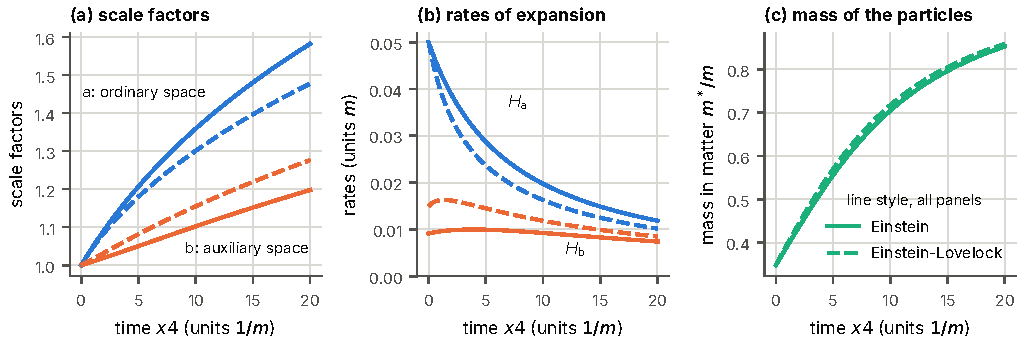
\includegraphics[width=\textwidth]{fig_gravity_reference}
\caption{\label{fig:gravref}The reference calculation of Table~\ref{tab:gravref}: (a) the two scale
factors, (b) their rates, (c) the mass of the particles in the matter, which rises as the matter is
diluted. Solid lines: Einstein gravity; dashed lines: Einstein-Lovelock gravity.}
\end{figure*}

\subsection{The undisturbed deflation as a solution}

\emph{Without matter.} For $H_{\ma}=0$, $H_{\mb}=-\gff$ and constant rates,
Eqs.~(\ref{eq:E1}) and (\ref{eq:E2}) give
$E^{(1)4}{}_{4}=3\gff^{2}$, $E^{(1)\ma}{}_{\ma}=6\gff^{2}$, $E^{(1)\mb}{}_{\mb}=3\gff^{2}$,
$E^{(2)\ma}{}_{\ma}=-12\gff^{4}$, and zero for the other components. The three equations
(\ref{eq:EL}) without matter hold if and only if
\begin{equation}
\bar\Lambda=3\,\gff^{2},\qquad\alpha_2=\frac{1}{4\,\gff^{2}},
\label{eq:tuned}
\end{equation}
which is Eq.~(\ref{eq:egbsol}); $\alpha_3$ is arbitrary. The gravity with these two constants is
called the \emph{tuned} Einstein-Lovelock gravity below. At this solution the coefficients of
$(H_{\ma}',H_{\mb}')$ in the two evolution equations form the matrix $\mathrm{diag}(-6,2)$, which
can be inverted: the evolution of a perturbed solution is well defined.

\emph{In Einstein gravity.} Without the Gauss-Bonnet term and without $\bar\Lambda$ the same
spacetime requires a source with
\begin{equation}
\kappa_8\,\varepsilon=3\,\gff^{2},\qquad p_{\ma}=-2\,\varepsilon,\qquad p_{\mb}=-\varepsilon ,
\label{eq:agent}
\end{equation}
a tension along the flat coordinates twice as large as the energy density, and a tension along the
deflating coordinates equal to it. \emph{The matter of Sec.~\ref{sec:ks} cannot be this source.} Its
pressure along a coordinate on which the fields do not depend is the interaction pressure $\pint$ of
Eq.~(\ref{eq:pKS}), and $\varepsilon+\pint=\langle E^{*}\rangle+\GV\,n^{2}$, which is positive for a
repulsive or vanishing vector coupling (for the two halves of the field,
$\varepsilon+\pint=\sum_\pm\langle E^{*}_\pm\rangle+\GVtot\,n^{2}+\GVdif\,n_W^{2}$, which is positive for
the sets A and B in both forms); $p_{\mb}=-\varepsilon$ is not reached. Something else must
hold the deflation: an \emph{agent} with the equation of state (\ref{eq:agent}), or the tuned
Gauss-Bonnet term.

\subsection{Matter on the deflating spacetime}

Now let matter be present, with the initial data $\ma=\mb=1$, $H_{\ma}=0$, and $H_{\mb}$ from the
constraint. Its amount is given by the \emph{loading}, $\kappa_8\,\varepsilon(0)/(3\,\gff^{2})$, the
energy density at the start in units of the energy density that would make three coordinates
deflate at the rate $\gff$ in Einstein gravity. The rate is $\gff=0.01\,m$.
The matter is that of the quantized sector, whose fields do not depend on $x5,x6,x7$ ($D=4$):
self-bound matter of set B at three times its binding threshold, at its saturation density, in the
two forms (Table~\ref{tab:gravmatter}). In form C one half of the field is filled, in form Q both
halves equally. In an evolution without collisions every particle keeps its state, so that a half
that is empty stays empty: the matter of form C is then matter of one kind of particle with four
internal states and the couplings $\GSsame$, $\GVsame$ throughout the evolution, and the matter of
form Q is matter of one kind with eight states and the couplings $\GS^{\mathrm{HF}}$,
$\GV^{\mathrm{HF}}$ (both were computed again with the routines for matter of one kind, with
agreement to $1.3\times10^{-15}$). The pressure along the deflating coordinates is $\pint$. The integration
runs until the clock of the undisturbed deflation, $\td^{0}=3\,\gff\,x4$, reads 6, or until a rate
exceeds $50\,\gff$ (Table~\ref{tab:gravdefl}, Fig.~\ref{fig:gravdefl}).

\begin{table}
\caption{\label{tab:gravmatter}The matter of the evolutions of Table~\ref{tab:gravdefl}: self-bound
matter of set B at three times the binding threshold of its form ($D=4$; units $m=1$). Second
column: the strength $g$ at the binding threshold. The Fermi momentum $k_{F+}$ and the mass $m^{*}_+$
are those of the filled half in form C (taken as the half $\Wg=+1$) and of each of the two halves in
form Q.}
\begin{ruledtabular}
\begin{tabular}{cccccc}
form & $g\,m^{3}$ & state & $k_{F+}/m$ & $m^{*}_+/m$ & $\varepsilon/n-m$ \\
\hline
C & 332.2917 & one half filled & 0.52859 & 0.37920 & $-0.09072$ \\
Q & 121.0858 & equal halves & 0.58171 & 0.35844 & $-0.10601$ \\
\end{tabular}
\end{ruledtabular}
\end{table}

\begin{table*}
\caption{\label{tab:gravdefl}The deflating spacetime with matter as a source of gravity. Tuned EL:
Einstein-Lovelock gravity with the constants (\ref{eq:tuned}), in which the undisturbed deflation
is a solution without matter; Einstein: Einstein gravity with the matter as the only source. The
last five columns give the state at the end of the integration; ``runaway'' marks an evolution in
which a rate exceeded $50\,\gff$ before $\td^{0}=6$.}
\begin{ruledtabular}
\begin{tabular}{lllcllcccc}
matter & gravity & loading & $H_{\mb}(0)/\gff$ & end & $\td^{0}$ & $\ma$ & $\mb$ & $H_{\ma}/\gff$ & $H_{\mb}/\gff$ \\
\hline
$4{+}4$, form C & tuned EL & $10^{-3}$ & $-1.0005$ & reached & 6.00 & 1.5963 & 0.01521 & $+6.2500$ & $-34.104$ \\
$4{+}4$, form C & tuned EL & $10^{-1}$ & $-1.0488$ & runaway & 3.51 & 1.6307 & 0.02463 & $+9.1436$ & $-50.090$ \\
$4{+}4$, form C & Einstein & $10^{-3}$ & $-0.0316$ & reached & 6.00 & 1.0014 & 0.9332 & $+0.0015$ & $-0.038$ \\
$4{+}4$, form C & Einstein & $10^{-1}$ & $-0.3162$ & runaway & 4.01 & 1.5871 & 0.09687 & $+11.7156$ & $-50.030$ \\
$4{+}4$, form Q & tuned EL & $10^{-3}$ & $-1.0005$ & reached & 6.00 & 1.4087 & 0.02928 & $+2.8489$ & $-15.606$ \\
$4{+}4$, form Q & tuned EL & $10^{-1}$ & $-1.0488$ & runaway & 3.57 & 1.6321 & 0.02386 & $+9.1359$ & $-50.050$ \\
$4{+}4$, form Q & Einstein & $10^{-3}$ & $-0.0316$ & reached & 6.00 & 1.0015 & 0.9332 & $+0.0016$ & $-0.038$ \\
$4{+}4$, form Q & Einstein & $10^{-1}$ & $-0.3162$ & runaway & 4.02 & 1.6299 & 0.09367 & $+12.2541$ & $-50.124$ \\
\end{tabular}
\end{ruledtabular}
\end{table*}

\begin{figure*}
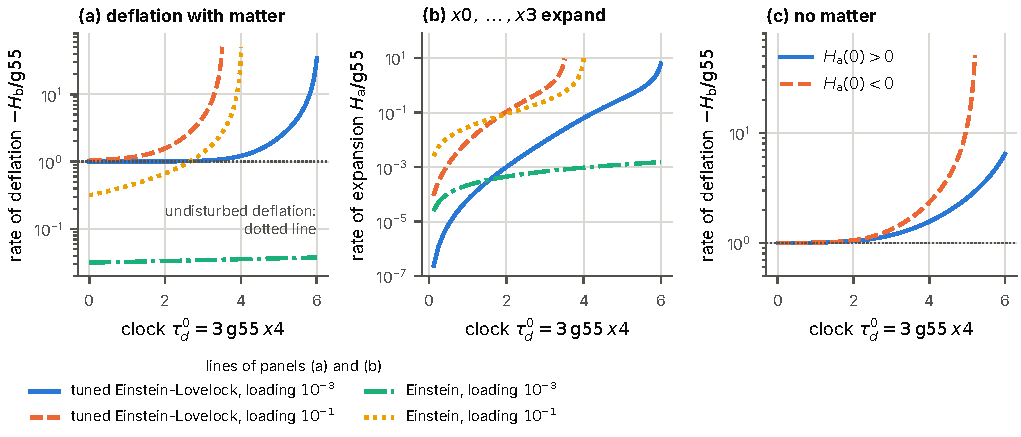
\includegraphics[width=\textwidth]{fig_gravity_deflating_formC}
\caption{\label{fig:gravdefl}The deflating spacetime with matter as a source of gravity
(matter of form C, one half of the field filled; the
runs of Table~\ref{tab:gravdefl}). (a) The rate of deflation $-H_{\mb}$ in units of $\gff$ against
the clock of the undisturbed deflation. (b) The rate $H_{\ma}$ at which the four flat coordinates
expand. (c) The tuned Einstein-Lovelock gravity without matter, started with a deflation one part in
a thousand faster than the undisturbed one: the two initial data that the constraint allows.}
\end{figure*}

\begin{figure*}
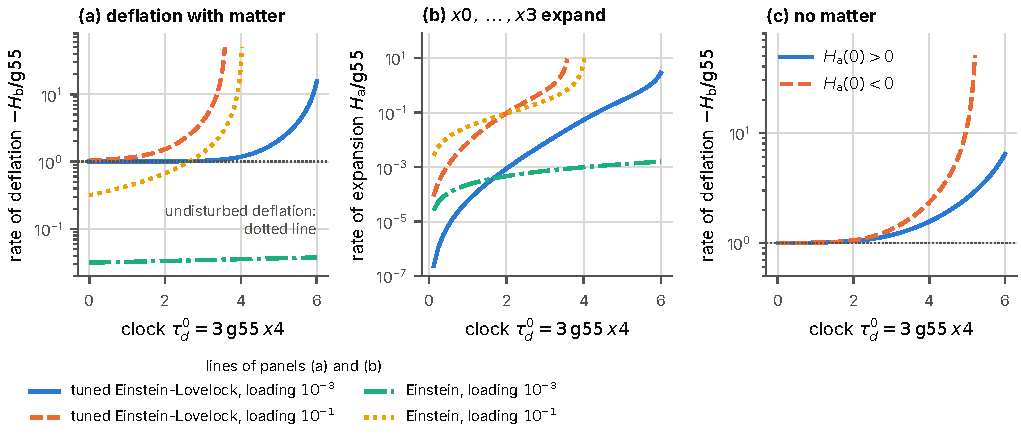
\includegraphics[width=\textwidth]{fig_gravity_deflating_formQ}
\caption{\label{fig:gravdeflQ}As Fig.~\ref{fig:gravdefl}, with the matter of form Q (both halves of
the field equally filled) as the source.}
\end{figure*}

\emph{Matter makes the deflation faster than exponential and makes the flat coordinates expand.} In
the tuned gravity the smaller loading leaves the deflation close to the undisturbed one for about
four units of the clock; then the rates grow, and at $\td^{0}=6$ the three coordinates deflate
34.1 times faster than at the start for the matter of form C, and
15.6 times for that of form Q, while the four flat
coordinates expand. With the larger loading the rates exceed $50\,\gff$ before the clock reads 4:
they grow without bound in a finite time. In Einstein gravity with the matter as the only source the
initial rate is $-H_{\mb}(0)=\gff\times(\text{loading})^{1/2}$, far below $\gff$ for a small loading,
and it grows as the matter is compressed. In four of
the eight evolutions of the table the rates run away. The two forms give matter of different
composition and behave alike in kind: the conclusions of this section do not depend on the form
(Fig.~\ref{fig:gravdeflQ} shows the evolutions with the matter of form Q). The constraint is preserved along
every evolution to $6.7\times10^{-10}$.

\subsection{The undisturbed deflation is unstable}

The behavior just described is not caused by the matter alone. Near the undisturbed deflation, with
$H_{\mb}=-\gff+\delta H_{\mb}$ and to the lowest order in $\delta H_{\mb}$, $H_{\ma}$ and the energy
density, the constraint of the tuned gravity reads
\begin{equation}
-6\,\gff\,\delta H_{\mb}-48\,H_{\ma}^{2}=\kappa_8\,\varepsilon .
\label{eq:constraint}
\end{equation}
The terms linear in $H_{\ma}$ cancel between the Einstein and the Gauss-Bonnet part, which is why
$H_{\ma}$ enters quadratically. Since $\varepsilon\ge0$, the left-hand side must not be negative:
\emph{initial data exist only for a deflation that is at least as fast as the undisturbed one},
$\delta H_{\mb}\le0$. For a deflation exactly at the rate $\gff$ and without matter the constraint is
$H_{\ma}^{2}\,(H_{\ma}^{2}-12\,\gff H_{\ma}+16\,\gff^{2})=0$, with the roots $0$, $0$ and
$(6\pm\sqrt{20})\,\gff$: the undisturbed deflation is a double root, on the edge of the allowed
initial data.

For a deflation faster by one part in a thousand and no matter, the constraint has the two roots
$H_{\ma}(0)=\pm\gff\,(0.001/8)^{1/2}$ to the lowest order. Starting from either, the deflation does
not return to the rate $\gff$: it becomes faster and faster
[Table~\ref{tab:gravvac}, Fig.~\ref{fig:gravdefl}(c)]. \emph{The exactly exponential deflation is an
unstable solution of the gravity in which it is a solution without matter}; every allowed
perturbation, with or without matter, grows.

\begin{table}
\caption{\label{tab:gravvac}The tuned Einstein-Lovelock gravity without matter, started at
$H_{\mb}(0)=-1.001\,\gff$ with the two values of $H_{\ma}(0)$ that the constraint allows: the state
at the end of the integration (at $\td^{0}=6$, or where a rate exceeded $50\,\gff$).}
\begin{ruledtabular}
\begin{tabular}{cccc}
$H_{\ma}(0)/\gff$ & $\td^{0}$ at the end & $H_{\ma}/\gff$ & $H_{\mb}/\gff$ \\
\hline
$+0.01147$ & 6.00 & $+1.7334$ & $-6.422$ \\
$-0.01088$ & 5.20 & $-0.0050$ & $-50.155$ \\
\end{tabular}
\end{ruledtabular}
\end{table}

Three conclusions follow for the hypothesis. First, the matter of the model does not produce the
deflation; an agent with the equation of state (\ref{eq:agent}), or a tuned Gauss-Bonnet term, is
needed. Second, with the Gauss-Bonnet term the deflation is not stable, so that the Gauss-Bonnet term
alone does not explain a deflation that lasts. Third, whatever holds the deflation must also absorb
the reaction of the matter, which pushes toward a faster deflation and an expansion of the flat
coordinates; the sections on cosmology assume such an agent and say so (assumption A2 of
Sec.~\ref{sec:cosmo}).

\section{Cosmology}
\label{sec:cosmo}

Hypothesis H3 says that the superfluid explains the dark matter, or the Hubble tension, or both. The
model offers a candidate for each. For the Hubble tension it is the phase mode of the Vorton-Scalar,
a massless boson that would act as radiation in addition to photons and neutrinos (\emph{dark
radiation}) and make the early universe expand faster. For the dark matter it is the fermions
themselves, as a degenerate gas or as a condensate of bound pairs. This section computes what each
candidate gives when $x5,x6,x7$ deflate; the case of static extra coordinates is the case of
vanishing rates, $\gsum=0$, and appears in every table below as the row or column without deflation.
The deflation enters cosmology in several ways, and each requires an assumption beyond the
hypothesis of deflation. The assumptions are stated first and are kept apart throughout, so that the
reader can see which conclusion rests on which.

\subsection{Assumptions, and the equation of the expansion}

\emph{A1: ordinary space expands.} The coordinates $x1,x2,x3$ carry the scale factor
$a_{\mathrm{sp}}(x4)$ of standard cosmology, with the Hubble rate $H=d\ln a_{\mathrm{sp}}/dx4$; the
hidden coordinate $x0$ is static; $x5,x6,x7$ deflate at constant rates. The metric of
Sec.~\ref{sec:geometry} is the case $a_{\mathrm{sp}}=1$.

\emph{A2: gravity is the Einstein theory in eight dimensions}, with a constant $G_8$. The constant
of gravitation that an observer in ordinary space measures is then $G_8$ divided by the proper volume
of the extra coordinates,
\begin{equation}
\GN(x4)\ \propto\ \frac{1}{\Vd}\ \propto\ e^{\gsum\,x4},\qquad\frac{1}{\GN}\frac{d\GN}{dx4}=\gsum .
\label{eq:GN}
\end{equation}
Newton's constant \emph{grows} as the extra volume shrinks: gravity was weaker in the past. That a
changing volume of extra dimensions makes the constants of four dimensions change, and that
nucleosynthesis bounds the change, was pointed out long ago \cite{KolbPerryWalker1986}; for a review
of varying constants see Ref.~\cite{Uzan2011}. By Sec.~\ref{sec:egb}, A2 is an assumption that the
deflating spacetime itself puts in doubt: without matter the metric solves the equations of
Einstein-Gauss-Bonnet gravity, not Einstein's.

For a diagonal metric whose seven directions other than the time have the rates $H,H,H$ (ordinary
space), $0$ (the coordinate $x0$) and $-\gff,-\gss,-\gvv$, the component of Einstein's equations
along the time is the sum of the products of all pairs of rates, set equal to $8\pi G_8$ times the
energy density in eight dimensions. Dividing the density by the extra volume turns $G_8$ into $\GN$:
\begin{equation}
3H^{2}-3\,\gsum\,H+\gprod=8\pi\,\GN(x4)\,\rho,
\label{eq:friedmann}
\end{equation}
with the density $\rho$ of radiation, matter and the cosmological term in ordinary space. For the
unperturbed universe Eq.~(\ref{eq:friedmann}) is the only one of Einstein's equations that is
needed. The others determine the stresses of the unknown source that keeps the three rates constant;
they enter when ordinary space is perturbed (Sec.~\ref{sec:pert}).

The calculations take three equal rates, so that $\gprod=\gsum^{2}/3$, and the densities of the
standard model of cosmology \cite{Planck2018VI}: baryons
$\omega_b=0.02237$, cold dark matter $\omega_c=0.1200$, and $H_0=67.36~\kmsMpc$ without deflation.
The cosmological term is chosen so that Eq.~(\ref{eq:friedmann}) holds today. Without deflation the
program gives the two numbers on which this section rests: the angle
$\theta_*$ under which the sound horizon at last scattering is seen, $100\,\theta_*=1.03965$, and
that sound horizon, $r_s=144.449$~Mpc.

\subsection{The Hubble constant inferred from the sound horizon}

The microwave background fixes the angle $\theta_*$ to high precision. A model that changes the history of the expansion must keep that angle,
and the Hubble constant that it then requires is the \emph{inferred} Hubble constant. The tension is
that the standard model infers $67.4~\kmsMpc$ \cite{Planck2018VI} while the local distance network
measures $73.50\pm0.81$ \cite{H0DN2026}. Table~\ref{tab:hubble} gives the inferred value on the
deflating spacetime under A1 and A2, at fixed $\theta_*$ and fixed densities of baryons and dark
matter. The redshift $z_*$ of last scattering and the mass fraction $\YHe$ of helium, which the sound
horizon needs, are computed on the deflating background (Sec.~\ref{sec:spectra}).

\begin{table*}
\caption{\label{tab:hubble}The Hubble constant inferred from the angular scale of the sound horizon
if Newton's constant grows with the deflation (assumptions A1 and A2). $\GN$ ratio: Newton's constant
in the early universe divided by its value today, $e^{-\gsum\,t_0}$ with the age $t_0$ of the model.
$z_*$: redshift of last scattering; $\YHe$: mass fraction of helium. Last column: the Hubble constant
that results if $z_*$ and $\YHe$ are held at their values without deflation.
The rows at $\gsum/H_0=0.00324$ and $0.0644$ are the bounds of lunar laser ranging and of
nucleosynthesis (Table~\ref{tab:bounds}).}
\begin{ruledtabular}
\begin{tabular}{cccccccccc}
$\gsum/H_0$ & $\gsum$ (per year) & $H_0$ ($\kmsMpc$) & change & $\GN$ ratio & $z_*$ & $\YHe$ & $r_s$ (Mpc) & $t_0$ (Gyr) & $H_0$, $z_*$ and $\YHe$ held \\
\hline
0 & 0 & 67.36 & 0.00 & 1.0000 & 1089.92 & 0.2454 & 144.45 & 13.81 & 67.36 \\
0.00100 & $6.89\times10^{-14}$ & 67.29 & $-0.07$ & 0.9990 & 1089.90 & 0.2453 & 144.52 & 13.82 & 67.30 \\
0.00300 & $2.07\times10^{-13}$ & 67.16 & $-0.20$ & 0.9971 & 1089.86 & 0.2452 & 144.66 & 13.84 & 67.18 \\
0.00324 & $2.23\times10^{-13}$ & 67.15 & $-0.21$ & 0.9969 & 1089.86 & 0.2451 & 144.68 & 13.84 & 67.16 \\
0.0100 & $6.89\times10^{-13}$ & 66.70 & $-0.66$ & 0.9905 & 1089.73 & 0.2446 & 145.16 & 13.90 & 66.74 \\
0.0300 & $2.07\times10^{-12}$ & 65.36 & $-2.00$ & 0.9714 & 1089.37 & 0.2430 & 146.61 & 14.06 & 65.48 \\
0.0644 & $4.43\times10^{-12}$ & 62.98 & $-4.38$ & 0.9383 & 1088.72 & 0.2401 & 149.23 & 14.37 & 63.23 \\
0.100 & $6.89\times10^{-12}$ & 60.37 & $-6.99$ & 0.9037 & 1088.04 & 0.2370 & 152.13 & 14.70 & 60.77 \\
0.300 & $2.07\times10^{-11}$ & 41.94 & $-25.42$ & 0.6995 & 1083.78 & 0.2168 & 173.35 & 17.29 & 43.41 \\
\end{tabular}
\end{ruledtabular}
\end{table*}

\emph{The inferred Hubble constant falls}, with the slope $d\ln H_0/d(\gsum/H_0)=-0.969$ at small
rates. The reason is this. By Eq.~(\ref{eq:GN}) gravity was weaker in the early universe; the
universe expanded more slowly at a given density; sound had more time to travel, and the sound
horizon is larger. To keep the angle, the distance to last scattering must be larger, which requires
a smaller Hubble constant. The deflation moves the inferred value \emph{away} from the local
measurement [Fig.~\ref{fig:hubble}(a)]. Weaker gravity also delays last scattering and lowers the
helium fraction, because the universe expanded more slowly during recombination and during
nucleosynthesis as well; both enlarge the sound horizon further. If $z_*$ and $\YHe$ are held at
their values without deflation, the slope is $-0.911$: that simpler calculation underestimates the
fall by six per cent of itself. An independent calculation of recombination confirms both numbers
(Appendix~\ref{app:checks}). The term $\gprod$ of Eq.~(\ref{eq:friedmann}) plays no part
in this: it is of the second order in the rate, and it acts as a constant, which the cosmological
term that is adjusted to today's expansion absorbs almost exactly.

\begin{figure*}
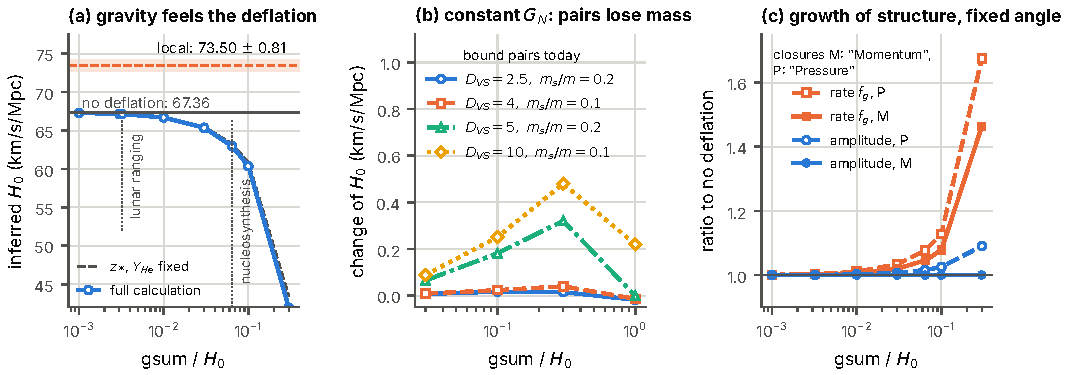
\includegraphics[width=\textwidth]{fig_hubble}
\caption{\label{fig:hubble}The Hubble constant and the growth of structure on a deflating spacetime.
(a) The Hubble constant inferred from the angular scale of the sound horizon against the rate of
deflation, if gravity feels the deflation (A1, A2): with recombination computed on the deflating
background, and with last scattering and the helium fraction held fixed; the bounds of
Table~\ref{tab:bounds} and the local measurement are marked. (b) The change of the inferred Hubble
constant if Newton's constant is held fixed and bound pairs lose rest mass. (c) Amplitude and rate of
the growth of structure relative to the model without deflation, at a fixed angle of the sound
horizon, for the two closures of Sec.~\ref{sec:pert}.}
\end{figure*}

\subsection{How fast can the coordinates deflate today?}

\begin{table*}
\caption{\label{tab:bounds}Upper bounds on the present total rate of deflation, each under the
assumption named. Uncertainties of the measured values are at 68 per cent unless stated; the bounds
are at two standard deviations. The bound in units of $H_0$ uses $H_0=67.36~\kmsMpc$. A2: gravity is
the Einstein theory in eight dimensions. HV: the vacuum value of the Vorton-Scalar sets the
electroweak scale. H2: the superfluid state is the Higgs field; the bound is given for $\nEW=1$ and
scales as $1/\nEW$ (Sec.~\ref{sec:higgs}).}
\begin{ruledtabular}
\begin{tabular}{p{0.17\textwidth}p{0.27\textwidth}p{0.15\textwidth}cc}
observation & measured & assumption & bound on $\gsum$ (per year) & in units of $H_0$ \\
\hline
lunar laser ranging \cite{HofmannMueller2018} & $(d\GN/dt)/\GN=(7.1\pm7.6)\times10^{-14}$ per year & A2 & $2.230\times10^{-13}$ & $3.237\times10^{-3}$ \\
nucleosynthesis, Newton's constant \cite{Alvey2020} & $\GN$ then, divided by $\GN$ today: $0.99^{+0.06}_{-0.05}$ (two standard deviations) & A2; constant rate & $4.434\times10^{-12}$ & 0.0644 \\
nucleosynthesis, Fermi constant \cite{ScherrerSpergel1993} & $G_{\mathrm{Fermi}}$ at $t=1$~s within 20 (10) per cent of today's value, at fixed fermion masses & HV; constant rate & $1.615\times10^{-11}$ ($7.627\times10^{-12}$) & 0.234 (0.111) \\
atomic clocks, mass ratio \cite{Lange2021} & $(d/dt)\ln(m_p/m_e)=(-8\pm36)\times10^{-18}$ per year & H2, $\nEW=1$ & $8.000\times10^{-17}$ & $1.161\times10^{-6}$ \\
atomic clocks, fine-structure constant \cite{Lange2021} & $(d\alpha_{\mathrm{em}}/dt)/\alpha_{\mathrm{em}}=(1.0\pm1.1)\times10^{-18}$ per year & an electromagnetic field along $x5,x6,x7$ (not part of the model) & $3.200\times10^{-18}$ & $4.645\times10^{-8}$ \\
\end{tabular}
\end{ruledtabular}
\end{table*}

Table~\ref{tab:bounds} and Fig.~\ref{fig:bounds} collect the bounds.

\emph{Under A2, lunar laser ranging} measures $(d\GN/dt)/\GN$ directly, and Eq.~(\ref{eq:GN}) turns
its limit into $\gsum<2.23\times10^{-13}$ per year, that is, $3.24\times10^{-3}\,H_0$. At this rate
the deflation clock has advanced by $\gsum\,t_0=3.1\times10^{-3}$ over the age $t_0$ of the universe,
and the inferred Hubble constant is lower by $0.21~\kmsMpc$.

\emph{Under A2, nucleosynthesis} bounds the ratio of Newton's constant then to its value today; for
a rate that was constant since, $\gsum<0.064\,H_0$. This is weaker than the first bound but does not
assume that the rate today equals the rate in the past.

\emph{Under HV, nucleosynthesis} bounds the change of the Fermi constant at fixed fermion masses to
10 to 20 per cent, which gives $\gsum<0.111$ to $0.234\,H_0$. HV is the assumption that the
Vorton-Scalar itself plays the role of the Higgs field, so that
$G_{\mathrm{Fermi}}=1/(\sqrt2\,\vVS^{2})$ grows as $e^{\td}$ while every mass stays constant. It is
\emph{not} the hypothesis H2, and the Vorton-Scalar, which is a singlet of every non-Abelian
symmetry of the model, cannot be the Higgs field of the Standard Model, which is a doublet; the bound
is given only to show what the assumption would imply.

\emph{Under the hypothesis H2, atomic clocks} give by far the strongest bound, and one that needs no
assumption about gravity. Section~\ref{sec:higgs} derives it: $\gsum<1.16\times10^{-6}\,H_0/\nEW$
with an exponent $\nEW$ of order one or larger.

\emph{The fine-structure constant} is bounded by the same clocks to parts in $10^{18}$ per year.
This would bound the rate, to $4.6\times10^{-8}\,H_0$, only if an electromagnetic field propagated
along the deflating coordinates. The model contains no electromagnetic field; the row shows how
strongly such an extension would be constrained.

\emph{Under A2, the microwave background} would bound the rate as well. Section~\ref{sec:forecast}
finds, as a forecast for mock data of the quality of the Planck satellite and not as a measurement,
$\gsum<0.0385\,H_0$; Fig.~\ref{fig:bounds} includes it for comparison.

\emph{In the model as it stands}, without H2, HV or an electromagnetic extension and without A2, no
mass and no coupling of ordinary matter depends on the deflation, and none of these observations
bounds the rate.

The consequence for the histories of Secs.~\ref{sec:gap} to \ref{sec:cjt} is severe. Under A2 the
clock has advanced by at most 0.0031 during the whole of cosmic history, if the rate was constant;
under H2 by at most $1.1\times10^{-6}/\nEW$. A history in which pairs become bound, matter loses its
fermion mass or the gap grows by orders of magnitude within the age of the universe requires that
gravity does not feel the deflation, that the superfluid is not the Higgs field, or that the rate
was much larger in the past than it is today.

\begin{figure*}
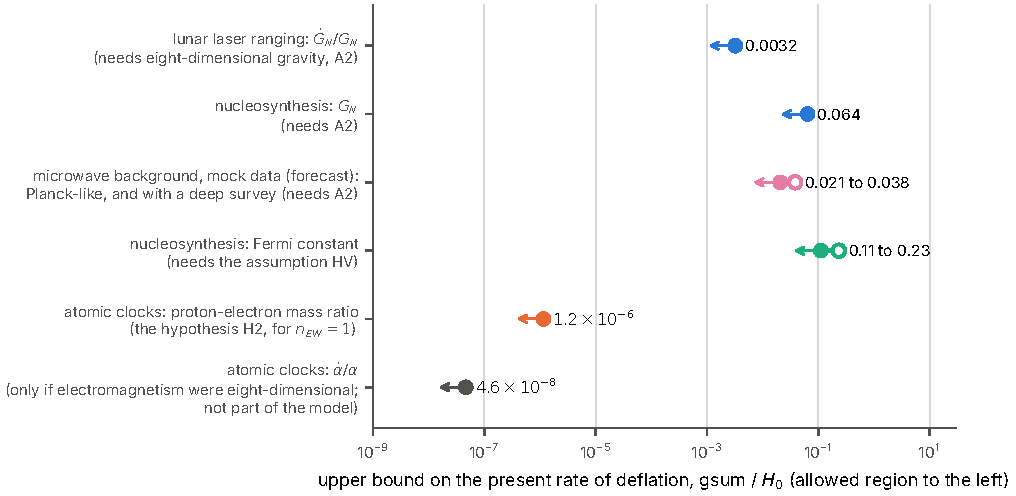
\includegraphics[width=0.8\textwidth]{fig_bounds}
\caption{\label{fig:bounds}Upper bounds on the present total rate of deflation in units of the
Hubble constant, each under the assumption of Table~\ref{tab:bounds}. The allowed region is to the
left of each bound. The row ``microwave background'' is not a measurement but the forecast of
Sec.~\ref{sec:forecast} for mock data (open symbol: Planck-like; filled symbol: with a deep
survey).}
\end{figure*}

\subsection{Bound pairs lose rest mass}

If the dark matter consists of bound pairs of the fermions, its particles have the rest mass $2m$
minus the binding energy. The binding energy grows with the coupling, so that the pairs become
lighter as the deflation proceeds, and the density of dark matter falls slightly faster than the
inverse volume. A dark matter that was heavier in the past raises the inferred Hubble constant. The
program computes the effect for four examples with $\aVS$ between 0.4 and 1 today, where the binding
energy is at most 8.2 per cent of the rest mass [Fig.~\ref{fig:hubble}(b), Table~\ref{tab:xmassloss}]. If gravity feels the
deflation, the inferred Hubble constant changes by between $-4.11$ and $-0.19~\kmsMpc$ at the rates
that nucleosynthesis and lunar laser ranging allow: the weaker gravity of the past outweighs the
loss of mass. (These examples hold $z_*$ and $\YHe$ fixed, which by Table~\ref{tab:hubble}
underestimates a fall by about six per cent of itself.) If Newton's constant is held fixed and the deflation acts on the dark sector alone,
rates between 0.03 and $1\,H_0$ raise the inferred Hubble constant by at most $+0.48~\kmsMpc$, for a
loss of up to 7.7 per cent of the rest mass. This is the only effect of the deflation found here
that raises the inferred Hubble constant, and in these examples it supplies less than a tenth of the
$6.1~\kmsMpc$ that separate the model from the local measurement.

\subsection{Perturbations of ordinary space: what must be assumed}
\label{sec:pert}

The quantities of the preceding subsections belong to the unperturbed universe. The growth of
structure and the spectra of the microwave background are built from small perturbations of
ordinary space, and the equations of the perturbations contain more of Einstein's equations than
Eq.~(\ref{eq:friedmann}). They therefore contain what the hypothesis of deflation leaves open.

\emph{The agent.} Something must keep the three rates constant while ordinary space expands and
matter dilutes. We call it the agent and assume nothing about its nature. Assumption A2 says that it
has no energy density: otherwise its density would stand on the right of Eq.~(\ref{eq:friedmann}).
It cannot be without stresses. The components of Einstein's equations along ordinary space, together
with the conservation of matter in ordinary space and Eq.~(\ref{eq:GN}), require the agent to have,
in ordinary space, the pressure
\begin{equation}
\begin{aligned}
8\pi\GN\,p_{\mathrm{agent}}={}&-\frac{\gsum}{H}\frac{dH}{dx4}-2\,\gsum\,H\\
&+2\,\gprod-\frac{\gsum\,\gprod}{3H}.
\end{aligned}
\label{eq:pagent}
\end{equation}
In an era of matter this is $-\gsum\,H/2$ to the first order in the rates. The agent is a medium
without energy density and with a tension, of the relative size $\gsum/H$. When ordinary space is
perturbed, such a medium will in general be perturbed too.

\emph{A3: the perturbations.} We assume (i) that in a universe with small inhomogeneities the scale
factors $b_t$ of the deflating coordinates remain the prescribed functions of the time, the time
being the proper time of observers who move with the cold matter, and that $x0$ remains static; and
(ii) that the agent has no energy density in the perturbed universe either. Part (i) is the plainest
reading of the hypothesis of deflation in a universe that is not exactly homogeneous; part (ii) is
A2 taken to first order. Both are assumptions.

\emph{The equations.} We use the conformal time $\tcf$ of ordinary space, defined by
$d\tcf=dx4/a_{\mathrm{sp}}$, write a prime for the derivative with respect to it, and write
$\Hcf=a_{\mathrm{sp}}'/a_{\mathrm{sp}}=a_{\mathrm{sp}}H$ for the conformal Hubble rate. A scalar
perturbation of ordinary space with the comoving wavenumber $k$ is described, in the synchronous
gauge, by two functions $\hsy(\tcf)$ and $\etasy(\tcf)$ of the perturbed metric; they are the $h$
and $\eta$ of Ref.~\cite{MaBertschinger1995}, written here with an index because $h$ and $\eta$ have
other meanings in this paper. The combination
$\alsy=(\hsy'+6\,\etasy')/2k^{2}$ occurs repeatedly. Matter and radiation enter through four sums
over the species, each multiplied by $8\pi\GN(x4)\,a_{\mathrm{sp}}^{2}$ with the Newton's constant of
the moment: $\cD$, the perturbation of the energy density; $\cT$, the divergence of the momentum
density; $\cP$, the perturbation of the pressure; and $\cA$, the anisotropic stress. With the scale
factors of the extra coordinates unperturbed, the Einstein tensor of the eight-dimensional metric
gives, to first order,
\begin{subequations}
\label{eq:pert}
\begin{align}
2k^{2}\etasy-\He\,\hsy'&=-\cD,\label{eq:E}\\
2k^{2}\etasy'&=\cT,\label{eq:M}\\
\hsy''+2\He\,\hsy'-2k^{2}\etasy&=-3\,\cP,\label{eq:T}\\
\alsy'+2\He\,\alsy-\etasy&=-\tfrac32\,\cA/k^{2},\label{eq:S}
\end{align}
\end{subequations}
with
\begin{equation}
\He=\Hcf-\tfrac12\,a_{\mathrm{sp}}\,\gsum .
\label{eq:He}
\end{equation}
They are the energy constraint, the momentum constraint, the trace of the space-space equations and
their traceless part, the equation of the shear. An independent program derives them by computer
algebra for arbitrary rates and for both signatures (Appendix~\ref{app:checks}). They are the four
equations of general relativity \cite{MaBertschinger1995} with two changes: Newton's constant is
that of the moment, and $\Hcf$ is replaced by $\He$ in three of them. The second change can be read
off Eq.~(\ref{eq:friedmann}). The time component of the Einstein tensor is the sum of the products
of all pairs of expansion rates. If the rate of one ordinary direction is perturbed, the
perturbation multiplies the sum of the rates of all \emph{other} directions, which is $2H$ in four
dimensions and $2H-\gsum$ here.

\emph{The four equations cannot all hold with matter alone.} In general relativity two of the four
equations (\ref{eq:pert}) imply the other two, because the energy and the momentum of matter are
conserved. Here they do not. Let Eq.~(\ref{eq:E}) hold, and define three \emph{gaps}, the amounts by
which the other three fail when only matter and radiation stand on their right-hand sides:
\begin{equation}
\begin{aligned}
\cYM&=2k^{2}\etasy'-\cT,\\
\cYT&=\hsy''+2\He\,\hsy'-2k^{2}\etasy+3\,\cP,\\
\cYS&=\alsy'+2\He\,\alsy-\etasy+\tfrac32\,\cA/k^{2}.
\end{aligned}
\label{eq:gaps}
\end{equation}
The conservation of the energy and of the momentum of matter in ordinary space gives two identities
between them,
\begin{align}
\cYM&=\He\,\cYT+\cZ,\label{eq:id1}\\
2k^{2}\,\cYS&=\cYT+\frac{3}{k^{2}}\big(\cYM'+2\He\,\cYM\big),\label{eq:id2}
\end{align}
with
\begin{equation}
\begin{aligned}
\cZ&=\hsy'\,\cB-\tfrac12\,a_{\mathrm{sp}}\,\gsum\,(\cD-3\,\cP),\\
\cB&=\He'-\He^{2}+\tfrac12(\cE+\cE_P).
\end{aligned}
\label{eq:Z}
\end{equation}
Here $\cE$ and $\cE_P$ are $8\pi\GN a_{\mathrm{sp}}^{2}$ times the density and the pressure of the
unperturbed universe. By Eq.~(\ref{eq:friedmann}) the quantity $\cB$ is proportional to $\gsum$; in
an era of matter it is $a_{\mathrm{sp}}\,\gsum\,\Hcf/4$. Without deflation $\cB$ and $\cZ$ vanish,
and Eqs.~(\ref{eq:id1}) and (\ref{eq:id2}) say that if one gap vanishes at all times, all three do:
that is general relativity. With deflation $\cZ\neq0$, and \emph{the three gaps cannot all vanish}.
This is not a defect of the calculation. It is the statement that the agent, which has a tension,
takes part in the perturbations: the gaps are, up to the factor $8\pi\GN a_{\mathrm{sp}}^{2}$, the
perturbations of its momentum density, of its pressure and of its anisotropic stress.

\emph{Closures.} The two identities relate three gaps; one more relation closes the system, and the
hypothesis offers no ground for a choice. Three natural choices set one gap to zero. In the closure
``Momentum'', $\cYM=0$: the agent carries no momentum density, and
Eqs.~(\ref{eq:E}) and (\ref{eq:M}) hold. In the closure ``Pressure'', $\cYT=0$: the agent carries no
perturbation of its pressure, Eqs.~(\ref{eq:E}) and (\ref{eq:T}) hold, and Eq.~(\ref{eq:M}) is
replaced by $2k^{2}\etasy'=\cT+\cZ$. In the closure ``Shear'', $\cYS=0$: the agent carries no
anisotropic stress, as a perfect fluid or a scalar field would not. Eliminating $\cYT$ from the two
identities then gives an equation of motion for the momentum density of the agent,
\begin{equation}
\cYM'=-\Big(\frac{k^{2}}{3\He}+2\He\Big)\cYM+\frac{k^{2}}{3\He}\,\cZ .
\label{eq:shearclosure}
\end{equation}
Far inside the horizon, $k\gg\Hcf$, the rate $k^{2}/3\He$ is enormous, and $\cYM$ relaxes at once to
$\cZ$, its value in the closure ``Pressure''. \emph{Inside the horizon the closure ``Shear'' is the
closure ``Pressure''}, with corrections of the relative order $(\Hcf/k)^{2}$. We compute with the
closures ``Momentum'' and ``Pressure'' and mark every result as depending on the closure or not.

All gaps are proportional to $a_{\mathrm{sp}}\,\gsum/\Hcf=\gsum/H$. At the largest rate that
nucleosynthesis allows this ratio is $2.7\times10^{-6}$ at recombination and $6.9\times10^{-2}$
today. The closure therefore cannot matter for anything that is decided at recombination, and it
must matter for the gravitational potentials and for the growth of structure of the recent universe.

\subsection{The growth of structure}

For pressureless matter with the density contrast $\delta_m$ and the density $\rho_m$ each closure
gives one equation. In the closure ``Pressure'', Eqs.~(\ref{eq:E}) and (\ref{eq:T}) give
\begin{equation}
\frac{d^{2}\delta_m}{dx4^{2}}+\Big(2H-\frac{\gsum}{2}\Big)\frac{d\delta_m}{dx4}=4\pi\,\GN(x4)\,\rho_m\,\delta_m :
\label{eq:growthP}
\end{equation}
gravity is that of the moment, and the Hubble friction is reduced by $\gsum/2$. In the closure
``Momentum'', the derivative of Eq.~(\ref{eq:E}) with Eq.~(\ref{eq:M}) gives, in conformal time,
\begin{equation}
\delta_m''+\frac{2\He'+\cE_m+\tfrac43\cE_r}{2\He}\,\delta_m'=\frac{\Hcf-a_{\mathrm{sp}}\,\gsum}{2\He}\,\cE_m\,\delta_m ,
\label{eq:growthM}
\end{equation}
where $\cE_m$ and $\cE_r$ are the parts of $\cE$ from matter and from radiation. Here the source is
reduced as well, by the factor $(H-\gsum)/(H-\gsum/2)$. (The term with $\cE_r$ is the momentum
density of radiation that streams freely: far inside the horizon its velocity divergence is
$-\hsy'/2$ \cite{MaBertschinger1995}.) Without deflation both equations reduce to the familiar
$d^{2}\delta_m/dx4^{2}+2H\,d\delta_m/dx4=4\pi\GN\rho_m\delta_m$. With deflation that familiar
equation, with $\GN(x4)$ inserted, is neither of the two. For matter alone and three equal rates the
growth rate $d\ln\delta_m/d\ln a_{\mathrm{sp}}$ is, to the first order in $\gsum/H$,
$1-\tfrac{9}{16}\,\gsum/H$ in the closure ``Pressure'' and $1-\tfrac{13}{16}\,\gsum/H$ in the closure
``Momentum''.

Two effects oppose each other [Fig.~\ref{fig:hubble}(c), Table~\ref{tab:xgrowth}]. At a \emph{fixed} Hubble constant, weaker
gravity in the past lowers the amplitude $\sigma_8$ of clustering today:
$d\ln\sigma_8/d(\gsum/H_0)=-0.443$ in the closure ``Momentum'' and $-0.207$ in the closure
``Pressure''. But the Hubble constant that keeps the angle of the sound horizon is lower, the
cosmological term takes over later, and matter clusters for longer. With that Hubble constant the net
change is $+0.003$ and $+0.239$ per unit of $\gsum/H_0$: $+0.001$ and $+0.077$ per cent at the bound
of lunar laser ranging, and $+0.01$ and $+1.60$ per cent at the bound of nucleosynthesis. The growth
rate today, $f_g=d\ln\delta_m/d\ln a_{\mathrm{sp}}$, rises in both closures, by the factors 1.0021
and 1.0035 at the first bound and 1.0463 and 1.0773 at the second. Common to both closures is that,
at a fixed angle, the amplitude does not fall and the growth rate rises. How large the changes are
depends on the closure: \emph{the growth of structure on the deflating spacetime is not predicted
until the perturbations of the agent are specified.}

\subsection{The spectra of the microwave background}
\label{sec:spectra}

\emph{The program.} The temperature and polarization spectra of the microwave background and the
power spectrum of matter are computed with an Einstein-Boltzmann program written for this work. It
integrates the equations of motion of photons, neutrinos, baryons and cold dark matter in the
synchronous gauge \cite{MaBertschinger1995} together with the equations of the metric perturbations,
and obtains the spectra by integrating the sources along the line of sight
\cite{SeljakZaldarriaga1996}. Its version for static extra coordinates has Newton's constant built
into its units. For the deflating spacetime four of its parts were copied and changed in a short,
listed set of places: the
expansion obeys Eq.~(\ref{eq:friedmann}); every source of the metric perturbations carries the
Newton's constant of the moment; the energy constraint is Eq.~(\ref{eq:E}); and the sources of the
temperature anisotropy contain the gap $\cYS$ of the closure. The equations of motion of photons,
neutrinos, baryons and dark matter are not changed: matter that is spread uniformly over the extra
coordinates moves in ordinary space as it does in four dimensions, and Thomson scattering and
recombination are atomic physics, which the model does not alter. The copies are written by a script
from the original files, so that they cannot differ from them in any place that is not listed, and
without deflation the two versions give the same spectra to the last binary digit.

\emph{Recombination and helium.} Recombination is computed on the expansion history of
Eq.~(\ref{eq:friedmann}), with the three-level atom and its standard corrections
\cite{SeagerSasselovScott1999}. The helium fraction responds as well. At nucleosynthesis Newton's
constant was smaller than today by the factor $\GN$ ratio of Table~\ref{tab:hubble}; a universe that
expands more slowly by that factor in $H^{2}$ is equivalent, for nucleosynthesis, to one with
$\tfrac{43}{7}(\GN\ \text{ratio}-1)$ additional neutrino species, a negative number, and the helium
fraction follows from the standard fit \cite{Planck2015XIII}. (In a model with extra radiation,
$\tfrac{43}{7}$ is replaced by $\tfrac{43}{7}+\Delta N$, where $\Delta N$ is the density of that
radiation during nucleosynthesis in units of one neutrino species.) At the largest rate that
nucleosynthesis allows, and without extra radiation, this is $-0.379$ species, and $\YHe$ falls
from 0.24540 to 0.24008. Table~\ref{tab:xbackground} gives the thermal history of three models.

\emph{Spectra at a fixed angle.} Table~\ref{tab:spectra} lists the model without deflation and
five models with three equal rates, each with the densities, the primordial amplitude and tilt and the optical depth of the standard
model and with the Hubble constant that keeps $100\,\theta_*=1.03965$. Keeping the angle keeps the
acoustic peaks in place: the first five move by at most 0.32 in the multipole $\ell$
(Table~\ref{tab:xpeaks}). What changes is
their height and the damping tail [Fig.~\ref{fig:spectra}], for the reasons that apply to any change
of the expansion rate at recombination: the ratio of the diffusion length to the sound horizon, the
width of the last-scattering surface and the decay of the potentials shortly after recombination all
change, and the lower helium fraction leaves more electrons per baryon.

\begin{table*}
\caption{\label{tab:spectra}Spectra of the microwave background on the deflating spacetime at a fixed
angle of the sound horizon (assumptions A1, A2, A3; three equal rates). $H_0$ in $\kmsMpc$.
$\GN(z_*)/\GN$: Newton's constant at last scattering divided by its value today. $\sigma_8$:
amplitude of clustering for the same primordial amplitude, in the closures ``Momentum'' (M) and
``Pressure'' (P). Largest change: of the temperature spectrum $D_\ell^{TT}$ for $30\le\ell\le2500$
relative to the model without deflation. Ideal measurement: the root of the sum over those
multipoles of the squared change divided by the variance $2/(2\ell+1)$ of one multipole, that is,
the number of standard deviations by which a measurement of the temperature on the whole sky without
noise would tell the model from no deflation if nothing else were unknown. $\Delta\chi^{2}$: against
Planck-like mock data with all other parameters fixed.}
\begin{ruledtabular}
\begin{tabular}{cccccccc}
$\gsum/H_0$ & $H_0$ & $\GN(z_*)/\GN$ & $\sigma_8$ (M) & $\sigma_8$ (P) & largest change & ideal measurement & $\Delta\chi^{2}$ \\
\hline
0 & 67.360 & 1.0000 & 0.8228 & 0.8228 & 0 & 0.0 & 0.00 \\
0.00324 & 67.149 & 0.9969 & 0.8219 & 0.8225 & $2.7\times10^{-3}$ & 3.1 & 1.12 \\
0.0100 & 66.704 & 0.9905 & 0.8200 & 0.8219 & $8.3\times10^{-3}$ & 9.7 & 10.79 \\
0.0300 & 65.365 & 0.9714 & 0.8142 & 0.8201 & 0.025 & 29.5 & 98.85 \\
0.0644 & 62.976 & 0.9383 & 0.8032 & 0.8160 & 0.056 & 64.8 & 468.30 \\
0.100 & 60.368 & 0.9037 & 0.7903 & 0.8104 & 0.090 & 103.5 & 1166.70 \\
\end{tabular}
\end{ruledtabular}
\end{table*}

At the rate that lunar laser ranging allows, the temperature spectrum differs from that of the
model without deflation by at most $2.7\times10^{-3}$ of itself, 0.134 of the cosmic variance of a
single multipole, and $\Delta\chi^{2}=1.12$ against Planck-like mock data
(Sec.~\ref{sec:forecast}) before any parameter is refitted. Such data cannot tell this rate from no
deflation. At the rate that nucleosynthesis allows, Newton's constant at last scattering was 0.9383
of today's, the spectrum changes by up to 5.6 per cent, and $\Delta\chi^{2}=468$: the microwave
background is then a stronger test than nucleosynthesis.

\begin{figure*}
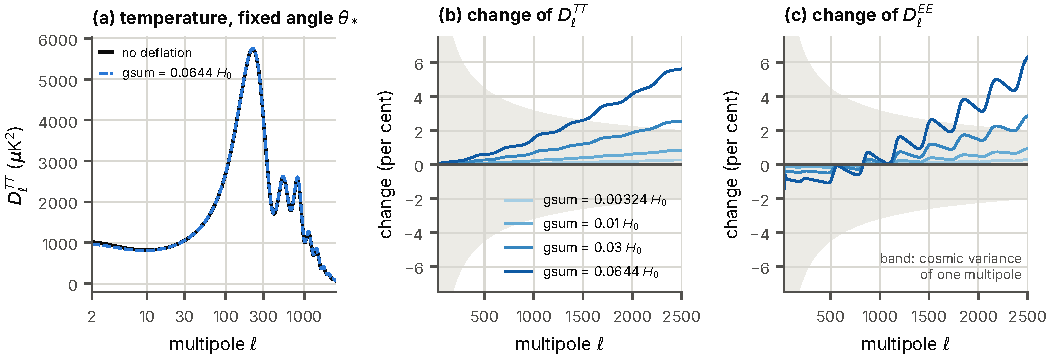
\includegraphics[width=\textwidth]{fig_spectra}
\caption{\label{fig:spectra}The spectra of the microwave background at a fixed angle of the sound
horizon. (a) The temperature spectrum without deflation and at the largest rate that nucleosynthesis
allows. (b), (c) The change of the temperature and polarization spectra relative to the model
without deflation for four rates (darker: faster); the band is the cosmic variance of a single
multipole. Closure ``Momentum''; at these multipoles the closure ``Pressure'' gives the same
curves.}
\end{figure*}

\emph{The closure.} For $30\le\ell\le2500$ the spectra of the two closures differ by a thousandth of
the effect of the deflation itself ($1.4\times10^{-3}$ and $1.2\times10^{-3}$ of it at the two
bounds), and $\Delta\chi^{2}$ is the same to five digits [Fig.~\ref{fig:closure}(a)]. \emph{The
spectra at these multipoles follow from A1, A2 and A3, whatever the closure.} For
$\ell<30$, where the potentials of the recent universe act through the late integrated Sachs-Wolfe
effect, the closures differ by more than the effect of the deflation in either of them, by a factor
2.1. The largest angular scales are not predicted; their cosmic variance is large, and at the rate
of nucleosynthesis the closures differ by at most a third of it. The amplitude of matter is 0.9762
of its value without deflation in the closure ``Momentum'' and 0.9918 in the closure ``Pressure'' at
the rate of nucleosynthesis, and 0.99892 and 0.99969 at the rate of lunar laser ranging
(Table~\ref{tab:xclosure}).

Figure~\ref{fig:closure}(b) and Table~\ref{tab:xgaps} show what the agent must supply. In units of $a_{\mathrm{sp}}\,\gsum/\Hcf$
times the terms of each equation, the closure ``Momentum'' lacks 0.54 to 0.98 in Eq.~(\ref{eq:T}) and
0.31 to 0.49 in Eq.~(\ref{eq:S}) after recombination; the closure ``Pressure'' lacks 0.62 to 0.94 in
Eq.~(\ref{eq:M}), and in Eq.~(\ref{eq:S}) an amount that falls as $(\Hcf/k)^{2}$ inside the horizon,
as Eq.~(\ref{eq:shearclosure}) requires. The two identities (\ref{eq:id1}) and (\ref{eq:id2}) hold
along the numerical solutions to $8.6\times10^{-4}$, the accuracy of the numerical derivative with
which they are tested. The complete calculation, with photons, neutrinos and baryons, reproduces the
growth of Eqs.~(\ref{eq:growthP}) and (\ref{eq:growthM}) to $1.3\times10^{-4}$
[Fig.~\ref{fig:closure}(c), Tables~\ref{tab:xebgrowth} and \ref{tab:xebgrowth2}]; with the
equation of the other closure it would disagree by a quarter of $\gsum/H_0$.

\begin{figure*}
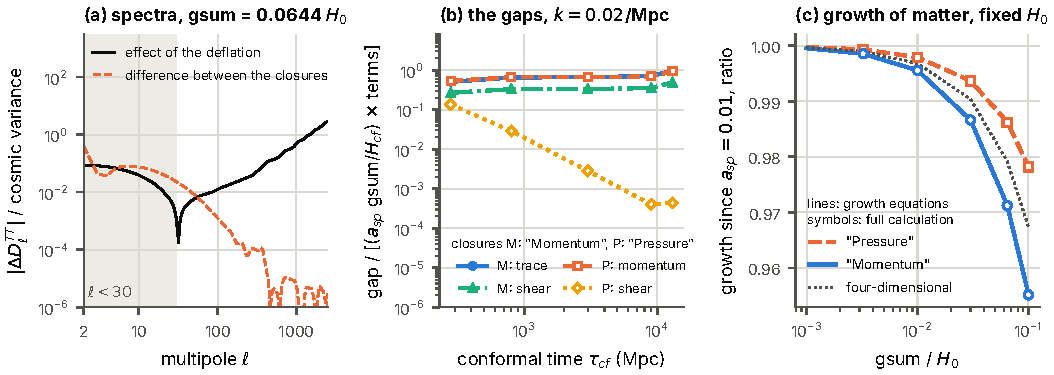
\includegraphics[width=\textwidth]{fig_closure}
\caption{\label{fig:closure}The closure of the perturbation equations, at the largest rate that
nucleosynthesis allows. (a) The difference between the temperature spectra of the closures
``Momentum'' and ``Pressure'', and the effect of the deflation itself, in units of the cosmic
variance of a single multipole: the closure matters below $\ell=30$ only. (b) What the agent
supplies: the gaps of Eqs.~(\ref{eq:M}), (\ref{eq:T}) and (\ref{eq:S}) for one wavenumber, in units
of $a_{\mathrm{sp}}\,\gsum/\Hcf$ times the terms of each equation. (c) The growth of the density
contrast of matter since $a_{\mathrm{sp}}=0.01$ relative to no deflation, at a fixed Hubble constant:
Eqs.~(\ref{eq:growthP}) and (\ref{eq:growthM}) (lines), the complete calculation (symbols), and the
four-dimensional equation with the Newton's constant of the moment, which is neither closure.}
\end{figure*}

\subsection{What mock data say about the rate, and about the Hubble constant}
\label{sec:forecast}

How far can the rate of deflation move the Hubble constant before the fit to the microwave
background degrades? The question is answered here with mock data: the spectra of the standard model
stand in for the measurements, with the noise and the sky coverage of the Planck satellite
\cite{Planck2015XIII}, and of Planck together with a deep survey of a quarter of the sky. The mock
data contain no gravitational lensing, and the standard model fits them with $\Delta\chi^{2}=0$ by
construction. The likelihood is the Gaussian likelihood of the temperature and polarization spectra
with these noise levels; the six parameters of the standard model (the densities $\omega_b$ and
$\omega_c$, the Hubble constant, the amplitude $A_s$ and the spectral index $n_s$ of the primordial
fluctuations, and the optical depth $\tau$) are fitted again for every rate; the rate is a seventh
parameter. Because the rates are positive, the derivative of the spectra with respect to $\gsum$ at
zero rate is one-sided.

\begin{table*}
\caption{\label{tab:fisher}Forecast for the rate of deflation from mock data of the microwave
background (Fisher matrix; three equal rates; assumptions A1, A2, A3). M, P: the closures
``Momentum'' and ``Pressure''. $\sigma_{\mathrm{rate}}$:
standard error of $\gsum/H_0$ with the six parameters of the standard model free. Bound: the upper
bound at 95 per cent, 1.96 standard errors, for a parameter that cannot be negative and whose best
value is zero. Held: the standard error if the six parameters are held fixed. Slope: the change of the
best-fit Hubble constant per unit of $\gsum/H_0$, in $\kmsMpc$. Last two columns: the standard error
of the Hubble constant in $\kmsMpc$ with the rate held at zero, and with the rate free.}
\begin{ruledtabular}
\begin{tabular}{llcccccc}
mock data & closure & $\sigma_{\mathrm{rate}}$ & bound & held & slope & error of $H_0$ & rate free \\
\hline
Planck-like & M & 0.01963 & 0.0385 & 0.00108 & $-84.35$ & 0.561 & 1.748 \\
Planck-like & P & 0.01974 & 0.0387 & 0.00108 & $-84.40$ & 0.561 & 1.758 \\
with deep survey & M & 0.01056 & 0.0207 & 0.00055 & $-82.11$ & 0.372 & 0.943 \\
with deep survey & P & 0.01058 & 0.0207 & 0.00055 & $-82.13$ & 0.372 & 0.945 \\
\end{tabular}
\end{ruledtabular}
\end{table*}

\emph{A bound, as a forecast.} With the six parameters free, Planck-like data determine $\gsum/H_0$
to 0.0196 (Table~\ref{tab:fisher}), and the upper bound at 95 per cent is
\begin{equation}
\gsum<0.0385\,H_0=2.65\times10^{-12}\ \text{per year},
\end{equation}
or $0.0207\,H_0$ with the deep survey. With the six parameters \emph{held} the error would be
0.00108: nearly all of the effect of the deflation on the spectra, above all the shift of the angle
$\theta_*$, can be absorbed by the other parameters [Fig.~\ref{fig:forecast}(c)]. The bound lies
between those of Table~\ref{tab:bounds}: it is 11.9 times weaker than that of lunar laser ranging and
1.7 times stronger than that of nucleosynthesis. The closure changes it by half a per cent.

\emph{The Hubble constant falls in every fit.} Along the degeneracy the best-fit Hubble constant
changes by $-84.35~\kmsMpc$ per unit of $\gsum/H_0$ for the Planck-like data and by $-82.11$ with the
deep survey, that is, by $-3.2$ and $-1.7~\kmsMpc$ at the respective bounds. This is steeper than the
slope $-65.24$ at a fixed angle and fixed densities, because in the fit the density of dark matter
rises and the tilt falls as well. Fits of the six parameters at fixed rates confirm the Fisher
matrix [Fig.~\ref{fig:forecast}(a), (b); Table~\ref{tab:xfcprofile}]: for rates up to $0.01\,H_0$ the minimum $\Delta\chi^{2}$ and
the shift of the Hubble constant are 1.00 to 1.01 times its predictions, and the fits reach
$\Delta\chi^{2}=3.84$ at $\gsum=0.0376\,H_0$ and, with the deep survey, at $0.0205\,H_0$. At the rate
that lunar laser ranging allows the best fit has $\Delta\chi^{2}=0.027$ and $H_0=67.086~\kmsMpc$. At
the rate that nucleosynthesis allows it has $\Delta\chi^{2}=11.6$, a deviation of 3.4 standard
deviations, and $H_0=61.70~\kmsMpc$; with the deep survey $\Delta\chi^{2}=39.8$. \emph{The largest
rate that nucleosynthesis allows would be excluded by data of the quality of Planck.}

\begin{figure*}
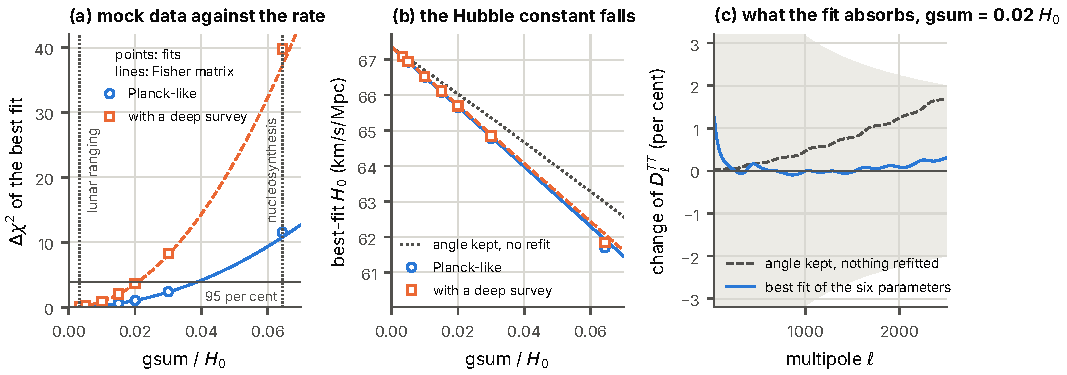
\includegraphics[width=\textwidth]{fig_forecast}
\caption{\label{fig:forecast}Mock data of the microwave background against the rate of deflation.
(a) The minimum $\Delta\chi^{2}$ of fits of the six parameters of the standard model at a fixed rate
(symbols) and the parabola of the Fisher matrix (lines), for the two data sets; the rates that lunar
laser ranging and nucleosynthesis allow are marked, and the horizontal line is $\Delta\chi^{2}=3.84$,
the bound at 95 per cent. (b) The best-fit Hubble constant, with the slope
of the Fisher matrix and, dotted, the Hubble constant that keeps the angle when nothing else is
refitted. (c) The temperature spectrum at $\gsum=0.02\,H_0$ relative to the data: with the angle kept
and nothing refitted, and at the best fit, which absorbs most of the difference; the band is the
cosmic variance of a single multipole.}
\end{figure*}

\emph{Deflation and dark radiation together.} Extra radiation is the candidate of the model for the
Hubble tension. Seven one-parameter families of extra radiation were fitted to the same mock data,
each with a density $N$ in units of one neutrino species: radiation that streams freely; a fluid;
the \emph{stepped fluid of the model}, at four transition redshifts $z_t$; and the stepped fluid of
the Wess-Zumino model \cite{Aloni2022}. The stepped fluid of the model is the massless phase mode of
the Vorton-Scalar in equilibrium with the sixteen components of the fermion field: when the
fermions become non-relativistic, at the redshift $z_t$, they annihilate and heat the phase mode, so
that the temperature of the fluid rises by the factor $15^{1/3}$ relative to the law of dilution
($N$ is the density after this step; the Wess-Zumino fluid has the factor $(15/7)^{1/3}$). Every
family can raise the Hubble constant, and every one at a price in $\Delta\chi^{2}$. Does the
deflation lower the price? All fits were made with static extra coordinates and on the deflating
spacetime at the largest rate that lunar laser ranging allows, and the Fisher matrix was computed
with $N$ and the rate free together (Table~\ref{tab:families}, Fig.~\ref{fig:families};
Tables~\ref{tab:xfamfisher} to \ref{tab:xfamjoint} of Appendix~\ref{app:tables}). Three
results follow.

First, at that rate every best-fit Hubble constant of the static case falls by 0.274 to
$0.279~\kmsMpc$, which is the shift of the model without extra radiation: the effects of the
deflation and of the extra radiation add [Fig.~\ref{fig:families}(a), (b)].

Second, $N$ and the rate are positively correlated, with correlation coefficients of 0.37 to 0.89.
Extra radiation makes the early universe expand faster, the weaker gravity of the deflating
spacetime makes it expand more slowly, and in the spectra the two compensate in part. Fits with
extra radiation are therefore slightly \emph{better} on the deflating spacetime than on the static
one, slightly more extra radiation is allowed at a given $\Delta\chi^{2}$, and with both parameters
free the error of each grows, for free-streaming radiation from 0.143 to 0.250 in $N$.

Third, the compensation does not help the Hubble constant. When the rate grows and $N$ follows its
best-fitting value, the best-fit Hubble constant still falls: by $35.3~\kmsMpc$ per unit of
$\gsum/H_0$ for free-streaming radiation, against 84.35 without extra radiation, and by 22.1 to 76.9
for the seven families. The largest Hubble constant among the models with $N\ge0$, $\gsum\ge0$ and
$\Delta\chi^{2}\le3.84$ is therefore reached at zero rate, for every family and both data sets
[Fig.~\ref{fig:families}(c)]. \emph{The deflation lowers the Hubble constant faster than it makes
room for extra radiation.}

\begin{table*}
\caption{\label{tab:families}The seven families of dark radiation on the deflating
spacetime (Planck-like mock data; assumptions A1, A2, A3). ``Model fluid'' is the stepped fluid of
the model with the transition redshift $z_t$. Columns 2 to 5: the density $N$ of extra
radiation at which the best fit reaches $\Delta\chi^{2}=4$, and the Hubble constant there in
$\kmsMpc$, with static extra coordinates and deflating at the largest rate that
lunar laser ranging allows. Columns 6 to 10, from the Fisher matrix with $N$ and the rate free together: the standard
error of $N$ with the rate held at zero and with the rate free; the correlation coefficient of $N$
and the rate; the net slope, that is, the change of the best-fit Hubble constant in $\kmsMpc$ per
unit of $\gsum/H_0$ when $N$ follows its best-fitting value; and the largest rise of the best-fit
Hubble constant, in $\kmsMpc$, among the models with $N\ge0$, $\gsum\ge0$ and
$\Delta\chi^{2}\le3.84$, which is reached at zero rate for every family.}
\begin{ruledtabular}
\begin{tabular}{lccccccccc}
 & \multicolumn{2}{c}{$N$ at $\Delta\chi^{2}=4$} & \multicolumn{2}{c}{$H_0$ there} & \multicolumn{2}{c}{error of $N$} & & net & largest \\
family & static & deflating & static & deflating & rate zero & rate free & correlation & slope & rise \\
\hline
free-streaming radiation & 0.29 & 0.31 & 69.74 & 69.62 & 0.143 & 0.250 & 0.82 & $-35.3$ & 2.30 \\
fluid, no step & 0.27 & 0.29 & 70.20 & 70.12 & 0.135 & 0.249 & 0.84 & $-23.9$ & 2.77 \\
model fluid, $z_t=10^4$ & 0.25 & 0.26 & 68.75 & 68.53 & 0.122 & 0.145 & 0.54 & $-65.4$ & 1.35 \\
model fluid, $z_t=2\times10^4$ & 0.17 & 0.18 & 68.16 & 67.90 & 0.085 & 0.091 & 0.37 & $-76.9$ & 0.78 \\
model fluid, $z_t=5\times10^4$ & 0.12 & 0.13 & 68.48 & 68.27 & 0.060 & 0.076 & 0.61 & $-67.0$ & 1.10 \\
Wess-Zumino fluid, $z_t=2\times10^4$ & 0.32 & 0.35 & 70.13 & 70.06 & 0.160 & 0.350 & 0.89 & $-22.1$ & 2.69 \\
model fluid, $z_t=10^6$ & 0.30 & 0.32 & 70.39 & 70.32 & 0.150 & 0.250 & 0.80 & $-23.0$ & 2.95 \\
\end{tabular}
\end{ruledtabular}
\end{table*}

\begin{figure*}
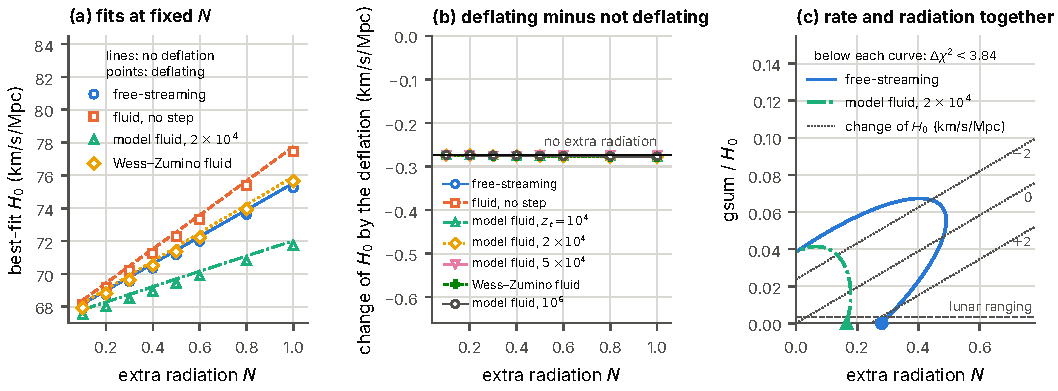
\includegraphics[width=\textwidth]{fig_families}
\caption{\label{fig:families}The seven families of dark radiation on the deflating
spacetime (Planck-like mock data). (a) The best-fit Hubble constant against the density $N$ of extra
radiation for four families: without deflation (lines) and at the largest rate that lunar laser
ranging allows (symbols). (b) The difference for all seven families; the horizontal line is the
shift of the model without extra radiation. (c) The rate and the extra radiation as free parameters
together: the regions with $\Delta\chi^{2}<3.84$ of the Fisher matrix for two families, lines of
constant change of the best-fit Hubble constant for free-streaming radiation (dotted), the point of
the largest Hubble constant of each region (filled symbols, at zero rate), and the rate that lunar
laser ranging allows (dashed).}
\end{figure*}

\subsection{Dark matter}
\label{sec:dm}

\emph{What does not change.} A superfluid needs particles that are degenerate (fermions) or
condensed (bound pairs) at the mass density $\rho$ and the velocity dispersion $\sigma_v$ of observed
halos. A gas of fermions with $\nu=8$ internal states is degenerate if its Fermi velocity is at
least $\sigma_v$, and bosons of the mass $m_B$ are condensed if the number of particles in a cube
with the edge of their thermal wavelength, at the temperature $k_BT=m_B\sigma_v^{2}$, is at least
2.612. Both conditions are upper limits on the mass,
\begin{equation}
m_{\mathrm{deg}}=\Big[\frac{6\pi^{2}\hbar^{3}\rho}{\nu\,\sigma_v^{3}}\Big]^{1/4},\qquad
m_{B,\max}=\Big[\frac{(2\pi)^{3/2}\hbar^{3}\rho}{2.612\,\sigma_v^{3}}\Big]^{1/4},
\label{eq:mdeg}
\end{equation}
the first being the bound of Tremaine and Gunn \cite{TremaineGunn1979} for this model. They contain
the densities and the velocities only, and the masses of the model do not change along the
deflation (Table~\ref{tab:halos}): in the densest systems of dark matter that are observed, the
cores of dwarf spheroidal galaxies, fermions are degenerate only if they are lighter than 0.276~keV
and bound pairs are condensed only if they are lighter than 262~eV. The first limit conflicts with
the bound of the Lyman-$\alpha$ forest derived below, which demands more than 1.5~keV; the second
conflicts with the bound on the self-interaction of the pairs, which demands far heavier fermions.
\emph{The dark matter of galaxies is not a superfluid of these particles.} Heavy fermions or pairs
can be cold dark matter of an ordinary kind. The deflation does not change this verdict.

\begin{table*}
\caption{\label{tab:halos}Could the fermions of the model be degenerate, or their bound pairs
condensed, in observed systems of dark matter? $\rho$: density; $\sigma_v$: velocity dispersion;
$m_{\mathrm{deg}}$ and $m_{B,\max}$: the limits of Eq.~(\ref{eq:mdeg}).}
\begin{ruledtabular}
\begin{tabular}{lcccc}
system & $\rho$ ($M_\odot$ pc$^{-3}$) & $\sigma_v$ (km/s) & $m_{\mathrm{deg}}$ (keV) & $m_{B,\max}$ (eV) \\
\hline
dwarf spheroidal galaxy, core & 0.100 & 10 & 0.276 & 262 \\
Milky Way at the Sun & 0.0105 & 156 & 0.020 & 19.0 \\
cluster of galaxies, core & 0.00300 & 1000 & 0.004 & 3.45 \\
\end{tabular}
\end{ruledtabular}
\end{table*}

\emph{Self-interaction, and the epoch of the resonance.} The cross-section per mass of bound pairs
must respect the bound of about $\kappa_{\mathrm{SI}}=1~\mathrm{cm^{2}/g}$ from colliding clusters
\cite{Markevitch2004,Randall2008}. A pair bound by the Yukawa potential (\ref{eq:yukawa}) has a
scattering length of at least the range $1/m_s$; identical bosons with that scattering length
scatter at low energy with the cross-section $8\pi/m_s^{2}$; and the pair exists only if
$\DVS=\aVS\,m/m_s>D_c$ (Sec.~\ref{sec:pair}). Together, for pairs of the mass $2m$, these give a
smallest fermion mass,
\begin{equation}
m\ge\Big[\frac{4\pi\,D_c^{2}}{\aVS^{2}\,\kappa_{\mathrm{SI}}}\Big]^{1/3},
\label{eq:mmin}
\end{equation}
which is 918~MeV for $\aVS=0.1$ and falls as $\aVS^{-2/3}$, that is, as $e^{-2\td/3}$ along the
deflation. For a given particle the masses are constant and so is this
cross-section. What the deflation changes is whether the pair \emph{exists}: it is bound only after
$\DVS$ has grown to $D_c$. And at that moment the scattering length of two unbound fermions
diverges (Sec.~\ref{sec:pair}), so that their cross-section rises to the limit that unitarity
allows, which is larger the slower the particles. For the example particle, $m=918$~MeV and
$m_s=54.7$~MeV, at the relative velocities 10, 156 and 1000~km/s [Fig.~\ref{fig:binding}(c)]: one
unit of the clock before the binding the cross-section per mass is $0.84~\mathrm{cm^{2}/g}$ at all
three velocities; at the binding it peaks at $1.3\times10^{7}$, $5.2\times10^{4}$ and
$1.3\times10^{3}~\mathrm{cm^{2}/g}$; and it exceeds $100~\mathrm{cm^{2}/g}$ during an interval of the
clock of 0.27, 0.27 and 0.26 around the binding. \emph{A deflating universe whose dark matter
consists of these fermions passes through an epoch of strong, velocity-dependent self-interaction},
strongest in the smallest halos. Whether the epoch lies in the observable past depends on the rate.
Under A2 and a constant rate it does so only if $\DVS$ today exceeds $D_c$ by less than a third of a
per cent, a coincidence that nothing in the model explains.

\emph{Superfluid dark matter and small-scale structure.} What becomes
of the growth of structure if the dark matter is the superfluid itself, a fluid with first sound? Two
limits are computed: a degenerate gas of the fermions with eight internal states, and a condensate of bound
pairs with the sound speed $c_{s0}$ today. The pressure of such a fluid suppresses structure below a
wavenumber, and the bound of the Lyman-$\alpha$ forest on warm dark matter
\cite{Viel2005,Irsic2017} then limits the fermion mass from below and the sound speed from above.
Computed again on the deflating background under A1 to A3, at the Hubble constant that keeps the
angle, the wavenumber at which the power falls to a quarter of that of cold dark matter is lower by
0.15 to 0.16 per cent at the rate that lunar laser ranging allows and by 3.0 to 3.3 per cent at the
rate that nucleosynthesis allows, for fifteen models (Fig.~\ref{fig:sfdm},
Tables~\ref{tab:xsfdmhalf} and \ref{tab:xsfdmbounds}). The reason is the weaker gravity of the time
at which the suppression is set: the Jeans wavenumber is proportional to the square root of Newton's
constant. The limits move accordingly, from $m>1.514$~keV and $c_{s0}<1.645\times10^{-11}\,c$ without
deflation to $m>1.516$~keV and $c_{s0}<1.641\times10^{-11}\,c$ at the first rate and $m>1.555$~keV
and $c_{s0}<1.565\times10^{-11}\,c$ at the second. The two closures give the same wavenumbers to
$1.5\times10^{-5}$. In this calculation the equation of state of the superfluid in ordinary space is
that of static extra coordinates; whether the self-interaction of a condensate would itself follow
the volume of the deflating coordinates is a question about the microscopic model that the
calculation does not answer.

\begin{figure*}
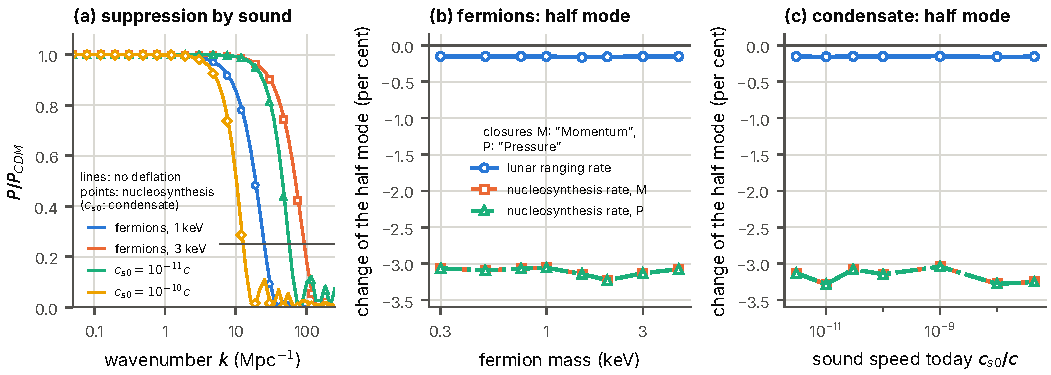
\includegraphics[width=\textwidth]{fig_sfdm}
\caption{\label{fig:sfdm}Superfluid dark matter on the deflating spacetime. (a) The power spectrum of
matter divided by that of cold dark matter, for a degenerate gas of the fermions of two masses and
for a condensate of bound pairs with two sound speeds today: without deflation (lines) and at the
rate that nucleosynthesis allows (symbols). The horizontal line marks one quarter, the value that
defines the half mode. (b) The change of the wavenumber of the half mode for the degenerate gas,
against the fermion mass, at the rates that lunar laser ranging and nucleosynthesis allow, for the
closures ``Momentum'' (M) and ``Pressure'' (P). (c) The same for the condensate, against its sound
speed today.}
\end{figure*}

\emph{How fast the quantities drift.} With $n=d\ln(\text{quantity})/d\td$, the relative change of a
quantity over the age of the universe is $n\,\gsum\,t_0$. The couplings themselves drift with $n=1$
or $\tfrac12$ (Table~\ref{tab:exponents}). Quantities near a threshold drift much faster: the
scattering length just below the binding, at $\DVS=1.5$, with $n=9.1$; the binding energy just above
it, at $\DVS=1.8$, with $n=30$; the gap of a weakly paired state with $n=1/\lambda$. These are the
quantities in which a slow deflation would first be seen (Table~\ref{tab:xdrift}).


\subsection{Verdict on hypothesis H3}

\emph{The Hubble tension.} The candidate of the model, the phase mode of the Vorton-Scalar as dark
radiation, is untouched at the allowed rates, since the couplings drift by parts in a thousand: with
static extra coordinates it raises the Hubble constant by the amounts of the last column of
Table~\ref{tab:families} at most, a fraction of the $6.1~\kmsMpc$ that are needed, and the deflation
does not improve this. The deflation itself contributes two effects. The
first, through Newton's constant, has the wrong sign: at a fixed angle of the sound horizon the
inferred Hubble constant falls by $0.2~\kmsMpc$ at the largest rate that lunar laser ranging allows,
and in fits to mock data of the microwave background it falls by $84~\kmsMpc$ per unit of
$\gsum/H_0$. Nor can the rate help the dark radiation: more extra radiation is allowed when the rate
is free, but the largest Hubble constant that the mock data allow is reached at zero rate. The
second effect, the loss of mass of bound pairs, has the right sign and is bounded, in the examples
computed, to $0.5~\kmsMpc$. \emph{The hypothesis that the model resolves the Hubble tension is not
supported by the deflation, and under A2 it is mildly disfavored.}

\emph{Dark matter.} The mass ranges stated above hold unchanged, and
the limits on superfluid dark matter move by two tenths of a per cent at the rate that lunar laser
ranging allows. The deflation adds one qualitative prediction, the epoch of the resonance, and one
quantitative one, a rise of the growth rate, whose size depends on the perturbations of the agent.
Neither is in conflict with observation at the allowed rates, and neither is detectable at the rate
that lunar laser ranging allows. \emph{The hypothesis that the superfluid is the dark matter is
neither strengthened nor weakened by the deflation.} It acquires a history, whose observable part is
empty if gravity is eight-dimensional and the rate constant.

\emph{What rests on the additional assumptions.} Everything in this section that concerns Newton's
constant rests on A2. The spectra, the forecast and the growth of structure rest in addition on A3,
and the growth of structure and the largest angular scales on a closure that the hypothesis of
deflation does not supply. The forecasts are for mock data without gravitational lensing; no
measured spectrum has been fitted.

\section{The Higgs hypothesis}
\label{sec:higgs}

\subsection{The hypothesis and the conditions}

Hypothesis H2 says that the superfluid state, the condensate of the fermion pair along the hidden
axis, \emph{is the Higgs field} \cite{Higgs1964}. In the Standard Model the Higgs field is a doublet
of the weak-isospin group with a vacuum value $\vEW=246$~GeV, which breaks the electroweak symmetry,
gives the W and Z bosons and the quarks and charged leptons their masses, and leaves one scalar
particle of 125~GeV. Its four real components form a vector of a group $SO(4)$, which the vacuum
value breaks to $SO(3)$ \cite{Sikivie1980}. From these facts follow seven conditions that
a condensate must meet in order to \emph{be} the Higgs field (Table~\ref{tab:conditions}).
With static additional times the hypothesis has no geometric basis on the $4{+}4$ spacetime,
because the condensate is a singlet under the only non-Abelian symmetry that the geometry
provides. This
section examines the conditions on the deflating spacetime.

Two statements must be kept apart. H2 is the hypothesis that the \emph{pair condensate} is the Higgs
field; the electroweak scale is then the scale of the condensate. HV, used in one row of
Table~\ref{tab:bounds}, is the different assumption that the vacuum value of the
\emph{Vorton-Scalar} sets the electroweak scale. HV is not examined here.

\begin{table*}
\caption{\label{tab:conditions}The conditions that a condensate must meet in order to be the Higgs
field, and their status on the deflating $4{+}4$ spacetime. The last row is a condition
that only a deflating spacetime imposes. A dash marks a condition that is not examined for this
spacetime, because C3 is not met there by any symmetry of the spacetime.}
\begin{ruledtabular}
\begin{tabular}{p{0.32\textwidth}p{0.62\textwidth}}
condition & status \\
\hline
C1: a scalar under the Lorentz group of ordinary spacetime & met in the sector of fields that do not depend on the extra coordinates \\
C2: non-zero in empty space & open; reached by the deflation only outside the range of validity of the model \\
C3: a doublet of the weak-isospin group with a neutral component & only under a hidden symmetry, which a contact self-interaction of form C breaks; a singlet under the rotations of the additional times \\
C4: breaks $SO(4)$ to $SO(3)$ & met in the sector only, and only without a contact self-interaction of form C \\
C5: scale 246~GeV, with a scalar particle of 125~GeV with the observed couplings & --- \\
C6: its couplings give the quarks and leptons their masses & --- \\
C7: no further light or charged particles that would have been seen & --- \\
new: the electroweak scale does not drift & requires $\gsum<1.16\times10^{-6}\,H_0/\nEW$ \\
\end{tabular}
\end{ruledtabular}
\end{table*}

\subsection{What the deflation leaves unchanged}

The pair operators, their transformation properties and the internal symmetry are properties of the
Dirac matrices of the frame, which the deflation does not change, and of the equations of the fields
that do not depend on the extra coordinates, which for the weighted fields are the flat equations.
By Sec.~\ref{sec:hidden} the four vector pair operators form the $(2,2)$ of
$SU(2)_A\times SU(2)_B$, the representation of a Higgs field, and a condensate along one axis breaks
$SO(4)$ to $SO(3)$. Hence, \emph{within the sector}, C1 holds as on flat spacetime: the pair along
the hidden axis is invariant under the rotations of $x1,x2,x3$, which remain symmetries of the
spacetime, and under the boosts of ordinary spacetime as they act on the fields of the sector. (The
boosts are no longer symmetries of the deflating spacetime as a whole; in the sector this shows only
in the dependence of the couplings on the time.) C3 and C4 hold in the sector as well, in the sense
that the pattern is right under its internal symmetry.

\subsection{What the deflation changes}

On the flat $4{+}4$ spacetime the only non-Abelian internal symmetry that the geometry provides is
$SO(3)_T$, the rotations of the three additional times, and under it the condensate along the hidden
axis is a singlet, not a doublet: the pair operator along $x0$ commutes with the rotations of
$x5,x6,x7$. By Sec.~\ref{sec:hidden} the deflating spacetime
keeps $SO(3)_T$ only if the three rates are equal, and reduces it to one rotation, or to none,
otherwise. The conclusion is the same where the rates are equal and holds a
fortiori where they are not: \emph{the hypothesis has no geometric basis on the $4{+}4$ spacetime.}
The pattern of the Higgs vacuum is present in the sector, under a hidden symmetry, and nowhere else.
(On a spacetime with seven space-like dimensions and one time the six generators are rotations of
the extra dimensions when these are static; a deflation of three of them removes that geometric
basis as well.)

\subsection{Condition C2: a condensate in empty space}

With static extra coordinates C2 is open: a pair condensate forms in the vacuum only if $\aVS$
exceeds a critical value $\alpha_c$ of about 2 or more, depending on the cutoff (Sec.~\ref{sec:cjt}). On a deflating spacetime
$\aVS$ grows as $e^{\td}$ and reaches any such value at a definite time. Section~\ref{sec:cjt} showed
what else has happened by then: the exchange of one boson is no longer a controlled approximation,
and the field at which the one-loop potential of the Vorton-Scalar falls below its vacuum value has
moved to within a factor of two of the vacuum value. \emph{C2 can be reached by waiting, but not
within the range of validity of the model.} Its status remains open.


\subsection{The self-interaction and the hidden symmetry}
\label{sec:higgsself}

The internal symmetry of the sector, on which C3 and C4 rest, was established in
Sec.~\ref{sec:hidden} for the model without self-interaction.
The exchange of the Vorton-Scalar keeps the whole of it [it is a self-interaction of form Q in the
scalar and the pseudoscalar channel with a finite range, Eq.~(\ref{eq:gq_exchange})]. \emph{A contact
self-interaction of form C, the definition of the model, does not.} By Sec.~\ref{sec:selfsym} every
self-interaction of form C that does not vanish breaks, explicitly, the three generators that mix
the hidden axis with $x5,x6,x7$, and $U(1)_E$; of $SO(4)$ there remains $SO(3)_T$, the rotations of
the additional times. The three generators that a condensate along the hidden axis would have to
break spontaneously are then not symmetries of the model, so that the three flat directions of the
potential of the order parameter that are rotations of its direction (Sec.~\ref{sec:order}) are no
longer protected by a symmetry; and the condensate along $x0$ is not degenerate with those along
$x5,x6,x7$:
with an attractive scalar coupling the pairs along the additional times have the larger gap
(Sec.~\ref{sec:gapformc}). In the model as defined, the representation and the breaking pattern that
C3 and C4 require are therefore present only if there is no contact self-interaction at all. In the
alternative form Q they are present for any couplings: a scalar and a pseudoscalar contact coupling
keep the whole internal symmetry, and a vector or an axial-vector coupling keeps the six generators
of $SU(2)_A\times SU(2)_B$ and the phase symmetry and breaks only $U(1)_E$.

\subsection{A new condition: the electroweak scale must not drift}

Suppose that H2 holds. The electroweak scale $\vEW$ is then the scale of the pair condensate in the
vacuum, as in models in which a condensate of fermions replaces the elementary Higgs field
\cite{BardeenHillLindner1990}. That scale is determined by the parameters of the model: the masses
$m$ and $m_s$, the cutoff, and the coupling $\aVS$. On the deflating spacetime the masses are constant
and $\aVS\propto e^{\td}$. Therefore
\begin{equation}
\vEW\ \propto\ e^{\,\nEW\,\td},\qquad\nEW=\frac{d\ln\vEW}{d\ln\aVS}.
\label{eq:nEW}
\end{equation}
The exponent cannot vanish: below the critical coupling there is no condensate, so that the scale
depends on the coupling, and most strongly just above the critical coupling.

Under H2 the masses of the electron and of the quarks are proportional to $\vEW$ and change at the
rate $\nEW\,\gsum$. The mass of the proton is due mostly to the strong interaction and does not
follow. The ratio $m_p/m_e$ of the proton mass to the electron mass therefore changes at the rate
$\nEW\,\gsum$. Comparisons of atomic clocks find this ratio constant to $8.0\times10^{-17}$ per year
at two standard deviations \cite{Lange2021}. Hence
\begin{equation}
\gsum<\frac{8.0\times10^{-17}\ \text{per year}}{\nEW}=\frac{1.16\times10^{-6}\,H_0}{\nEW}.
\label{eq:clockbound}
\end{equation}
The bound needs no assumption about gravity. For $\nEW=1$ it is 2787 times stronger than the bound
that lunar laser ranging gives if gravity is eight-dimensional.

\emph{The size of the exponent.} For the model itself, with massive fermions and a massive radial
mode, the scale of the vacuum condensate has not been computed as a function of the coupling. It is
known in closed form for the scale-invariant case of the ladder equation: massless
fermions and massless bosons between an infrared scale and a cutoff \cite{Miransky1985}. There the
scale of the condensate obeys
\begin{equation}
\varrho_c\,\ln\frac{\text{cutoff}}{\text{scale}}=\arctan\frac{1}{2\varrho_c},\qquad
\varrho_c^{2}=\frac14\Big(\frac{\aVS}{\alpha_c}-1\Big),
\end{equation}
where $\varrho_c$ is only an abbreviation for the square root that the second equation defines, from
which
\begin{equation}
\nEW=\frac{(1+4\varrho_c^{2})\,\arctan(1/2\varrho_c)}{8\,\varrho_c^{3}}+\frac{1}{4\varrho_c^{2}}.
\label{eq:nEWladder}
\end{equation}
The program verifies Eq.~(\ref{eq:nEWladder}) against the numerical derivative to $3\times10^{-8}$
and tabulates it with the bound (\ref{eq:clockbound}) (Table~\ref{tab:higgs}). The exponent diverges
at the critical coupling, equals $1+\pi/2=2.57$ at twice the critical coupling, and exceeds 1 for
$\aVS<3.27\,\alpha_c$. It falls below 1 only where the scale of the condensate approaches the cutoff,
that is, where the four-dimensional description ends. Within the range in which a condensate of the
kind that H2 needs can be described at all, $\nEW$ is of order one or larger.

\begin{table}
\caption{\label{tab:higgs}The exponent $\nEW$ with which the scale of the vacuum condensate follows
the coupling in the scale-invariant ladder equation, and the bound (\ref{eq:clockbound}) on the
present rate of deflation that follows from it under hypothesis H2.}
\begin{ruledtabular}
\begin{tabular}{ccccc}
$\aVS/\alpha_c$ & $\ln$(cutoff/scale) & $\nEW$ & $\gsum$ (per year) & $\gsum/H_0$ \\
\hline
1.05 & 12.082 & 147 & $5.4\times10^{-19}$ & $7.9\times10^{-9}$ \\
1.10 & 7.998 & 54.0 & $1.5\times10^{-18}$ & $2.2\times10^{-8}$ \\
1.25 & 4.429 & 15.1 & $5.3\times10^{-18}$ & $7.7\times10^{-8}$ \\
1.50 & 2.702 & 6.05 & $1.3\times10^{-17}$ & $1.9\times10^{-7}$ \\
2.00 & 1.571 & 2.57 & $3.1\times10^{-17}$ & $4.5\times10^{-7}$ \\
3.00 & 0.870 & 1.15 & $6.9\times10^{-17}$ & $1.0\times10^{-6}$ \\
5.00 & 0.464 & 0.540 & $1.5\times10^{-16}$ & $2.2\times10^{-6}$ \\
10.0 & 0.215 & 0.230 & $3.5\times10^{-16}$ & $5.0\times10^{-6}$ \\
\end{tabular}
\end{ruledtabular}
\end{table}

\emph{The conclusion.} Under H2 the deflation clock can have advanced by at most
$\gsum\,t_0<1.1\times10^{-6}/\nEW$ during the age of the universe at a constant rate. Every effect of
the deflation described in Secs.~\ref{sec:gap} to \ref{sec:cosmo} is then unobservably small.
Conversely, a deflation at any rate at which those effects matter excludes H2. \emph{The hypothesis
H2 and a deflation of any consequence today exclude each other.} This conclusion does not depend on
the unresolved conditions C2 and C5 to C7. It depends on two properties only: that the electroweak
scale is set by the dynamics of the model, which is the content of H2, and that the coupling of the
model follows the volume of the deflating coordinates, which is exact (Sec.~\ref{sec:clock}).

\subsection{Verdict on hypothesis H2}

On the deflating spacetime the hypothesis that the singlet superfluid is the Higgs field is
unproven and without geometric basis, as on the flat $4{+}4$ spacetime, and it is incompatible with any deflation that is fast
enough to matter today. Whether a mechanism exists that would make the electroweak scale insensitive
to the coupling of the pair is not known; none is present in the model.

\section{What has been established, and what has not}
\label{sec:status}

The sections above reported results of very different standing: identities verified in exact
arithmetic, numerical results with a stated accuracy, consequences of additional assumptions, and
estimates. This section sorts them. An item is called established if a machine check stands behind
it (Appendix~\ref{app:checks}); statements of interpretation deserve the reader's independent
scrutiny more than the numbers do.

\subsection{Established}

\emph{Geometry} (Sec.~\ref{sec:geometry}). The curvature and the Einstein tensor of the deflating
spacetime in closed form, for arbitrary rates and constants. The Killing vectors, 14, 15 or 20 in
number, and the completeness of the lists. That the spacetime is not a solution of Einstein's
equations without matter, with or without a cosmological constant; that with three equal rates it is
an exact solution of Einstein-Gauss-Bonnet gravity without matter, for $\Lam=3\,\gff^{2}$ and
$\aGB=-1/(4\,\gff^{2})$; that with unequal rates it is not; and that this solution is unstable
(Sec.~\ref{sec:gravity}).
The turning value of the ordinary time for a classical particle with momentum along a deflating
time.

\emph{The Dirac field} (Secs.~\ref{sec:dirac}, \ref{sec:modes}). The Dirac matrices in coordinate
components, the spin connection, the covariant constancy of the matrices, and the curvature of the
spinor derivative. The Lagrangian with the kinetic term, the mass term and the self-interaction; the
field equation (\ref{eq:diracexp}) with the self-interaction on its right-hand side; the weighted
field; and the statement that fields which do not depend on $x5,x6,x7$ obey the flat equation with
the couplings $g_r/\Vd$ of the moment.
The exact solutions when one rate governs; that exactly eight of the sixteen solutions are
bounded; that these are standing waves with vanishing charge; and the law of their extinction,
Eqs.~(\ref{eq:magnitude}) to (\ref{eq:constant}). All of this is confirmed
numerically by two independent methods.

\emph{The self-interaction} (Sec.~\ref{sec:selfint}). The Fierz matrix in closed form and from the
256 matrices. That for anticommuting fields the nine invariants obey five linear relations, so that
only four couplings are independent, verified by exact integer arithmetic and on Grassmann-valued
fields. The four effective couplings (\ref{eq:geff}), the Hartree-Fock couplings (\ref{eq:GHF}), the
pair couplings (\ref{eq:Gpair}), and the conditions under which the self-interaction keeps the chiral
symmetry and the symmetry $U(1)_E$. On the $4{+}4$ spacetime: the exact relation (\ref{eq:forms})
between the two forms of the self-interaction in the quantized sector, by which two particles of the
same half of the field interact identically in the two forms and a particle of each half with
opposite signs; the four mean-field couplings (\ref{eq:EHF}) of the two halves, the same four
combinations in both forms with the roles (\ref{eq:roles}); the pair couplings of
Table~\ref{tab:pairsrest}; and the conditions of Table~\ref{tab:intsym}, in particular that every
self-interaction of form C breaks the internal symmetry $SO(4)\times U(1)_E$ of fields in ordinary
space to $SO(3)_T$.

\emph{Matter with the self-interaction} (Sec.~\ref{sec:ks}). The Kohn-Sham states of uniform matter
and their thermodynamic consistency.
The thresholds of Table~\ref{tab:ksthr} at which a gas becomes self-bound matter in the sector of
fields that do not depend on the deflating coordinates, and the history of the saturated matter
after that moment. That matter of form C polarizes and is self-bound with one half of the field
filled, at two to three times the strength at which matter of form Q binds with both halves equally
filled; and that a gas of fixed density polarizes before it binds.

\emph{The effective potential with the self-interaction} (Sec.~\ref{sec:cjtcontact}). That the
Kohn-Sham method and the CJT effective potential at the order of the Hartree and Fock diagrams give
the same states, for one kind of particle and for the two halves of the field in both forms. The critical coupling (\ref{eq:Gc}) of the vacuum with the filled states of
negative energy, and the moment at which the deflation crosses it. That above it a field without
mass term acquires masses of opposite sign in the two halves in form C and of equal sign in form Q,
with the same magnitude and at the same critical strength; and that with a bare mass form C has a
sharp transition where form Q has a smooth one. The functional
(\ref{eq:unified}) with bare mass, self-interaction and Vorton-Scalar; that the exchange of the
radial mode acts at low density as a scalar contact coupling; the shifts of the moment of binding of
Table~\ref{tab:unified}; and the mass (\ref{eq:mtheta}) that a bare Dirac mass gives to the phase
mode.

\emph{Pairing with the self-interaction} (Sec.~\ref{sec:gapcontact}). The amplitudes
(\ref{eq:Fclosed}) of the four contact channels in closed form; that the exchange of the
Vorton-Scalar is a self-interaction of finite range; the ultraviolet criterion $\Uuv<4\pi^{2}$ of
the gap equation with the strength (\ref{eq:Uuv}), below which the gap does not depend on the upper
limit of the momentum integral; and the gaps of Table~\ref{tab:gapcontact}. The sign
(\ref{eq:sct}) with which the contact couplings of the two forms enter the two kinds of pairs, and
the gaps of Table~\ref{tab:gapsign}: in form C a scalar contact attraction lowers the gap of the pair
along the hidden axis and a vector repulsion raises it.

\emph{Gravity} (Sec.~\ref{sec:gravity}). The Einstein-Lovelock tensors (\ref{eq:E1}) and
(\ref{eq:E2}), derived in three ways. The reference evolution, reproduced by two programs. That the
undisturbed deflation needs the constants (\ref{eq:tuned}) or a source with the equation of state
(\ref{eq:agent}); that the matter of the model cannot be that source; that matter accelerates the
deflation and makes the flat coordinates expand; and that the undisturbed deflation is unstable in
the tuned gravity.

\emph{The model along the clock} (Secs.~\ref{sec:clock} to \ref{sec:cjt}). For fields that do not
depend on the extra coordinates, the model on the deflating spacetime is the model on flat spacetime
with the couplings of the moment, exactly. The masses are constant; $\gVS$ grows as
$e^{\td/2}$; $\aVS$, $\GVS$, $\DVS$ and $C$ grow as $e^{\td}$. The modes of the Vorton-Scalar grow
with the weight only, and the potential between two fermions has the unchanged range and the
strength of the moment. The exchange amplitudes are those of flat spacetime times the square of the
coupling of the moment. In weak coupling the gap grows according to Eq.~(\ref{eq:growth}), and the
critical temperature follows it. Two fermions become bound at a definite time, at a scattering
resonance, with a binding energy that starts quadratically; the order of the other events depends on
$m_s/m$ alone. The paired state follows the deflation if and only if $\Xid$ is below about 0.2 to
0.5; before that it lags and accumulates broken pairs. The solution of the gap equation is a minimum
of the effective potential at every moment examined. Matter of fixed density loses its fermion mass
at a critical value of $C$, is self-bound for $C>3.7011$ and is more strongly bound later; the
melting temperature of the fermion mass falls; the barrier of the one-loop potential of the vacuum
moves toward the vacuum value.

\emph{Order parameter and symmetry} (Sec.~\ref{sec:order}). The potential of the order parameter
prefers no direction among the four frame axes. The internal symmetry of the sector, the
representation of the pair operators and the breaking pattern are unchanged by the deflation. Of the
six generators that belong to the pairs of the four extra axes, the deflating spacetime keeps none,
one or three as symmetries of the spacetime. A vortex line of unit winding carries four fermion zero
modes, two for each direction along the line, at every moment; its energy per length falls as
$e^{-\td}$.

\emph{Cosmology} (Sec.~\ref{sec:cosmo}), each item under the assumption named there. The equation of
the expansion (\ref{eq:friedmann}) and the fall of the inferred Hubble constant, with recombination
computed on the deflating background and verified by an independent calculation. The bounds of
Table~\ref{tab:bounds}, and that in the model as it stands the atomic clocks give none. The effect
of the loss of mass of bound pairs. The pressure (\ref{eq:pagent}) of the agent. The equations
(\ref{eq:pert}) of the perturbations of ordinary space for unperturbed extra scale factors, the
identities (\ref{eq:id1}) and (\ref{eq:id2}), and that the four equations cannot all hold with matter
alone. The growth equations of the two closures, and that the closure ``Shear'' coincides with the
closure ``Pressure'' inside the horizon. The spectra of the microwave background for $\ell\ge30$ and
their independence of the closure; the forecast for the rate from mock data; that the Hubble
constant falls in every fit, with or without extra radiation; and that extra radiation and the rate
of deflation compensate in part in the spectra, without any gain for the Hubble constant. The
unchanged estimates of degeneracy
and of condensation in halos, the limits on superfluid dark matter, the epoch of the resonance, and
the drift of the quantities.

\emph{The Higgs hypothesis} (Sec.~\ref{sec:higgs}). Under H2 the electroweak scale follows the
coupling with the exponent $\nEW$, and atomic clocks bound the rate of deflation by
Eq.~(\ref{eq:clockbound}). The exponent is given in closed form for the scale-invariant ladder
equation.

\subsection{What the mass term and the self-interaction change}
\label{sec:changes}

Sections~\ref{sec:gap} to \ref{sec:order} were derived for the model in which the whole mass of the
fermions comes from the Vorton-Scalar and the whole interaction from its exchange ($m_D=0$,
$g_r=0$). Table~\ref{tab:changes} lists, result by result, what a bare Dirac mass and the
self-interaction change.

\begin{table*}
\caption{\label{tab:changes}What a bare Dirac mass $m_D$ and the self-interaction (couplings $g_r$)
change in the results obtained with the Vorton-Scalar alone.}
\begin{ruledtabular}
\begin{tabular}{p{0.27\textwidth}p{0.33\textwidth}p{0.33\textwidth}}
result with the Vorton-Scalar alone & with a bare Dirac mass & with the self-interaction \\
\hline
fields that do not depend on $x5,x6,x7$ obey the flat equations with couplings of the moment (Secs.~\ref{sec:dirac}, \ref{sec:clock}) & unchanged; $m_D$ itself does not change with the clock & unchanged; every $g_r$ grows as $e^{\td}$, in a fixed ratio to $\gVS^{2}$ \\
the chiral symmetry $\UVS$ is exact and the phase mode massless (Sec.~\ref{sec:clock}) & broken explicitly; the phase mode has the mass of Eq.~(\ref{eq:mtheta}), which grows as $e^{\td/2}$ & kept only if $\geff1-\geff7=0$ (form C; $\geff0+\geff8=0$ in form Q) \\
the gap of the paired state and its growth (Sec.~\ref{sec:gap}) & smaller, because the massive phase mode binds less & in the pairs along $x5,x6,x7$, and in form Q: larger with a scalar contact attraction, smaller with a vector repulsion (Table~\ref{tab:gapcontact}); in the pair along the hidden axis of form C the reverse (Table~\ref{tab:gapsign}) \\
two fermions bind when $\DVS$ reaches $D_c$ (Sec.~\ref{sec:pair}) & the Yukawa potential of the radial mode is unchanged & a contact term $\Gpair$ is added to the potential; the threshold with it has not been computed \\
matter is self-bound for $C>3\pi^{2}/8$ (Sec.~\ref{sec:cjt}) & earlier (Table~\ref{tab:unified}) & shifted as in Table~\ref{tab:unified}, differently in the two forms: less in form C, in which the couplings of the total densities are small \\
matter of fixed density loses its whole fermion mass (Sec.~\ref{sec:cjt}) & the particles keep the mass $m_D$ & the masses of the two halves in matter are $\mstpm$ of Eq.~(\ref{eq:hKShalves}) \\
the internal symmetry $[SU(2)\times SU(2)]\times U(1)_E$ of the sector (Sec.~\ref{sec:order}) & unchanged & form C: broken to $SO(3)_T$ by every contact coupling; form Q: only $U(1)_E$ is broken, by vector and axial-vector couplings \\
cosmology and the bounds on the rate (Sec.~\ref{sec:cosmo}) & unchanged & unchanged \\
\end{tabular}
\end{ruledtabular}
\end{table*}

\subsection{The two methods as checks of each other and of the other results}
\label{sec:crosschecks}

The Kohn-Sham method and the CJT effective potential were used not only for new results but as
checks, and each result of this paper that could be computed in two ways was
(Table~\ref{tab:crosschecks}).

\begin{table*}
\caption{\label{tab:crosschecks}Results obtained in two or more independent ways, with the largest
relative deviation between them.}
\begin{ruledtabular}
\begin{tabular}{p{0.34\textwidth}p{0.46\textwidth}c}
result & obtained by & deviation \\
\hline
only four of the nine invariants of the self-interaction are independent & exact integer arithmetic on the antisymmetrized quartic form (program); Grassmann-valued fields (independent script) & $9.4\times10^{-16}$ \\
the Hartree-Fock couplings & exact traces (program); Wick's theorem with density matrices summed from numerical eigenvectors (independent script) & $2.1\times10^{-13}$ \\
the pair couplings of the 28 pairs at rest & exact diagonalization (program); numerical diagonalization for random couplings (independent script) & $7.9\times10^{-14}$ \\
saturation point of the reference example on flat $7{+}1$ spacetime & a first calculation with a notebook; the program; the independent script & $1.7\times10^{-10}$ \\
states of uniform matter & Kohn-Sham method (gap equation, Gauss-Legendre integrals); CJT effective potential (minimization, Simpson integrals) & $1.6\times10^{-12}$ \\
matter with momentum along the deflating coordinates ($7{+}1$) & integral over the ellipsoid of occupied states (program); flat momenta integrated in closed form (independent script) & $1.4\times10^{-8}$ \\
the thresholds at which matter becomes self-bound & the program; a general-purpose minimizer (independent script) & $1.0\times10^{-9}$ \\
matter bound by the Vorton-Scalar (Sec.~\ref{sec:cjt}) & the functional of Sec.~\ref{sec:unified} without bare mass and contact couplings; the functional of Sec.~\ref{sec:cjt} & $2.1\times10^{-8}$ \\
pairing amplitudes of the contact channels & closed forms; direct evaluation with the 256 matrices (program); projectors from numerical eigenvectors (independent script) & $1.8\times10^{-15}$ \\
the exchange of the radial mode as a contact coupling of finite range & the kernel of the exchange; the kernel of the scalar contact coupling with the range $1/m_s$ & $3.3\times10^{-16}$ \\
gaps of the paired state without contact couplings & the gap equation of Sec.~\ref{sec:gap}; the gap equation of Sec.~\ref{sec:gapcontact} with vanishing contact couplings & $1.3\times10^{-15}$ \\
gaps with contact couplings & the program; plain iteration on another grid of momenta (independent script) & $8.2\times10^{-7}$ \\
the Einstein-Lovelock tensors of the orders 1, 2 and 3 & sums over pair curvatures (program); the Riemann tensor of the metric and the Euler-Lagrange equations of the reduced action (independent script, computer algebra) & exact \\
the reference evolution with gravity & a first calculation with a notebook; the program (Runge-Kutta, order 4); the independent script (Runge-Kutta, order 8) & $4.8\times10^{-8}$ \\
the deflating spacetime with matter as a source & the program; a general-purpose integrator with an independent quadrature of the matter (independent script) & $6.4\times10^{-6}$ \\
the deflating spacetime as a solution of Einstein-Gauss-Bonnet gravity & the Lanczos tensor from its definition (Sec.~\ref{sec:egb}); the Einstein-Lovelock polynomials of Sec.~\ref{sec:gravity} & exact \\
\end{tabular}
\end{ruledtabular}
\end{table*}

\subsection{The two forms of the self-interaction: discussion}
\label{sec:formsdisc}

\emph{What each form is.} Both forms keep what the quantum theory needs: the positive kinetic term,
a real interaction, and the conservation of the number of particles. Both use the same nine
couplings and the same four effective couplings, and they assign to these couplings different
meanings. Form C takes the hypothesis literally: the quartic term is built from the invariants of
the $4{+}4$ spacetime. Form Q takes the particle content literally: the eight internal states of a
particle are treated alike, as on the $7{+}1$ spacetime.

\emph{For form C.} (i) It is the quartic term of the hypothesis. Its invariants are invariant under
all rotations and boosts of the $4{+}4$ frame, and they can be written on the full deflating
spacetime, for fields that depend on all eight coordinates, with the spin connection
[Eq.~(\ref{eq:Lself})]; the quantized sector is a restriction of that covariant theory. Form Q is
defined in the quantized sector only: its invariance group is not a symmetry group of the $4{+}4$
spacetime, and it has no covariant extension to fields that depend on the additional times. (ii) Its
dynamics respects the distinction that the metric makes between the space-like hidden coordinate
and the additional times (Secs.~\ref{sec:pairs}, \ref{sec:selfsym}, \ref{sec:gapformc}); form Q has
an accidental symmetry that rotates them into one another. (iii) Each structure appears with its own
adjoint: the mass that the interaction of form C generates in vacuum is the covariant mass term
(Sec.~\ref{sec:sea}).

\emph{Against form C, or for form Q.} (i) Form C mixes the two adjoints: it combines the quartic
term of the covariant Lagrangian with the kinetic and mass terms of the positive Lagrangian. The
Lagrangian as a whole is invariant only under the thirteen generators that both parts share, the
same thirteen as for form Q; the covariance of the quartic term is not a symmetry of the model.
(ii) The bare mass term and the dynamical mass have different structures in form C, and with a bare
mass the vacuum has a sharp transition at which the symmetry between the halves breaks
spontaneously (Sec.~\ref{sec:sea}). (iii) The results of the $7{+}1$ spacetime do not carry over: in
form Q every result for fields that do not depend on $x5,x6,x7$ is the same on the two spacetimes,
and in form C the $4{+}4$ model is a different model, with polarized matter, later binding, and pairs
that are not degenerate. (iv) The pattern of the Higgs hypothesis is lost as soon as there is a
contact self-interaction (Sec.~\ref{sec:higgsself}), and with an attractive scalar coupling the
self-interaction favors the pairs along the additional times over the pair along the hidden axis
(Sec.~\ref{sec:gapformc}). (v) A scalar coupling of the sign that binds matter binds less: matter
needs two to three times the strength (Table~\ref{tab:ksthr}), which moves it further outside the
range in which the calculation without the filled states of negative energy is controlled.

\emph{What does not distinguish the forms.} The reduction to four effective couplings and the Fierz
matrix; the interaction between particles of the same half, hence everything about matter that
occupies one half only; the pairs along $x5,x6,x7$; the exchange of the Vorton-Scalar, hence every
result that does not involve the contact self-interaction; the equivalence of the Kohn-Sham and the
CJT method; the conclusions on gravity; and the critical strength at which the vacuum of a massless
field becomes unstable, with the magnitude of the mass that it acquires.

\emph{What could decide.} Three kinds of consideration could decide between the forms; none is
settled by the calculations of this paper. A principle: if the model is required to be the
restriction of a covariant theory on the full $4{+}4$ spacetime, form C follows; if it is required to
be the theory of eight equivalent internal states, form Q follows. A consistent quantization of the
covariant Lagrangian itself, with its indefinite sign: if one existed (with an indefinite metric on
the space of states and a rule for the physical states), it would dictate the form of the
interaction, and in general it would give neither form C nor form Q [Eq.~(\ref{eq:fieldcov})]; none
is constructed here. And an observable consequence: the two forms differ in the internal states of
self-bound matter (four or eight), in the pair that the self-interaction favors, and in the symmetry
of the order parameter; a hypothesis that ties one of these to an observation would select a form.

\subsection{Not established}

\emph{The source of the deflation.} The metric is prescribed. For equal rates it solves the
equations of Einstein-Gauss-Bonnet gravity without matter, but that solution is unstable
(Sec.~\ref{sec:gravity}); in Einstein gravity it needs a source with the equation of state
(\ref{eq:agent}), which the matter of the model cannot be. For unequal rates no field equation has
been found that the metric solves. What holds the deflation, and how it absorbs the reaction of
matter, is not known. All results on fields are results on a given background.

\emph{Which form of the self-interaction is the right one.} The covariant Lagrangian has an
indefinite kinetic term in the quantized sector, and the self-interaction can be completed in two
ways (Sec.~\ref{sec:forms}). They differ in the sign of the interaction between particles of
different halves of the field, and they give different matter, a different vacuum, different pairs
and different symmetries. This paper takes form C, the covariant form, as the definition, by the
decision of the author of the hypotheses; nothing in the calculations decides between the two
(Sec.~\ref{sec:formsdisc}).

\emph{States with coherence between the two halves, and other couplings.} The density matrix
(\ref{eq:nhalves}) is diagonal in $\Wg$. Because the interaction connects the halves, states with
$\langle\psi_+^\dagger\cdots\psi_-\rangle\neq0$ are possible in principle, in both forms; whether one
of them has a lower energy than the states of Sec.~\ref{sec:ks} has not been examined. Where the gap
equations of form Q have no solution with non-negative masses (Sec.~\ref{sec:ksreduced}), the
continuation with a mass that has changed its sign has not been followed. The numbers are for the
sets A and B; the exact formulas hold for all couplings. The potential of the order parameter with
the contact couplings of form C has not been computed (Sec.~\ref{sec:order}).

\emph{The cutoff.} The self-interaction has couplings of negative mass dimension and defines an
effective theory. The results without the filled states of negative energy presuppose a cutoff below
the mass of the particles (Sec.~\ref{sec:sea}); with the filled states the results depend on the
cutoff, and the mass of the phase mode depends on it through the scalar density of the vacuum. The
cutoff is a parameter of the model that nothing in the hypotheses fixes.

\emph{The couplings.} The nine couplings $g_r$, of which four are independent, are free parameters.
The examples use a scalar attraction and a vector repulsion in the ratio 10 to 1; no value is
predicted.

\emph{Matter beyond the mean field.} The Kohn-Sham states and the effective potential at the order
of the Hartree and Fock diagrams neglect correlations. Without the filled states the energy has no
lowest value as a function of an unrestricted trial mass; the states reported are solutions of the
gap equation. Temperature was not included in the calculations with the self-interaction.

\emph{Pairing inside dense matter.} The gaps of Table~\ref{tab:gapcontact} are computed for
particles of the mass $m$, without regard to the polarization of the matter: in matter of form C
with one filled half a pair along the hidden axis, which needs one particle of each half, cannot
form at all, and this has not been taken into account. In self-bound matter the mass is $\mst<m$; the gap equation and the
equation for $\mst$ have not been solved together. The contact couplings enter the gap equation with
a range $1/\mct$ that is a choice.

\emph{The theory of gravity and the assumption A2.} If gravity is of the Einstein-Gauss-Bonnet kind,
the relation (\ref{eq:GN}) between Newton's constant and the volume of the deflating coordinates,
and with it every result of Sec.~\ref{sec:cosmo} that is marked A2, would have to be derived anew.

\emph{The agent.} Nothing in the hypothesis says what keeps the three rates constant while ordinary
space expands. Under A2 it must have the tension (\ref{eq:pagent}) and no energy density; whether a
physical source with these properties exists has not been examined. Nor does the hypothesis say how
the agent responds when ordinary space is perturbed. That the scale factors of the deflating
coordinates are not perturbed (assumption A3) is an assumption; and even with it, a closure is
needed that the hypothesis does not supply. The growth of structure, the amplitude $\sigma_8$ and
the spectra of the microwave background at the largest angular scales are computed for two closures
and differ between them at the first order in the rate. They are the quantities that a theory of
the agent would have to predict.

\emph{The exclusion of the growing solutions.} The eight growing solutions of each mode that depends
on a deflating time are discarded because they are unbounded. That is a condition of admissibility;
it is not derived from a principle. The theory has no positive conserved charge for such modes, and
a consistent quantization exists only for the sector that does not depend on the additional times.

\emph{Unequal rates with simultaneous crossings.} No closed form is known for a mode that depends on
two deflating coordinates whose crossings coincide; the results are numerical.

\emph{The hidden coordinate.} That the fields do not depend on $x0$ is assumed. Nothing in the
deflation explains it.

\emph{The end of the history.} The couplings grow without bound. The four-dimensional description
with the exchange of one boson holds only while $\aVS$ is not large, and the eight-dimensional theory
itself is an effective theory, with couplings of negative mass dimension, that must fail when the
proper size of the deflating coordinates reaches its scale of validity. What happens then is outside
the model. Every history of Secs.~\ref{sec:gap} to \ref{sec:cjt} ends in a regime that the two-loop
truncation does not control; the numbers at the last moments of each table indicate the trend and
are not predictions.

\emph{The energy.} The energy of matter is not conserved while the couplings change. Where it goes,
into whatever drives the deflation, is not described.

\emph{Dynamics.} Sections~\ref{sec:gap}, \ref{sec:pair} and \ref{sec:cjt} give sequences of
equilibrium states. Only for the paired state has the ability to follow been examined, in a model
without dissipation; with dissipation the broken pairs would relax, and their lifetime is not known.
The time-dependent two-body problem at the moment of binding, which decides how much of the
population ends in the bound state, has not been solved. How a gas reaches the self-bound state, and
whether the abnormal state forms by nucleation, are open. The equilibrium of a loop of vortex line
with its current, and its stability, have not been computed.

\emph{The vacuum beyond one loop.} The statements about the vacuum use the one-loop potential
outside its range of reliability and draw only the conclusion stated in Sec.~\ref{sec:cjt}.

\emph{Cosmology.} The forecasts of Sec.~\ref{sec:forecast} are for mock data without gravitational
lensing; no measured spectrum of the microwave background has been fitted. All bounds that reach
back to nucleosynthesis or to recombination assume a constant rate; a rate that was large early and
is small today is neither excluded nor described. Only linear perturbations were computed. The
consequences of the epoch of the resonance for the formation of halos have not been simulated.

\emph{The Higgs hypothesis.} That a
condensate forms in the vacuum, that any symmetry of the model is the electroweak gauge group, the scale and the mass of the scalar particle, and the
masses of ordinary fermions: none of these is established. The exponent $\nEW$ has not been computed for the model itself; the
statement that it is of order one or larger rests on the scale-invariant case and on the general
fact that the scale of the condensate vanishes at the critical coupling.

\section{Conclusions}
\label{sec:concl}

We asked what becomes of a 16-component Dirac field with a mass term and a self-interaction, and of
the superfluid of its pairs, when three of the eight coordinates of a spacetime of signature
$4{+}4$ deflate exponentially.

The geometry is simple and rigid. The deflating spacetime is homogeneous, it has 14 to 20 symmetries
instead of 36, and it is not a solution of Einstein's equations without matter. With three equal
rates it is an exact solution of Einstein-Gauss-Bonnet gravity without matter, for one relation
between the rate and the two constants of that theory; but the solution is unstable, the matter of
the model cannot be the source that Einstein gravity would need, and matter that is present
accelerates the deflation.

The Dirac field separates into two parts. Fields that do not depend on the deflating coordinates
obey, after a change of normalization, exactly the flat equations.
Fields that do depend on them are extinguished: every admissible mode is a standing wave that
dies out as the exponential of an exponential of the time. The sector in which the $4{+}4$ theory is
not unitary is removed by the deflation, although the condition that selects the admissible modes is
imposed and not derived.

The self-interaction has nine channels and, because the field anticommutes, four independent
couplings. On the deflating spacetime they grow with the inverse volume of the deflating
coordinates, in step with the coupling of the Vorton-Scalar. The Kohn-Sham method and the effective
action of Cornwall, Jackiw and Tomboulis give the same matter, and the deflation carries it through
definite events: a gas becomes self-bound, a massless field acquires a mass, and with a bare Dirac
mass the phase mode of the Vorton-Scalar becomes heavy. On the $4{+}4$ spacetime the quartic term
has two forms in the sector that can be quantized. In the covariant form, which is the definition
here, matter gathers in one half of the field and binds later, a massless field acquires masses of
opposite sign in the two halves, and the internal symmetry of fields in ordinary space is broken to
the rotations of the additional times; the alternative form reproduces the matter of the $7{+}1$
spacetime.

The superfluid of hypothesis H1 exists on the deflating spacetime at every moment, with the
couplings of that moment, and it acquires a history. The masses do not change; the coupling grows
with the inverse volume of the deflating coordinates; the gap grows much faster than the coupling,
in weak coupling as the exponential of an exponential; two fermions become bound at a scattering
resonance; matter loses its fermion mass and
becomes self-bound; and the paired state can follow the deflation only once its gap exceeds a few
times the rate divided by the pairing strength. In the pairs along the additional times a scalar
contact attraction raises the gap and a vector repulsion lowers it; in the pair along the hidden
axis the covariant form reverses both. The gap equation has a solution that does not depend on the
upper limit of its momentum integral only below an ultraviolet criterion, which the growing
couplings reach at a definite moment. The direction of the order parameter is not selected by the
deflation; a contact self-interaction of the covariant form selects it.

For hypotheses H2 and H3 the deflation brings no relief. The Higgs hypothesis had no geometric
basis on the flat $4{+}4$ spacetime and has none here, and a contact self-interaction of the covariant
form removes even the hidden symmetry on which it rests.
If the superfluid were the Higgs field, the electroweak scale would follow the growing coupling, and
atomic clocks would then limit the rate of deflation to about a millionth of the Hubble rate. If
gravity is the Einstein theory in eight dimensions, lunar laser ranging limits it to three
thousandths of the Hubble rate, and the Hubble constant inferred from the microwave background
moves away from the local measurement, in the simplest estimate and in fits of all parameters to
mock data alike. In either case nothing of the history just described can have happened within the
age of the universe at a constant rate.

The perturbations of ordinary space show most plainly what the hypothesis of deflation leaves open.
Whatever keeps the rates constant must carry a tension, and it must take part in the perturbations:
with a Newton's constant that depends on the time, the Einstein equations of ordinary space cannot
all hold with matter alone. The spectra of the microwave background at all but the largest angular
scales do not depend on how the agent does so, and mock data of the quality of the Planck satellite
would bound the rate to four per cent of the Hubble rate. The growth of structure does depend on it,
at the first order in the rate.

These results are quantitative, and they come with the programs that produced them. They mark what
a successful theory of this kind would have to supply: a source or a theory of gravity that sustains
the deflation stably and that says how the source responds to matter and to perturbations, a rate that was large early
and is small today, and a reason why the constants of ordinary matter do not follow the volume of
the deflating coordinates.

\section*{Data availability}

The source code of all programs, the data files from which every figure and every computed number of
this paper is generated, the instructions for compiling and running the programs
(Appendix~\ref{app:checks}), and the records of the provenance of each result are openly available
\cite{DeflationRepo}.

\appendix

\section{Symbols}
\label{app:symbols}

Tables~\ref{tab:symbols} to \ref{tab:symbols3} list every symbol of this paper with its meaning
and the place of its definition. No symbol has two meanings. Where one letter occurs with different
indices or in different type, the tables say how the uses are told apart; a machine check of the
registry from which these tables are taken verifies that no symbol and no name in a data file is
defined twice (Appendix~\ref{app:checks}).

\begin{table*}
\caption{\label{tab:symbols}The symbols of this paper: geometry and the Dirac field.}
\begin{ruledtabular}
\begin{tabular}{p{0.2\textwidth}p{0.6\textwidth}p{0.14\textwidth}}
symbol & meaning & defined in \\
\hline
$x0,\dots,x7$ & the eight coordinates: $x0$ hidden space-like coordinate; $x1,x2,x3$ ordinary space; $x4$ ordinary time; $x5,x6,x7$ the deflating coordinates, time-like & Sec.~\ref{sec:intro} \\
$xt$; $xj$; $a$ & a deflating coordinate, $t\in\{5,6,7\}$; a flat coordinate other than the time, $j\in\{0,1,2,3\}$; index of the four extra axes, $a\in\{0,5,6,7\}$ & Sec.~\ref{sec:intro} \\
$\gff$, $\gss$, $\gvv$; $\rt$ & the three rates of deflation (upright, without subscript; not components of the metric); the rate of $xt$ & Eq.~(\ref{eq:hyp}) \\
$\cff$, $\css$, $\cvv$; $\ct$ & the three positive constants of the metric: the scale factors at $x4=0$ & Eq.~(\ref{eq:hyp}) \\
$\gsum$, $\gsq$, $\gprod$ & the sum of the rates, the sum of their squares, the sum of their products in pairs & Sec.~\ref{sec:geometry} \\
$b_t$ & scale factor of the deflating coordinate $xt$ & Eq.~(\ref{eq:scale}) \\
$\etam$; $\gm_{\mu\nu}$, $\gmup{\mu\nu}$; $e_A{}^{\mu}$ & flat metric, metric of the deflating spacetime and its inverse, in the sign convention of the hypothesis (space-like components positive, time-like components negative; the superscript marks the spacetime, so that a component of the metric cannot be taken for a rate or a coupling); orthonormal frame & Eqs.~(\ref{eq:etam}), (\ref{eq:metric}) \\
$\Vd$ & proper volume of a unit coordinate cell of the deflating coordinates & Eq.~(\ref{eq:Vd}) \\
$\Gamma^{\rho}{}_{\mu\nu}$; $R^{\rho}{}_{\sigma\mu\nu}$, $R^{\mu}{}_{\nu}$, $R$ & Christoffel symbols; Riemann tensor [in Eq.~(\ref{eq:riemann}) its components in the orthonormal frame], Ricci tensor, curvature scalar & Sec.~\ref{sec:curvature} \\
$\cG^{\mu}{}_{\nu}$; $\cH^{\mu}{}_{\nu}$; $\Lam$, $\aGB$ & Einstein tensor; Lanczos tensor of the Gauss-Bonnet term; cosmological constant and coupling of Einstein-Gauss-Bonnet gravity & Sec.~\ref{sec:egb} \\
$\cX_{\mathrm{scale}}$, $\cX_{(s)}$ & the scaling Killing vector; the three special Killing vectors of the case of equal rates & Eqs.~(\ref{eq:scaling}), (\ref{eq:special}) \\
$K_{AB}$; $\bar x4$, $\bar xt$ & sectional curvature of the plane of the frame directions $A$ and $B$ (two subscripts; $K_{4i}$, $K_{ij}$ in Sec.~\ref{sec:gravity}); coordinates adapted to the case of equal rates & Appendix~\ref{app:curvature} \\
$P_\mu$; $\varsigma$; $x4_{\mathrm{turn}}$ & conserved momenta of a classical particle; affine parameter; turning value of the ordinary time & Sec.~\ref{sec:geodesics} \\
$\gamma^{A}$, $\gamma^{\mu}$; $\Omega_\mu$, $\omega_{\mu AB}$ & Dirac matrices of the frame (printed in Appendix~\ref{app:matrices}) and in coordinate components; spin connection and its coefficients & Sec.~\ref{sec:dirac} \\
$\Cm$; $\chi$, $P^{L,R}$ & the matrix that turns each Dirac matrix into minus its transpose; chirality matrix and the two chiral projectors & Secs.~\ref{sec:dirac}, \ref{sec:clock} \\
$\psi_{\tg}$; $\hpsi$ & the 16-component field on the deflating spacetime; the weighted field $\sqrt{\Vd}\,\psi$ & Eqs.~(\ref{eq:dirac}), (\ref{eq:weighted}) \\
$K$, $K_\perp$; $\gamma^{d}$; $W_{1644}$ & generator of the evolution of a mode in the time, and its part without the scale factors; frame matrix along the wave vector in the deflating coordinates; matrix of the conserved charge & Eq.~(\ref{eq:K}) \\
$\beta$, $\alpha^{j}$; $\bar\psi$; $\tilde\psi$ & the Hermitian matrices $-i\gamma^{4}$ and $-\gamma^{4}\gamma^{j}$ ($j=0,1,2,3$); the adjoint $\psi^\dagger\beta$ of the quantized sector; the covariant adjoint $\psi^\dagger\Cm$ & Secs.~\ref{sec:lagrangian}, \ref{sec:forms} \\
$k_j$, $k_t$; $\Eperp$; $\kd$; $\ud$ & wavenumbers along the flat and the deflating coordinates; $(m^{2}+\sum_jk_j^{2})^{1/2}$; physical wavenumber along the deflating coordinates; $\kd/\rt$ & Eqs.~(\ref{eq:kd}), (\ref{eq:ud}) \\
$w$; $\Swkb$ & one of the eight constant spinors from which the exact solutions are built; exponent of the extinction of a bounded solution & Eqs.~(\ref{eq:exact}), (\ref{eq:Swkb}) \\
\end{tabular}
\end{ruledtabular}
\end{table*}

\begin{table*}
\caption{\label{tab:symbols4}The symbols of this paper, continued: mass term and
self-interaction, and its two forms.}
\begin{ruledtabular}
\begin{tabular}{p{0.2\textwidth}p{0.6\textwidth}p{0.14\textwidth}}
symbol & meaning & defined in \\
\hline
$\mathcal L_{\tg}$; $\mathcal L_{\mathrm{kin}}$, $\mathcal L_{\mathrm{mass}}$, $\Lself$ & Lagrangian of the fermion field, and its three parts: kinetic term, mass term, self-interaction & Eq.~(\ref{eq:Ltot}) \\
$g_r$; $g_0,\dots,g_8$ & the nine couplings of the self-interaction, one for each rank (one digit as subscript: not a rate $\gff$, not a component $\gm_{\mu\nu}$ of the metric, not the coupling $\gVS$) & Eq.~(\ref{eq:Lself}) \\
$K$, $J$; $r$, $r'$, $l$ & strictly increasing lists of indices out of $0,\dots,7$; their ranks (numbers of indices), and a summation index (the matrix $K$ of Sec.~\ref{sec:modes} is written without index or with the index $\perp$) & Eq.~(\ref{eq:Theta}) \\
$\Theta^{K}$, $\Theta_K$; $\zeta_r$; $\sgnK$ & the 256 matrices of the self-interaction, $\Theta^{K}=\zeta_r\gamma^{A_1}\cdots\gamma^{A_r}$, and their inverses $\Theta_K=\sgnK\,\Theta^{K}$; the phase $1$ or $i$; the sign $\pm1$ & Eq.~(\ref{eq:Theta}) \\
$I_r$ & the nine quartic invariants & Eq.~(\ref{eq:Lself}) \\
$\sfF$, $\sfF_{rr'}$ & the Fierz matrix (sans-serif; the amplitudes $F_S$, $F_P$, $F_0,\dots$ are in italic type) & Eq.~(\ref{eq:fierzF}) \\
$\geff0$, $\geff1$, $\geff7$, $\geff8$ & the four independent couplings: scalar, vector, axial vector, pseudoscalar & Eq.~(\ref{eq:geff}) \\
$\sfn$; $n$, $\nS$ & density matrix of matter; its number density $\langle\psi^\dagger\psi\rangle$ and scalar density $\langle\bar\psi\psi\rangle$ & Sec.~\ref{sec:hf} \\
$\GS^{\mathrm{HF}}$, $\GV^{\mathrm{HF}}$; $\GS^{\mathrm c}$, $\GV^{\mathrm c}$ & four combinations of the effective couplings: the Hartree-Fock couplings of matter of one kind of particle with eight internal states, and the two further combinations that occur with the two halves of the field & Eq.~(\ref{eq:GHF}) \\
$\Gpair$ & contact coupling of a pair of two particles at rest & Eq.~(\ref{eq:Gpair}) \\
form C, form Q; $\psi_\pm$ & the two forms of the self-interaction in the quantized sector: the covariant form, which is the definition, and the quantized-sector form, which is the alternative; the two halves of the field, $W_{1644}\,\psi_\pm=\pm\psi_\pm$ & Sec.~\ref{sec:forms} \\
$\gamma_{44q}^{A}$; $\ThQ^{K}$, $\zeta_r^{Q}$, $\sgnQ$ & the matrices of form Q: its eight Dirac matrices, the 256 products of them, their phase $1$ or $i$, and the sign $\pm1$ of their squares (the letter $Q$ distinguishes them from $\Theta^{K}$, $\zeta_r$, $\sgnK$) & Eqs.~(\ref{eq:gq}), (\ref{eq:ThetaQ}) \\
$I_r^{\mathrm C}$, $I_r^{\mathrm Q}$; $\LselfC$, $\LselfQ$ & the nine invariants and the self-interaction in form C and in form Q ($I_r^{\mathrm C}$ is the invariant $I_r$ of the covariant Lagrangian) & Eqs.~(\ref{eq:LselfC}), (\ref{eq:LselfQ}) \\
$z_K$; $\mathcal J_K^{++}$, $\mathcal J_K^{--}$, $\mathcal J_K^{+-}$, $\mathcal J_K^{-+}$ & the phase in the relation between the matrices of the two forms; the bilinears of the two halves of the field & Eq.~(\ref{eq:forms}) \\
$n_\pm$, $n_{S\pm}$; $n_W$, $n_{SW}$; $\mathrm{pol}_W$ & number densities and scalar densities of the particles of the two halves $W_{1644}=\pm1$ of the field; their differences; the polarization $(n_+-n_-)/n$ & Eqs.~(\ref{eq:nhalves}), (\ref{eq:pol}) \\
$\GStot$, $\GVtot$, $\GSdif$, $\GVdif$; $\GSsame$, $\GVsame$, $\GSopp$, $\GVopp$ & the mean-field couplings of the two halves: of the squares of the total densities and of the squares of the differences between the halves; between two particles of the same half and between a particle of each half & Eqs.~(\ref{eq:EHF}), (\ref{eq:Esame}) \\
\end{tabular}
\end{ruledtabular}
\end{table*}

\begin{table*}
\caption{\label{tab:symbols5}The symbols of this paper, continued: the Kohn-Sham and CJT
calculations, pairing with the self-interaction, and gravity.}
\begin{ruledtabular}
\begin{tabular}{p{0.2\textwidth}p{0.6\textwidth}p{0.14\textwidth}}
symbol & meaning & defined in \\
\hline
$\GS$, $\GV$ & the scalar and the vector coupling of the mean-field description of uniform matter (attraction for $\GS<0$, repulsion for $\GV>0$) & Sec.~\ref{sec:ksmethod} \\
$\hh_{\mathrm{KS}}$; $V_0$; $E^{*}(k)$ & Hamiltonian matrix of a particle in matter; the vector mean field $\GV\,n$; the energy $(k^{2}+\mstq)^{1/2}$ & Eq.~(\ref{eq:hKS}) \\
$D$; $V_D$, $A_D$; $\nu$; $\langle f\rangle$ & number of space dimensions in which the particles have momentum; volume and area of the unit ball in $D$ dimensions; number of internal states of a particle, 8; average over the occupied states & Eq.~(\ref{eq:densities}) \\
$\varepsilon$; $p_j$, $\pint$; $\mu$ & energy density of matter; its pressure along the coordinate $xj$ and the interaction part of the pressure; chemical potential & Eqs.~(\ref{eq:epsKS}), (\ref{eq:pKS}) \\
$\mstpm$, $V_{0\pm}$, $E^{*}_\pm(k)$; $k_{F\pm}$, $k_{F,\mathrm{tot}}$ & mass, energy shift and energy $(k^{2}+m_\pm^{*2})^{1/2}$ of a particle of the half $W_{1644}=\pm1$ in matter; the Fermi momenta of the two halves, and the Fermi momentum that the total density would have with equal halves & Eq.~(\ref{eq:hKShalves}) \\
$g$; set A, set B; $\mathsf R_{\mathrm{gap}}$ & the strength of the couplings of the Lagrangian (a plain $g$ without index); the two sets of couplings for which numbers are given, $g_0=-g$, and $g_0=-g$ with $g_1=+0.1\,g$; the matrix of the derivatives of the right-hand sides of the two gap equations with respect to the two masses & Sec.~\ref{sec:ksreduced} \\
$\Gamma[S]$, $\Gamma_2$; $S$, $S_0$ & the CJT effective action and its two-particle-irreducible part; full and free propagator of the fermions & Eq.~(\ref{eq:GammaCJT}) \\
$\Omega_{\mathrm{CJT}}$; $\Omega_{\mathrm{half}}$ & the CJT effective potential of uniform matter with the self-interaction; the grand potential of free particles of one half of the field & Eqs.~(\ref{eq:OmegaCJT}), (\ref{eq:OmegaHalves}) \\
$\Lambda$; $G_c$ & cutoff of the momenta of the filled states of negative energy (without index or bar; $\Lam$ and $\bar\Lambda$ are cosmological terms); critical coupling of the vacuum & Sec.~\ref{sec:sea} \\
$m_{\mathrm{vac}}$, $m_{\mathrm{bare}}$; $\langle\bar\psi\psi\rangle_{\mathrm{vac}}$ & with the filled states of negative energy: mass of a fermion in vacuum, mass parameter of the Lagrangian, scalar density of the vacuum & Eq.~(\ref{eq:mvac}) \\
$n_{S\pm}^{\mathrm{vac}}$, $\Omega_{\mathrm{vac}}$; $g_{\mathrm{crit}}$; $\Lambda_{\max}$ & with the filled states of negative energy: the scalar densities of the two halves in vacuum and the energy density of the vacuum; the strength at which the vacuum of a field without mass term becomes unstable; the largest cutoff for which the vacuum is stable at a given strength & Eq.~(\ref{eq:vachalves}) \\
$x$; $f_D$ & expectation value of the Vorton-Scalar in units of its vacuum value, $\phi/\vVS$; fraction $m_D/m$ of the fermion mass that is a bare Dirac mass & Eq.~(\ref{eq:unified}) \\
$\vartheta_{\mathrm{VS}}$; $\mth$ & phase of the Vorton-Scalar; mass of its phase mode & Eq.~(\ref{eq:mtheta}) \\
$F_0$, $F_1$, $F_7$, $F_8$; $\Phi$, $\Phi(\vec p)$, $X$ & pairing amplitudes of the four contact channels; a state of a pair of two particles (an antisymmetric $16\times16$ matrix; without suffix, whereas the Vorton-Scalar is $\PhiVS$), the state of the pair along the hidden axis, and its matrix $X=\Cm\gamma^{0}$ & Secs.~\ref{sec:pairs}, \ref{sec:gapcontact} \\
$V_{\mathrm{ct}}$, $V_{\mathrm{VS}}$; $\mct$; $q$; $\mathrm{Adj}$ & pairing potentials of the contact interaction and of the exchange of the Vorton-Scalar; range parameter of the contact couplings; momentum transfer; the matrix of the adjoint in a vertex ($\beta$ in form Q, $\Cm$ in form C) & Eqs.~(\ref{eq:Vct}), (\ref{eq:VVS}) \\
$\Delta(k)$; $\kmax$; $w_\infty(t)$, $s_\Delta$; $\Uuv$, $u_S$, $u_V$ & the gap function; the upper limit of the momentum integral of the gap equation; the kernel at large momenta as a function of the ratio $t$ of the two momenta, and the exponent with which the gap function falls; the ultraviolet strength of the kernel and its two numerical constants & Eqs.~(\ref{eq:gapeq}), (\ref{eq:Uuvdef}) \\
$\sct$ & the sign $\pm1$ with which the contact couplings enter the pairing potential of a pair & Eq.~(\ref{eq:sct}) \\
$\ma$, $\mb$; $H_{\ma}$, $H_{\mb}$; $H_i$ & the two scale factors of Sec.~\ref{sec:gravity} (sans-serif), for $x0,\dots,x3$ and for $x5,x6,x7$; their rates; the rate of the direction $i$ & Eq.~(\ref{eq:twofactors}) \\
$E^{(k)\mu}{}_{\nu}$; $\alpha_1$, $\alpha_2$, $\alpha_3$; $\bar\Lambda$; $\kappa_8$ & Lovelock tensor of the order $k$ (the order in parentheses; $\EF$, $E_k$, $\Eperp$, $E^{*}$ are energies); couplings of the Lovelock terms (a digit as subscript; $\alpha^{j}$ are matrices); cosmological term; gravitational coupling in eight dimensions & Eq.~(\ref{eq:EL}) \\
$T^{\mu}{}_{\nu}$; loading; $\td^{0}$ & energy-momentum tensor of matter; $\kappa_8\,\varepsilon(0)/(3\,\gff^{2})$; the clock of the undisturbed deflation, $3\,\gff\,x4$ & Sec.~\ref{sec:gravity} \\
\end{tabular}
\end{ruledtabular}
\end{table*}

\begin{table*}
\caption{\label{tab:symbols2}The symbols of this paper, continued: the model and the superfluid.}
\begin{ruledtabular}
\begin{tabular}{p{0.2\textwidth}p{0.6\textwidth}p{0.14\textwidth}}
symbol & meaning & defined in \\
\hline
$\mathcal L_{\tg}^{\mathrm{VS}}$; $\PhiVS$, $\hat\Phi_{\mathrm{VS}}$ & Lagrangian of the model; the Vorton-Scalar and its weighted form $\sqrt{\Vd}\,\PhiVS$ & Eq.~(\ref{eq:LVS}) \\
$\lamVS$, $\vVS$, $\yVS$ & self-coupling of the Vorton-Scalar, the constant that fixes its vacuum value, its Yukawa coupling & Sec.~\ref{sec:clock} \\
$U(1)_F$, $\UVS$; $\epsilon$ & the symmetries of fermion number and of chirality; parameter of a symmetry transformation & Sec.~\ref{sec:clock} \\
$m$, $m_D$, $m_Y$; $m_s$; $\gVS$, $\aVS$ & mass of a fermion in vacuum, $m=m_D+m_Y$: the bare Dirac mass of the Lagrangian plus the part $m_Y=\yVS\vVS/\sqrt2$ from the Vorton-Scalar; mass of the radial mode; coupling $\gVS=m_Y/\vVS$ of both modes to the fermions, and $\gVS^{2}/4\pi$ & Eq.~(\ref{eq:masses}) \\
$\DVS$, $C$; $D_c$ & the two numbers that decide the state of matter; critical value of $\DVS$ for a bound pair & Eq.~(\ref{eq:DC}) \\
$\td$; $\tpair$ & the deflation clock; the clock measured from the binding of the pair & Eqs.~(\ref{eq:clock}), (\ref{eq:tpair}) \\
$\varphi_{\mathrm{bos}}$, $m_{\mathrm{bos}}$, $\varpi_b$ & a mode of the Vorton-Scalar, its mass, the frequency of its weighted form & Sec.~\ref{sec:scalarmodes} \\
$F_S$, $F_P$; $W(k,k')$ & exchange amplitudes of the radial and of the phase mode; kernel of the gap equation (always written with its two arguments) & Sec.~\ref{sec:gap} \\
$\lambda$, $\lambda_S$, $\lambda_P$; $\Delta_F$; $T_c$ & pairing strength, and its parts from the radial and from the phase mode; gap at the Fermi momentum; critical temperature & Sec.~\ref{sec:gap} \\
$\kF$, $\EF$, $v_F$, $N(0)$ & Fermi momentum, Fermi kinetic energy, Fermi velocity, density of states at the Fermi surface per internal state & Secs.~\ref{sec:gap}, \ref{sec:cjt} \\
$a_{\mathrm{sc}}$, $E_b$ & scattering length of two fermions; binding energy of the pair & Sec.~\ref{sec:pair} \\
$\Xid$; $\Deq$; $\Esh$; $\nex$ & the parameter that decides whether the paired state follows the deflation; equilibrium gap; half-width of the shell of states; density of broken pairs & Sec.~\ref{sec:quench} \\
$\xi_k$, $E_k$, $\kappa$, $n_k$ & single-particle energy, quasi-particle energy, pair correlation and occupation of a pair of states & Eq.~(\ref{eq:bloch}) \\
$V[\Delta]$; $\phi$; $\mst$; $T_{1/2}$ & effective potential of the paired state; expectation value of the Vorton-Scalar, $\langle\PhiVS\rangle=\phi/\sqrt2$; mass of a fermion in matter; temperature at which the fermions have lost half of their mass & Secs.~\ref{sec:cjt}, \ref{sec:ks} \\
$a(T)$, $b$, $K_{\mathrm{GL}}$; $T_{\mathrm{high}}$, $T_0$ & coefficients of the Ginzburg-Landau energy of the paired state near $T_c$ (quadratic, quartic and gradient term); a closed estimate of the temperature above which the expectation value of the Vorton-Scalar vanishes, and the temperature at which it has fallen to 0.02 of its vacuum value & Appendix~\ref{app:tables} \\
$\Delta^{a}$, $\Delta_t$; $\MM$; $d_\pm$ & order parameter (frame components), and its coordinate components along the deflating coordinates; gap matrix; the two fourfold gaps of a state & Sec.~\ref{sec:order} \\
$SU(2)_A$, $SU(2)_B$, $U(1)_E$; $SO(3)_T$ & the factors of the internal symmetry of the fields that do not depend on the extra coordinates; the rotations of the three additional times $x5,x6,x7$ & Sec.~\ref{sec:hidden} \\
$P$, $P_c$; $w_z$; $\theta_{12}$ & generator of $U(1)_E$ and the product of the five matrices of the sector; spinor of a zero mode; angle around a vortex line & Sec.~\ref{sec:vortex} \\
\end{tabular}
\end{ruledtabular}
\end{table*}

\begin{table*}
\caption{\label{tab:symbols3}The symbols of this paper, continued: the cosmological part and the
Higgs hypothesis.}
\begin{ruledtabular}
\begin{tabular}{p{0.2\textwidth}p{0.6\textwidth}p{0.14\textwidth}}
symbol & meaning & defined in \\
\hline
$a_{\mathrm{sp}}$, $H$, $H_0$; $\GN$, $G_8$ & scale factor of ordinary space, Hubble rate, Hubble constant; Newton's constant and the constant of gravitation in eight dimensions & Sec.~\ref{sec:cosmo} \\
$\rho$, $\rho_m$; $\omega_b$, $\omega_c$ & energy density in ordinary space, and that of matter; the densities of baryons and of cold dark matter of the standard model of cosmology & Sec.~\ref{sec:cosmo} \\
$\theta_*$, $r_s$; $t_0$; $z_*$, $\YHe$ & angle under which the sound horizon at last scattering is seen, and that sound horizon; age of the universe; redshift of last scattering, mass fraction of helium & Sec.~\ref{sec:cosmo} \\
$\delta_m$, $f_g$, $\sigma_8$ & density contrast of matter, its growth rate, amplitude of clustering & Sec.~\ref{sec:cosmo} \\
$p_{\mathrm{agent}}$ & pressure, in ordinary space, of the agent: of whatever keeps the three rates of deflation constant & Eq.~(\ref{eq:pagent}) \\
$\tcf$; $\Hcf$, $\He$ & conformal time of ordinary space (a prime in Sec.~\ref{sec:pert} is the derivative with respect to it); conformal Hubble rate, and $\Hcf-a_{\mathrm{sp}}\gsum/2$ & Sec.~\ref{sec:pert} \\
$k$ (Sec.~\ref{sec:cosmo}); $\ell$, $D_\ell^{TT}$ & comoving wavenumber of a perturbation of ordinary space; multipole, and the temperature spectrum of the microwave background & Secs.~\ref{sec:pert}, \ref{sec:spectra} \\
$\hsy$, $\etasy$; $\alsy$ & the two functions of the perturbed metric of ordinary space in the synchronous gauge; $(\hsy'+6\etasy')/2k^{2}$ & Sec.~\ref{sec:pert} \\
$\cD$, $\cT$, $\cP$, $\cA$ & $8\pi\GN a_{\mathrm{sp}}^{2}$ times the perturbations of the energy density, of the divergence of the momentum density, of the pressure, and the anisotropic stress, of matter and radiation together & Eq.~(\ref{eq:pert}) \\
$\cE$, $\cE_P$, $\cE_m$, $\cE_r$; $\cB$, $\cZ$ & $8\pi\GN a_{\mathrm{sp}}^{2}$ times the density and the pressure of the unperturbed universe, and the parts of the first from matter and from radiation; two combinations that vanish without deflation & Eq.~(\ref{eq:Z}) \\
$\cYM$, $\cYT$, $\cYS$ & the gaps: what the momentum constraint, the trace equation and the equation of the shear lack with matter and radiation alone & Eq.~(\ref{eq:gaps}) \\
$\mathcal{U}$; $R_{\mathrm{TF}}$ & $\etasy+\alsy'$, the sum of the two gravitational potentials of the conformal Newtonian gauge; the radius of a core of condensed pairs that is supported by its own pressure & Appendix~\ref{app:tables} \\
$\Delta\chi^{2}$; $N$, $z_t$; $c_{s0}$ & difference of $\chi^{2}$ from the best fit of the standard model to the mock data; density of extra radiation in units of that of one neutrino species, and the transition redshift of a stepped fluid; sound speed today of a condensate of bound pairs & Secs.~\ref{sec:forecast}, \ref{sec:dm} \\
$\sigma_v$; $m_{\mathrm{deg}}$, $m_{B,\max}$, $m_B$; $\kappa_{\mathrm{SI}}$ & velocity dispersion of the dark matter of a halo; the largest masses at which fermions are degenerate and bosons of the mass $m_B$ condensed there; the bound on the cross-section per mass of dark matter & Sec.~\ref{sec:dm} \\
$\vEW$, $\nEW$; $\alpha_c$, $\varrho_c$ & electroweak scale and the exponent with which it would follow the coupling under H2; critical coupling of the vacuum condensate, and an abbreviation & Sec.~\ref{sec:higgs} \\
$m_p/m_e$; $G_{\mathrm{Fermi}}$; $\alpha_{\mathrm{em}}$ & ratio of the proton mass to the electron mass; Fermi constant; fine-structure constant & Sec.~\ref{sec:cosmo} \\
H1, H2, H3; A1, A2, A3; HV & the three hypotheses about the superfluid; the three assumptions of the cosmological part (A3, on the perturbations, with its closures ``Momentum'', ``Pressure'' and ``Shear''); the assumption that the vacuum value of the Vorton-Scalar sets the electroweak scale & Secs.~\ref{sec:intro}, \ref{sec:cosmo}, \ref{sec:pert} \\
\end{tabular}
\end{ruledtabular}
\end{table*}

\section{The Dirac matrices}
\label{app:matrices}

Table~\ref{tab:gammas} prints the eight Dirac matrices of the orthonormal frame and three matrices
built from them. All are real, with entries $0$, $+1$ and $-1$, and each Dirac matrix is a signed
permutation matrix.
The matrices $\gamma^{0},\dots,\gamma^{3}$ of the space-like coordinates are symmetric and square
to $+1$; the matrices $\gamma^{4},\dots,\gamma^{7}$ of the time-like coordinates are antisymmetric
and square to $-1$ [Eq.~(\ref{eq:clifford})]. Their product
$\omega_{1644}=\gamma^{0}\gamma^{1}\cdots\gamma^{7}$ is the chirality matrix $\chi$; it is real and
diagonal, $\mathrm{diag}(-1_8,+1_8)$, so that the chiral projectors $P^{L,R}=\tfrac12(1\mp\chi)$
select the upper and the lower eight components. The matrix $\Cm=\gamma^{0}\gamma^{1}\gamma^{2}\gamma^{3}$
is real and symmetric and turns each Dirac matrix into minus its transpose,
$\Cm\gamma^{A}(\Cm)^{-1}=-(\gamma^{A})^{T}$; it defines the covariant adjoint
$\tilde\psi=\psi^\dagger\Cm$. The matrix $C^{+}=\Cm\omega_{1644}$ turns each Dirac matrix into plus
its transpose. Three further matrices follow by one multiplication: the Hermitian matrices
$\beta=-i\gamma^{4}$ and $\alpha^{j}=-\gamma^{4}\gamma^{j}$ ($j=0,1,2,3$) of the quantized sector,
and $W_{1644}=i\,\Cm\gamma^{4}$, which is Hermitian, squares to one, commutes with $\beta$ and with
the $\alpha^{j}$, and satisfies $\Cm=-W_{1644}\beta$.
The program verifies every property stated here in exact integer arithmetic
(Appendix~\ref{app:checks}).

\begin{table*}
\caption{\label{tab:gammas}The real matrices of the $4{+}4$ spacetime ($+$ stands for
$+1$, $-$ for $-1$, a dot for $0$; the lines separate the upper and the lower eight components).
First and second row: the eight Dirac matrices $\gamma^{A}$ of the orthonormal frame. Third row:
their product $\omega_{1644}$, and the matrices $\Cm$ and $C^{+}$.}
\setlength{\tabcolsep}{1pt}
\begin{ruledtabular}
\begin{tabular}{cccc}
$\gamma^{0}$ & $\gamma^{1}$ & $\gamma^{2}$ & $\gamma^{3}$ \\[2pt]
{\fontsize{6}{7.2}\selectfont$\displaystyle\left(\begin{array}{@{}c@{\mkern1.5mu}c@{\mkern1.5mu}c@{\mkern1.5mu}c@{\mkern1.5mu}c@{\mkern1.5mu}c@{\mkern1.5mu}c@{\mkern1.5mu}c|c@{\mkern1.5mu}c@{\mkern1.5mu}c@{\mkern1.5mu}c@{\mkern1.5mu}c@{\mkern1.5mu}c@{\mkern1.5mu}c@{\mkern1.5mu}c@{}}
\cdot & \cdot & \cdot & \cdot & \cdot & \cdot & \cdot & \cdot & + & \cdot & \cdot & \cdot & \cdot & \cdot & \cdot & \cdot \\
\cdot & \cdot & \cdot & \cdot & \cdot & \cdot & \cdot & \cdot & \cdot & + & \cdot & \cdot & \cdot & \cdot & \cdot & \cdot \\
\cdot & \cdot & \cdot & \cdot & \cdot & \cdot & \cdot & \cdot & \cdot & \cdot & + & \cdot & \cdot & \cdot & \cdot & \cdot \\
\cdot & \cdot & \cdot & \cdot & \cdot & \cdot & \cdot & \cdot & \cdot & \cdot & \cdot & + & \cdot & \cdot & \cdot & \cdot \\
\cdot & \cdot & \cdot & \cdot & \cdot & \cdot & \cdot & \cdot & \cdot & \cdot & \cdot & \cdot & + & \cdot & \cdot & \cdot \\
\cdot & \cdot & \cdot & \cdot & \cdot & \cdot & \cdot & \cdot & \cdot & \cdot & \cdot & \cdot & \cdot & + & \cdot & \cdot \\
\cdot & \cdot & \cdot & \cdot & \cdot & \cdot & \cdot & \cdot & \cdot & \cdot & \cdot & \cdot & \cdot & \cdot & + & \cdot \\
\cdot & \cdot & \cdot & \cdot & \cdot & \cdot & \cdot & \cdot & \cdot & \cdot & \cdot & \cdot & \cdot & \cdot & \cdot & + \\ \hline
+ & \cdot & \cdot & \cdot & \cdot & \cdot & \cdot & \cdot & \cdot & \cdot & \cdot & \cdot & \cdot & \cdot & \cdot & \cdot \\
\cdot & + & \cdot & \cdot & \cdot & \cdot & \cdot & \cdot & \cdot & \cdot & \cdot & \cdot & \cdot & \cdot & \cdot & \cdot \\
\cdot & \cdot & + & \cdot & \cdot & \cdot & \cdot & \cdot & \cdot & \cdot & \cdot & \cdot & \cdot & \cdot & \cdot & \cdot \\
\cdot & \cdot & \cdot & + & \cdot & \cdot & \cdot & \cdot & \cdot & \cdot & \cdot & \cdot & \cdot & \cdot & \cdot & \cdot \\
\cdot & \cdot & \cdot & \cdot & + & \cdot & \cdot & \cdot & \cdot & \cdot & \cdot & \cdot & \cdot & \cdot & \cdot & \cdot \\
\cdot & \cdot & \cdot & \cdot & \cdot & + & \cdot & \cdot & \cdot & \cdot & \cdot & \cdot & \cdot & \cdot & \cdot & \cdot \\
\cdot & \cdot & \cdot & \cdot & \cdot & \cdot & + & \cdot & \cdot & \cdot & \cdot & \cdot & \cdot & \cdot & \cdot & \cdot \\
\cdot & \cdot & \cdot & \cdot & \cdot & \cdot & \cdot & + & \cdot & \cdot & \cdot & \cdot & \cdot & \cdot & \cdot & \cdot \\
\end{array}\right)$} &
{\fontsize{6}{7.2}\selectfont$\displaystyle\left(\begin{array}{@{}c@{\mkern1.5mu}c@{\mkern1.5mu}c@{\mkern1.5mu}c@{\mkern1.5mu}c@{\mkern1.5mu}c@{\mkern1.5mu}c@{\mkern1.5mu}c|c@{\mkern1.5mu}c@{\mkern1.5mu}c@{\mkern1.5mu}c@{\mkern1.5mu}c@{\mkern1.5mu}c@{\mkern1.5mu}c@{\mkern1.5mu}c@{}}
\cdot & \cdot & \cdot & \cdot & \cdot & \cdot & \cdot & \cdot & \cdot & \cdot & \cdot & \cdot & \cdot & \cdot & \cdot & - \\
\cdot & \cdot & \cdot & \cdot & \cdot & \cdot & \cdot & \cdot & \cdot & \cdot & \cdot & \cdot & \cdot & \cdot & - & \cdot \\
\cdot & \cdot & \cdot & \cdot & \cdot & \cdot & \cdot & \cdot & \cdot & \cdot & \cdot & \cdot & \cdot & + & \cdot & \cdot \\
\cdot & \cdot & \cdot & \cdot & \cdot & \cdot & \cdot & \cdot & \cdot & \cdot & \cdot & \cdot & + & \cdot & \cdot & \cdot \\
\cdot & \cdot & \cdot & \cdot & \cdot & \cdot & \cdot & \cdot & \cdot & \cdot & \cdot & - & \cdot & \cdot & \cdot & \cdot \\
\cdot & \cdot & \cdot & \cdot & \cdot & \cdot & \cdot & \cdot & \cdot & \cdot & - & \cdot & \cdot & \cdot & \cdot & \cdot \\
\cdot & \cdot & \cdot & \cdot & \cdot & \cdot & \cdot & \cdot & \cdot & + & \cdot & \cdot & \cdot & \cdot & \cdot & \cdot \\
\cdot & \cdot & \cdot & \cdot & \cdot & \cdot & \cdot & \cdot & + & \cdot & \cdot & \cdot & \cdot & \cdot & \cdot & \cdot \\ \hline
\cdot & \cdot & \cdot & \cdot & \cdot & \cdot & \cdot & + & \cdot & \cdot & \cdot & \cdot & \cdot & \cdot & \cdot & \cdot \\
\cdot & \cdot & \cdot & \cdot & \cdot & \cdot & + & \cdot & \cdot & \cdot & \cdot & \cdot & \cdot & \cdot & \cdot & \cdot \\
\cdot & \cdot & \cdot & \cdot & \cdot & - & \cdot & \cdot & \cdot & \cdot & \cdot & \cdot & \cdot & \cdot & \cdot & \cdot \\
\cdot & \cdot & \cdot & \cdot & - & \cdot & \cdot & \cdot & \cdot & \cdot & \cdot & \cdot & \cdot & \cdot & \cdot & \cdot \\
\cdot & \cdot & \cdot & + & \cdot & \cdot & \cdot & \cdot & \cdot & \cdot & \cdot & \cdot & \cdot & \cdot & \cdot & \cdot \\
\cdot & \cdot & + & \cdot & \cdot & \cdot & \cdot & \cdot & \cdot & \cdot & \cdot & \cdot & \cdot & \cdot & \cdot & \cdot \\
\cdot & - & \cdot & \cdot & \cdot & \cdot & \cdot & \cdot & \cdot & \cdot & \cdot & \cdot & \cdot & \cdot & \cdot & \cdot \\
- & \cdot & \cdot & \cdot & \cdot & \cdot & \cdot & \cdot & \cdot & \cdot & \cdot & \cdot & \cdot & \cdot & \cdot & \cdot \\
\end{array}\right)$} &
{\fontsize{6}{7.2}\selectfont$\displaystyle\left(\begin{array}{@{}c@{\mkern1.5mu}c@{\mkern1.5mu}c@{\mkern1.5mu}c@{\mkern1.5mu}c@{\mkern1.5mu}c@{\mkern1.5mu}c@{\mkern1.5mu}c|c@{\mkern1.5mu}c@{\mkern1.5mu}c@{\mkern1.5mu}c@{\mkern1.5mu}c@{\mkern1.5mu}c@{\mkern1.5mu}c@{\mkern1.5mu}c@{}}
\cdot & \cdot & \cdot & \cdot & \cdot & \cdot & \cdot & \cdot & \cdot & \cdot & \cdot & \cdot & \cdot & \cdot & + & \cdot \\
\cdot & \cdot & \cdot & \cdot & \cdot & \cdot & \cdot & \cdot & \cdot & \cdot & \cdot & \cdot & \cdot & \cdot & \cdot & - \\
\cdot & \cdot & \cdot & \cdot & \cdot & \cdot & \cdot & \cdot & \cdot & \cdot & \cdot & \cdot & - & \cdot & \cdot & \cdot \\
\cdot & \cdot & \cdot & \cdot & \cdot & \cdot & \cdot & \cdot & \cdot & \cdot & \cdot & \cdot & \cdot & + & \cdot & \cdot \\
\cdot & \cdot & \cdot & \cdot & \cdot & \cdot & \cdot & \cdot & \cdot & \cdot & + & \cdot & \cdot & \cdot & \cdot & \cdot \\
\cdot & \cdot & \cdot & \cdot & \cdot & \cdot & \cdot & \cdot & \cdot & \cdot & \cdot & - & \cdot & \cdot & \cdot & \cdot \\
\cdot & \cdot & \cdot & \cdot & \cdot & \cdot & \cdot & \cdot & - & \cdot & \cdot & \cdot & \cdot & \cdot & \cdot & \cdot \\
\cdot & \cdot & \cdot & \cdot & \cdot & \cdot & \cdot & \cdot & \cdot & + & \cdot & \cdot & \cdot & \cdot & \cdot & \cdot \\ \hline
\cdot & \cdot & \cdot & \cdot & \cdot & \cdot & - & \cdot & \cdot & \cdot & \cdot & \cdot & \cdot & \cdot & \cdot & \cdot \\
\cdot & \cdot & \cdot & \cdot & \cdot & \cdot & \cdot & + & \cdot & \cdot & \cdot & \cdot & \cdot & \cdot & \cdot & \cdot \\
\cdot & \cdot & \cdot & \cdot & + & \cdot & \cdot & \cdot & \cdot & \cdot & \cdot & \cdot & \cdot & \cdot & \cdot & \cdot \\
\cdot & \cdot & \cdot & \cdot & \cdot & - & \cdot & \cdot & \cdot & \cdot & \cdot & \cdot & \cdot & \cdot & \cdot & \cdot \\
\cdot & \cdot & - & \cdot & \cdot & \cdot & \cdot & \cdot & \cdot & \cdot & \cdot & \cdot & \cdot & \cdot & \cdot & \cdot \\
\cdot & \cdot & \cdot & + & \cdot & \cdot & \cdot & \cdot & \cdot & \cdot & \cdot & \cdot & \cdot & \cdot & \cdot & \cdot \\
+ & \cdot & \cdot & \cdot & \cdot & \cdot & \cdot & \cdot & \cdot & \cdot & \cdot & \cdot & \cdot & \cdot & \cdot & \cdot \\
\cdot & - & \cdot & \cdot & \cdot & \cdot & \cdot & \cdot & \cdot & \cdot & \cdot & \cdot & \cdot & \cdot & \cdot & \cdot \\
\end{array}\right)$} &
{\fontsize{6}{7.2}\selectfont$\displaystyle\left(\begin{array}{@{}c@{\mkern1.5mu}c@{\mkern1.5mu}c@{\mkern1.5mu}c@{\mkern1.5mu}c@{\mkern1.5mu}c@{\mkern1.5mu}c@{\mkern1.5mu}c|c@{\mkern1.5mu}c@{\mkern1.5mu}c@{\mkern1.5mu}c@{\mkern1.5mu}c@{\mkern1.5mu}c@{\mkern1.5mu}c@{\mkern1.5mu}c@{}}
\cdot & \cdot & \cdot & \cdot & \cdot & \cdot & \cdot & \cdot & \cdot & \cdot & \cdot & \cdot & \cdot & - & \cdot & \cdot \\
\cdot & \cdot & \cdot & \cdot & \cdot & \cdot & \cdot & \cdot & \cdot & \cdot & \cdot & \cdot & + & \cdot & \cdot & \cdot \\
\cdot & \cdot & \cdot & \cdot & \cdot & \cdot & \cdot & \cdot & \cdot & \cdot & \cdot & \cdot & \cdot & \cdot & \cdot & - \\
\cdot & \cdot & \cdot & \cdot & \cdot & \cdot & \cdot & \cdot & \cdot & \cdot & \cdot & \cdot & \cdot & \cdot & + & \cdot \\
\cdot & \cdot & \cdot & \cdot & \cdot & \cdot & \cdot & \cdot & \cdot & - & \cdot & \cdot & \cdot & \cdot & \cdot & \cdot \\
\cdot & \cdot & \cdot & \cdot & \cdot & \cdot & \cdot & \cdot & + & \cdot & \cdot & \cdot & \cdot & \cdot & \cdot & \cdot \\
\cdot & \cdot & \cdot & \cdot & \cdot & \cdot & \cdot & \cdot & \cdot & \cdot & \cdot & - & \cdot & \cdot & \cdot & \cdot \\
\cdot & \cdot & \cdot & \cdot & \cdot & \cdot & \cdot & \cdot & \cdot & \cdot & + & \cdot & \cdot & \cdot & \cdot & \cdot \\ \hline
\cdot & \cdot & \cdot & \cdot & \cdot & + & \cdot & \cdot & \cdot & \cdot & \cdot & \cdot & \cdot & \cdot & \cdot & \cdot \\
\cdot & \cdot & \cdot & \cdot & - & \cdot & \cdot & \cdot & \cdot & \cdot & \cdot & \cdot & \cdot & \cdot & \cdot & \cdot \\
\cdot & \cdot & \cdot & \cdot & \cdot & \cdot & \cdot & + & \cdot & \cdot & \cdot & \cdot & \cdot & \cdot & \cdot & \cdot \\
\cdot & \cdot & \cdot & \cdot & \cdot & \cdot & - & \cdot & \cdot & \cdot & \cdot & \cdot & \cdot & \cdot & \cdot & \cdot \\
\cdot & + & \cdot & \cdot & \cdot & \cdot & \cdot & \cdot & \cdot & \cdot & \cdot & \cdot & \cdot & \cdot & \cdot & \cdot \\
- & \cdot & \cdot & \cdot & \cdot & \cdot & \cdot & \cdot & \cdot & \cdot & \cdot & \cdot & \cdot & \cdot & \cdot & \cdot \\
\cdot & \cdot & \cdot & + & \cdot & \cdot & \cdot & \cdot & \cdot & \cdot & \cdot & \cdot & \cdot & \cdot & \cdot & \cdot \\
\cdot & \cdot & - & \cdot & \cdot & \cdot & \cdot & \cdot & \cdot & \cdot & \cdot & \cdot & \cdot & \cdot & \cdot & \cdot \\
\end{array}\right)$} \\[14pt]
$\gamma^{4}$ & $\gamma^{5}$ & $\gamma^{6}$ & $\gamma^{7}$ \\[2pt]
{\fontsize{6}{7.2}\selectfont$\displaystyle\left(\begin{array}{@{}c@{\mkern1.5mu}c@{\mkern1.5mu}c@{\mkern1.5mu}c@{\mkern1.5mu}c@{\mkern1.5mu}c@{\mkern1.5mu}c@{\mkern1.5mu}c|c@{\mkern1.5mu}c@{\mkern1.5mu}c@{\mkern1.5mu}c@{\mkern1.5mu}c@{\mkern1.5mu}c@{\mkern1.5mu}c@{\mkern1.5mu}c@{}}
\cdot & \cdot & \cdot & \cdot & \cdot & \cdot & \cdot & \cdot & \cdot & \cdot & \cdot & \cdot & \cdot & - & \cdot & \cdot \\
\cdot & \cdot & \cdot & \cdot & \cdot & \cdot & \cdot & \cdot & \cdot & \cdot & \cdot & \cdot & + & \cdot & \cdot & \cdot \\
\cdot & \cdot & \cdot & \cdot & \cdot & \cdot & \cdot & \cdot & \cdot & \cdot & \cdot & \cdot & \cdot & \cdot & \cdot & + \\
\cdot & \cdot & \cdot & \cdot & \cdot & \cdot & \cdot & \cdot & \cdot & \cdot & \cdot & \cdot & \cdot & \cdot & - & \cdot \\
\cdot & \cdot & \cdot & \cdot & \cdot & \cdot & \cdot & \cdot & \cdot & + & \cdot & \cdot & \cdot & \cdot & \cdot & \cdot \\
\cdot & \cdot & \cdot & \cdot & \cdot & \cdot & \cdot & \cdot & - & \cdot & \cdot & \cdot & \cdot & \cdot & \cdot & \cdot \\
\cdot & \cdot & \cdot & \cdot & \cdot & \cdot & \cdot & \cdot & \cdot & \cdot & \cdot & - & \cdot & \cdot & \cdot & \cdot \\
\cdot & \cdot & \cdot & \cdot & \cdot & \cdot & \cdot & \cdot & \cdot & \cdot & + & \cdot & \cdot & \cdot & \cdot & \cdot \\ \hline
\cdot & \cdot & \cdot & \cdot & \cdot & + & \cdot & \cdot & \cdot & \cdot & \cdot & \cdot & \cdot & \cdot & \cdot & \cdot \\
\cdot & \cdot & \cdot & \cdot & - & \cdot & \cdot & \cdot & \cdot & \cdot & \cdot & \cdot & \cdot & \cdot & \cdot & \cdot \\
\cdot & \cdot & \cdot & \cdot & \cdot & \cdot & \cdot & - & \cdot & \cdot & \cdot & \cdot & \cdot & \cdot & \cdot & \cdot \\
\cdot & \cdot & \cdot & \cdot & \cdot & \cdot & + & \cdot & \cdot & \cdot & \cdot & \cdot & \cdot & \cdot & \cdot & \cdot \\
\cdot & - & \cdot & \cdot & \cdot & \cdot & \cdot & \cdot & \cdot & \cdot & \cdot & \cdot & \cdot & \cdot & \cdot & \cdot \\
+ & \cdot & \cdot & \cdot & \cdot & \cdot & \cdot & \cdot & \cdot & \cdot & \cdot & \cdot & \cdot & \cdot & \cdot & \cdot \\
\cdot & \cdot & \cdot & + & \cdot & \cdot & \cdot & \cdot & \cdot & \cdot & \cdot & \cdot & \cdot & \cdot & \cdot & \cdot \\
\cdot & \cdot & - & \cdot & \cdot & \cdot & \cdot & \cdot & \cdot & \cdot & \cdot & \cdot & \cdot & \cdot & \cdot & \cdot \\
\end{array}\right)$} &
{\fontsize{6}{7.2}\selectfont$\displaystyle\left(\begin{array}{@{}c@{\mkern1.5mu}c@{\mkern1.5mu}c@{\mkern1.5mu}c@{\mkern1.5mu}c@{\mkern1.5mu}c@{\mkern1.5mu}c@{\mkern1.5mu}c|c@{\mkern1.5mu}c@{\mkern1.5mu}c@{\mkern1.5mu}c@{\mkern1.5mu}c@{\mkern1.5mu}c@{\mkern1.5mu}c@{\mkern1.5mu}c@{}}
\cdot & \cdot & \cdot & \cdot & \cdot & \cdot & \cdot & \cdot & \cdot & \cdot & \cdot & \cdot & \cdot & \cdot & + & \cdot \\
\cdot & \cdot & \cdot & \cdot & \cdot & \cdot & \cdot & \cdot & \cdot & \cdot & \cdot & \cdot & \cdot & \cdot & \cdot & + \\
\cdot & \cdot & \cdot & \cdot & \cdot & \cdot & \cdot & \cdot & \cdot & \cdot & \cdot & \cdot & - & \cdot & \cdot & \cdot \\
\cdot & \cdot & \cdot & \cdot & \cdot & \cdot & \cdot & \cdot & \cdot & \cdot & \cdot & \cdot & \cdot & - & \cdot & \cdot \\
\cdot & \cdot & \cdot & \cdot & \cdot & \cdot & \cdot & \cdot & \cdot & \cdot & - & \cdot & \cdot & \cdot & \cdot & \cdot \\
\cdot & \cdot & \cdot & \cdot & \cdot & \cdot & \cdot & \cdot & \cdot & \cdot & \cdot & - & \cdot & \cdot & \cdot & \cdot \\
\cdot & \cdot & \cdot & \cdot & \cdot & \cdot & \cdot & \cdot & + & \cdot & \cdot & \cdot & \cdot & \cdot & \cdot & \cdot \\
\cdot & \cdot & \cdot & \cdot & \cdot & \cdot & \cdot & \cdot & \cdot & + & \cdot & \cdot & \cdot & \cdot & \cdot & \cdot \\ \hline
\cdot & \cdot & \cdot & \cdot & \cdot & \cdot & - & \cdot & \cdot & \cdot & \cdot & \cdot & \cdot & \cdot & \cdot & \cdot \\
\cdot & \cdot & \cdot & \cdot & \cdot & \cdot & \cdot & - & \cdot & \cdot & \cdot & \cdot & \cdot & \cdot & \cdot & \cdot \\
\cdot & \cdot & \cdot & \cdot & + & \cdot & \cdot & \cdot & \cdot & \cdot & \cdot & \cdot & \cdot & \cdot & \cdot & \cdot \\
\cdot & \cdot & \cdot & \cdot & \cdot & + & \cdot & \cdot & \cdot & \cdot & \cdot & \cdot & \cdot & \cdot & \cdot & \cdot \\
\cdot & \cdot & + & \cdot & \cdot & \cdot & \cdot & \cdot & \cdot & \cdot & \cdot & \cdot & \cdot & \cdot & \cdot & \cdot \\
\cdot & \cdot & \cdot & + & \cdot & \cdot & \cdot & \cdot & \cdot & \cdot & \cdot & \cdot & \cdot & \cdot & \cdot & \cdot \\
- & \cdot & \cdot & \cdot & \cdot & \cdot & \cdot & \cdot & \cdot & \cdot & \cdot & \cdot & \cdot & \cdot & \cdot & \cdot \\
\cdot & - & \cdot & \cdot & \cdot & \cdot & \cdot & \cdot & \cdot & \cdot & \cdot & \cdot & \cdot & \cdot & \cdot & \cdot \\
\end{array}\right)$} &
{\fontsize{6}{7.2}\selectfont$\displaystyle\left(\begin{array}{@{}c@{\mkern1.5mu}c@{\mkern1.5mu}c@{\mkern1.5mu}c@{\mkern1.5mu}c@{\mkern1.5mu}c@{\mkern1.5mu}c@{\mkern1.5mu}c|c@{\mkern1.5mu}c@{\mkern1.5mu}c@{\mkern1.5mu}c@{\mkern1.5mu}c@{\mkern1.5mu}c@{\mkern1.5mu}c@{\mkern1.5mu}c@{}}
\cdot & \cdot & \cdot & \cdot & \cdot & \cdot & \cdot & \cdot & \cdot & \cdot & \cdot & \cdot & \cdot & \cdot & \cdot & + \\
\cdot & \cdot & \cdot & \cdot & \cdot & \cdot & \cdot & \cdot & \cdot & \cdot & \cdot & \cdot & \cdot & \cdot & - & \cdot \\
\cdot & \cdot & \cdot & \cdot & \cdot & \cdot & \cdot & \cdot & \cdot & \cdot & \cdot & \cdot & \cdot & + & \cdot & \cdot \\
\cdot & \cdot & \cdot & \cdot & \cdot & \cdot & \cdot & \cdot & \cdot & \cdot & \cdot & \cdot & - & \cdot & \cdot & \cdot \\
\cdot & \cdot & \cdot & \cdot & \cdot & \cdot & \cdot & \cdot & \cdot & \cdot & \cdot & - & \cdot & \cdot & \cdot & \cdot \\
\cdot & \cdot & \cdot & \cdot & \cdot & \cdot & \cdot & \cdot & \cdot & \cdot & + & \cdot & \cdot & \cdot & \cdot & \cdot \\
\cdot & \cdot & \cdot & \cdot & \cdot & \cdot & \cdot & \cdot & \cdot & - & \cdot & \cdot & \cdot & \cdot & \cdot & \cdot \\
\cdot & \cdot & \cdot & \cdot & \cdot & \cdot & \cdot & \cdot & + & \cdot & \cdot & \cdot & \cdot & \cdot & \cdot & \cdot \\ \hline
\cdot & \cdot & \cdot & \cdot & \cdot & \cdot & \cdot & - & \cdot & \cdot & \cdot & \cdot & \cdot & \cdot & \cdot & \cdot \\
\cdot & \cdot & \cdot & \cdot & \cdot & \cdot & + & \cdot & \cdot & \cdot & \cdot & \cdot & \cdot & \cdot & \cdot & \cdot \\
\cdot & \cdot & \cdot & \cdot & \cdot & - & \cdot & \cdot & \cdot & \cdot & \cdot & \cdot & \cdot & \cdot & \cdot & \cdot \\
\cdot & \cdot & \cdot & \cdot & + & \cdot & \cdot & \cdot & \cdot & \cdot & \cdot & \cdot & \cdot & \cdot & \cdot & \cdot \\
\cdot & \cdot & \cdot & + & \cdot & \cdot & \cdot & \cdot & \cdot & \cdot & \cdot & \cdot & \cdot & \cdot & \cdot & \cdot \\
\cdot & \cdot & - & \cdot & \cdot & \cdot & \cdot & \cdot & \cdot & \cdot & \cdot & \cdot & \cdot & \cdot & \cdot & \cdot \\
\cdot & + & \cdot & \cdot & \cdot & \cdot & \cdot & \cdot & \cdot & \cdot & \cdot & \cdot & \cdot & \cdot & \cdot & \cdot \\
- & \cdot & \cdot & \cdot & \cdot & \cdot & \cdot & \cdot & \cdot & \cdot & \cdot & \cdot & \cdot & \cdot & \cdot & \cdot \\
\end{array}\right)$} &
{\fontsize{6}{7.2}\selectfont$\displaystyle\left(\begin{array}{@{}c@{\mkern1.5mu}c@{\mkern1.5mu}c@{\mkern1.5mu}c@{\mkern1.5mu}c@{\mkern1.5mu}c@{\mkern1.5mu}c@{\mkern1.5mu}c|c@{\mkern1.5mu}c@{\mkern1.5mu}c@{\mkern1.5mu}c@{\mkern1.5mu}c@{\mkern1.5mu}c@{\mkern1.5mu}c@{\mkern1.5mu}c@{}}
\cdot & \cdot & \cdot & \cdot & \cdot & \cdot & \cdot & \cdot & + & \cdot & \cdot & \cdot & \cdot & \cdot & \cdot & \cdot \\
\cdot & \cdot & \cdot & \cdot & \cdot & \cdot & \cdot & \cdot & \cdot & + & \cdot & \cdot & \cdot & \cdot & \cdot & \cdot \\
\cdot & \cdot & \cdot & \cdot & \cdot & \cdot & \cdot & \cdot & \cdot & \cdot & + & \cdot & \cdot & \cdot & \cdot & \cdot \\
\cdot & \cdot & \cdot & \cdot & \cdot & \cdot & \cdot & \cdot & \cdot & \cdot & \cdot & + & \cdot & \cdot & \cdot & \cdot \\
\cdot & \cdot & \cdot & \cdot & \cdot & \cdot & \cdot & \cdot & \cdot & \cdot & \cdot & \cdot & - & \cdot & \cdot & \cdot \\
\cdot & \cdot & \cdot & \cdot & \cdot & \cdot & \cdot & \cdot & \cdot & \cdot & \cdot & \cdot & \cdot & - & \cdot & \cdot \\
\cdot & \cdot & \cdot & \cdot & \cdot & \cdot & \cdot & \cdot & \cdot & \cdot & \cdot & \cdot & \cdot & \cdot & - & \cdot \\
\cdot & \cdot & \cdot & \cdot & \cdot & \cdot & \cdot & \cdot & \cdot & \cdot & \cdot & \cdot & \cdot & \cdot & \cdot & - \\ \hline
- & \cdot & \cdot & \cdot & \cdot & \cdot & \cdot & \cdot & \cdot & \cdot & \cdot & \cdot & \cdot & \cdot & \cdot & \cdot \\
\cdot & - & \cdot & \cdot & \cdot & \cdot & \cdot & \cdot & \cdot & \cdot & \cdot & \cdot & \cdot & \cdot & \cdot & \cdot \\
\cdot & \cdot & - & \cdot & \cdot & \cdot & \cdot & \cdot & \cdot & \cdot & \cdot & \cdot & \cdot & \cdot & \cdot & \cdot \\
\cdot & \cdot & \cdot & - & \cdot & \cdot & \cdot & \cdot & \cdot & \cdot & \cdot & \cdot & \cdot & \cdot & \cdot & \cdot \\
\cdot & \cdot & \cdot & \cdot & + & \cdot & \cdot & \cdot & \cdot & \cdot & \cdot & \cdot & \cdot & \cdot & \cdot & \cdot \\
\cdot & \cdot & \cdot & \cdot & \cdot & + & \cdot & \cdot & \cdot & \cdot & \cdot & \cdot & \cdot & \cdot & \cdot & \cdot \\
\cdot & \cdot & \cdot & \cdot & \cdot & \cdot & + & \cdot & \cdot & \cdot & \cdot & \cdot & \cdot & \cdot & \cdot & \cdot \\
\cdot & \cdot & \cdot & \cdot & \cdot & \cdot & \cdot & + & \cdot & \cdot & \cdot & \cdot & \cdot & \cdot & \cdot & \cdot \\
\end{array}\right)$} \\[14pt]
$\omega_{1644}$ & $\Cm$ & $C^{+}$ & \\[2pt]
{\fontsize{6}{7.2}\selectfont$\displaystyle\left(\begin{array}{@{}c@{\mkern1.5mu}c@{\mkern1.5mu}c@{\mkern1.5mu}c@{\mkern1.5mu}c@{\mkern1.5mu}c@{\mkern1.5mu}c@{\mkern1.5mu}c|c@{\mkern1.5mu}c@{\mkern1.5mu}c@{\mkern1.5mu}c@{\mkern1.5mu}c@{\mkern1.5mu}c@{\mkern1.5mu}c@{\mkern1.5mu}c@{}}
- & \cdot & \cdot & \cdot & \cdot & \cdot & \cdot & \cdot & \cdot & \cdot & \cdot & \cdot & \cdot & \cdot & \cdot & \cdot \\
\cdot & - & \cdot & \cdot & \cdot & \cdot & \cdot & \cdot & \cdot & \cdot & \cdot & \cdot & \cdot & \cdot & \cdot & \cdot \\
\cdot & \cdot & - & \cdot & \cdot & \cdot & \cdot & \cdot & \cdot & \cdot & \cdot & \cdot & \cdot & \cdot & \cdot & \cdot \\
\cdot & \cdot & \cdot & - & \cdot & \cdot & \cdot & \cdot & \cdot & \cdot & \cdot & \cdot & \cdot & \cdot & \cdot & \cdot \\
\cdot & \cdot & \cdot & \cdot & - & \cdot & \cdot & \cdot & \cdot & \cdot & \cdot & \cdot & \cdot & \cdot & \cdot & \cdot \\
\cdot & \cdot & \cdot & \cdot & \cdot & - & \cdot & \cdot & \cdot & \cdot & \cdot & \cdot & \cdot & \cdot & \cdot & \cdot \\
\cdot & \cdot & \cdot & \cdot & \cdot & \cdot & - & \cdot & \cdot & \cdot & \cdot & \cdot & \cdot & \cdot & \cdot & \cdot \\
\cdot & \cdot & \cdot & \cdot & \cdot & \cdot & \cdot & - & \cdot & \cdot & \cdot & \cdot & \cdot & \cdot & \cdot & \cdot \\ \hline
\cdot & \cdot & \cdot & \cdot & \cdot & \cdot & \cdot & \cdot & + & \cdot & \cdot & \cdot & \cdot & \cdot & \cdot & \cdot \\
\cdot & \cdot & \cdot & \cdot & \cdot & \cdot & \cdot & \cdot & \cdot & + & \cdot & \cdot & \cdot & \cdot & \cdot & \cdot \\
\cdot & \cdot & \cdot & \cdot & \cdot & \cdot & \cdot & \cdot & \cdot & \cdot & + & \cdot & \cdot & \cdot & \cdot & \cdot \\
\cdot & \cdot & \cdot & \cdot & \cdot & \cdot & \cdot & \cdot & \cdot & \cdot & \cdot & + & \cdot & \cdot & \cdot & \cdot \\
\cdot & \cdot & \cdot & \cdot & \cdot & \cdot & \cdot & \cdot & \cdot & \cdot & \cdot & \cdot & + & \cdot & \cdot & \cdot \\
\cdot & \cdot & \cdot & \cdot & \cdot & \cdot & \cdot & \cdot & \cdot & \cdot & \cdot & \cdot & \cdot & + & \cdot & \cdot \\
\cdot & \cdot & \cdot & \cdot & \cdot & \cdot & \cdot & \cdot & \cdot & \cdot & \cdot & \cdot & \cdot & \cdot & + & \cdot \\
\cdot & \cdot & \cdot & \cdot & \cdot & \cdot & \cdot & \cdot & \cdot & \cdot & \cdot & \cdot & \cdot & \cdot & \cdot & + \\
\end{array}\right)$} &
{\fontsize{6}{7.2}\selectfont$\displaystyle\left(\begin{array}{@{}c@{\mkern1.5mu}c@{\mkern1.5mu}c@{\mkern1.5mu}c@{\mkern1.5mu}c@{\mkern1.5mu}c@{\mkern1.5mu}c@{\mkern1.5mu}c|c@{\mkern1.5mu}c@{\mkern1.5mu}c@{\mkern1.5mu}c@{\mkern1.5mu}c@{\mkern1.5mu}c@{\mkern1.5mu}c@{\mkern1.5mu}c@{}}
\cdot & \cdot & \cdot & \cdot & - & \cdot & \cdot & \cdot & \cdot & \cdot & \cdot & \cdot & \cdot & \cdot & \cdot & \cdot \\
\cdot & \cdot & \cdot & \cdot & \cdot & - & \cdot & \cdot & \cdot & \cdot & \cdot & \cdot & \cdot & \cdot & \cdot & \cdot \\
\cdot & \cdot & \cdot & \cdot & \cdot & \cdot & - & \cdot & \cdot & \cdot & \cdot & \cdot & \cdot & \cdot & \cdot & \cdot \\
\cdot & \cdot & \cdot & \cdot & \cdot & \cdot & \cdot & - & \cdot & \cdot & \cdot & \cdot & \cdot & \cdot & \cdot & \cdot \\
- & \cdot & \cdot & \cdot & \cdot & \cdot & \cdot & \cdot & \cdot & \cdot & \cdot & \cdot & \cdot & \cdot & \cdot & \cdot \\
\cdot & - & \cdot & \cdot & \cdot & \cdot & \cdot & \cdot & \cdot & \cdot & \cdot & \cdot & \cdot & \cdot & \cdot & \cdot \\
\cdot & \cdot & - & \cdot & \cdot & \cdot & \cdot & \cdot & \cdot & \cdot & \cdot & \cdot & \cdot & \cdot & \cdot & \cdot \\
\cdot & \cdot & \cdot & - & \cdot & \cdot & \cdot & \cdot & \cdot & \cdot & \cdot & \cdot & \cdot & \cdot & \cdot & \cdot \\ \hline
\cdot & \cdot & \cdot & \cdot & \cdot & \cdot & \cdot & \cdot & \cdot & \cdot & \cdot & \cdot & + & \cdot & \cdot & \cdot \\
\cdot & \cdot & \cdot & \cdot & \cdot & \cdot & \cdot & \cdot & \cdot & \cdot & \cdot & \cdot & \cdot & + & \cdot & \cdot \\
\cdot & \cdot & \cdot & \cdot & \cdot & \cdot & \cdot & \cdot & \cdot & \cdot & \cdot & \cdot & \cdot & \cdot & + & \cdot \\
\cdot & \cdot & \cdot & \cdot & \cdot & \cdot & \cdot & \cdot & \cdot & \cdot & \cdot & \cdot & \cdot & \cdot & \cdot & + \\
\cdot & \cdot & \cdot & \cdot & \cdot & \cdot & \cdot & \cdot & + & \cdot & \cdot & \cdot & \cdot & \cdot & \cdot & \cdot \\
\cdot & \cdot & \cdot & \cdot & \cdot & \cdot & \cdot & \cdot & \cdot & + & \cdot & \cdot & \cdot & \cdot & \cdot & \cdot \\
\cdot & \cdot & \cdot & \cdot & \cdot & \cdot & \cdot & \cdot & \cdot & \cdot & + & \cdot & \cdot & \cdot & \cdot & \cdot \\
\cdot & \cdot & \cdot & \cdot & \cdot & \cdot & \cdot & \cdot & \cdot & \cdot & \cdot & + & \cdot & \cdot & \cdot & \cdot \\
\end{array}\right)$} &
{\fontsize{6}{7.2}\selectfont$\displaystyle\left(\begin{array}{@{}c@{\mkern1.5mu}c@{\mkern1.5mu}c@{\mkern1.5mu}c@{\mkern1.5mu}c@{\mkern1.5mu}c@{\mkern1.5mu}c@{\mkern1.5mu}c|c@{\mkern1.5mu}c@{\mkern1.5mu}c@{\mkern1.5mu}c@{\mkern1.5mu}c@{\mkern1.5mu}c@{\mkern1.5mu}c@{\mkern1.5mu}c@{}}
\cdot & \cdot & \cdot & \cdot & + & \cdot & \cdot & \cdot & \cdot & \cdot & \cdot & \cdot & \cdot & \cdot & \cdot & \cdot \\
\cdot & \cdot & \cdot & \cdot & \cdot & + & \cdot & \cdot & \cdot & \cdot & \cdot & \cdot & \cdot & \cdot & \cdot & \cdot \\
\cdot & \cdot & \cdot & \cdot & \cdot & \cdot & + & \cdot & \cdot & \cdot & \cdot & \cdot & \cdot & \cdot & \cdot & \cdot \\
\cdot & \cdot & \cdot & \cdot & \cdot & \cdot & \cdot & + & \cdot & \cdot & \cdot & \cdot & \cdot & \cdot & \cdot & \cdot \\
+ & \cdot & \cdot & \cdot & \cdot & \cdot & \cdot & \cdot & \cdot & \cdot & \cdot & \cdot & \cdot & \cdot & \cdot & \cdot \\
\cdot & + & \cdot & \cdot & \cdot & \cdot & \cdot & \cdot & \cdot & \cdot & \cdot & \cdot & \cdot & \cdot & \cdot & \cdot \\
\cdot & \cdot & + & \cdot & \cdot & \cdot & \cdot & \cdot & \cdot & \cdot & \cdot & \cdot & \cdot & \cdot & \cdot & \cdot \\
\cdot & \cdot & \cdot & + & \cdot & \cdot & \cdot & \cdot & \cdot & \cdot & \cdot & \cdot & \cdot & \cdot & \cdot & \cdot \\ \hline
\cdot & \cdot & \cdot & \cdot & \cdot & \cdot & \cdot & \cdot & \cdot & \cdot & \cdot & \cdot & + & \cdot & \cdot & \cdot \\
\cdot & \cdot & \cdot & \cdot & \cdot & \cdot & \cdot & \cdot & \cdot & \cdot & \cdot & \cdot & \cdot & + & \cdot & \cdot \\
\cdot & \cdot & \cdot & \cdot & \cdot & \cdot & \cdot & \cdot & \cdot & \cdot & \cdot & \cdot & \cdot & \cdot & + & \cdot \\
\cdot & \cdot & \cdot & \cdot & \cdot & \cdot & \cdot & \cdot & \cdot & \cdot & \cdot & \cdot & \cdot & \cdot & \cdot & + \\
\cdot & \cdot & \cdot & \cdot & \cdot & \cdot & \cdot & \cdot & + & \cdot & \cdot & \cdot & \cdot & \cdot & \cdot & \cdot \\
\cdot & \cdot & \cdot & \cdot & \cdot & \cdot & \cdot & \cdot & \cdot & + & \cdot & \cdot & \cdot & \cdot & \cdot & \cdot \\
\cdot & \cdot & \cdot & \cdot & \cdot & \cdot & \cdot & \cdot & \cdot & \cdot & + & \cdot & \cdot & \cdot & \cdot & \cdot \\
\cdot & \cdot & \cdot & \cdot & \cdot & \cdot & \cdot & \cdot & \cdot & \cdot & \cdot & + & \cdot & \cdot & \cdot & \cdot \\
\end{array}\right)$} & \\
\end{tabular}
\end{ruledtabular}
\end{table*}

\section{Curvature of the deflating metric}
\label{app:curvature}

This appendix derives the Einstein tensor and the Lanczos tensor of Sec.~\ref{sec:geometry} in a
form that can be checked by hand, and gives the coordinates and the additional symmetries of the
case of equal rates.

\subsection{Curvatures on pairs of directions}

In the orthonormal frame the Riemann tensor (\ref{eq:riemann}) of the deflating metric is diagonal
on pairs of directions: for each pair of frame directions $A\ne B$ it has one independent component,
$K_{AB}=K_{BA}=R^{AB}{}_{AB}$ (no summation), the sectional curvature of the plane that the two
directions span. With the Riemann tensor (\ref{eq:riemann}) and the flat metric (\ref{eq:etam}) the
sectional curvatures are, on the $4{+}4$ and on the $7{+}1$ spacetime alike,
\begin{equation}
K_{4t}=\rt^{2},\qquad K_{ts}=\rt\,\mathrm{rate}_s\quad(t\ne s),
\label{eq:sectional}
\end{equation}
and $K_{AB}=0$ for every pair that contains one of the flat directions $0,1,2,3$. (A sectional
curvature $K_{AB}$ carries two subscripts; it is not the matrix $K$ of Sec.~\ref{sec:dirac}.) For a
Riemann tensor of this kind the mixed components of the Einstein tensor and of the Lanczos tensor
are diagonal, and
\begin{align}
\cG^{A}{}_{A}&=-\sum_{\{B,C\}}K_{BC},\label{eq:pairG}\\
\cH^{A}{}_{A}&=-4\sum_{\{B,C\},\{B',C'\}}K_{BC}\,K_{B'C'},
\label{eq:pairH}
\end{align}
without summation over $A$. The first sum runs over the pairs of directions that do not contain the
direction $A$. The second runs over the unordered couples of two such pairs that have no direction
in common; a set of four directions contributes its three divisions into two pairs. As a test, for a
space of constant curvature in eight dimensions, where all $K_{BC}$ equal one number, the first sum
has $21$ terms and the second $3\times35$, so that the two formulas give $-21$ times that number and
$-420$ times its square, the known values $-\tfrac12\cdot7\cdot6$ and
$-\tfrac12\cdot7\cdot6\cdot5\cdot4$.

\emph{The Einstein tensor.} With Eq.~(\ref{eq:sectional}), Eq.~(\ref{eq:pairG}) gives
\begin{equation}
\begin{aligned}
\cG^{4}{}_{4}&=-\gprod,\qquad\cG^{j}{}_{j}=-(\gsq+\gprod),\\
\cG^{5}{}_{5}&=-(\gss^{2}+\gvv^{2}+\gss\,\gvv),
\end{aligned}
\end{equation}
and the corresponding expressions for $\cG^{6}{}_{6}$ and $\cG^{7}{}_{7}$. Because
$\gsum^{2}=\gsq+2\,\gprod$, these are Eq.~(\ref{eq:einstein}).

\emph{The Lanczos tensor.} A couple of pairs contributes to Eq.~(\ref{eq:pairH}) only if neither
pair contains a flat direction, that is, only if the four directions are $4,5,6,7$. For a flat
direction $A=j$ these are allowed, and their three divisions into two pairs give
\begin{equation}
K_{45}K_{67}+K_{46}K_{57}+K_{47}K_{56}=\gff\,\gss\,\gvv\,\gsum ,
\end{equation}
which is Eq.~(\ref{eq:lanczos}). For $A=4,5,6,7$ the direction $A$ is itself among the four, and
these components vanish. The Lovelock tensor of the third order is built in the same way from sets
of six directions, and every such set contains a flat direction: it vanishes.

\emph{The field equations.} In Eq.~(\ref{eq:egb}) the components along $x4$ and along the deflating
coordinates read $\cG^{4}{}_{4}+\Lam=0$ and $\cG^{t}{}_{t}+\Lam=0$. Since
$\cG^{5}{}_{5}-\cG^{6}{}_{6}=(\gff-\gss)\,\gsum$, they can hold together only if the three rates are
equal, and then $\Lam=3\,\gff^{2}$. The components along the flat coordinates read
$-6\,\gff^{2}+\Lam-12\,\aGB\,\gff^{4}=0$, which gives $\aGB=-1/(4\,\gff^{2})$:
Eq.~(\ref{eq:egbsol}). The program verifies Eqs.~(\ref{eq:pairG}) and (\ref{eq:pairH}) for the
deflating metric in exact arithmetic, and an independent program obtains the same Lanczos tensor
from its standard definition by computer algebra, for arbitrary rates and constants.

\subsection{Equal rates: a space of constant curvature}

Let $\gff=\gss=\gvv$, and introduce in place of $x4,\dots,x7$ the coordinates
\begin{equation}
\bar x4=\frac{e^{\gff\,x4}}{\gff},\qquad\bar xt=\ct\,xt\quad(t=5,6,7).
\end{equation}
The part of the line element that contains $x4,\dots,x7$ becomes
\begin{equation}
-dx4^{2}-e^{-2\,\gff\,x4}\sum_t d\bar xt^{2}
=\frac{-d\bar x4^{2}-\sum_t d\bar xt^{2}}{(\gff\,\bar x4)^{2}} .
\label{eq:conformal}
\end{equation}
This is minus the line element of four-dimensional hyperbolic space of the
radius $1/\gff$, in its upper-half-space form: the four time-like coordinates span a
negative-definite space of constant curvature. The line element (\ref{eq:conformal}) is a multiple of a flat one. The
special conformal transformations of that flat metric along the three axes $\bar x5,\bar x6,\bar x7$
leave the factor $1/\bar x4^{2}$ unchanged and are therefore symmetries. Their generators are, for
$s=5,6,7$,
\begin{equation}
\begin{aligned}
\cX_{(s)}={}&2\,\bar xs\,\Big[\bar x4\,\frac{\partial}{\partial\bar x4}+\sum_t\bar xt\,\frac{\partial}{\partial\bar xt}\Big]\\
&-\Big(\sum_t\bar xt^{2}+\bar x4^{2}\Big)\frac{\partial}{\partial\bar xs},
\end{aligned}
\label{eq:special}
\end{equation}
with $\bar x4\,\partial/\partial\bar x4=\gff^{-1}\partial_4$. Together with the 14 Killing vectors of
the general case and the three rotations of $x5,x6,x7$ they are the 20 Killing vectors of the case
of equal rates.

\section{Complete tables of the calculations}
\label{app:tables}

Several sections of this paper quote selected numbers from calculations whose complete results
are tables. This appendix prints those tables, in the order of the sections to which they belong.
Each caption defines every column; the numbers are written by a script from the data files of the
program (Appendix~\ref{app:checks}). M and P stand throughout for the closures ``Momentum'' and
``Pressure'' of the perturbation equations (Sec.~\ref{sec:pert}), and $H_0$ is given in $\kmsMpc$.

\subsection{The paired state, the bound pair, temperature and vacuum (Secs.~\ref{sec:pair} and \ref{sec:cjt})}

Tables~\ref{tab:xthermo} and \ref{tab:xgl} follow the paired state from zero temperature to its
critical temperature at three moments of the deflation; they contain the universal ratios and the
coefficients of the Ginzburg-Landau energy that Sec.~\ref{sec:cjt} quotes.
Table~\ref{tab:xthreshold} compares two calculations of the critical value $D_c$ at which two
fermions bind. Table~\ref{tab:xthermal} lists the melting temperatures along the clock and
Table~\ref{tab:xvacuum} the fields at which the one-loop potential of the vacuum turns over.

\begin{table*}
\caption{\label{tab:xthermo}The paired state between zero temperature and the critical temperature
$T_c$, at three moments of the deflation, from the CJT potential, for $m_s=m$ and $\kF=0.5\,m$
(vector channel). $\lambda$: pairing strength. $\Delta_F(0)/T_c$: the gap at the Fermi momentum at zero
temperature divided by $T_c$; its weak-coupling value is 1.7639. Jump: the heat capacity of the paired
state minus that of the unpaired state, divided by the latter, at $T_c$; its weak-coupling value is
1.4261.}
\begin{ruledtabular}
\begin{tabular}{ccccccc}
$\td$ & $\gVS$ & $\lambda$ & $T_c/m$ & $T_c/\EF$ & $\Delta_F(0)/T_c$ & jump of the heat capacity \\
\hline
0.000 & 2.60 & 0.156 & $7.49\times10^{-4}$ & 0.0063 & 1.7640 & 1.4266 \\
0.286 & 3.00 & 0.208 & $3.90\times10^{-3}$ & 0.0331 & 1.7668 & 1.4332 \\
0.537 & 3.40 & 0.267 & 0.0123 & 0.1039 & 1.7829 & 1.4744 \\
\end{tabular}
\end{ruledtabular}
\end{table*}

\begin{table*}
\caption{\label{tab:xgl}The Ginzburg-Landau energy of the paired state at the three moments of
Table~\ref{tab:xthermo}. Near $T_c$ the CJT potential reduces to a quadratic term in the gap with the
coefficient $a(T)$, a quartic term with the coefficient $b$ and a gradient term with the coefficient
$K_{\mathrm{GL}}$. Columns 4 to 6: the slope of $a$ with respect to $\ln T$ at $T_c$, the coefficient
$b$ and the coefficient $K_{\mathrm{GL}}$, each divided by its value in the weak-coupling theory.
Last two columns: the coherence length of the Ginzburg-Landau energy, $(K_{\mathrm{GL}}/|a|)^{1/2}$ at
$|\ln(T/T_c)|=1$, in units of $1/m$ and in units of $v_F/T_c$ with the Fermi velocity $v_F$; in weak
coupling the latter is 0.1333.}
\begin{ruledtabular}
\begin{tabular}{cccccccc}
 & & & \multicolumn{3}{c}{ratio to weak coupling} & \multicolumn{2}{c}{coherence length} \\
$\td$ & $\gVS$ & $T_c/m$ & slope of $a(T)$ & $b$ & $K_{\mathrm{GL}}$ & $\times\,m$ & $\times\,T_c/v_F$ \\
\hline
0.000 & 2.60 & $7.49\times10^{-4}$ & 1.0000 & 1.0001 & 1.0005 & 79.6 & 0.1333 \\
0.286 & 3.00 & $3.90\times10^{-3}$ & 0.9993 & 0.9949 & 1.0120 & 15.4 & 0.1341 \\
0.537 & 3.40 & 0.0123 & 0.9927 & 0.9639 & 1.0981 & 5.1 & 0.1402 \\
\end{tabular}
\end{ruledtabular}
\end{table*}

\begin{table}
\caption{\label{tab:xthreshold}The critical value $D_c$ of $\DVS=\aVS\,m/m_s$ at which two fermions
bind (Sec.~\ref{sec:pair}), from the linearized gap equation in vacuum, whose kernel is relativistic,
and from the Schr\"odinger equation with the Yukawa potential. The two approach each other as the
radial mode becomes light and the binding non-relativistic.}
\begin{ruledtabular}
\begin{tabular}{cccc}
$m_s/m$ & gap equation & Schr\"odinger equation & difference \\
\hline
0.30 & 1.7347 & 1.6798 & 3.3 \% \\
0.10 & 1.6902 & 1.6798 & 0.6 \% \\
0.030 & 1.6810 & 1.6798 & 0.1 \% \\
\end{tabular}
\end{ruledtabular}
\end{table}

\begin{table*}
\caption{\label{tab:xthermal}Temperature along the clock: the melting of the expectation value of the
Vorton-Scalar, for three ratios $m_s/m$ and ten couplings each. $T_{\mathrm{high}}$: a closed estimate
of the temperature above which the expectation value vanishes. $T_{1/2}$ and $T_0$: the temperatures
at which the expectation value has fallen to one half and to 0.02 of its vacuum value, in the Hartree
approximation. Last column: ``no'' marks the moments at which no melting temperature can be given,
because the Hartree potential ceases to exist before the expectation value has fallen
(Sec.~\ref{sec:cjt}).}
\begin{ruledtabular}
\begin{tabular}{ccccccc}
$m_s/m$ & $\gVS$ & $C$ & $T_{\mathrm{high}}/m$ & $T_{1/2}/m$ & $T_0/m$ & melting defined \\
\hline
0.30 & 0.30 & 1.00 & 0.939 & 0.857 & 0.941 & yes \\
0.30 & 0.40 & 1.78 & 0.749 & 0.691 & 0.751 & yes \\
0.30 & 0.53 & 3.16 & 0.617 & 0.573 & 0.618 & yes \\
0.30 & 0.71 & 5.62 & 0.528 & 0.491 & 0.528 & yes \\
0.30 & 0.95 & 10.00 & 0.471 & 0.435 & 0.471 & yes \\
0.30 & 1.26 & 17.8 & 0.436 & 0.400 & 0.436 & yes \\
0.30 & 1.69 & 31.6 & 0.415 & --- & --- & no \\
0.30 & 2.25 & 56.2 & 0.402 & --- & --- & no \\
0.30 & 3.00 & 100.0 & 0.395 & --- & --- & no \\
0.30 & 4.00 & 178 & 0.391 & --- & --- & no \\
1.0 & 0.30 & 0.0900 & 2.605 & 2.325 & 2.627 & yes \\
1.0 & 0.40 & 0.160 & 1.967 & 1.776 & 1.991 & yes \\
1.0 & 0.53 & 0.285 & 1.493 & 1.368 & 1.519 & yes \\
1.0 & 0.71 & 0.506 & 1.143 & 1.065 & 1.170 & yes \\
1.0 & 0.95 & 0.900 & 0.888 & 0.842 & 0.914 & yes \\
1.0 & 1.26 & 1.60 & 0.705 & 0.679 & 0.726 & yes \\
1.0 & 1.69 & 2.85 & 0.577 & 0.561 & 0.587 & yes \\
1.0 & 2.25 & 5.06 & 0.490 & 0.476 & 0.490 & yes \\
1.0 & 3.00 & 9.00 & 0.434 & 0.413 & 0.434 & yes \\
1.0 & 4.00 & 16.0 & 0.399 & 0.366 & 0.399 & yes \\
3.0 & 0.30 & 0.0100 & 4.809 & 4.536 & 4.899 & yes \\
3.0 & 0.40 & 0.0178 & 3.609 & 3.492 & 3.719 & yes \\
3.0 & 0.53 & 0.0316 & 2.710 & 2.707 & 2.842 & yes \\
3.0 & 0.71 & 0.0562 & 2.037 & 2.115 & 2.190 & yes \\
3.0 & 0.95 & 0.1000 & 1.535 & 1.668 & 1.706 & yes \\
3.0 & 1.26 & 0.178 & 1.160 & 1.329 & 1.346 & yes \\
3.0 & 1.69 & 0.316 & 0.881 & 1.070 & 1.075 & yes \\
3.0 & 2.25 & 0.562 & 0.676 & 0.870 & 0.870 & yes \\
3.0 & 3.00 & 1.000 & 0.527 & 0.713 & 0.713 & yes \\
3.0 & 4.00 & 1.78 & 0.420 & 0.590 & 0.590 & yes \\
\end{tabular}
\end{ruledtabular}
\end{table*}

\begin{table}
\caption{\label{tab:xvacuum}The one-loop potential of the Vorton-Scalar in the vacuum along the clock
($C\propto e^{\td}$): the field at which the potential has its maximum beyond the vacuum, and the
field beyond which it lies below its value in the vacuum, both in units of the vacuum value $\vVS$.}
\begin{ruledtabular}
\begin{tabular}{ccc}
$C$ & maximum & below the vacuum value \\
\hline
0.490 & 252 & 324 \\
1.01 & 18.9 & 24.2 \\
9.89 & 1.55 & 1.78 \\
20.3 & 1.25 & 1.37 \\
\end{tabular}
\end{ruledtabular}
\end{table}

\subsection{The unperturbed universe (Sec.~\ref{sec:cosmo})}

Table~\ref{tab:xdrift} gives the drift of the quantities of the model, Table~\ref{tab:xmassloss} the
examples of bound pairs that lose rest mass, and Table~\ref{tab:xgrowth} the growth of structure from
the two growth equations.

\begin{table*}
\caption{\label{tab:xdrift}How fast the quantities of the model drift. $n$: the logarithmic derivative
of the quantity with respect to the clock $\td$. Last three columns: the relative change
$n\,\gsum\,t_0$ of the quantity over the age $t_0$ of the universe at the largest total rate that each
bound of Table~\ref{tab:bounds} allows: lunar laser ranging (assumption A2); nucleosynthesis through
Newton's constant (A2); nucleosynthesis through the Fermi constant (assumption HV); with
$H_0t_0=0.9516$ of the model without deflation.}
\begin{ruledtabular}
\begin{tabular}{p{0.33\textwidth}p{0.2\textwidth}cccc}
 & & & lunar & \multicolumn{2}{c}{nucleosynthesis through} \\
quantity & where evaluated & $n$ & ranging & $\GN$ & $G_{\mathrm{Fermi}}$ \\
\hline
$\alpha_{\mathrm{VS}}$, $G_{\mathrm{VS}}$, $D_{\mathrm{VS}}$, $C$ & any & 1.000 & $3.08\times10^{-3}$ & 0.0612 & 0.223 \\
$g_{\mathrm{VS}}$ & any & 0.500 & $1.54\times10^{-3}$ & 0.0306 & 0.112 \\
fermion mass $m$, mass $m_s$ of the radial mode & any & 0.000 & 0 & 0 & 0 \\
scattering length of two fermions (no bound state) & $D_{\mathrm{VS}}$ = 0.5 & 1.368 & $4.21\times10^{-3}$ & 0.0838 & 0.305 \\
scattering length of two fermions (no bound state) & $D_{\mathrm{VS}}$ = 1 & 2.336 & $7.20\times10^{-3}$ & 0.143 & 0.521 \\
scattering length of two fermions (no bound state) & $D_{\mathrm{VS}}$ = 1.5 & 9.092 & 0.0280 & 0.557 & 2.03 \\
binding energy of the pair & $D_{\mathrm{VS}}$ = 1.8 & 30.129 & 0.0928 & 1.85 & 6.72 \\
binding energy of the pair & $D_{\mathrm{VS}}$ = 2 & 12.657 & 0.0390 & 0.775 & 2.82 \\
binding energy of the pair & $D_{\mathrm{VS}}$ = 3 & 4.673 & 0.0144 & 0.286 & 1.04 \\
binding energy of the pair & $D_{\mathrm{VS}}$ = 5 & 3.101 & $9.55\times10^{-3}$ & 0.190 & 0.692 \\
binding energy of the pair & $D_{\mathrm{VS}}$ = 10 & 2.456 & $7.57\times10^{-3}$ & 0.150 & 0.548 \\
rest mass of the bound pair & $D_{\mathrm{VS}}$ = 5, $m_s/m$ = 0.2 & $-0.162$ & $-4.99\times10^{-4}$ & $-9.91\times10^{-3}$ & $-0.0361$ \\
rest mass of the bound pair & $D_{\mathrm{VS}}$ = 10, $m_s/m$ = 0.1 & $-0.218$ & $-6.73\times10^{-4}$ & $-0.0134$ & $-0.0488$ \\
gap and critical temperature of the paired state (weak coupling) & pairing strength $\lambda$ = 0.15 & 6.667 & 0.0205 & 0.408 & 1.49 \\
gap and critical temperature of the paired state (weak coupling) & pairing strength $\lambda$ = 0.2 & 5.000 & 0.0154 & 0.306 & 1.12 \\
gap and critical temperature of the paired state (weak coupling) & pairing strength $\lambda$ = 0.3 & 3.333 & 0.0103 & 0.204 & 0.744 \\
cross-section of two fermions at low energy (Born regime, $D_{\mathrm{VS}}\ll1$) & $D_{\mathrm{VS}}$ = 0.05 & 2.052 & $6.32\times10^{-3}$ & 0.126 & 0.458 \\
\end{tabular}
\end{ruledtabular}
\end{table*}


\begin{table*}
\caption{\label{tab:xmassloss}Dark matter made of bound pairs, which lose rest mass as the binding
energy grows (Sec.~\ref{sec:cosmo}): four examples of $\DVS$, $m_s/m$ and $\aVS$ today, each at six
rates. ``Gravity feels the deflation'': yes, assumptions A1 and A2; no, Newton's constant is held
fixed and the deflation acts on the dark sector alone. Mass ratio: the rest mass of a pair today
divided by its rest mass in the early universe. $H_0$: the Hubble constant inferred with the density
of dark matter at early times, the density of baryons and the angle $\theta_*$ held fixed; change: its
difference from the value without deflation.}
\begin{ruledtabular}
\begin{tabular}{cccccccc}
$\DVS$ today & $m_s/m$ & $\aVS$ today & $\gsum/H_0$ & gravity feels the deflation & mass ratio & $H_0$ & change \\
\hline
2.50 & 0.20 & 0.50 & 0.00324 & yes & 0.99995 & 67.16 & $-0.20$ \\
2.50 & 0.20 & 0.50 & 0.0644 & yes & 0.99905 & 63.25 & $-4.11$ \\
2.50 & 0.20 & 0.50 & 0.0300 & no & 0.99953 & 67.37 & 0.01 \\
2.50 & 0.20 & 0.50 & 0.100 & no & 0.99865 & 67.38 & 0.02 \\
2.50 & 0.20 & 0.50 & 0.300 & no & 0.99736 & 67.38 & 0.02 \\
2.50 & 0.20 & 0.50 & 1.00 & no & 0.99721 & 67.34 & $-0.02$ \\
5.00 & 0.20 & 1.00 & 0.00324 & yes & 0.99950 & 67.17 & $-0.19$ \\
5.00 & 0.20 & 1.00 & 0.0644 & yes & 0.99085 & 63.36 & $-4.00$ \\
5.00 & 0.20 & 1.00 & 0.0300 & no & 0.99557 & 67.42 & 0.06 \\
5.00 & 0.20 & 1.00 & 0.100 & no & 0.98658 & 67.54 & 0.18 \\
5.00 & 0.20 & 1.00 & 0.300 & no & 0.96882 & 67.68 & 0.32 \\
5.00 & 0.20 & 1.00 & 1.00 & no & 0.95069 & 67.36 & 0.00 \\
4.00 & 0.10 & 0.40 & 0.00324 & yes & 0.99994 & 67.16 & $-0.20$ \\
4.00 & 0.10 & 0.40 & 0.0644 & yes & 0.99880 & 63.25 & $-4.11$ \\
4.00 & 0.10 & 0.40 & 0.0300 & no & 0.99942 & 67.37 & 0.01 \\
4.00 & 0.10 & 0.40 & 0.100 & no & 0.99824 & 67.38 & 0.02 \\
4.00 & 0.10 & 0.40 & 0.300 & no & 0.99594 & 67.40 & 0.04 \\
4.00 & 0.10 & 0.40 & 1.00 & no & 0.99408 & 67.35 & $-0.01$ \\
10.00 & 0.10 & 1.00 & 0.00324 & yes & 0.99933 & 67.17 & $-0.19$ \\
10.00 & 0.10 & 1.00 & 0.0644 & yes & 0.98756 & 63.40 & $-3.96$ \\
10.00 & 0.10 & 1.00 & 0.0300 & no & 0.99400 & 67.45 & 0.09 \\
10.00 & 0.10 & 1.00 & 0.100 & no & 0.98168 & 67.61 & 0.25 \\
10.00 & 0.10 & 1.00 & 0.300 & no & 0.95635 & 67.84 & 0.48 \\
10.00 & 0.10 & 1.00 & 1.00 & no & 0.92342 & 67.58 & 0.22 \\
\end{tabular}
\end{ruledtabular}
\end{table*}

\begin{table*}
\caption{\label{tab:xgrowth}Linear growth of pressureless matter from $a_{\mathrm{sp}}=0.01$ to
today, from the growth equations (\ref{eq:growthM}) of the closure M and (\ref{eq:growthP}) of the
closure P. Columns 3 to 6, at the Hubble constant of column 2, which keeps the angle of the sound
horizon: the amplitude today and the growth rate $f_g$ today, each divided by its value without
deflation. Columns 7 and 8: the amplitude ratio at the fixed Hubble constant $67.36~\kmsMpc$. Last
column: the same from the equation
$d^{2}\delta_m/dx4^{2}+2H\,d\delta_m/dx4=4\pi\GN(x4)\rho_m\delta_m$, which is the equation of neither
closure and is shown for comparison.}
\begin{ruledtabular}
\begin{tabular}{ccccccccc}
 & & \multicolumn{2}{c}{amplitude} & \multicolumn{2}{c}{$f_g$} & \multicolumn{3}{c}{amplitude at fixed $H_0$} \\
$\gsum/H_0$ & $H_0$ & M & P & M & P & M & P & four-dimensional \\
\hline
0 & 67.36 & 1.0000 & 1.0000 & 1.0000 & 1.0000 & 1.0000 & 1.0000 & 1.0000 \\
0.00100 & 67.29 & 1.0000 & 1.0002 & 1.0006 & 1.0011 & 0.9996 & 0.9998 & 0.9997 \\
0.00324 & 67.15 & 1.0000 & 1.0008 & 1.0021 & 1.0035 & 0.9986 & 0.9993 & 0.9990 \\
0.0100 & 66.70 & 1.0000 & 1.0024 & 1.0064 & 1.0109 & 0.9956 & 0.9979 & 0.9968 \\
0.0300 & 65.36 & 1.0001 & 1.0073 & 1.0201 & 1.0339 & 0.9867 & 0.9937 & 0.9904 \\
0.0644 & 62.98 & 1.0001 & 1.0160 & 1.0463 & 1.0773 & 0.9713 & 0.9863 & 0.9792 \\
0.100 & 60.37 & 1.0001 & 1.0256 & 1.0780 & 1.1287 & 0.9553 & 0.9783 & 0.9674 \\
0.300 & 41.94 & 1.0005 & 1.0907 & 1.4637 & 1.6751 & 0.8638 & 0.9288 & 0.8975 \\
\end{tabular}
\end{ruledtabular}
\end{table*}

\subsection{The microwave background (Secs.~\ref{sec:pert} and \ref{sec:spectra})}

Table~\ref{tab:xbackground} gives the thermal history for three models, Table~\ref{tab:xpeaks} the
acoustic peaks, Table~\ref{tab:xclosure} the difference between the two closures,
Table~\ref{tab:xgaps} what the agent must supply in each closure, and Tables~\ref{tab:xebgrowth} and
\ref{tab:xebgrowth2} the growth of structure in the complete calculation.

\begin{table*}
\caption{\label{tab:xbackground}Thermal history on the deflating spacetime (assumptions A1, A2; three
equal rates) for three models: the standard model (``fiducial''); the same with a fluid of extra
radiation of the density $N=0.5$; and the same with the stepped fluid of the model, $N=0.5$ and
$z_t=2\times10^{4}$. Held: the row keeps either the Hubble constant $67.36~\kmsMpc$ or the angle
$\theta_*$ of the same model without deflation. $z_*$: redshift of last scattering. $r_s$: sound
horizon at last scattering. $\YHe$: mass fraction of helium. $\GN$ ratio: Newton's constant at last
scattering divided by its value today.}
\begin{ruledtabular}
\begin{tabular}{lcccccccc}
model & $\gsum/H_0$ & held & $H_0$ & $z_*$ & $r_s$ (Mpc) & $100\,\theta_*$ & $\YHe$ & $\GN$ ratio \\
\hline
fiducial & 0 & $H_0$ & 67.36 & 1089.92 & 144.45 & 1.03965 & 0.2454 & 1.0000 \\
fiducial & 0.00324 & $H_0$ & 67.36 & 1089.86 & 144.68 & 1.04028 & 0.2451 & 0.9969 \\
fiducial & 0.00324 & angle & 67.15 & 1089.86 & 144.68 & 1.03965 & 0.2451 & 0.9969 \\
fiducial & 0.0644 & $H_0$ & 67.36 & 1088.76 & 149.09 & 1.05252 & 0.2402 & 0.9400 \\
fiducial & 0.0644 & angle & 62.98 & 1088.72 & 149.23 & 1.03965 & 0.2401 & 0.9383 \\
fluid, $N=0.5$ & 0 & $H_0$ & 67.36 & 1090.40 & 142.02 & 1.02248 & 0.2520 & 1.0000 \\
fluid, $N=0.5$ & 0.00324 & $H_0$ & 67.36 & 1090.34 & 142.25 & 1.02310 & 0.2517 & 0.9969 \\
fluid, $N=0.5$ & 0.00324 & angle & 67.15 & 1090.34 & 142.25 & 1.02248 & 0.2517 & 0.9969 \\
fluid, $N=0.5$ & 0.0644 & $H_0$ & 67.36 & 1089.22 & 146.59 & 1.03517 & 0.2468 & 0.9400 \\
fluid, $N=0.5$ & 0.0644 & angle & 62.97 & 1089.19 & 146.73 & 1.02248 & 0.2466 & 0.9383 \\
stepped, $N=0.5$ & 0 & $H_0$ & 67.36 & 1090.25 & 142.55 & 1.02627 & 0.2481 & 1.0000 \\
stepped, $N=0.5$ & 0.00324 & $H_0$ & 67.36 & 1090.19 & 142.77 & 1.02689 & 0.2479 & 0.9969 \\
stepped, $N=0.5$ & 0.00324 & angle & 67.15 & 1090.19 & 142.77 & 1.02627 & 0.2479 & 0.9969 \\
stepped, $N=0.5$ & 0.0644 & $H_0$ & 67.36 & 1089.07 & 147.13 & 1.03900 & 0.2429 & 0.9400 \\
stepped, $N=0.5$ & 0.0644 & angle & 62.97 & 1089.04 & 147.27 & 1.02627 & 0.2428 & 0.9383 \\
\end{tabular}
\end{ruledtabular}
\end{table*}

\begin{table*}
\caption{\label{tab:xpeaks}The first five acoustic peaks of the temperature spectrum at a fixed angle
of the sound horizon (closure M; without gravitational lensing): the multipole $\ell$ and the height
$D_\ell^{TT}$ in $\mu\mathrm{K}^{2}$, without deflation and at the largest rates that lunar laser
ranging and nucleosynthesis allow.}
\begin{ruledtabular}
\begin{tabular}{ccccccc}
 & \multicolumn{2}{c}{no deflation} & \multicolumn{2}{c}{lunar ranging rate} & \multicolumn{2}{c}{nucleosynthesis rate} \\
peak & $\ell$ & $D_\ell^{TT}$ & $\ell$ & $D_\ell^{TT}$ & $\ell$ & $D_\ell^{TT}$ \\
\hline
1 & 220.9 & 5740 & 220.9 & 5741 & 220.9 & 5752 \\
2 & 537.4 & 2607 & 537.4 & 2608 & 537.5 & 2623 \\
3 & 815.2 & 2584 & 815.2 & 2585 & 815.3 & 2612 \\
4 & 1131.4 & 1264 & 1131.4 & 1265 & 1131.5 & 1287 \\
5 & 1429.3 & 844 & 1429.3 & 845 & 1429.5 & 865 \\
\end{tabular}
\end{ruledtabular}
\end{table*}

\begin{table*}
\caption{\label{tab:xclosure}The two closures compared, at a fixed angle of the sound horizon.
Difference: the largest difference between the temperature spectra of the two closures in the range
of multipoles named, in units of the cosmic variance of a single multipole. Share of the effect: the
root of the sum of the squares of that difference over the range, divided by the same for the effect
of the deflation itself. $\sigma_8$ ratio: the amplitude of clustering divided by its value without
deflation. For $\ell\ge30$ the closure does not matter; for $\ell<30$ the closures differ by more
than the effect of the deflation in either.}
\begin{ruledtabular}
\begin{tabular}{ccccccc}
 & \multicolumn{2}{c}{$\ell\ge30$} & \multicolumn{2}{c}{$\ell<30$} & \multicolumn{2}{c}{$\sigma_8$ ratio} \\
$\gsum/H_0$ & difference & share of the effect & difference & share of the effect & M & P \\
\hline
0.00324 & $1.4\times10^{-3}$ & $1.4\times10^{-3}$ & 0.011 & 2.14 & 0.9989 & 0.9997 \\
0.0100 & $4.3\times10^{-3}$ & $1.4\times10^{-3}$ & 0.037 & 2.15 & 0.9966 & 0.9990 \\
0.0300 & 0.012 & $1.3\times10^{-3}$ & 0.129 & 2.16 & 0.9896 & 0.9967 \\
0.0644 & 0.023 & $1.2\times10^{-3}$ & 0.330 & 2.13 & 0.9762 & 0.9918 \\
0.100 & 0.031 & $9.9\times10^{-4}$ & 0.556 & 2.04 & 0.9605 & 0.9850 \\
\end{tabular}
\end{ruledtabular}
\end{table*}

\begin{table*}
\caption{\label{tab:xgaps}What the agent must supply in each closure, at the largest rate that
nucleosynthesis allows, for the wavenumber $k=0.02~\mathrm{Mpc}^{-1}$ at five conformal times.
$\gsum/H$: the ratio $a_{\mathrm{sp}}\gsum/\Hcf$. $\mathcal{U}=\etasy+\alsy'$: the sum of the two
gravitational potentials of the conformal Newtonian gauge, the potential that light feels. The gaps
$\cYM$, $\cYT$, $\cYS$ of Eq.~(\ref{eq:gaps}) are divided by $\gsum/H$ times the size of the terms of
their equations, $k^{2}\Hcf|\mathcal{U}|$, $(k^{2}+\Hcf^{2})|\mathcal{U}|$ and $|\mathcal{U}|$, so
that a number of order one means ``of the first order in the rate''. Last two columns: the residuals
of the identities (\ref{eq:id2}) and (\ref{eq:id1}), relative to the size of their terms.}
\begin{ruledtabular}
\begin{tabular}{ccccccccc}
closure & $\tcf$ (Mpc) & $\gsum/H$ & $\mathcal{U}$ & $\cYM$ & $\cYT$ & $\cYS$ & residual of (\ref{eq:id2}) & residual of (\ref{eq:id1}) \\
\hline
M & 280 & $2.7\times10^{-6}$ & 0.7373 & 0.000 & $-0.507$ & $-0.2679$ & $3\times10^{-5}$ & $5\times10^{-5}$ \\
M & 800 & $3.0\times10^{-5}$ & 0.5402 & 0.000 & $-0.656$ & $-0.3314$ & $4\times10^{-5}$ & $7\times10^{-5}$ \\
M & 3000 & $9.4\times10^{-4}$ & 0.5178 & 0.000 & $-0.666$ & $-0.3333$ & $4\times10^{-4}$ & $9\times10^{-4}$ \\
M & 9000 & 0.021 & 0.5083 & 0.000 & $-0.708$ & $-0.3543$ & $4\times10^{-4}$ & $9\times10^{-4}$ \\
M & 13000 & 0.055 & 0.4633 & 0.000 & $-0.980$ & $-0.4900$ & $4\times10^{-4}$ & $7\times10^{-4}$ \\
P & 280 & $2.7\times10^{-6}$ & 0.7373 & 0.536 & 0.000 & 0.1355 & $3\times10^{-5}$ & $5\times10^{-5}$ \\
P & 800 & $3.0\times10^{-5}$ & 0.5402 & 0.663 & 0.000 & 0.0289 & $4\times10^{-5}$ & $7\times10^{-5}$ \\
P & 3000 & $9.4\times10^{-4}$ & 0.5181 & 0.666 & 0.000 & 0.0028 & $4\times10^{-4}$ & $9\times10^{-4}$ \\
P & 9000 & 0.021 & 0.5139 & 0.697 & 0.000 & 0.0004 & $4\times10^{-4}$ & $9\times10^{-4}$ \\
P & 13000 & 0.055 & 0.4810 & 0.936 & 0.000 & 0.0004 & $4\times10^{-4}$ & $7\times10^{-4}$ \\
\end{tabular}
\end{ruledtabular}
\end{table*}

\begin{table}
\caption{\label{tab:xebgrowth}Growth of the density contrast of cold dark matter and baryons at
$k=0.1~\mathrm{Mpc}^{-1}$ from $a_{\mathrm{sp}}=0.01$ to today, divided by its value without
deflation, at the fixed Hubble constant $67.36~\kmsMpc$: from the complete Einstein-Boltzmann
calculation (``program'') and from the growth equation of the same closure,
Eq.~(\ref{eq:growthM}) for M and Eq.~(\ref{eq:growthP}) for P.}
\begin{ruledtabular}
\begin{tabular}{ccccc}
 & \multicolumn{2}{c}{closure M} & \multicolumn{2}{c}{closure P} \\
$\gsum/H_0$ & program & equation & program & equation \\
\hline
0 & 1.00000 & 1.00000 & 1.00000 & 1.00000 \\
0.00324 & 0.99856 & 0.99857 & 0.99933 & 0.99933 \\
0.0100 & 0.99556 & 0.99557 & 0.99791 & 0.99792 \\
0.0300 & 0.98664 & 0.98668 & 0.99368 & 0.99371 \\
0.0644 & 0.97123 & 0.97131 & 0.98620 & 0.98627 \\
0.100 & 0.95513 & 0.95525 & 0.97819 & 0.97830 \\
\end{tabular}
\end{ruledtabular}
\end{table}

\begin{table}
\caption{\label{tab:xebgrowth2}The same growth in the complete calculation at the Hubble
constant that keeps the angle of the sound horizon, and the amplitude $\sigma_8$ divided by its value
without deflation.}
\begin{ruledtabular}
\begin{tabular}{cccccc}
 & & \multicolumn{2}{c}{growth} & \multicolumn{2}{c}{$\sigma_8$ ratio} \\
$\gsum/H_0$ & $H_0$ & M & P & M & P \\
\hline
0 & 67.360 & 1.00000 & 1.00000 & 1.00000 & 1.00000 \\
0.00324 & 67.149 & 1.00001 & 1.00077 & 0.99892 & 0.99969 \\
0.0100 & 66.704 & 1.00001 & 1.00239 & 0.99663 & 0.99901 \\
0.0300 & 65.365 & 1.00003 & 1.00727 & 0.98955 & 0.99672 \\
0.0644 & 62.976 & 1.00004 & 1.01597 & 0.97620 & 0.99177 \\
0.100 & 60.368 & 1.00001 & 1.02545 & 0.96051 & 0.98497 \\
\end{tabular}
\end{ruledtabular}
\end{table}

\subsection{Fits to mock data (Sec.~\ref{sec:forecast})}

Table~\ref{tab:xfcprofile} lists the best fits of the six parameters of the standard model at fixed
rates of deflation. Tables~\ref{tab:xfamfisher} to \ref{tab:xfamjoint} give, for the seven families
of extra radiation, the Fisher forecasts, the best fits at fixed density $N$ of the extra radiation,
their summary, and the forecasts with $N$ and the rate free together. ``Model fluid'' is the stepped
fluid of the model with the transition redshift $z_t$; ``with deep survey'' means the Planck-like
mock data together with a deep survey of a quarter of the sky.

\begin{table*}
\caption{\label{tab:xfcprofile}Best fits of the six parameters of the standard model to mock data of
the microwave background at fixed total rates of deflation (three equal rates; assumptions A1, A2,
A3). $\Delta\chi^{2}$: relative to the best fit without deflation, which is zero by construction.
$H_0$, $\omega_c$, $n_s$: the best-fitting Hubble constant, density of cold dark matter and spectral
index. $\sigma_8$: the amplitude of clustering of the best fit. $\GN$ ratio: Newton's constant at last
scattering divided by its value today.}
\begin{ruledtabular}
\begin{tabular}{llccccccc}
mock data & closure & $\gsum/H_0$ & $\Delta\chi^{2}$ & $H_0$ & $\omega_c$ & $n_s$ & $\sigma_8$ & $\GN$ ratio \\
\hline
Planck-like & M & 0.00324 & 0.027 & 67.086 & 0.12009 & 0.9638 & 0.8218 & 0.9969 \\
Planck-like & M & 0.00500 & 0.065 & 66.937 & 0.12014 & 0.9633 & 0.8213 & 0.9952 \\
Planck-like & M & 0.0100 & 0.261 & 66.512 & 0.12029 & 0.9616 & 0.8198 & 0.9905 \\
Planck-like & P & 0.0100 & 0.258 & 66.512 & 0.12029 & 0.9616 & 0.8218 & 0.9905 \\
Planck-like & M & 0.0150 & 0.589 & 66.084 & 0.12043 & 0.9599 & 0.8183 & 0.9857 \\
Planck-like & M & 0.0200 & 1.051 & 65.654 & 0.12058 & 0.9583 & 0.8168 & 0.9809 \\
Planck-like & M & 0.0300 & 2.398 & 64.784 & 0.12087 & 0.9549 & 0.8136 & 0.9713 \\
Planck-like & M & 0.0644 & 11.575 & 61.695 & 0.12193 & 0.9430 & 0.8016 & 0.9379 \\
Planck-like & P & 0.0644 & 11.467 & 61.695 & 0.12193 & 0.9430 & 0.8145 & 0.9379 \\
with deep survey & M & 0.00324 & 0.094 & 67.094 & 0.12008 & 0.9637 & 0.8218 & 0.9969 \\
with deep survey & M & 0.00500 & 0.225 & 66.948 & 0.12013 & 0.9631 & 0.8212 & 0.9952 \\
with deep survey & M & 0.0100 & 0.904 & 66.534 & 0.12025 & 0.9613 & 0.8197 & 0.9905 \\
with deep survey & P & 0.0100 & 0.900 & 66.534 & 0.12025 & 0.9613 & 0.8216 & 0.9905 \\
with deep survey & M & 0.0150 & 2.040 & 66.117 & 0.12038 & 0.9594 & 0.8181 & 0.9857 \\
with deep survey & M & 0.0200 & 3.644 & 65.699 & 0.12050 & 0.9576 & 0.8165 & 0.9809 \\
with deep survey & M & 0.0300 & 8.301 & 64.851 & 0.12076 & 0.9539 & 0.8131 & 0.9713 \\
with deep survey & M & 0.0644 & 39.791 & 61.842 & 0.12169 & 0.9408 & 0.8007 & 0.9380 \\
with deep survey & P & 0.0644 & 39.655 & 61.841 & 0.12170 & 0.9408 & 0.8136 & 0.9380 \\
\end{tabular}
\end{ruledtabular}
\end{table*}

\begin{table*}
\caption{\label{tab:xfamfisher}Fisher forecasts for the seven families of extra radiation, with static
extra coordinates (``static'') and on the deflating spacetime at the largest rate that lunar laser
ranging allows (``deflating''): the standard error of the density $N$ with the six parameters of the
standard model free, and the change of the best-fit Hubble constant per unit of $N$.}
\begin{ruledtabular}
\begin{tabular}{llcccc}
 & & \multicolumn{2}{c}{error of $N$} & \multicolumn{2}{c}{$dH_0/dN$} \\
mock data & family & static & deflating & static & deflating \\
\hline
Planck-like & free-streaming radiation & 0.1431 & 0.1432 & 8.190 & 8.180 \\
Planck-like & fluid, no step & 0.1352 & 0.1352 & 10.441 & 10.435 \\
Planck-like & model fluid, $z_t=10^4$ & 0.1222 & 0.1222 & 5.631 & 5.624 \\
Planck-like & model fluid, $z_t=2\times10^4$ & 0.0846 & 0.0846 & 4.684 & 4.676 \\
Planck-like & model fluid, $z_t=5\times10^4$ & 0.0602 & 0.0602 & 9.283 & 9.273 \\
Planck-like & Wess-Zumino fluid, $z_t=2\times10^4$ & 0.1601 & 0.1598 & 8.578 & 8.573 \\
Planck-like & model fluid, $z_t=10^6$ & 0.1500 & 0.1500 & 10.042 & 10.038 \\
with deep survey & free-streaming radiation & 0.0770 & 0.0771 & 7.923 & 7.915 \\
with deep survey & fluid, no step & 0.0667 & 0.0666 & 9.801 & 9.797 \\
with deep survey & model fluid, $z_t=10^4$ & 0.0858 & 0.0858 & 6.275 & 6.271 \\
with deep survey & model fluid, $z_t=2\times10^4$ & 0.0591 & 0.0591 & 5.399 & 5.395 \\
with deep survey & model fluid, $z_t=5\times10^4$ & 0.0421 & 0.0421 & 6.928 & 6.919 \\
with deep survey & Wess-Zumino fluid, $z_t=2\times10^4$ & 0.0879 & 0.0876 & 8.246 & 8.241 \\
with deep survey & model fluid, $z_t=10^6$ & 0.0742 & 0.0741 & 9.445 & 9.442 \\
\end{tabular}
\end{ruledtabular}
\end{table*}

\begin{table*}
\caption{\label{tab:xfamprofiles}Best fits of the six parameters of the standard model at fixed
density $N$ of extra radiation, for the seven families and both sets of mock data, with static extra
coordinates and on the deflating spacetime at the largest rate that lunar laser ranging allows. $H_0$:
the best-fitting Hubble constant; shift: the difference of the two. $\Delta\chi^{2}$: relative to the
best fit of the standard model with static extra coordinates.}
\begin{ruledtabular}
\begin{tabular}{llcccccc}
 & & & \multicolumn{3}{c}{$H_0$} & \multicolumn{2}{c}{$\Delta\chi^{2}$} \\
mock data & family & $N$ & static & deflating & shift & static & deflating \\
\hline
Planck-like & no extra radiation & 0 & 67.360 & 67.086 & $-0.274$ & 0 & 0.027 \\
Planck-like & free-streaming radiation & 0.2 & 68.996 & 68.722 & $-0.274$ & 1.92 & 1.57 \\
Planck-like & free-streaming radiation & 0.5 & 71.455 & 71.179 & $-0.276$ & 11.55 & 10.67 \\
Planck-like & free-streaming radiation & 1.0 & 75.533 & 75.255 & $-0.278$ & 43.83 & 42.10 \\
Planck-like & fluid, no step & 0.2 & 69.445 & 69.171 & $-0.274$ & 2.17 & 1.79 \\
Planck-like & fluid, no step & 0.5 & 72.548 & 72.273 & $-0.275$ & 13.32 & 12.34 \\
Planck-like & fluid, no step & 1.0 & 77.746 & 77.469 & $-0.277$ & 51.94 & 50.01 \\
Planck-like & model fluid, $z_t=10^4$ & 0.2 & 68.485 & 68.211 & $-0.274$ & 2.64 & 2.38 \\
Planck-like & model fluid, $z_t=10^4$ & 0.5 & 70.174 & 69.898 & $-0.276$ & 16.08 & 15.40 \\
Planck-like & model fluid, $z_t=10^4$ & 1.0 & 72.991 & 72.714 & $-0.277$ & 61.23 & 59.89 \\
Planck-like & model fluid, $z_t=2\times10^4$ & 0.2 & 68.292 & 68.019 & $-0.274$ & 5.47 & 5.21 \\
Planck-like & model fluid, $z_t=2\times10^4$ & 0.5 & 69.698 & 69.422 & $-0.276$ & 32.98 & 32.32 \\
Planck-like & model fluid, $z_t=2\times10^4$ & 1.0 & 72.025 & 71.747 & $-0.278$ & 124.24 & 122.93 \\
Planck-like & model fluid, $z_t=5\times10^4$ & 0.2 & 69.216 & 68.942 & $-0.274$ & 10.81 & 10.18 \\
Planck-like & model fluid, $z_t=5\times10^4$ & 0.5 & 71.968 & 71.695 & $-0.274$ & 65.29 & 63.71 \\
Planck-like & model fluid, $z_t=5\times10^4$ & 1.0 & 76.625 & 76.351 & $-0.275$ & 247.48 & 244.38 \\
Planck-like & Wess-Zumino fluid, $z_t=2\times10^4$ & 0.2 & 69.072 & 68.798 & $-0.274$ & 1.55 & 1.22 \\
Planck-like & Wess-Zumino fluid, $z_t=2\times10^4$ & 0.5 & 71.641 & 71.365 & $-0.276$ & 9.38 & 8.52 \\
Planck-like & Wess-Zumino fluid, $z_t=2\times10^4$ & 1.0 & 75.926 & 75.647 & $-0.279$ & 35.77 & 34.11 \\
Planck-like & model fluid, $z_t=10^6$ & 0.2 & 69.364 & 69.091 & $-0.274$ & 1.76 & 1.44 \\
Planck-like & model fluid, $z_t=10^6$ & 0.5 & 72.345 & 72.071 & $-0.275$ & 10.80 & 9.97 \\
Planck-like & model fluid, $z_t=10^6$ & 1.0 & 77.334 & 77.058 & $-0.277$ & 42.16 & 40.49 \\
with deep survey & no extra radiation & 0 & 67.360 & 67.094 & $-0.266$ & 0 & 0.094 \\
with deep survey & free-streaming radiation & 0.2 & 68.943 & 68.676 & $-0.267$ & 6.63 & 5.36 \\
with deep survey & free-streaming radiation & 0.5 & 71.311 & 71.044 & $-0.268$ & 40.18 & 36.94 \\
with deep survey & free-streaming radiation & 1.0 & 75.230 & 74.961 & $-0.269$ & 153.44 & 147.06 \\
with deep survey & fluid, no step & 0.2 & 69.315 & 69.048 & $-0.267$ & 8.89 & 7.29 \\
with deep survey & fluid, no step & 0.5 & 72.193 & 71.926 & $-0.267$ & 54.51 & 50.44 \\
with deep survey & fluid, no step & 1.0 & 77.000 & 76.731 & $-0.269$ & 211.85 & 203.79 \\
with deep survey & model fluid, $z_t=10^4$ & 0.2 & 68.614 & 68.347 & $-0.267$ & 5.37 & 4.70 \\
with deep survey & model fluid, $z_t=10^4$ & 0.5 & 70.487 & 70.219 & $-0.268$ & 32.60 & 30.85 \\
with deep survey & model fluid, $z_t=10^4$ & 1.0 & 73.616 & 73.346 & $-0.269$ & 124.07 & 120.58 \\
with deep survey & model fluid, $z_t=2\times10^4$ & 0.2 & 68.436 & 68.169 & $-0.267$ & 11.22 & 10.72 \\
with deep survey & model fluid, $z_t=2\times10^4$ & 0.5 & 70.035 & 69.766 & $-0.269$ & 67.34 & 66.03 \\
with deep survey & model fluid, $z_t=2\times10^4$ & 1.0 & 72.694 & 72.423 & $-0.270$ & 252.39 & 249.73 \\
with deep survey & model fluid, $z_t=5\times10^4$ & 0.2 & 68.742 & 68.475 & $-0.267$ & 22.10 & 20.77 \\
with deep survey & model fluid, $z_t=5\times10^4$ & 0.5 & 70.759 & 70.493 & $-0.266$ & 132.70 & 129.29 \\
with deep survey & model fluid, $z_t=5\times10^4$ & 1.0 & 74.148 & 73.879 & $-0.268$ & 498.87 & 492.12 \\
with deep survey & Wess-Zumino fluid, $z_t=2\times10^4$ & 0.2 & 69.005 & 68.738 & $-0.267$ & 5.17 & 4.00 \\
with deep survey & Wess-Zumino fluid, $z_t=2\times10^4$ & 0.5 & 71.456 & 71.189 & $-0.267$ & 31.49 & 28.50 \\
with deep survey & Wess-Zumino fluid, $z_t=2\times10^4$ & 1.0 & 75.542 & 75.274 & $-0.268$ & 121.43 & 115.53 \\
with deep survey & model fluid, $z_t=10^6$ & 0.2 & 69.243 & 68.976 & $-0.267$ & 7.18 & 5.79 \\
with deep survey & model fluid, $z_t=10^6$ & 0.5 & 72.016 & 71.749 & $-0.267$ & 44.03 & 40.45 \\
with deep survey & model fluid, $z_t=10^6$ & 1.0 & 76.641 & 76.373 & $-0.268$ & 171.23 & 164.11 \\
\end{tabular}
\end{ruledtabular}
\end{table*}

\begin{table*}
\caption{\label{tab:xfamsummary}Summary of the fits of Table~\ref{tab:xfamprofiles}, by interpolation
in $N$: the density $N$ at which the best fit reaches $\Delta\chi^{2}=4$; the Hubble constant there;
and the $\Delta\chi^{2}$ of the best fit whose Hubble constant equals the local measurement
$73.50~\kmsMpc$. An asterisk marks a value obtained by extrapolation beyond the largest $N$ computed.}
\begin{ruledtabular}
\begin{tabular}{lcccccc}
 & \multicolumn{2}{c}{$N$ at $\Delta\chi^{2}=4$} & \multicolumn{2}{c}{$H_0$ there} & \multicolumn{2}{c}{$\Delta\chi^{2}$ at $H_0=73.50$} \\
family & static & deflating & static & deflating & static & deflating \\
\hline
\multicolumn{7}{c}{Planck-like mock data} \\
free-streaming radiation & 0.29 & 0.31 & 69.74 & 69.62 & 25 & 26 \\
fluid, no step & 0.27 & 0.29 & 70.20 & 70.12 & 19 & 19 \\
model fluid, $z_t=10^4$ & 0.25 & 0.26 & 68.75 & 68.53 & 72* & 77* \\
model fluid, $z_t=2\times10^4$ & 0.17 & 0.18 & 68.16 & 67.90 & 211* & 228* \\
model fluid, $z_t=5\times10^4$ & 0.12 & 0.13 & 68.48 & 68.27 & 113 & 121 \\
Wess-Zumino fluid, $z_t=2\times10^4$ & 0.32 & 0.35 & 70.13 & 70.06 & 19 & 19 \\
model fluid, $z_t=10^6$ & 0.30 & 0.32 & 70.39 & 70.32 & 16 & 17 \\
\hline
\multicolumn{7}{c}{with deep survey} \\
free-streaming radiation & 0.16 & 0.18 & 68.59 & 68.48 & 95 & 98 \\
fluid, no step & 0.13 & 0.15 & 68.67 & 68.59 & 87 & 90 \\
model fluid, $z_t=10^4$ & 0.17 & 0.19 & 68.44 & 68.25 & 120 & 126* \\
model fluid, $z_t=2\times10^4$ & 0.12 & 0.12 & 68.00 & 67.75 & 330* & 356* \\
model fluid, $z_t=5\times10^4$ & 0.08 & 0.09 & 67.94 & 67.70 & 412 & 441 \\
Wess-Zumino fluid, $z_t=2\times10^4$ & 0.18 & 0.20 & 68.81 & 68.74 & 69 & 71 \\
model fluid, $z_t=10^6$ & 0.15 & 0.17 & 68.76 & 68.69 & 76 & 78 \\
\end{tabular}
\end{ruledtabular}
\end{table*}

\begin{table*}
\caption{\label{tab:xfamjoint}The density $N$ of extra radiation and the total rate of deflation as
free parameters together (Fisher matrices with eight parameters at the standard model). Columns 2 and
3: the standard error of $N$ with the rate held at zero and with the rate free. Column 4: the standard
error of $\gsum/H_0$ with $N$ free. Correlation: the correlation coefficient of $N$ and the rate. $N$
per unit rate: the change of the best-fitting $N$ per unit of $\gsum/H_0$. Net slope: the change of
the best-fit Hubble constant per unit of $\gsum/H_0$ when $N$ follows its best-fitting value. Largest
rise: the largest rise of the best-fit Hubble constant among the models with $N\ge0$, $\gsum\ge0$ and
$\Delta\chi^{2}\le3.84$, which is reached at zero rate.}
\begin{ruledtabular}
\begin{tabular}{lccccccc}
 & \multicolumn{2}{c}{error of $N$} & error of & & $N$ per & net & largest \\
family & rate zero & rate free & the rate & correlation & unit rate & slope & rise \\
\hline
\multicolumn{8}{c}{Planck-like mock data} \\
free-streaming radiation & 0.1431 & 0.2505 & 0.0344 & 0.821 & 5.98 & $-35.3$ & 2.30 \\
fluid, no step & 0.1352 & 0.2490 & 0.0362 & 0.840 & 5.79 & $-23.9$ & 2.77 \\
model fluid, $z_t=10^4$ & 0.1222 & 0.1451 & 0.0233 & 0.540 & 3.36 & $-65.4$ & 1.35 \\
model fluid, $z_t=2\times10^4$ & 0.0846 & 0.0911 & 0.0211 & 0.370 & 1.60 & $-76.9$ & 0.78 \\
model fluid, $z_t=5\times10^4$ & 0.0602 & 0.0760 & 0.0248 & 0.610 & 1.87 & $-67.0$ & 1.10 \\
Wess-Zumino fluid, $z_t=2\times10^4$ & 0.1601 & 0.3503 & 0.0429 & 0.889 & 7.26 & $-22.1$ & 2.69 \\
model fluid, $z_t=10^6$ & 0.1500 & 0.2496 & 0.0326 & 0.799 & 6.11 & $-23.0$ & 2.95 \\
\hline
\multicolumn{8}{c}{with deep survey} \\
free-streaming radiation & 0.0770 & 0.1540 & 0.0211 & 0.866 & 6.32 & $-32.1$ & 1.20 \\
fluid, no step & 0.0667 & 0.1763 & 0.0279 & 0.926 & 5.85 & $-24.8$ & 1.28 \\
model fluid, $z_t=10^4$ & 0.0858 & 0.1012 & 0.0125 & 0.530 & 4.31 & $-55.0$ & 1.06 \\
model fluid, $z_t=2\times10^4$ & 0.0591 & 0.0617 & 0.0110 & 0.283 & 1.58 & $-73.6$ & 0.63 \\
model fluid, $z_t=5\times10^4$ & 0.0421 & 0.0485 & 0.0121 & 0.495 & 1.97 & $-68.4$ & 0.57 \\
Wess-Zumino fluid, $z_t=2\times10^4$ & 0.0879 & 0.2121 & 0.0255 & 0.910 & 7.57 & $-19.7$ & 1.42 \\
model fluid, $z_t=10^6$ & 0.0742 & 0.1767 & 0.0251 & 0.908 & 6.38 & $-21.9$ & 1.37 \\
\end{tabular}
\end{ruledtabular}
\end{table*}

\subsection{Superfluid dark matter (Sec.~\ref{sec:dm})}

Table~\ref{tab:xsfdmhalf} lists the wavenumber of the half mode for the fifteen models of
Sec.~\ref{sec:dm} and Table~\ref{tab:xsfdmbounds} the limits that follow from the Lyman-$\alpha$
forest.

\begin{table*}
\caption{\label{tab:xsfdmhalf}Superfluid dark matter: the wavenumber of the half mode, at which the
power spectrum of matter first falls to one quarter of that of cold dark matter, in
$\mathrm{Mpc}^{-1}$, for a degenerate gas of the fermions of eight masses and for a condensate of
bound pairs with seven sound speeds $c_{s0}$ today: without deflation, at the largest rate that lunar
laser ranging allows, and at the largest rate that nucleosynthesis allows in the two closures. Last
column: the change at the rate of nucleosynthesis relative to no deflation, in per cent.}
\begin{ruledtabular}
\begin{tabular}{lccccc}
 & no & lunar ranging & \multicolumn{2}{c}{nucleosynthesis rate} & change \\
dark matter & deflation & rate & M & P & (per cent) \\
\hline
fermions, $m=0.3$ keV & 6.215 & 6.206 & 6.025 & 6.025 & $-3.07$ \\
fermions, $m=0.5$ keV & 11.222 & 11.205 & 10.875 & 10.875 & $-3.09$ \\
fermions, $m=0.75$ keV & 17.996 & 17.969 & 17.444 & 17.444 & $-3.07$ \\
fermions, $m=1$ keV & 25.196 & 25.159 & 24.426 & 24.426 & $-3.06$ \\
fermions, $m=1.5$ keV & 40.657 & 40.590 & 39.379 & 39.379 & $-3.14$ \\
fermions, $m=2$ keV & 57.249 & 57.159 & 55.401 & 55.401 & $-3.23$ \\
fermions, $m=3$ keV & 92.774 & 92.633 & 89.868 & 89.868 & $-3.13$ \\
fermions, $m=4.5$ keV & 150.645 & 150.419 & 146.013 & 146.010 & $-3.08$ \\
condensate, $c_{s0}/c=$ $3.0\times10^{-12}$ & 125.047 & 124.857 & 121.132 & 121.132 & $-3.13$ \\
condensate, $c_{s0}/c=$ $1.0\times10^{-11}$ & 56.870 & 56.781 & 55.003 & 55.003 & $-3.28$ \\
condensate, $c_{s0}/c=$ $3.0\times10^{-11}$ & 27.777 & 27.736 & 26.922 & 26.922 & $-3.08$ \\
condensate, $c_{s0}/c=$ $1.0\times10^{-10}$ & 12.734 & 12.714 & 12.333 & 12.333 & $-3.15$ \\
condensate, $c_{s0}/c=$ $1.0\times10^{-9}$ & 2.911 & 2.906 & 2.822 & 2.822 & $-3.04$ \\
condensate, $c_{s0}/c=$ $1.0\times10^{-8}$ & 0.693 & 0.692 & 0.670 & 0.670 & $-3.28$ \\
condensate, $c_{s0}/c=$ $4.5\times10^{-8}$ & 0.280 & 0.280 & 0.271 & 0.271 & $-3.25$ \\
\end{tabular}
\end{ruledtabular}
\end{table*}

\begin{table*}
\caption{\label{tab:xsfdmbounds}Limits on superfluid dark matter from the requirement that its half
mode lies at a wavenumber not smaller than that of thermal warm dark matter at two mass limits of the
Lyman-$\alpha$ forest (``relic'', the mass of the thermal relic). Half mode: the wavenumber required.
Fermion mass: the smallest mass of the fermions of a degenerate gas that meets it. Largest $c_{s0}/c$:
the largest sound speed today of a condensate of bound pairs that meets it, also in m/s.
$R_{\mathrm{TF}}$: the radius of a core of the condensate supported by its own pressure, at that
sound speed.}
\begin{ruledtabular}
\begin{tabular}{lcccccc}
deflation & relic (keV) & half mode ($\mathrm{Mpc}^{-1}$) & fermion mass (keV) & largest $c_{s0}/c$ & in m/s & $R_{\mathrm{TF}}$ (pc) \\
\hline
none & 3.5 & 25.94 & 1.0249 & $3.335\times10^{-11}$ & 0.01000 & 0.740 \\
none & 5.3 & 41.11 & 1.5140 & $1.645\times10^{-11}$ & 0.00493 & 0.365 \\
lunar ranging rate & 3.5 & 25.94 & 1.0262 & $3.327\times10^{-11}$ & 0.00997 & 0.739 \\
lunar ranging rate & 5.3 & 41.11 & 1.5161 & $1.641\times10^{-11}$ & 0.00492 & 0.364 \\
nucleosynthesis rate, M & 3.5 & 25.94 & 1.0523 & $3.178\times10^{-11}$ & 0.00953 & 0.705 \\
nucleosynthesis rate, M & 5.3 & 41.11 & 1.5554 & $1.565\times10^{-11}$ & 0.00469 & 0.347 \\
nucleosynthesis rate, P & 3.5 & 25.94 & 1.0523 & $3.178\times10^{-11}$ & 0.00953 & 0.705 \\
nucleosynthesis rate, P & 5.3 & 41.11 & 1.5554 & $1.565\times10^{-11}$ & 0.00469 & 0.347 \\
\end{tabular}
\end{ruledtabular}
\end{table*}

\subsection{Symmetries (Secs.~\ref{sec:geometry} and \ref{sec:hidden})}

Table~\ref{tab:xisometries} counts the rotations and boosts that remain symmetries of the deflating
spacetime, and Table~\ref{tab:xsymmetry} lists, item by item, the internal symmetry of the fields that
depend on $x1,x2,x3,x4$ only, as the program computed it for the deflating spacetime.

\begin{table*}
\caption{\label{tab:xisometries}Of the 28 rotations and boosts of flat spacetime, the number that
remain symmetries of the deflating spacetime for three sets of rates
$(\gff,\gss,\gvv)$; and of the six rotations of the extra axes $x0,x5,x6,x7$, whose generators act as
internal symmetries on fields that do not depend on these coordinates, the number that remain
symmetries of the spacetime.}
\begin{ruledtabular}
\begin{tabular}{lcccccccc}
 & rotations & \multicolumn{3}{c}{symmetries for the rates} & internal & \multicolumn{3}{c}{of these, symmetries for the rates} \\
spacetime & and boosts & $(1,2,3)$ & $(2,2,5)$ & $(1,1,1)$ & generators & $(1,2,3)$ & $(2,2,5)$ & $(1,1,1)$ \\
\hline
7+1 & 28 & 6 & 7 & 9 & 6 & 0 & 1 & 3 \\
4+4 & 28 & 6 & 7 & 9 & 6 & 0 & 1 & 3 \\
\end{tabular}
\end{ruledtabular}
\end{table*}

\begin{table*}
\caption{\label{tab:xsymmetry}The internal symmetry of the fields that depend on $x1,x2,x3,x4$ only
(Sec.~\ref{sec:hidden}), item by item, computed with the matrices of the $4{+}4$ spacetime;
a number of the order of $10^{-16}$ is zero to the accuracy of the arithmetic. $P$: the traceless
generator of $U(1)_E$. $T_i$: the generators of one of the two ideals $su(2)_A$, $su(2)_B$. The pair
operators are the four vector pair operators of Eq.~(\ref{eq:pairs}).}
\begin{ruledtabular}
\begin{tabular}{p{0.46\textwidth}p{0.16\textwidth}p{0.3\textwidth}}
item & value & expected, and what it means \\
\hline
dimension of the algebra of the matrices that commute with $\alpha^1,\alpha^2,\alpha^3$, $\beta$ and $i\beta\chi$ & 8 & 8 \\
the same if the fields depend on $x0$ as well & 4 & 4 \\
the same if the fields depend on every space-like coordinate of the model & 4 & 1 (7+1); 4 (4+4) \\
dimension of the centre of the algebra & 2 & 2 \\
$\lVert P^2-1\rVert$ for the traceless generator $P$ of the centre & 0 & 0 \\
dimensions of the two simple ideals & 3, 3 & 3, 3 \\
structure constants $\lvert f_{123}\rvert$ of the two ideals, for generators $T_i$ with $\mathrm{Tr}\,T_iT_j=2\delta_{ij}$ & 1, 1 & 1, 1: each ideal is $su(2)$ \\
$\lVert\sum_iT_i^2-\tfrac34\,\mathrm{projector}\rVert$ for the two ideals & $2.2\times10^{-16}$, $2.2\times10^{-16}$ & 0, 0: doublets \\
number of states of positive energy with $P=+1$ and with $P=-1$ at a test momentum & 4, 4 & 4, 4: the doublets $(2,1)$ and $(1,2)$ \\
residual of the closure of the four pair operators $\psi^TC^-\gamma^a\psi$, $a\in\{0,5,6,7\}$, under the algebra & $3.1\times10^{-16}$ & 0 \\
Casimir operator of each ideal on the four pair operators, minus $\tfrac34$ & $5.6\times10^{-17}$, $5.6\times10^{-17}$ & 0, 0: the $(2,2)$ \\
fermion number of the pair operators & 2 & 2 \\
charge of the pair operators under $P$ & 0 & 0 \\
number of invariant quadratic forms on the four pair operators & 1 & 1 \\
the invariant quadratic form: its diagonal along the frame axes 0, 5, 6, 7 (first entry 1) & $+1$, $-1$, $-1$, $-1$ & $+1,+1,+1,+1$ (7+1); $+1,-1,-1,-1$ (4+4): the signs of the metric of the four extra axes \\
largest off-diagonal entry of that form & $2.2\times10^{-16}$ & 0 \\
complex dimension of the generators that mix particles with antiparticles, without chemical potential & 2 & 2: the symmetry is $O(4)\times O(4)$, of dimension 12 \\
the same with a chemical potential & 0 & 0: the symmetry is $U(2)\times U(2)$, of dimension 8 \\
$\gamma^{0}\gamma^{5}$: character, and norm of its commutator with the five matrices & Hermitian; 0 & anti-Hermitian (7+1: a rotation), Hermitian (4+4); 0 \\
$\gamma^{0}\gamma^{6}$: character, and norm of its commutator with the five matrices & Hermitian; 0 & anti-Hermitian (7+1: a rotation), Hermitian (4+4); 0 \\
$\gamma^{0}\gamma^{7}$: character, and norm of its commutator with the five matrices & Hermitian; 0 & anti-Hermitian (7+1: a rotation), Hermitian (4+4); 0 \\
$\gamma^{5}\gamma^{6}$: character, and norm of its commutator with the five matrices & anti-Hermitian; 0 & anti-Hermitian (a rotation) on both; 0 \\
$\gamma^{5}\gamma^{7}$: character, and norm of its commutator with the five matrices & anti-Hermitian; 0 & anti-Hermitian (a rotation) on both; 0 \\
$\gamma^{6}\gamma^{7}$: character, and norm of its commutator with the five matrices & anti-Hermitian; 0 & anti-Hermitian (a rotation) on both; 0 \\
\end{tabular}
\end{ruledtabular}
\end{table*}

% all tables of this appendix are printed before the next appendix begins
\clearpage

\section{Programs, checks and provenance}
\label{app:checks}

This appendix says how every number, table and figure of this paper was computed, how the
computation is verified, and how a reader repeats it.

\subsection{The program and how to run it}

All physics of this paper is computed by one program, \texttt{deflation\_cjt\_ks\_c}, written in the
Rust language (36 source files, 17774 lines with their
comments, 77 unit tests). It uses no library other than a second Rust crate of the
same repository, which supplies the Dirac matrices, exact integer arithmetic, quadrature, the gap
equation and the Einstein-Boltzmann program for static extra coordinates. It is compiled, tested and
run from the folder \texttt{Revision\_Deflation\_CJT\_\allowbreak and\_Kohn-Sham\_\allowbreak definition\_C} of the repository
\cite{DeflationRepo} with a Rust toolchain alone:
{\footnotesize
\begin{verbatim}
M=code/deflation-cjt-ks-c-rs/Cargo.toml
cargo test  --release --manifest-path $M
cargo build --release --manifest-path $M
B=code/deflation-cjt-ks-c-rs/target/release
$B/deflation_cjt_ks_c help
$B/deflation_cjt_ks_c kohnsham
\end{verbatim}
}
\noindent The first and the fourth line only abbreviate two paths. The second line runs the unit
tests, the third builds the program, the fifth lists its commands, and the sixth executes one of
them. Each command writes its results as tables of numbers into the
folder \texttt{data}, each table with a description of its content and of its columns at its head,
together with a list of \emph{checks}: statements that the command verified, each with its
accuracy. A check marked ``exact'' is an identity verified in exact rational arithmetic; a check
marked ``numerical'' states its largest deviation. Table~\ref{tab:checks} lists the commands. Then
{\footnotesize
\begin{verbatim}
python3 code/scripts/make_figures.py
python3 code/scripts/write_doc_tables.py
python3 code/scripts/build_manuscripts.py
\end{verbatim}
}
\noindent draw the figures from the data files, write every table and every computed number of the text from
the data files, and assemble and typeset this paper. No computed number in a table of this paper was
typed by hand.

\begin{table*}
\caption{\label{tab:checks}The commands of the program: what each computes, and the number of its
checks that pass. The checks of both deflating spacetimes are counted, since the program treats the
two together. The last four rows are the verifications by other programs.}
\begin{ruledtabular}
\begin{tabular}{lp{0.7\textwidth}c}
command & content & checks passed \\
\hline
\texttt{selfcoupling} & the nine channels of the self-interaction in exact arithmetic, on $7{+}1$ and in the two forms of $4{+}4$: Fierz matrix, reduction to four couplings, mean-field couplings, pair couplings, symmetries, relation between the forms & 36 of 36 \\
\texttt{kohnsham} & uniform matter by the Kohn-Sham method and by the CJT effective potential; the filled states of negative energy; bare mass, self-interaction and Vorton-Scalar together & 13 of 13 \\
\texttt{forms} & the two forms of the $4{+}4$ model: matter of two halves, polarization, binding thresholds, saturated matter and gas along the clock, effective potential of two halves, vacuum, thresholds with the Vorton-Scalar & 9 of 9 \\
\texttt{pairing} & the gap with contact couplings and exchange of the Vorton-Scalar, for both signs of the contact couplings; the ultraviolet criterion and the upper limit of the momentum integral & 7 of 7 \\
\texttt{gravity} & the Einstein-Lovelock equations with matter as a source; stability of the deflation & 6 of 6 \\
\texttt{matrices} & the Dirac matrices of the frame & 106 of 106 \\
\texttt{matrices} & geometry, Killing vectors, Einstein and Lanczos tensors, geodesics; matrices in coordinate components, spin connection, Dirac operators & 47 of 47 \\
\texttt{modes} & solutions of the Dirac equation mode by mode: creation ($7{+}1$) and extinction ($4{+}4$) & 7 of 7 \\
\texttt{symmetry} & surviving rotations and boosts, internal symmetry of the sector, zero modes on a vortex line, exponents of the couplings & 19 of 19 \\
\texttt{channels} & exchange amplitudes in the pair channels; modes of the Vorton-Scalar & 7 of 7 \\
\texttt{history} & gap, bound pair, matter, vacuum and temperature along the clock; order of events & 8 of 8 \\
\texttt{quench} & dynamics of the paired state under a growing coupling & 5 of 5 \\
\texttt{paired} & the paired state and self-bound matter from the effective action & 7 of 7 \\
\texttt{cosmology} & inferred Hubble constant, bounds on the rate, the exponent $\nEW$ & 6 of 6 \\
\texttt{matter} & dark-matter estimates, the resonance, growth of structure, drifts & 6 of 6 \\
\texttt{background} & recombination, sound horizons and helium on the deflating background & 2 of 2 \\
\texttt{spectrum} & spectra of the microwave background at a fixed angle; the two closures; the gaps and their identities; convergence; growth of structure & 8 of 8 \\
\texttt{forecast} & mock data against the rate of deflation: Fisher matrices and fits & 5 of 5 \\
\texttt{families} & the seven families of dark radiation on the deflating background, and together with the rate & 4 of 4 \\
\texttt{superfluid} & superfluid dark matter: suppression of small-scale structure & 2 of 2 \\
\hline
independent script 1 & geometry, completeness of the Killing vectors, Lanczos tensor, spin connection and Dirac operators by computer algebra; exact solutions; vortex zero modes; Hubble constant; recombination; perturbation equations, identities, closures and growth & 43 of 43 \\
independent script 2 & self-interaction on Grassmann-valued fields; Kohn-Sham and CJT calculations; pairing amplitudes and gap equation; the two forms of $4{+}4$ and the ultraviolet criterion; Lovelock tensors from the metric and from the reduced action; the evolutions with gravity & 45 of 45 \\
deliberate errors & errors introduced one at a time into the two independent scripts, and detected by them & 45 of 45 \\
registry of symbols & no symbol and no name in a data file has two meanings & 7 of 8 \\
\end{tabular}
\end{ruledtabular}
\end{table*}

\subsection{Independent verification}

The central results are verified a second time by two scripts in the Python language that share no
code with the program and use other methods: computer algebra with symbolic rates and constants
instead of rational arithmetic; an implementation of the Grassmann algebra for the invariants of
the self-interaction; general-purpose integrators, minimizers and quadratures; the Riemann tensor
computed from the metric, and the Lovelock tensors derived as Euler-Lagrange equations of the
reduced action, for the equations of gravity; and Peebles' three-level atom \cite{Peebles1968} for
recombination. They are run by
{\footnotesize
\begin{verbatim}
S=code/scripts
python3 $S/verify_deflating_independent.py
python3 $S/verify_cjt_ks_independent.py
python3 $S/mutation_test_independent.py
\end{verbatim}
}
\noindent The last line tests the two scripts themselves: it introduces deliberate errors into copies of
them, one at a time (a wrong sign, a wrong factor, a wrong exponent), and records whether the
checks notice. All 45 errors were detected: 29 in the script for the self-interaction, the Kohn-Sham and CJT calculations, pairing and gravity, 16 in the cosmological part of the other script.

\subsection{Where each table and each figure comes from}

Tables~\ref{tab:prov1} to \ref{tab:prov3} give, for every table and every figure of this paper that
contains computed numbers, the command that computed them, the source files of the program in which
the calculation is written, and the data files from which the table or figure was made. The numbers
quoted in the running text are taken from the same data files or from the statements of the checks,
which the commands write to the files \texttt{data/*\_checks.txt}; a script
(\texttt{code/scripts/check\_numbers.py}) verifies that every number of the text occurs there.

\begin{table*}
\caption{\label{tab:prov1}Provenance of the tables and figures of this paper, first part. Source
files are in \texttt{code/deflation-cjt-ks-c-rs/src}, data files in \texttt{data}.}
\begin{ruledtabular}
\begin{tabular}{>{\raggedright\arraybackslash}p{0.13\textwidth}>{\raggedright\arraybackslash}p{0.13\textwidth}>{\raggedright\arraybackslash}p{0.26\textwidth}>{\raggedright\arraybackslash}p{0.4\textwidth}}
item & command & source files & data files \\
\hline
Fig.~\ref{fig:isometries} & \texttt{symmetry} & \texttt{symmetry\_defl.rs}, \texttt{cmd\_symmetry.rs} & \texttt{isometries.csv} \\
Fig.~\ref{fig:geodesics} & \texttt{matrices} & \texttt{metric.rs}, \texttt{geometry.rs}, \texttt{curved.rs}, \texttt{main.rs} & \texttt{geodesic\_1644d.csv}, \texttt{geodesic\_1671d.csv} \\
Table~\ref{tab:fierz} & \texttt{selfcoupling} & \texttt{selfint.rs}, \texttt{cmd\_selfcoupling.rs} & \texttt{selfcoupling\_fierz.csv} \\
Table~\ref{tab:pairsrest} & \texttt{selfcoupling} & \texttt{selfint.rs}, \texttt{cmd\_selfcoupling.rs} & \texttt{selfcoupling\_pairs.csv} \\
Table~\ref{tab:intsym} & \texttt{selfcoupling} & \texttt{selfint.rs}, \texttt{cmd\_selfcoupling.rs} & \texttt{selfcoupling\_internal\_symmetry.csv} \\
Fig.~\ref{fig:extinction} & \texttt{channels}, \texttt{modes} & \texttt{scalar.rs}, \texttt{cmd\_channels.rs}, \texttt{modes.rs}, \texttt{main.rs} & \texttt{boson\_bounded.csv}, \texttt{extinction\_profile.csv} \\
Table~\ref{tab:exponents} & \texttt{symmetry} & \texttt{symmetry\_defl.rs}, \texttt{cmd\_symmetry.rs} & \texttt{coupling\_exponents.csv} \\
Fig.~\ref{fig:clock} & \texttt{history} & \texttt{history.rs}, \texttt{main.rs} & \texttt{events.csv} \\
Fig.~\ref{fig:scalar} & \texttt{channels} & \texttt{scalar.rs}, \texttt{cmd\_channels.rs} & \texttt{scalar\_zero\_modes.csv}, \texttt{static\_source.csv} \\
Table~\ref{tab:kscoup} & \texttt{forms} & \texttt{halves.rs}, \texttt{cmd\_forms.rs}, \texttt{cmd\_forms\_b.rs} & \texttt{forms\_couplings.csv} \\
Table~\ref{tab:kspol} & \texttt{forms} & \texttt{halves.rs}, \texttt{cmd\_forms.rs}, \texttt{cmd\_forms\_b.rs} & \texttt{forms\_energy\_vs\_polarization.csv} \\
Fig.~\ref{fig:kspol} & \texttt{forms} & \texttt{halves.rs}, \texttt{cmd\_forms.rs}, \texttt{cmd\_forms\_b.rs} & \texttt{forms\_energy\_vs\_polarization.csv} \\
Table~\ref{tab:ksthr} & \texttt{forms} & \texttt{halves.rs}, \texttt{cmd\_forms.rs}, \texttt{cmd\_forms\_b.rs} & \texttt{forms\_thresholds.csv} \\
Table~\ref{tab:kssat} & \texttt{forms} & \texttt{halves.rs}, \texttt{cmd\_forms.rs}, \texttt{cmd\_forms\_b.rs} & \texttt{forms\_saturation.csv} \\
Fig.~\ref{fig:ksbind} & \texttt{forms} & \texttt{halves.rs}, \texttt{cmd\_forms.rs}, \texttt{cmd\_forms\_b.rs} & \texttt{forms\_saturation.csv}, \texttt{forms\_thresholds.csv} \\
Table~\ref{tab:ksgas} & \texttt{forms} & \texttt{halves.rs}, \texttt{cmd\_forms.rs}, \texttt{cmd\_forms\_b.rs} & \texttt{forms\_gas\_events.csv} \\
Fig.~\ref{fig:ksgas} & \texttt{forms} & \texttt{halves.rs}, \texttt{cmd\_forms.rs}, \texttt{cmd\_forms\_b.rs} & \texttt{forms\_fixed\_density.csv} \\
Table~\ref{tab:ksthrq} & \texttt{kohnsham} & \texttt{kohn\_sham.rs}, \texttt{cjt\_contact.rs}, \texttt{cmd\_kohnsham.rs} & \texttt{ks\_reduced\_thresholds.csv} \\
Fig.~\ref{fig:kernels} & \texttt{channels} & \texttt{scalar.rs}, \texttt{cmd\_channels.rs} & \texttt{pair\_channel\_kernel.csv} \\
Table~\ref{tab:gap} & \texttt{history} & \texttt{history.rs}, \texttt{main.rs} & \texttt{gap\_history.csv} \\
Fig.~\ref{fig:gap} & \texttt{history} & \texttt{history.rs}, \texttt{main.rs} & \texttt{gap\_history.csv} \\
Table~\ref{tab:uv} & \texttt{pairing} & \texttt{pair\_contact.rs}, \texttt{cmd\_pairing.rs} & \texttt{pair\_gap\_history.csv} \\
Table~\ref{tab:uvclasses} & \texttt{pairing} & \texttt{pair\_contact.rs}, \texttt{cmd\_pairing.rs} & \texttt{pairing\_checks.txt} \\
Table~\ref{tab:gapcontact} & \texttt{pairing} & \texttt{pair\_contact.rs}, \texttt{cmd\_pairing.rs} & \texttt{pair\_gap\_history.csv} \\
Fig.~\ref{fig:paircontact} & \texttt{pairing} & \texttt{pair\_contact.rs}, \texttt{cmd\_pairing.rs} & \texttt{pair\_gap\_history.csv} \\
Table~\ref{tab:gapsign} & \texttt{pairing} & \texttt{pair\_contact.rs}, \texttt{cmd\_pairing.rs} & \texttt{pair\_gap\_history.csv} \\
Fig.~\ref{fig:gapsign} & \texttt{pairing} & \texttt{pair\_contact.rs}, \texttt{cmd\_pairing.rs} & \texttt{pair\_gap\_history.csv} \\
Table~\ref{tab:gapwins} & \texttt{pairing} & \texttt{pair\_contact.rs}, \texttt{cmd\_pairing.rs} & \texttt{pairing\_checks.txt} \\
Table~\ref{tab:dimer} & \texttt{history} & \texttt{history.rs}, \texttt{main.rs} & \texttt{dimer\_history.csv} \\
Fig.~\ref{fig:binding} & \texttt{history}, \texttt{matter} & \texttt{history.rs}, \texttt{main.rs}, \texttt{cosmo\_defl.rs}, \texttt{cmd\_matter.rs} & \texttt{dimer\_history.csv}, \texttt{dm\_resonance.csv} \\
Table~\ref{tab:events} & \texttt{history} & \texttt{history.rs}, \texttt{main.rs} & \texttt{events.csv} \\
\end{tabular}
\end{ruledtabular}
\end{table*}

\begin{table*}
\caption{\label{tab:prov2}Provenance of the tables and figures of this paper, second part.}
\begin{ruledtabular}
\begin{tabular}{>{\raggedright\arraybackslash}p{0.13\textwidth}>{\raggedright\arraybackslash}p{0.13\textwidth}>{\raggedright\arraybackslash}p{0.26\textwidth}>{\raggedright\arraybackslash}p{0.4\textwidth}}
item & command & source files & data files \\
\hline
Table~\ref{tab:quench} & \texttt{quench} & \texttt{quench.rs}, \texttt{main.rs} & \texttt{quench\_summary.csv} \\
Fig.~\ref{fig:quench} & \texttt{quench} & \texttt{quench.rs}, \texttt{main.rs} & \texttt{quench\_history.csv}, \texttt{quench\_summary.csv} \\
Table~\ref{tab:cjt} & \texttt{paired} & \texttt{cmd\_paired.rs} & \texttt{cjt\_history.csv} \\
Fig.~\ref{fig:cjt} & \texttt{paired} & \texttt{cmd\_paired.rs} & \texttt{cjt\_gl\_history.csv}, \texttt{cjt\_history.csv} \\
Table~\ref{tab:saturation} & \texttt{paired} & \texttt{cmd\_paired.rs} & \texttt{matter\_saturation.csv} \\
Fig.~\ref{fig:matter} & \texttt{history}, \texttt{paired} & \texttt{history.rs}, \texttt{main.rs}, \texttt{cmd\_paired.rs} & \texttt{matter\_saturation.csv}, \texttt{medium\_history.csv}, \texttt{thermal\_history.csv}, \texttt{vacuum\_history.csv} \\
Table~\ref{tab:cjtks} & \texttt{kohnsham} & \texttt{kohn\_sham.rs}, \texttt{cjt\_contact.rs}, \texttt{cmd\_kohnsham.rs} & \texttt{cjt\_vs\_ks.csv}, \texttt{kohnsham\_checks.txt} \\
Table~\ref{tab:cjtvac} & \texttt{kohnsham} & \texttt{kohn\_sham.rs}, \texttt{cjt\_contact.rs}, \texttt{cmd\_kohnsham.rs} & \texttt{cjt\_sea\_vacuum.csv} \\
Fig.~\ref{fig:cjtsea} & \texttt{kohnsham} & \texttt{kohn\_sham.rs}, \texttt{cjt\_contact.rs}, \texttt{cmd\_kohnsham.rs} & \texttt{cjt\_sea\_saturation.csv}, \texttt{cjt\_sea\_vacuum.csv} \\
Table~\ref{tab:vachalves} & \texttt{forms} & \texttt{halves.rs}, \texttt{cmd\_forms.rs}, \texttt{cmd\_forms\_b.rs} & \texttt{forms\_vacuum\_critical.csv} \\
Table~\ref{tab:vachalvesclock} & \texttt{forms} & \texttt{halves.rs}, \texttt{cmd\_forms.rs}, \texttt{cmd\_forms\_b.rs} & \texttt{forms\_vacuum.csv} \\
Fig.~\ref{fig:vachalves} & \texttt{forms} & \texttt{halves.rs}, \texttt{cmd\_forms.rs}, \texttt{cmd\_forms\_b.rs} & \texttt{forms\_vacuum.csv} \\
Table~\ref{tab:unified} & \texttt{forms} & \texttt{halves.rs}, \texttt{cmd\_forms.rs}, \texttt{cmd\_forms\_b.rs} & \texttt{forms\_unified\_thresholds.csv} \\
Fig.~\ref{fig:unified} & \texttt{kohnsham} & \texttt{kohn\_sham.rs}, \texttt{cjt\_contact.rs}, \texttt{cmd\_kohnsham.rs} & \texttt{unified\_phase\_mode.csv}, \texttt{unified\_thresholds.csv} \\
Table~\ref{tab:phasemode} & \texttt{kohnsham} & \texttt{kohn\_sham.rs}, \texttt{cjt\_contact.rs}, \texttt{cmd\_kohnsham.rs} & \texttt{unified\_phase\_mode.csv} \\
Table~\ref{tab:states} & \texttt{paired} & \texttt{cmd\_paired.rs} & \texttt{order\_parameter\_states.csv} \\
Table~\ref{tab:gravref} & \texttt{gravity} & \texttt{gravity.rs}, \texttt{cmd\_gravity.rs} & \texttt{gravity\_reference.csv} \\
Fig.~\ref{fig:gravref} & \texttt{gravity} & \texttt{gravity.rs}, \texttt{cmd\_gravity.rs} & \texttt{gravity\_reference\_path.csv} \\
Table~\ref{tab:gravmatter} & \texttt{gravity} & \texttt{gravity.rs}, \texttt{cmd\_gravity.rs} & \texttt{gravity\_checks.txt} \\
Table~\ref{tab:gravdefl} & \texttt{gravity} & \texttt{gravity.rs}, \texttt{cmd\_gravity.rs} & \texttt{gravity\_deflating\_summary.csv} \\
Fig.~\ref{fig:gravdefl} & \texttt{gravity} & \texttt{gravity.rs}, \texttt{cmd\_gravity.rs} & \texttt{gravity\_deflating.csv}, \texttt{gravity\_vacuum\_perturbation.csv} \\
Fig.~\ref{fig:gravdeflQ} & \texttt{gravity} & \texttt{gravity.rs}, \texttt{cmd\_gravity.rs} & \texttt{gravity\_deflating.csv}, \texttt{gravity\_vacuum\_perturbation.csv} \\
Table~\ref{tab:gravvac} & \texttt{gravity} & \texttt{gravity.rs}, \texttt{cmd\_gravity.rs} & \texttt{gravity\_vacuum\_perturbation.csv} \\
Table~\ref{tab:hubble} & \texttt{cosmology} & \texttt{cosmo\_defl.rs}, \texttt{main.rs} & \texttt{hubble\_deflation.csv} \\
Fig.~\ref{fig:hubble} & \texttt{cosmology}, \texttt{matter} & \texttt{cosmo\_defl.rs}, \texttt{main.rs}, \texttt{cmd\_matter.rs} & \texttt{growth\_deflation.csv}, \texttt{hubble\_deflation.csv}, \texttt{hubble\_mass\_loss.csv} \\
Table~\ref{tab:bounds} & \texttt{cosmology} & \texttt{cosmo\_defl.rs}, \texttt{main.rs} & \texttt{deflation\_bounds.csv} \\
Fig.~\ref{fig:bounds} & \texttt{cosmology}, \texttt{forecast} & \texttt{cosmo\_defl.rs}, \texttt{main.rs}, \texttt{eb\_fit.rs}, \texttt{eb\_spectra.rs}, \texttt{cmd\_spectra.rs} & \texttt{deflation\_bounds.csv}, \texttt{deflation\_fisher.csv} \\
Table~\ref{tab:spectra} & \texttt{spectrum} & \texttt{spectra\_defl.rs}, \texttt{eb\_boltzmann.rs}, \texttt{eb\_spectra.rs}, \texttt{cmd\_spectra.rs} & \texttt{cmb\_deflation\_summary.csv} \\
Fig.~\ref{fig:spectra} & \texttt{spectrum} & \texttt{spectra\_defl.rs}, \texttt{eb\_boltzmann.rs}, \texttt{eb\_spectra.rs}, \texttt{cmd\_spectra.rs} & \texttt{cmb\_deflation\_cl.csv}, \texttt{cmb\_deflation\_summary.csv} \\
Fig.~\ref{fig:closure} & \texttt{matter}, \texttt{spectrum} & \texttt{cosmo\_defl.rs}, \texttt{cmd\_matter.rs}, \texttt{spectra\_defl.rs}, \texttt{eb\_boltzmann.rs}, \texttt{eb\_spectra.rs}, \texttt{cmd\_spectra.rs} & \texttt{cmb\_deflation\_cl.csv}, \texttt{cmb\_deflation\_closure.csv}, \texttt{cmb\_deflation\_gaps.csv}, \texttt{cmb\_deflation\_growth.csv}, \texttt{cmb\_deflation\_summary.csv}, \texttt{growth\_deflation.csv} \\
Table~\ref{tab:fisher} & \texttt{forecast} & \texttt{eb\_fit.rs}, \texttt{eb\_spectra.rs}, \texttt{cmd\_spectra.rs} & \texttt{deflation\_fisher.csv} \\
\end{tabular}
\end{ruledtabular}
\end{table*}

\begin{table*}
\caption{\label{tab:prov3}Provenance of the tables and figures of this paper, third part.}
\begin{ruledtabular}
\begin{tabular}{>{\raggedright\arraybackslash}p{0.13\textwidth}>{\raggedright\arraybackslash}p{0.13\textwidth}>{\raggedright\arraybackslash}p{0.26\textwidth}>{\raggedright\arraybackslash}p{0.4\textwidth}}
item & command & source files & data files \\
\hline
Fig.~\ref{fig:forecast} & \texttt{cosmology}, \texttt{forecast} & \texttt{cosmo\_defl.rs}, \texttt{main.rs}, \texttt{eb\_fit.rs}, \texttt{eb\_spectra.rs}, \texttt{cmd\_spectra.rs} & \texttt{deflation\_fisher.csv}, \texttt{deflation\_profile.csv}, \texttt{deflation\_residuals.csv}, \texttt{hubble\_deflation.csv} \\
Table~\ref{tab:families} & \texttt{families} & \texttt{eb\_fit.rs}, \texttt{eb\_spectra.rs}, \texttt{cmd\_spectra.rs} & \texttt{dr\_deflation\_joint.csv} \\
Fig.~\ref{fig:families} & \texttt{families} & \texttt{eb\_fit.rs}, \texttt{eb\_spectra.rs}, \texttt{cmd\_spectra.rs} & \texttt{dr\_deflation\_joint.csv}, \texttt{dr\_deflation\_profiles.csv} \\
Table~\ref{tab:halos} & \texttt{matter} & \texttt{cosmo\_defl.rs}, \texttt{cmd\_matter.rs} & \texttt{dm\_halo\_estimates.csv} \\
Fig.~\ref{fig:sfdm} & \texttt{superfluid} & \texttt{eb\_boltzmann.rs}, \texttt{cmd\_spectra.rs} & \texttt{sfdm\_deflation\_summary.csv}, \texttt{sfdm\_deflation\_transfer.csv} \\
Table~\ref{tab:higgs} & \texttt{cosmology} & \texttt{cosmo\_defl.rs}, \texttt{main.rs} & \texttt{higgs\_scale\_exponent.csv} \\
Table~\ref{tab:xthermo} & \texttt{paired} & \texttt{cmd\_paired.rs} & \texttt{cjt\_thermo\_history.csv} \\
Table~\ref{tab:xgl} & \texttt{paired} & \texttt{cmd\_paired.rs} & \texttt{cjt\_gl\_history.csv} \\
Table~\ref{tab:xthreshold} & \texttt{paired} & \texttt{cmd\_paired.rs} & \texttt{cjt\_threshold.csv} \\
Table~\ref{tab:xthermal} & \texttt{history} & \texttt{history.rs}, \texttt{main.rs} & \texttt{thermal\_history.csv} \\
Table~\ref{tab:xvacuum} & \texttt{history} & \texttt{history.rs}, \texttt{main.rs} & \texttt{vacuum\_history.csv} \\
Table~\ref{tab:xdrift} & \texttt{matter} & \texttt{cosmo\_defl.rs}, \texttt{cmd\_matter.rs} & \texttt{dm\_drift.csv} \\
Table~\ref{tab:xmassloss} & \texttt{cosmology} & \texttt{cosmo\_defl.rs}, \texttt{main.rs} & \texttt{hubble\_mass\_loss.csv} \\
Table~\ref{tab:xgrowth} & \texttt{matter} & \texttt{cosmo\_defl.rs}, \texttt{cmd\_matter.rs} & \texttt{growth\_deflation.csv} \\
Table~\ref{tab:xbackground} & \texttt{background} & \texttt{spectra\_defl.rs}, \texttt{eb\_cosmo.rs}, \texttt{cmd\_spectra.rs} & \texttt{background\_deflation.csv} \\
Table~\ref{tab:xpeaks} & \texttt{spectrum} & \texttt{spectra\_defl.rs}, \texttt{eb\_boltzmann.rs}, \texttt{eb\_spectra.rs}, \texttt{cmd\_spectra.rs} & \texttt{cmb\_deflation\_peaks.csv} \\
Table~\ref{tab:xclosure} & \texttt{spectrum} & \texttt{spectra\_defl.rs}, \texttt{eb\_boltzmann.rs}, \texttt{eb\_spectra.rs}, \texttt{cmd\_spectra.rs} & \texttt{cmb\_deflation\_summary.csv} \\
Table~\ref{tab:xgaps} & \texttt{spectrum} & \texttt{spectra\_defl.rs}, \texttt{eb\_boltzmann.rs}, \texttt{eb\_spectra.rs}, \texttt{cmd\_spectra.rs} & \texttt{cmb\_deflation\_gaps.csv} \\
Table~\ref{tab:xebgrowth} & \texttt{spectrum} & \texttt{spectra\_defl.rs}, \texttt{eb\_boltzmann.rs}, \texttt{eb\_spectra.rs}, \texttt{cmd\_spectra.rs} & \texttt{cmb\_deflation\_growth.csv} \\
Table~\ref{tab:xebgrowth2} & \texttt{spectrum} & \texttt{spectra\_defl.rs}, \texttt{eb\_boltzmann.rs}, \texttt{eb\_spectra.rs}, \texttt{cmd\_spectra.rs} & \texttt{cmb\_deflation\_growth.csv} \\
Table~\ref{tab:xfcprofile} & \texttt{forecast} & \texttt{eb\_fit.rs}, \texttt{eb\_spectra.rs}, \texttt{cmd\_spectra.rs} & \texttt{deflation\_profile.csv} \\
Table~\ref{tab:xfamfisher} & \texttt{families} & \texttt{eb\_fit.rs}, \texttt{eb\_spectra.rs}, \texttt{cmd\_spectra.rs} & \texttt{dr\_deflation\_fisher.csv} \\
Table~\ref{tab:xfamprofiles} & \texttt{families} & \texttt{eb\_fit.rs}, \texttt{eb\_spectra.rs}, \texttt{cmd\_spectra.rs} & \texttt{dr\_deflation\_profiles.csv} \\
Table~\ref{tab:xfamsummary} & \texttt{families} & \texttt{eb\_fit.rs}, \texttt{eb\_spectra.rs}, \texttt{cmd\_spectra.rs} & \texttt{dr\_deflation\_joint.csv} \\
Table~\ref{tab:xfamjoint} & \texttt{families} & \texttt{eb\_fit.rs}, \texttt{eb\_spectra.rs}, \texttt{cmd\_spectra.rs} & \texttt{dr\_deflation\_joint.csv} \\
Table~\ref{tab:xsfdmhalf} & \texttt{superfluid} & \texttt{eb\_boltzmann.rs}, \texttt{cmd\_spectra.rs} & \texttt{sfdm\_deflation\_summary.csv} \\
Table~\ref{tab:xsfdmbounds} & \texttt{superfluid} & \texttt{eb\_boltzmann.rs}, \texttt{cmd\_spectra.rs} & \texttt{sfdm\_deflation\_bounds.csv} \\
Table~\ref{tab:xisometries} & \texttt{symmetry} & \texttt{symmetry\_defl.rs}, \texttt{cmd\_symmetry.rs} & \texttt{isometries.csv} \\
Table~\ref{tab:xsymmetry} & \texttt{symmetry} & \texttt{symmetry\_defl.rs}, \texttt{cmd\_symmetry.rs} & \texttt{reduced\_symmetry.csv} \\
\end{tabular}
\end{ruledtabular}
\end{table*}


% BEGIN EMBEDDED REFERENCE LIST (generated from deflation_refs.bib by code/scripts/build_manuscripts.py; do not edit by hand)
%apsrev4-2.bst 2019-01-14 (MD) hand-edited version of apsrev4-1.bst
%Control: key (0)
%Control: author (8) initials jnrlst
%Control: editor formatted (1) identically to author
%Control: production of article title (0) allowed
%Control: page (0) single
%Control: year (1) truncated
%Control: production of eprint (0) enabled
\begin{thebibliography}{53}%
\makeatletter
\providecommand \@ifxundefined [1]{%
 \@ifx{#1\undefined}
}%
\providecommand \@ifnum [1]{%
 \ifnum #1\expandafter \@firstoftwo
 \else \expandafter \@secondoftwo
 \fi
}%
\providecommand \@ifx [1]{%
 \ifx #1\expandafter \@firstoftwo
 \else \expandafter \@secondoftwo
 \fi
}%
\providecommand \natexlab [1]{#1}%
\providecommand \enquote  [1]{``#1''}%
\providecommand \bibnamefont  [1]{#1}%
\providecommand \bibfnamefont [1]{#1}%
\providecommand \citenamefont [1]{#1}%
\providecommand \href@noop [0]{\@secondoftwo}%
\providecommand \href [0]{\begingroup \@sanitize@url \@href}%
\providecommand \@href[1]{\@@startlink{#1}\@@href}%
\providecommand \@@href[1]{\endgroup#1\@@endlink}%
\providecommand \@sanitize@url [0]{\catcode `\\12\catcode `\$12\catcode
  `\&12\catcode `\#12\catcode `\^12\catcode `\_12\catcode `\%12\relax}%
\providecommand \@@startlink[1]{}%
\providecommand \@@endlink[0]{}%
\providecommand \url  [0]{\begingroup\@sanitize@url \@url }%
\providecommand \@url [1]{\endgroup\@href {#1}{\urlprefix }}%
\providecommand \urlprefix  [0]{URL }%
\providecommand \Eprint [0]{\href }%
\providecommand \doibase [0]{https://doi.org/}%
\providecommand \selectlanguage [0]{\@gobble}%
\providecommand \bibinfo  [0]{\@secondoftwo}%
\providecommand \bibfield  [0]{\@secondoftwo}%
\providecommand \translation [1]{[#1]}%
\providecommand \BibitemOpen [0]{}%
\providecommand \bibitemStop [0]{}%
\providecommand \bibitemNoStop [0]{.\EOS\space}%
\providecommand \EOS [0]{\spacefactor3000\relax}%
\providecommand \BibitemShut  [1]{\csname bibitem#1\endcsname}%
\let\auto@bib@innerbib\@empty
%</preamble>
\bibitem [{\citenamefont {Nash}(1984)}]{Nash1984}%
  \BibitemOpen
  \bibfield  {author} {\bibinfo {author} {\bibfnamefont {P.~L.}\ \bibnamefont
  {Nash}},\ }\bibfield  {title} {\bibinfo {title} {Identities satisfied by the
  generators of the {D}irac algebra},\ }\href@noop {} {\bibfield  {journal}
  {\bibinfo  {journal} {J. Math. Phys.}\ }\textbf {\bibinfo {volume} {25}},\
  \bibinfo {pages} {204} (\bibinfo {year} {1984})}\BibitemShut {NoStop}%
\bibitem [{\citenamefont {Nash}(1990)}]{Nash1990}%
  \BibitemOpen
  \bibfield  {author} {\bibinfo {author} {\bibfnamefont {P.~L.}\ \bibnamefont
  {Nash}},\ }\bibfield  {title} {\bibinfo {title} {On the structure of the
  split octonion algebra},\ }\href@noop {} {\bibfield  {journal} {\bibinfo
  {journal} {Nuovo Cimento B}\ }\textbf {\bibinfo {volume} {105}},\ \bibinfo
  {pages} {31} (\bibinfo {year} {1990})}\BibitemShut {NoStop}%
\bibitem [{\citenamefont {Nash}(2010)}]{Nash2010}%
  \BibitemOpen
  \bibfield  {author} {\bibinfo {author} {\bibfnamefont {P.~L.}\ \bibnamefont
  {Nash}},\ }\bibfield  {title} {\bibinfo {title} {Second gravity},\
  }\href@noop {} {\bibfield  {journal} {\bibinfo  {journal} {J. Math. Phys.}\
  }\textbf {\bibinfo {volume} {51}},\ \bibinfo {pages} {042501} (\bibinfo
  {year} {2010})}\BibitemShut {NoStop}%
\bibitem [{\citenamefont {Bars}(2001)}]{Bars2001}%
  \BibitemOpen
  \bibfield  {author} {\bibinfo {author} {\bibfnamefont {I.}~\bibnamefont
  {Bars}},\ }\bibfield  {title} {\bibinfo {title} {Survey of two-time
  physics},\ }\href@noop {} {\bibfield  {journal} {\bibinfo  {journal} {Class.
  Quantum Grav.}\ }\textbf {\bibinfo {volume} {18}},\ \bibinfo {pages} {3113}
  (\bibinfo {year} {2001})}\BibitemShut {NoStop}%
\bibitem [{\citenamefont {Nash}(2026)}]{DeflationRepo}%
  \BibitemOpen
  \bibfield  {author} {\bibinfo {author} {\bibfnamefont {P.~L.}\ \bibnamefont
  {Nash}},\ }\href@noop {} {\bibinfo {title} {{PROJECT spacetimes},
  {R}evision\_{D}eflation\_{CJT}\_and\_{K}ohn-{S}ham: source code, data files,
  figures and records of provenance}},\ \bibinfo {howpublished}
  {\url{https://github.com/once-ere/spacetimes}, folder
  \texttt{Revision\_Deflation\_CJT\_and\_Kohn-Sham}} (\bibinfo {year}
  {2026})\BibitemShut {NoStop}%
\bibitem [{\citenamefont {Lovelock}(1971)}]{Lovelock1971}%
  \BibitemOpen
  \bibfield  {author} {\bibinfo {author} {\bibfnamefont {D.}~\bibnamefont
  {Lovelock}},\ }\bibfield  {title} {\bibinfo {title} {The {E}instein tensor
  and its generalizations},\ }\href@noop {} {\bibfield  {journal} {\bibinfo
  {journal} {J. Math. Phys.}\ }\textbf {\bibinfo {volume} {12}},\ \bibinfo
  {pages} {498} (\bibinfo {year} {1971})}\BibitemShut {NoStop}%
\bibitem [{\citenamefont {Boulware}\ and\ \citenamefont
  {Deser}(1985)}]{BoulwareDeser1985}%
  \BibitemOpen
  \bibfield  {author} {\bibinfo {author} {\bibfnamefont {D.~G.}\ \bibnamefont
  {Boulware}}\ and\ \bibinfo {author} {\bibfnamefont {S.}~\bibnamefont
  {Deser}},\ }\bibfield  {title} {\bibinfo {title} {String-generated gravity
  models},\ }\href@noop {} {\bibfield  {journal} {\bibinfo  {journal} {Phys.
  Rev. Lett.}\ }\textbf {\bibinfo {volume} {55}},\ \bibinfo {pages} {2656}
  (\bibinfo {year} {1985})}\BibitemShut {NoStop}%
\bibitem [{\citenamefont {Chirkov}\ \emph {et~al.}(2014)\citenamefont
  {Chirkov}, \citenamefont {Pavluchenko},\ and\ \citenamefont
  {Toporensky}}]{ChirkovPavluchenkoToporensky2014}%
  \BibitemOpen
  \bibfield  {author} {\bibinfo {author} {\bibfnamefont {D.}~\bibnamefont
  {Chirkov}}, \bibinfo {author} {\bibfnamefont {S.}~\bibnamefont
  {Pavluchenko}},\ and\ \bibinfo {author} {\bibfnamefont {A.}~\bibnamefont
  {Toporensky}},\ }\bibfield  {title} {\bibinfo {title} {Exact exponential
  solutions in {E}instein-{G}auss-{B}onnet flat anisotropic cosmology},\
  }\href@noop {} {\bibfield  {journal} {\bibinfo  {journal} {Mod. Phys. Lett.
  A}\ }\textbf {\bibinfo {volume} {29}},\ \bibinfo {pages} {1450093} (\bibinfo
  {year} {2014})}\BibitemShut {NoStop}%
\bibitem [{\citenamefont {Brill}\ and\ \citenamefont
  {Wheeler}(1957)}]{BrillWheeler1957}%
  \BibitemOpen
  \bibfield  {author} {\bibinfo {author} {\bibfnamefont {D.~R.}\ \bibnamefont
  {Brill}}\ and\ \bibinfo {author} {\bibfnamefont {J.~A.}\ \bibnamefont
  {Wheeler}},\ }\bibfield  {title} {\bibinfo {title} {Interaction of neutrinos
  and gravitational fields},\ }\href@noop {} {\bibfield  {journal} {\bibinfo
  {journal} {Rev. Mod. Phys.}\ }\textbf {\bibinfo {volume} {29}},\ \bibinfo
  {pages} {465} (\bibinfo {year} {1957})}\BibitemShut {NoStop}%
\bibitem [{\citenamefont {Fierz}(1937)}]{Fierz1937}%
  \BibitemOpen
  \bibfield  {author} {\bibinfo {author} {\bibfnamefont {M.}~\bibnamefont
  {Fierz}},\ }\bibfield  {title} {\bibinfo {title} {Zur {F}ermischen {T}heorie
  des $\beta$-{Z}erfalls},\ }\href@noop {} {\bibfield  {journal} {\bibinfo
  {journal} {Z. Phys.}\ }\textbf {\bibinfo {volume} {104}},\ \bibinfo {pages}
  {553} (\bibinfo {year} {1937})}\BibitemShut {NoStop}%
\bibitem [{\citenamefont {Tegmark}(1997)}]{Tegmark1997}%
  \BibitemOpen
  \bibfield  {author} {\bibinfo {author} {\bibfnamefont {M.}~\bibnamefont
  {Tegmark}},\ }\bibfield  {title} {\bibinfo {title} {On the dimensionality of
  spacetime},\ }\href@noop {} {\bibfield  {journal} {\bibinfo  {journal}
  {Class. Quantum Grav.}\ }\textbf {\bibinfo {volume} {14}},\ \bibinfo {pages}
  {L69} (\bibinfo {year} {1997})}\BibitemShut {NoStop}%
\bibitem [{\citenamefont {Craig}\ and\ \citenamefont
  {Weinstein}(2009)}]{CraigWeinstein2009}%
  \BibitemOpen
  \bibfield  {author} {\bibinfo {author} {\bibfnamefont {W.}~\bibnamefont
  {Craig}}\ and\ \bibinfo {author} {\bibfnamefont {S.}~\bibnamefont
  {Weinstein}},\ }\bibfield  {title} {\bibinfo {title} {On determinism and
  well-posedness in multiple time dimensions},\ }\href@noop {} {\bibfield
  {journal} {\bibinfo  {journal} {Proc. R. Soc. A}\ }\textbf {\bibinfo {volume}
  {465}},\ \bibinfo {pages} {3023} (\bibinfo {year} {2009})}\BibitemShut
  {NoStop}%
\bibitem [{\citenamefont {Kohn}\ and\ \citenamefont
  {Sham}(1965)}]{KohnSham1965}%
  \BibitemOpen
  \bibfield  {author} {\bibinfo {author} {\bibfnamefont {W.}~\bibnamefont
  {Kohn}}\ and\ \bibinfo {author} {\bibfnamefont {L.~J.}\ \bibnamefont
  {Sham}},\ }\bibfield  {title} {\bibinfo {title} {Self-consistent equations
  including exchange and correlation effects},\ }\href@noop {} {\bibfield
  {journal} {\bibinfo  {journal} {Phys. Rev.}\ }\textbf {\bibinfo {volume}
  {140}},\ \bibinfo {pages} {A1133} (\bibinfo {year} {1965})}\BibitemShut
  {NoStop}%
\bibitem [{\citenamefont {Walecka}(1974)}]{Walecka1974}%
  \BibitemOpen
  \bibfield  {author} {\bibinfo {author} {\bibfnamefont {J.~D.}\ \bibnamefont
  {Walecka}},\ }\bibfield  {title} {\bibinfo {title} {A theory of highly
  condensed matter},\ }\href@noop {} {\bibfield  {journal} {\bibinfo  {journal}
  {Ann. Phys. (N.Y.)}\ }\textbf {\bibinfo {volume} {83}},\ \bibinfo {pages}
  {491} (\bibinfo {year} {1974})}\BibitemShut {NoStop}%
\bibitem [{\citenamefont {Hugenholtz}\ and\ \citenamefont
  {Van~Hove}(1958)}]{HugenholtzVanHove1958}%
  \BibitemOpen
  \bibfield  {author} {\bibinfo {author} {\bibfnamefont {N.~M.}\ \bibnamefont
  {Hugenholtz}}\ and\ \bibinfo {author} {\bibfnamefont {L.}~\bibnamefont
  {Van~Hove}},\ }\bibfield  {title} {\bibinfo {title} {A theorem on the single
  particle energy in a {F}ermi gas with interaction},\ }\href@noop {}
  {\bibfield  {journal} {\bibinfo  {journal} {Physica}\ }\textbf {\bibinfo
  {volume} {24}},\ \bibinfo {pages} {363} (\bibinfo {year} {1958})}\BibitemShut
  {NoStop}%
\bibitem [{\citenamefont {Bardeen}\ \emph {et~al.}(1957)\citenamefont
  {Bardeen}, \citenamefont {Cooper},\ and\ \citenamefont
  {Schrieffer}}]{BCS1957}%
  \BibitemOpen
  \bibfield  {author} {\bibinfo {author} {\bibfnamefont {J.}~\bibnamefont
  {Bardeen}}, \bibinfo {author} {\bibfnamefont {L.~N.}\ \bibnamefont
  {Cooper}},\ and\ \bibinfo {author} {\bibfnamefont {J.~R.}\ \bibnamefont
  {Schrieffer}},\ }\bibfield  {title} {\bibinfo {title} {Theory of
  superconductivity},\ }\href@noop {} {\bibfield  {journal} {\bibinfo
  {journal} {Phys. Rev.}\ }\textbf {\bibinfo {volume} {108}},\ \bibinfo {pages}
  {1175} (\bibinfo {year} {1957})}\BibitemShut {NoStop}%
\bibitem [{\citenamefont {Kibble}(1976)}]{Kibble1976}%
  \BibitemOpen
  \bibfield  {author} {\bibinfo {author} {\bibfnamefont {T.~W.~B.}\
  \bibnamefont {Kibble}},\ }\bibfield  {title} {\bibinfo {title} {Topology of
  cosmic domains and strings},\ }\href@noop {} {\bibfield  {journal} {\bibinfo
  {journal} {J. Phys. A: Math. Gen.}\ }\textbf {\bibinfo {volume} {9}},\
  \bibinfo {pages} {1387} (\bibinfo {year} {1976})}\BibitemShut {NoStop}%
\bibitem [{\citenamefont {Zurek}(1985)}]{Zurek1985}%
  \BibitemOpen
  \bibfield  {author} {\bibinfo {author} {\bibfnamefont {W.~H.}\ \bibnamefont
  {Zurek}},\ }\bibfield  {title} {\bibinfo {title} {Cosmological experiments in
  superfluid helium?},\ }\href@noop {} {\bibfield  {journal} {\bibinfo
  {journal} {Nature}\ }\textbf {\bibinfo {volume} {317}},\ \bibinfo {pages}
  {505} (\bibinfo {year} {1985})}\BibitemShut {NoStop}%
\bibitem [{\citenamefont {Barankov}\ \emph {et~al.}(2004)\citenamefont
  {Barankov}, \citenamefont {Levitov},\ and\ \citenamefont
  {Spivak}}]{BarankovLevitovSpivak2004}%
  \BibitemOpen
  \bibfield  {author} {\bibinfo {author} {\bibfnamefont {R.~A.}\ \bibnamefont
  {Barankov}}, \bibinfo {author} {\bibfnamefont {L.~S.}\ \bibnamefont
  {Levitov}},\ and\ \bibinfo {author} {\bibfnamefont {B.~Z.}\ \bibnamefont
  {Spivak}},\ }\bibfield  {title} {\bibinfo {title} {Collective {R}abi
  oscillations and solitons in a time-dependent {BCS} pairing problem},\
  }\href@noop {} {\bibfield  {journal} {\bibinfo  {journal} {Phys. Rev. Lett.}\
  }\textbf {\bibinfo {volume} {93}},\ \bibinfo {pages} {160401} (\bibinfo
  {year} {2004})}\BibitemShut {NoStop}%
\bibitem [{\citenamefont {Cornwall}\ \emph {et~al.}(1974)\citenamefont
  {Cornwall}, \citenamefont {Jackiw},\ and\ \citenamefont
  {Tomboulis}}]{CJT1974}%
  \BibitemOpen
  \bibfield  {author} {\bibinfo {author} {\bibfnamefont {J.~M.}\ \bibnamefont
  {Cornwall}}, \bibinfo {author} {\bibfnamefont {R.}~\bibnamefont {Jackiw}},\
  and\ \bibinfo {author} {\bibfnamefont {E.}~\bibnamefont {Tomboulis}},\
  }\bibfield  {title} {\bibinfo {title} {Effective action for composite
  operators},\ }\href@noop {} {\bibfield  {journal} {\bibinfo  {journal} {Phys.
  Rev. D}\ }\textbf {\bibinfo {volume} {10}},\ \bibinfo {pages} {2428}
  (\bibinfo {year} {1974})}\BibitemShut {NoStop}%
\bibitem [{\citenamefont {Nozi{\`e}res}\ and\ \citenamefont
  {Schmitt-Rink}(1985)}]{NozieresSchmittRink1985}%
  \BibitemOpen
  \bibfield  {author} {\bibinfo {author} {\bibfnamefont {P.}~\bibnamefont
  {Nozi{\`e}res}}\ and\ \bibinfo {author} {\bibfnamefont {S.}~\bibnamefont
  {Schmitt-Rink}},\ }\bibfield  {title} {\bibinfo {title} {Bose condensation in
  an attractive fermion gas: from weak to strong coupling superconductivity},\
  }\href@noop {} {\bibfield  {journal} {\bibinfo  {journal} {J. Low Temp.
  Phys.}\ }\textbf {\bibinfo {volume} {59}},\ \bibinfo {pages} {195} (\bibinfo
  {year} {1985})}\BibitemShut {NoStop}%
\bibitem [{\citenamefont {Leggett}(1975)}]{Leggett1975}%
  \BibitemOpen
  \bibfield  {author} {\bibinfo {author} {\bibfnamefont {A.~J.}\ \bibnamefont
  {Leggett}},\ }\bibfield  {title} {\bibinfo {title} {A theoretical description
  of the new phases of liquid $^3${He}},\ }\href@noop {} {\bibfield  {journal}
  {\bibinfo  {journal} {Rev. Mod. Phys.}\ }\textbf {\bibinfo {volume} {47}},\
  \bibinfo {pages} {331} (\bibinfo {year} {1975})}\BibitemShut {NoStop}%
\bibitem [{\citenamefont {Lee}\ and\ \citenamefont {Wick}(1974)}]{LeeWick1974}%
  \BibitemOpen
  \bibfield  {author} {\bibinfo {author} {\bibfnamefont {T.~D.}\ \bibnamefont
  {Lee}}\ and\ \bibinfo {author} {\bibfnamefont {G.~C.}\ \bibnamefont {Wick}},\
  }\bibfield  {title} {\bibinfo {title} {Vacuum stability and vacuum excitation
  in a spin-0 field theory},\ }\href@noop {} {\bibfield  {journal} {\bibinfo
  {journal} {Phys. Rev. D}\ }\textbf {\bibinfo {volume} {9}},\ \bibinfo {pages}
  {2291} (\bibinfo {year} {1974})}\BibitemShut {NoStop}%
\bibitem [{\citenamefont {Coleman}\ and\ \citenamefont
  {Weinberg}(1973)}]{ColemanWeinberg1973}%
  \BibitemOpen
  \bibfield  {author} {\bibinfo {author} {\bibfnamefont {S.}~\bibnamefont
  {Coleman}}\ and\ \bibinfo {author} {\bibfnamefont {E.}~\bibnamefont
  {Weinberg}},\ }\bibfield  {title} {\bibinfo {title} {Radiative corrections as
  the origin of spontaneous symmetry breaking},\ }\href@noop {} {\bibfield
  {journal} {\bibinfo  {journal} {Phys. Rev. D}\ }\textbf {\bibinfo {volume}
  {7}},\ \bibinfo {pages} {1888} (\bibinfo {year} {1973})}\BibitemShut
  {NoStop}%
\bibitem [{\citenamefont {Miransky}(1985)}]{Miransky1985}%
  \BibitemOpen
  \bibfield  {author} {\bibinfo {author} {\bibfnamefont {V.~A.}\ \bibnamefont
  {Miransky}},\ }\bibfield  {title} {\bibinfo {title} {Dynamics of spontaneous
  chiral symmetry breaking and the continuum limit in quantum
  electrodynamics},\ }\href@noop {} {\bibfield  {journal} {\bibinfo  {journal}
  {Nuovo Cimento A}\ }\textbf {\bibinfo {volume} {90}},\ \bibinfo {pages} {149}
  (\bibinfo {year} {1985})}\BibitemShut {NoStop}%
\bibitem [{\citenamefont {Nambu}\ and\ \citenamefont
  {Jona-Lasinio}(1961)}]{NJL1961}%
  \BibitemOpen
  \bibfield  {author} {\bibinfo {author} {\bibfnamefont {Y.}~\bibnamefont
  {Nambu}}\ and\ \bibinfo {author} {\bibfnamefont {G.}~\bibnamefont
  {Jona-Lasinio}},\ }\bibfield  {title} {\bibinfo {title} {Dynamical model of
  elementary particles based on an analogy with superconductivity. {I}},\
  }\href@noop {} {\bibfield  {journal} {\bibinfo  {journal} {Phys. Rev.}\
  }\textbf {\bibinfo {volume} {122}},\ \bibinfo {pages} {345} (\bibinfo {year}
  {1961})}\BibitemShut {NoStop}%
\bibitem [{\citenamefont {Gell-Mann}\ \emph {et~al.}(1968)\citenamefont
  {Gell-Mann}, \citenamefont {Oakes},\ and\ \citenamefont
  {Renner}}]{GellMannOakesRenner1968}%
  \BibitemOpen
  \bibfield  {author} {\bibinfo {author} {\bibfnamefont {M.}~\bibnamefont
  {Gell-Mann}}, \bibinfo {author} {\bibfnamefont {R.~J.}\ \bibnamefont
  {Oakes}},\ and\ \bibinfo {author} {\bibfnamefont {B.}~\bibnamefont
  {Renner}},\ }\bibfield  {title} {\bibinfo {title} {Behavior of current
  divergences under {$SU_3\times SU_3$}},\ }\href@noop {} {\bibfield  {journal}
  {\bibinfo  {journal} {Phys. Rev.}\ }\textbf {\bibinfo {volume} {175}},\
  \bibinfo {pages} {2195} (\bibinfo {year} {1968})}\BibitemShut {NoStop}%
\bibitem [{\citenamefont {Nielsen}\ and\ \citenamefont
  {Olesen}(1973)}]{NielsenOlesen1973}%
  \BibitemOpen
  \bibfield  {author} {\bibinfo {author} {\bibfnamefont {H.~B.}\ \bibnamefont
  {Nielsen}}\ and\ \bibinfo {author} {\bibfnamefont {P.}~\bibnamefont
  {Olesen}},\ }\bibfield  {title} {\bibinfo {title} {Vortex-line models for
  dual strings},\ }\href@noop {} {\bibfield  {journal} {\bibinfo  {journal}
  {Nucl. Phys. B}\ }\textbf {\bibinfo {volume} {61}},\ \bibinfo {pages} {45}
  (\bibinfo {year} {1973})}\BibitemShut {NoStop}%
\bibitem [{\citenamefont {Jackiw}\ and\ \citenamefont
  {Rossi}(1981)}]{JackiwRossi1981}%
  \BibitemOpen
  \bibfield  {author} {\bibinfo {author} {\bibfnamefont {R.}~\bibnamefont
  {Jackiw}}\ and\ \bibinfo {author} {\bibfnamefont {P.}~\bibnamefont {Rossi}},\
  }\bibfield  {title} {\bibinfo {title} {Zero modes of the vortex-fermion
  system},\ }\href@noop {} {\bibfield  {journal} {\bibinfo  {journal} {Nucl.
  Phys. B}\ }\textbf {\bibinfo {volume} {190}},\ \bibinfo {pages} {681}
  (\bibinfo {year} {1981})}\BibitemShut {NoStop}%
\bibitem [{\citenamefont {Witten}(1985)}]{Witten1985}%
  \BibitemOpen
  \bibfield  {author} {\bibinfo {author} {\bibfnamefont {E.}~\bibnamefont
  {Witten}},\ }\bibfield  {title} {\bibinfo {title} {Superconducting strings},\
  }\href@noop {} {\bibfield  {journal} {\bibinfo  {journal} {Nucl. Phys. B}\
  }\textbf {\bibinfo {volume} {249}},\ \bibinfo {pages} {557} (\bibinfo {year}
  {1985})}\BibitemShut {NoStop}%
\bibitem [{\citenamefont {Davis}\ and\ \citenamefont
  {Shellard}(1989)}]{DavisShellard1989}%
  \BibitemOpen
  \bibfield  {author} {\bibinfo {author} {\bibfnamefont {R.~L.}\ \bibnamefont
  {Davis}}\ and\ \bibinfo {author} {\bibfnamefont {E.~P.~S.}\ \bibnamefont
  {Shellard}},\ }\bibfield  {title} {\bibinfo {title} {Cosmic vortons},\
  }\href@noop {} {\bibfield  {journal} {\bibinfo  {journal} {Nucl. Phys. B}\
  }\textbf {\bibinfo {volume} {323}},\ \bibinfo {pages} {209} (\bibinfo {year}
  {1989})}\BibitemShut {NoStop}%
\bibitem [{\citenamefont {Kolb}\ \emph {et~al.}(1986)\citenamefont {Kolb},
  \citenamefont {Perry},\ and\ \citenamefont {Walker}}]{KolbPerryWalker1986}%
  \BibitemOpen
  \bibfield  {author} {\bibinfo {author} {\bibfnamefont {E.~W.}\ \bibnamefont
  {Kolb}}, \bibinfo {author} {\bibfnamefont {M.~J.}\ \bibnamefont {Perry}},\
  and\ \bibinfo {author} {\bibfnamefont {T.~P.}\ \bibnamefont {Walker}},\
  }\bibfield  {title} {\bibinfo {title} {Time variation of fundamental
  constants, primordial nucleosynthesis, and the size of extra dimensions},\
  }\href@noop {} {\bibfield  {journal} {\bibinfo  {journal} {Phys. Rev. D}\
  }\textbf {\bibinfo {volume} {33}},\ \bibinfo {pages} {869} (\bibinfo {year}
  {1986})}\BibitemShut {NoStop}%
\bibitem [{\citenamefont {Uzan}(2011)}]{Uzan2011}%
  \BibitemOpen
  \bibfield  {author} {\bibinfo {author} {\bibfnamefont {J.-P.}\ \bibnamefont
  {Uzan}},\ }\bibfield  {title} {\bibinfo {title} {Varying constants,
  gravitation and cosmology},\ }\href@noop {} {\bibfield  {journal} {\bibinfo
  {journal} {Living Rev. Relativ.}\ }\textbf {\bibinfo {volume} {14}},\
  \bibinfo {pages} {2} (\bibinfo {year} {2011})}\BibitemShut {NoStop}%
\bibitem [{\citenamefont {Aghanim}\ \emph {et~al.}(2020)\citenamefont {Aghanim}
  \emph {et~al.}}]{Planck2018VI}%
  \BibitemOpen
  \bibfield  {author} {\bibinfo {author} {\bibfnamefont {N.}~\bibnamefont
  {Aghanim}} \emph {et~al.} (\bibinfo {collaboration} {Planck Collaboration}),\
  }\bibfield  {title} {\bibinfo {title} {Planck 2018 results. {VI}.
  {C}osmological parameters},\ }\href@noop {} {\bibfield  {journal} {\bibinfo
  {journal} {Astron. Astrophys.}\ }\textbf {\bibinfo {volume} {641}},\ \bibinfo
  {pages} {A6} (\bibinfo {year} {2020})}\BibitemShut {NoStop}%
\bibitem [{\citenamefont {Casertano}\ \emph {et~al.}(2026)\citenamefont
  {Casertano} \emph {et~al.}}]{H0DN2026}%
  \BibitemOpen
  \bibfield  {author} {\bibinfo {author} {\bibfnamefont {S.}~\bibnamefont
  {Casertano}} \emph {et~al.} (\bibinfo {collaboration} {H0DN Collaboration}),\
  }\bibfield  {title} {\bibinfo {title} {The {L}ocal {D}istance {N}etwork: a
  community consensus report on the measurement of the {H}ubble constant at
  $\sim$1\% precision},\ }\bibfield  {journal} {\bibinfo  {journal} {Astron.
  Astrophys.}\ }\href {https://doi.org/10.1051/0004-6361/202557993}
  {10.1051/0004-6361/202557993} (\bibinfo {year} {2026}),\ \Eprint
  {https://arxiv.org/abs/2510.23823} {arXiv:2510.23823} \BibitemShut {NoStop}%
\bibitem [{\citenamefont {Hofmann}\ and\ \citenamefont
  {M{\"u}ller}(2018)}]{HofmannMueller2018}%
  \BibitemOpen
  \bibfield  {author} {\bibinfo {author} {\bibfnamefont {F.}~\bibnamefont
  {Hofmann}}\ and\ \bibinfo {author} {\bibfnamefont {J.}~\bibnamefont
  {M{\"u}ller}},\ }\bibfield  {title} {\bibinfo {title} {Relativistic tests
  with lunar laser ranging},\ }\href@noop {} {\bibfield  {journal} {\bibinfo
  {journal} {Class. Quantum Grav.}\ }\textbf {\bibinfo {volume} {35}},\
  \bibinfo {pages} {035015} (\bibinfo {year} {2018})}\BibitemShut {NoStop}%
\bibitem [{\citenamefont {Alvey}\ \emph {et~al.}(2020)\citenamefont {Alvey},
  \citenamefont {Sabti}, \citenamefont {Escudero},\ and\ \citenamefont
  {Fairbairn}}]{Alvey2020}%
  \BibitemOpen
  \bibfield  {author} {\bibinfo {author} {\bibfnamefont {J.}~\bibnamefont
  {Alvey}}, \bibinfo {author} {\bibfnamefont {N.}~\bibnamefont {Sabti}},
  \bibinfo {author} {\bibfnamefont {M.}~\bibnamefont {Escudero}},\ and\
  \bibinfo {author} {\bibfnamefont {M.}~\bibnamefont {Fairbairn}},\ }\bibfield
  {title} {\bibinfo {title} {Improved {BBN} constraints on the variation of the
  gravitational constant},\ }\href@noop {} {\bibfield  {journal} {\bibinfo
  {journal} {Eur. Phys. J. C}\ }\textbf {\bibinfo {volume} {80}},\ \bibinfo
  {pages} {148} (\bibinfo {year} {2020})}\BibitemShut {NoStop}%
\bibitem [{\citenamefont {Scherrer}\ and\ \citenamefont
  {Spergel}(1993)}]{ScherrerSpergel1993}%
  \BibitemOpen
  \bibfield  {author} {\bibinfo {author} {\bibfnamefont {R.~J.}\ \bibnamefont
  {Scherrer}}\ and\ \bibinfo {author} {\bibfnamefont {D.~N.}\ \bibnamefont
  {Spergel}},\ }\bibfield  {title} {\bibinfo {title} {How constant is the
  {F}ermi coupling constant?},\ }\href@noop {} {\bibfield  {journal} {\bibinfo
  {journal} {Phys. Rev. D}\ }\textbf {\bibinfo {volume} {47}},\ \bibinfo
  {pages} {4774} (\bibinfo {year} {1993})}\BibitemShut {NoStop}%
\bibitem [{\citenamefont {Lange}\ \emph {et~al.}(2021)\citenamefont {Lange},
  \citenamefont {Huntemann}, \citenamefont {Rahm}, \citenamefont {Sanner},
  \citenamefont {Shao}, \citenamefont {Lipphardt}, \citenamefont {Tamm},
  \citenamefont {Weyers},\ and\ \citenamefont {Peik}}]{Lange2021}%
  \BibitemOpen
  \bibfield  {author} {\bibinfo {author} {\bibfnamefont {R.}~\bibnamefont
  {Lange}}, \bibinfo {author} {\bibfnamefont {N.}~\bibnamefont {Huntemann}},
  \bibinfo {author} {\bibfnamefont {J.~M.}\ \bibnamefont {Rahm}}, \bibinfo
  {author} {\bibfnamefont {C.}~\bibnamefont {Sanner}}, \bibinfo {author}
  {\bibfnamefont {H.}~\bibnamefont {Shao}}, \bibinfo {author} {\bibfnamefont
  {B.}~\bibnamefont {Lipphardt}}, \bibinfo {author} {\bibfnamefont
  {C.}~\bibnamefont {Tamm}}, \bibinfo {author} {\bibfnamefont {S.}~\bibnamefont
  {Weyers}},\ and\ \bibinfo {author} {\bibfnamefont {E.}~\bibnamefont {Peik}},\
  }\bibfield  {title} {\bibinfo {title} {Improved limits for violations of
  local position invariance from atomic clock comparisons},\ }\href@noop {}
  {\bibfield  {journal} {\bibinfo  {journal} {Phys. Rev. Lett.}\ }\textbf
  {\bibinfo {volume} {126}},\ \bibinfo {pages} {011102} (\bibinfo {year}
  {2021})}\BibitemShut {NoStop}%
\bibitem [{\citenamefont {Ma}\ and\ \citenamefont
  {Bertschinger}(1995)}]{MaBertschinger1995}%
  \BibitemOpen
  \bibfield  {author} {\bibinfo {author} {\bibfnamefont {C.-P.}\ \bibnamefont
  {Ma}}\ and\ \bibinfo {author} {\bibfnamefont {E.}~\bibnamefont
  {Bertschinger}},\ }\bibfield  {title} {\bibinfo {title} {Cosmological
  perturbation theory in the synchronous and conformal {N}ewtonian gauges},\
  }\href@noop {} {\bibfield  {journal} {\bibinfo  {journal} {Astrophys. J.}\
  }\textbf {\bibinfo {volume} {455}},\ \bibinfo {pages} {7} (\bibinfo {year}
  {1995})}\BibitemShut {NoStop}%
\bibitem [{\citenamefont {Seljak}\ and\ \citenamefont
  {Zaldarriaga}(1996)}]{SeljakZaldarriaga1996}%
  \BibitemOpen
  \bibfield  {author} {\bibinfo {author} {\bibfnamefont {U.}~\bibnamefont
  {Seljak}}\ and\ \bibinfo {author} {\bibfnamefont {M.}~\bibnamefont
  {Zaldarriaga}},\ }\bibfield  {title} {\bibinfo {title} {A line-of-sight
  integration approach to cosmic microwave background anisotropies},\
  }\href@noop {} {\bibfield  {journal} {\bibinfo  {journal} {Astrophys. J.}\
  }\textbf {\bibinfo {volume} {469}},\ \bibinfo {pages} {437} (\bibinfo {year}
  {1996})}\BibitemShut {NoStop}%
\bibitem [{\citenamefont {Seager}\ \emph {et~al.}(1999)\citenamefont {Seager},
  \citenamefont {Sasselov},\ and\ \citenamefont
  {Scott}}]{SeagerSasselovScott1999}%
  \BibitemOpen
  \bibfield  {author} {\bibinfo {author} {\bibfnamefont {S.}~\bibnamefont
  {Seager}}, \bibinfo {author} {\bibfnamefont {D.~D.}\ \bibnamefont
  {Sasselov}},\ and\ \bibinfo {author} {\bibfnamefont {D.}~\bibnamefont
  {Scott}},\ }\bibfield  {title} {\bibinfo {title} {A new calculation of the
  recombination epoch},\ }\href@noop {} {\bibfield  {journal} {\bibinfo
  {journal} {Astrophys. J.}\ }\textbf {\bibinfo {volume} {523}},\ \bibinfo
  {pages} {L1} (\bibinfo {year} {1999})}\BibitemShut {NoStop}%
\bibitem [{\citenamefont {Ade}\ \emph {et~al.}(2016)\citenamefont {Ade} \emph
  {et~al.}}]{Planck2015XIII}%
  \BibitemOpen
  \bibfield  {author} {\bibinfo {author} {\bibfnamefont {P.~A.~R.}\
  \bibnamefont {Ade}} \emph {et~al.} (\bibinfo {collaboration} {Planck
  Collaboration}),\ }\bibfield  {title} {\bibinfo {title} {Planck 2015 results.
  {XIII}. {C}osmological parameters},\ }\href@noop {} {\bibfield  {journal}
  {\bibinfo  {journal} {Astron. Astrophys.}\ }\textbf {\bibinfo {volume}
  {594}},\ \bibinfo {pages} {A13} (\bibinfo {year} {2016})}\BibitemShut
  {NoStop}%
\bibitem [{\citenamefont {Aloni}\ \emph {et~al.}(2022)\citenamefont {Aloni},
  \citenamefont {Berlin}, \citenamefont {Joseph}, \citenamefont {Schmaltz},\
  and\ \citenamefont {Weiner}}]{Aloni2022}%
  \BibitemOpen
  \bibfield  {author} {\bibinfo {author} {\bibfnamefont {D.}~\bibnamefont
  {Aloni}}, \bibinfo {author} {\bibfnamefont {A.}~\bibnamefont {Berlin}},
  \bibinfo {author} {\bibfnamefont {M.}~\bibnamefont {Joseph}}, \bibinfo
  {author} {\bibfnamefont {M.}~\bibnamefont {Schmaltz}},\ and\ \bibinfo
  {author} {\bibfnamefont {N.}~\bibnamefont {Weiner}},\ }\bibfield  {title}
  {\bibinfo {title} {A step in understanding the {H}ubble tension},\
  }\href@noop {} {\bibfield  {journal} {\bibinfo  {journal} {Phys. Rev. D}\
  }\textbf {\bibinfo {volume} {105}},\ \bibinfo {pages} {123516} (\bibinfo
  {year} {2022})}\BibitemShut {NoStop}%
\bibitem [{\citenamefont {Tremaine}\ and\ \citenamefont
  {Gunn}(1979)}]{TremaineGunn1979}%
  \BibitemOpen
  \bibfield  {author} {\bibinfo {author} {\bibfnamefont {S.}~\bibnamefont
  {Tremaine}}\ and\ \bibinfo {author} {\bibfnamefont {J.~E.}\ \bibnamefont
  {Gunn}},\ }\bibfield  {title} {\bibinfo {title} {Dynamical role of light
  neutral leptons in cosmology},\ }\href@noop {} {\bibfield  {journal}
  {\bibinfo  {journal} {Phys. Rev. Lett.}\ }\textbf {\bibinfo {volume} {42}},\
  \bibinfo {pages} {407} (\bibinfo {year} {1979})}\BibitemShut {NoStop}%
\bibitem [{\citenamefont {Markevitch}\ \emph {et~al.}(2004)\citenamefont
  {Markevitch} \emph {et~al.}}]{Markevitch2004}%
  \BibitemOpen
  \bibfield  {author} {\bibinfo {author} {\bibfnamefont {M.}~\bibnamefont
  {Markevitch}} \emph {et~al.},\ }\bibfield  {title} {\bibinfo {title} {Direct
  constraints on the dark matter self-interaction cross section from the
  merging galaxy cluster {1E 0657-56}},\ }\href@noop {} {\bibfield  {journal}
  {\bibinfo  {journal} {Astrophys. J.}\ }\textbf {\bibinfo {volume} {606}},\
  \bibinfo {pages} {819} (\bibinfo {year} {2004})}\BibitemShut {NoStop}%
\bibitem [{\citenamefont {Randall}\ \emph {et~al.}(2008)\citenamefont
  {Randall}, \citenamefont {Markevitch}, \citenamefont {Clowe}, \citenamefont
  {Gonzalez},\ and\ \citenamefont {Brada{\v c}}}]{Randall2008}%
  \BibitemOpen
  \bibfield  {author} {\bibinfo {author} {\bibfnamefont {S.~W.}\ \bibnamefont
  {Randall}}, \bibinfo {author} {\bibfnamefont {M.}~\bibnamefont {Markevitch}},
  \bibinfo {author} {\bibfnamefont {D.}~\bibnamefont {Clowe}}, \bibinfo
  {author} {\bibfnamefont {A.~H.}\ \bibnamefont {Gonzalez}},\ and\ \bibinfo
  {author} {\bibfnamefont {M.}~\bibnamefont {Brada{\v c}}},\ }\bibfield
  {title} {\bibinfo {title} {Constraints on the self-interaction cross section
  of dark matter from numerical simulations of the merging galaxy cluster {1E
  0657-56}},\ }\href@noop {} {\bibfield  {journal} {\bibinfo  {journal}
  {Astrophys. J.}\ }\textbf {\bibinfo {volume} {679}},\ \bibinfo {pages} {1173}
  (\bibinfo {year} {2008})}\BibitemShut {NoStop}%
\bibitem [{\citenamefont {Viel}\ \emph {et~al.}(2005)\citenamefont {Viel},
  \citenamefont {Lesgourgues}, \citenamefont {Haehnelt}, \citenamefont
  {Matarrese},\ and\ \citenamefont {Riotto}}]{Viel2005}%
  \BibitemOpen
  \bibfield  {author} {\bibinfo {author} {\bibfnamefont {M.}~\bibnamefont
  {Viel}}, \bibinfo {author} {\bibfnamefont {J.}~\bibnamefont {Lesgourgues}},
  \bibinfo {author} {\bibfnamefont {M.~G.}\ \bibnamefont {Haehnelt}}, \bibinfo
  {author} {\bibfnamefont {S.}~\bibnamefont {Matarrese}},\ and\ \bibinfo
  {author} {\bibfnamefont {A.}~\bibnamefont {Riotto}},\ }\bibfield  {title}
  {\bibinfo {title} {Constraining warm dark matter candidates including sterile
  neutrinos and light gravitinos with {WMAP} and the {L}yman-$\alpha$ forest},\
  }\href@noop {} {\bibfield  {journal} {\bibinfo  {journal} {Phys. Rev. D}\
  }\textbf {\bibinfo {volume} {71}},\ \bibinfo {pages} {063534} (\bibinfo
  {year} {2005})}\BibitemShut {NoStop}%
\bibitem [{\citenamefont {Ir{\v s}i{\v c}}\ \emph {et~al.}(2017)\citenamefont
  {Ir{\v s}i{\v c}} \emph {et~al.}}]{Irsic2017}%
  \BibitemOpen
  \bibfield  {author} {\bibinfo {author} {\bibfnamefont {V.}~\bibnamefont
  {Ir{\v s}i{\v c}}} \emph {et~al.},\ }\bibfield  {title} {\bibinfo {title}
  {New constraints on the free-streaming of warm dark matter from intermediate
  and small scale {L}yman-$\alpha$ forest data},\ }\href@noop {} {\bibfield
  {journal} {\bibinfo  {journal} {Phys. Rev. D}\ }\textbf {\bibinfo {volume}
  {96}},\ \bibinfo {pages} {023522} (\bibinfo {year} {2017})}\BibitemShut
  {NoStop}%
\bibitem [{\citenamefont {Higgs}(1964)}]{Higgs1964}%
  \BibitemOpen
  \bibfield  {author} {\bibinfo {author} {\bibfnamefont {P.~W.}\ \bibnamefont
  {Higgs}},\ }\bibfield  {title} {\bibinfo {title} {Broken symmetries and the
  masses of gauge bosons},\ }\href@noop {} {\bibfield  {journal} {\bibinfo
  {journal} {Phys. Rev. Lett.}\ }\textbf {\bibinfo {volume} {13}},\ \bibinfo
  {pages} {508} (\bibinfo {year} {1964})}\BibitemShut {NoStop}%
\bibitem [{\citenamefont {Sikivie}\ \emph {et~al.}(1980)\citenamefont
  {Sikivie}, \citenamefont {Susskind}, \citenamefont {Voloshin},\ and\
  \citenamefont {Zakharov}}]{Sikivie1980}%
  \BibitemOpen
  \bibfield  {author} {\bibinfo {author} {\bibfnamefont {P.}~\bibnamefont
  {Sikivie}}, \bibinfo {author} {\bibfnamefont {L.}~\bibnamefont {Susskind}},
  \bibinfo {author} {\bibfnamefont {M.}~\bibnamefont {Voloshin}},\ and\
  \bibinfo {author} {\bibfnamefont {V.}~\bibnamefont {Zakharov}},\ }\bibfield
  {title} {\bibinfo {title} {Isospin breaking in technicolor models},\
  }\href@noop {} {\bibfield  {journal} {\bibinfo  {journal} {Nucl. Phys. B}\
  }\textbf {\bibinfo {volume} {173}},\ \bibinfo {pages} {189} (\bibinfo {year}
  {1980})}\BibitemShut {NoStop}%
\bibitem [{\citenamefont {Bardeen}\ \emph {et~al.}(1990)\citenamefont
  {Bardeen}, \citenamefont {Hill},\ and\ \citenamefont
  {Lindner}}]{BardeenHillLindner1990}%
  \BibitemOpen
  \bibfield  {author} {\bibinfo {author} {\bibfnamefont {W.~A.}\ \bibnamefont
  {Bardeen}}, \bibinfo {author} {\bibfnamefont {C.~T.}\ \bibnamefont {Hill}},\
  and\ \bibinfo {author} {\bibfnamefont {M.}~\bibnamefont {Lindner}},\
  }\bibfield  {title} {\bibinfo {title} {Minimal dynamical symmetry breaking of
  the standard model},\ }\href@noop {} {\bibfield  {journal} {\bibinfo
  {journal} {Phys. Rev. D}\ }\textbf {\bibinfo {volume} {41}},\ \bibinfo
  {pages} {1647} (\bibinfo {year} {1990})}\BibitemShut {NoStop}%
\bibitem [{\citenamefont {Peebles}(1968)}]{Peebles1968}%
  \BibitemOpen
  \bibfield  {author} {\bibinfo {author} {\bibfnamefont {P.~J.~E.}\
  \bibnamefont {Peebles}},\ }\bibfield  {title} {\bibinfo {title}
  {Recombination of the primeval plasma},\ }\href@noop {} {\bibfield  {journal}
  {\bibinfo  {journal} {Astrophys. J.}\ }\textbf {\bibinfo {volume} {153}},\
  \bibinfo {pages} {1} (\bibinfo {year} {1968})}\BibitemShut {NoStop}%
\end{thebibliography}%
% END EMBEDDED REFERENCE LIST

\end{document}
